% !TeX program = lualatex
\documentclass[12pt]{report}
\usepackage[T1]{fontenc}
\usepackage[french]{babel}
\usepackage{fontspec}
\usepackage[table,xcdraw]{xcolor}
\usepackage{wrapfig}
\usepackage{graphicx}
\usepackage{soul}
\usepackage[colorlinks=true, linkcolor=black, urlcolor=black, citecolor=black]{hyperref}
\usepackage[a4paper, width=175mm, top=25mm, bottom=25mm]{geometry}
\usepackage{parskip}
\usepackage{enumitem}
\usepackage{titlesec}
\usepackage{listings}
\usepackage{float}
\usepackage[final]{pdfpages}
\usepackage{xpatch}
\usepackage{amsmath}
\usepackage{amsthm}
\usepackage{amssymb}
\usepackage{amsfonts}
\usepackage{graphics}
\usepackage{color}
\usepackage[linguistics]{forest}
\usepackage{moreverb}
\usepackage{framed}
\setlist[itemize]{label=\textbullet}
\definecolor{light-gray}{gray}{0.90}
\usepackage{multirow}
\usepackage{soul}
\setcounter{secnumdepth}{3} 
\usepackage{dirtytalk}
\usepackage{csquotes}
\usepackage{caption}
\usepackage{subcaption}
   \captionsetup{textfont = sl} 
\usepackage{algorithm}
\usepackage[noend]{algpseudocode}

\usepackage{tikz}  
\usepackage{helvet}
\usepackage[bottom]{footmisc}

\usepackage{natbib}
 
\usetikzlibrary{decorations.markings,decorations.shapes,decorations,arrows,automata,backgrounds,petri,shapes.geometric}  
\usepackage{svg}
\usepackage{listings}
\usepackage{lstautogobble}
\usepackage{color}
\usepackage{arabluatex}

\definecolor{dkgreen}{rgb}{0,0.6,0}
\definecolor{gray}{rgb}{0.5,0.5,0.5}
\definecolor{mauve}{rgb}{0.58,0,0.82}
\definecolor{gray}{rgb}{0.4,0.4,0.4}
\definecolor{darkblue}{rgb}{0.0,0.0,0.6}
\definecolor{lightblue}{rgb}{0.0,0.0,0.9}
\definecolor{cyan}{rgb}{0.0,0.6,0.6}
\definecolor{darkred}{rgb}{0.6,0.0,0.0}

\definecolor{maroon}{cmyk}{0, 0.87, 0.68, 0.32}
\definecolor{halfgray}{gray}{0.55}
\definecolor{ipython_frame}{RGB}{207, 207, 207}
\definecolor{ipython_bg}{RGB}{247, 247, 247}
\definecolor{ipython_red}{RGB}{186, 33, 33}
\definecolor{ipython_green}{RGB}{0, 128, 0}
\definecolor{ipython_cyan}{RGB}{64, 128, 128}
\definecolor{ipython_purple}{RGB}{170, 34, 255}

\lstset{
	escapeinside=``,
	basicstyle=\ttfamily\footnotesize,
	columns=fullflexible,
	showstringspaces=false,
	backgroundcolor=\color{white},      % choose the background color. You must add \usepackage{color}
	showspaces=false,               % show spaces adding particular underscores
	showstringspaces=false,         % underline spaces within strings
	showtabs=false,                 % show tabs within strings adding particular underscores
	tabsize=2,                      % sets default tabsize to 2 spaces
	breakatwhitespace=false,        % sets if automatic breaks should only happen at whitespace
	title=\lstname,                   % show the filename of files included with \lstinputlisting;
	% also try caption instead of title  
	commentstyle=\color{gray}\upshape
}


\colorlet{punct}{red!60!black}
\definecolor{background}{HTML}{EEEEEE}
\definecolor{delim}{RGB}{20,105,176}
\colorlet{numb}{magenta!60!black}

\lstdefinelanguage{XML}
{
	morestring=[s][\color{mauve}]{"}{"},
	morestring=[s][\color{black}]{>}{<},
	morecomment=[s]{<?}{?>},
	morecomment=[s][\color{dkgreen}]{<!--}{-->},
	stringstyle=\color{black},
	identifierstyle=\color{lightblue},
	keywordstyle=\color{red},
	morekeywords={xmlns,xsi,noNamespaceSchemaLocation,type,id,x,y,source,target,version,tool,transRef,roleRef,objective,eventually}% list your attributes here
}

\lstdefinelanguage{python}{
	morekeywords={access,and,break,class,continue,def,del,elif,else,except,exec,finally,for,from,global,if,import,in,is,lambda,not,or,pass,print,raise,return,try,while},
	morekeywords=[2]{abs,all,any,basestring,bin,bool,bytearray,callable,chr,classmethod,cmp,compile,complex,delattr,dict,dir,divmod,enumerate,eval,execfile,file,filter,float,format,frozenset,getattr,globals,hasattr,hash,help,hex,id,input,int,isinstance,issubclass,iter,len,list,locals,long,map,max,memoryview,min,next,object,oct,open,ord,pow,property,range,raw_input,reduce,reload,repr,reversed,round,set,setattr,slice,sorted,staticmethod,str,sum,super,tuple,type,unichr,unicode,vars,xrange,zip,apply,buffer,coerce,intern},
	sensitive=true,
	morecomment=[l]\#,
	morestring=[b]',
	morestring=[b]",
	morestring=[s]{'''}{'''},
	morestring=[s]{"""}{"""},
	morestring=[s]{r'}{'},
	morestring=[s]{r"}{"},
	morestring=[s]{r'''}{'''},
	morestring=[s]{r"""}{"""},
	morestring=[s]{u'}{'},
	morestring=[s]{u"}{"},
	morestring=[s]{u'''}{'''},
	morestring=[s]{u"""}{"""},
	% {replace}{replacement}{lenght of replace}
	% *{-}{-}{1} will not replace in comments and so on
	literate=
	{á}{{\'a}}1 {é}{{\'e}}1 {í}{{\'i}}1 {ó}{{\'o}}1 {ú}{{\'u}}1
	{Á}{{\'A}}1 {É}{{\'E}}1 {Í}{{\'I}}1 {Ó}{{\'O}}1 {Ú}{{\'U}}1
	{à}{{\`a}}1 {è}{{\`e}}1 {ì}{{\`i}}1 {ò}{{\`o}}1 {ù}{{\`u}}1
	{À}{{\`A}}1 {È}{{\'E}}1 {Ì}{{\`I}}1 {Ò}{{\`O}}1 {Ù}{{\`U}}1
	{ä}{{\"a}}1 {ë}{{\"e}}1 {ï}{{\"i}}1 {ö}{{\"o}}1 {ü}{{\"u}}1
	{Ä}{{\"A}}1 {Ë}{{\"E}}1 {Ï}{{\"I}}1 {Ö}{{\"O}}1 {Ü}{{\"U}}1
	{â}{{\^a}}1 {ê}{{\^e}}1 {î}{{\^i}}1 {ô}{{\^o}}1 {û}{{\^u}}1
	{Â}{{\^A}}1 {Ê}{{\^E}}1 {Î}{{\^I}}1 {Ô}{{\^O}}1 {Û}{{\^U}}1
	{œ}{{\oe}}1 {Œ}{{\OE}}1 {æ}{{\ae}}1 {Æ}{{\AE}}1 {ß}{{\ss}}1
	{ç}{{\c c}}1 {Ç}{{\c C}}1 {ø}{{\o}}1 {å}{{\r a}}1 {Å}{{\r A}}1
	{€}{{\EUR}}1 {£}{{\pounds}}1
	%
	{^}{{{\color{ipython_purple}\^{}}}}1
	{=}{{{\color{ipython_purple}=}}}1
	%
	{+}{{{\color{ipython_purple}+}}}1
	{*}{{{\color{ipython_purple}$^\ast$}}}1
	{/}{{{\color{ipython_purple}/}}}1
	%
	{+=}{{{+=}}}1
	{-=}{{{-=}}}1
	{*=}{{{$^\ast$=}}}1
	{/=}{{{/=}}}1,
	literate=
	*{-}{{{\color{ipython_purple}-}}}1
	{?}{{{\color{ipython_purple}?}}}1,
	%
	identifierstyle=\color{black}\ttfamily,
	commentstyle=\color{ipython_cyan}\ttfamily,
	stringstyle=\color{ipython_red}\ttfamily,
	keepspaces=true,
%	showspaces=false,
	showstringspaces=false,
	rulecolor=\color{ipython_frame},
	% extendedchars=true,
%	basicstyle=\scriptsize,
	keywordstyle=\color{ipython_green}\ttfamily,
}

\lstdefinelanguage{json}{
	basicstyle=\normalfont\ttfamily,
	showstringspaces=false,
	breaklines=true,
	literate=
	*{0}{{{\color{numb}0}}}{1}
	{1}{{{\color{numb}1}}}{1}
	{2}{{{\color{numb}2}}}{1}
	{3}{{{\color{numb}3}}}{1}
	{4}{{{\color{numb}4}}}{1}
	{5}{{{\color{numb}5}}}{1}
	{6}{{{\color{numb}6}}}{1}
	{7}{{{\color{numb}7}}}{1}
	{8}{{{\color{numb}8}}}{1}
	{9}{{{\color{numb}9}}}{1}
	{:}{{{\color{punct}{:}}}}{1}
	{,}{{{\color{punct}{,}}}}{1}
	{\{}{{{\color{delim}{\{}}}}{1}
	{\}}{{{\color{delim}{\}}}}}{1}
	{[}{{{\color{delim}{[}}}}{1}
	{]}{{{\color{delim}{]}}}}{1},
}

\makeatletter
\newenvironment{chapquote}[2][2em]
{\setlength{\@tempdima}{#1}%
	\def\chapquote@author{#2}%
	\parshape 1 \@tempdima \dimexpr\textwidth-2\@tempdima\relax%
	\itshape}
{\par\normalfont\hfill--\ \chapquote@author\hspace*{\@tempdima}\par\bigskip}
\makeatother

\usepackage{bera}
\begin{document}

<<<<<<< HEAD
%\tableofcontents
%\bibliographystyle{plain}
\bibliographystyle{apalike}
\chapter*{Introduction générale}
\paragraph{}


\chapterprecishere{"Nous entrons dans un nouveau monde. Les technologies d’apprentissage automatique, de reconnaissance de la parole et de compréhension du langage naturel atteignent un niveau de capacités. Le résultat final est que nous aurons bientôt des assistants intelligents pour nous aider dans tous les aspects de nos vies."\par\raggedleft--- \textup{Amy Stapleton,}, Opus Research}

\paragraph{}
Plus de quarante ans se sont écoulé depuis la présentation du premier assistant virtuel commandé par ordinateur par IBM. Déjà à cette époque là ce fut présenté comme une révolution technologique. Un programme qui pouvait reconnaître 16 mots et les chiffres de 0 à 9. Quelques génération plus tard nous nous retrouvons avec des assistants capables de reconnaître, comprendre et parler dans plusieurs langues. Ces assistants intelligents sont la nouvelle génération d'intelligences artificielles capables de s'intégrer dans nos vies personnelles et professionnelles. 

\paragraph{}
Un domaine qui à particulièrement émergé et celui de l'aide à la manipulation d'un ordinateur personnel. Selon certains expert, l'époque où nous utilisons encore le clavier, la souris est l'écran est une étape de transitions. Le futur se trouve dans l'exploitation de la parole comme moyen de communication et d'utilisation principal. Et ce futur est proche, la course à la réalisation d'assistants excellent dans plusieurs domaine a commencé il y a quelques années avec l'entrée de grosses compagnies comme Google et Apple dans le secteur. Par la suite, de très grands efforts ont étés fournis dans le but d'améliorer l'expérience d'utilisation de ces assistants. Les chercheurs ainsi que les industriels se sont orientés vers cette solution très rapidement.

\paragraph{}
En tant que novice dans ce secteur qu'est la personnalisation des services électroniques, L'Algérie devra rapidement se positionner pour s'incorporer dans l'évolution de ces technologies. Nous avons donc étés motivés par l'envie de nous initier à ce domaine, ainsi que de motiver d'autres compatriotes scientifiques à continuer sur cette voie. Nous pensons que les plus ambitieux des projets commencent avec des contributions à petites échelles. Notre assistant aura pour but d'améliorer l'expérience d'utilisation d'un ordinateur. Ceci en effectuant des tâches rudimentaires efficacement et sans réel effort hormis l'énonciation de la requête. En utilisant des techniques d’intelligence artificielle d'actualité comme la reconnaissance automatique de la parole, la compréhension du langage naturel et l'apprentissage par renforcement, ce projet se veut assez ambitieux et vise à faire gagner du temps à tout utilisateur d'un ordinateur de bureau ou portable.
	
\paragraph{}
Dans cette optique, nous présenterons notre étude de la littérature concernant les assistant personnel intelligents. Nous passerons en revu les aspects théoriques qui sont utilisés dans des solutions considérées comme état de l'art du domaine. Nous nous baserons sur ces techniques pour la conception des modules de notre système tout en les adaptant à nos besoins. 

\paragraph{}
Ce mémoire se constitue de quatre chapitres. Le premier chapitre sera consacré à la présentation des assistants virtuels intelligents. Le deuxième chapitre se focalisera sur l'étude des travaux existants traitons de notre sujet. Le troisième chapitre entamera l'étude conceptuelle. Le quatrième et dernier chapitre présentera les évaluations du système réalisé suivis d'une discussion de ces résultats. Enfin nous présenterons notre interface pour l'application et nous conclurons ce travail avec une conclusion générale.
\newpage
\chapter{Assistants virtuels intelligents}

\section{Introduction}
\paragraph{}
Depuis la commercialisation du premier ordinateur grand public (Xerox PARC Alto) en 1973, le monde découvrit pour la première fois ce qui allait devenir l'apparence basique de chaque ordinateur moderne. En effet, la compagnie Xerox fut la première à proposer une interface graphique dotée de fenêtres, d'icônes et d'une souris pour se déplacer et d'un clavier pour écrire du texte. Bien que basique, cette idée lança alors plusieurs autres grandes marques sur le même chemin (IBM, Apple, Compaq ...). Par la suite, beaucoup ont essayé d'améliorer la façon dont l'homme utilisait sa machine : souris plus précise, écran doté d'une plus grande résolution, clavier plus enrichi, voire même l'introduction des écrans tactiles dans certains systèmes embarqués.
\par Cependant, certains voyaient encore cette façon d'utiliser la machine comme trop primitive, et peu intuitive. En effet, laissez un enfant devant un ordinateur et il prendrait un bon moment pour apprendre à éditer ne serait ce qu'un simple fichier. Pour citer Donald A. Norman \citep{don_norman} :
\begin{quote}
	\say{We must design for the way people behave, not for how we would wish them to behave.}
\end{quote}
que nous pouvons traduire par :
\begin{quote}
	\say{Nous devons concevoir selon le comportement des utilisateurs, et non pas selon la façon dont nous voudrions qu'ils se comportent.}
\end{quote} 
L'humanité a fait beaucoup de chemin depuis les années 70, l'utilisation d'un ordinateur de nos jours avec les moyens classiques (souris, clavier, écran ...) est devenue une tâche triviale, voire même une seconde nature. Cependant, l'effort d'utiliser les outils communs reste lui très présent.
\par La plus naturelle et plus ancienne façon de communiquer pour l'homme a toujours été la parole. Le développement de langues toutes aussi riches et complexes les unes que les autres a permis à l'humanité d'enrichir sa panoplie de moyens de communications. L'avancement le plus naturel pour cette façon de communiquer serait donc de l'étendre aux machines que l'homme a su construire et améliorer au fil des années.
\par 
Motivé par cette manière que l'on a de communiquer entre nous, et épaulé par les récentes technologies telles que l'apprentissage automatique, le traitement automatique du langage naturel et l'intelligence artificielle, les plus brillants des chercheurs ont entamé leurs travaux dans cette toute nouvelle direction.
\par 
Les Assistants Virtuels Intelligents (Smart Personal Assistant, SPA) sont donc le produit de plusieurs années de recherche, visant tout d'abord à faciliter certaines tâches pour l'utilisateur. Les premiers SPAs étaient conçus comme des agents de conversation ou Chatbots, limités dans leurs actions et dépendant toujours d'un moyen de communication textuel. Ce n'était pas la forme désirée du SPA. Avec l'avancement des recherches sur la reconnaissance automatique de la parole (Automatic Speech Recognition, ASR) et l'émergence de l'apprentissage automatique, les tout premiers assistants virtuels utilisant l'ASR étaient spécialisés dans certains domaines comme les systèmes médicaux d'aide à la décision. Il a ensuite été plus aisé de briser la barrière et de réaliser ce qui était encore une esquisse d'un SPA personnalisé. Aujourd'hui, et ce depuis l'avènement de l'apprentissage profond et la popularisation des Smartphones, de nouveaux SPAs comme Apple Siri (voir \ref{siri}), Google Assistant (voir \ref{googleass}) et Amazon Alexa (voir \ref{alexa}) ont fait leur apparition, offrant de plus en plus de services personnalisés et spécifiques à chaque utilisateurs.
\par 

Dans la suite de ce chapitre nous essayerons de mieux détailler ce qu'est un SPA, ce qui est demandé d'un tel système, ses domaines d'application, en enchaînant par une description d'une pseudo-architecture potentielle de ce système, pour enfin  conclure sur les limitations actuelles et les motivations de ce projet. 

\section{L'importance du contexte pour un Assistant Virtuel Intelligent  (SPA)}\label{spa-def}
Informellement, un SPA est un type d'agent logiciel qui peut effectuer certaines tâches et proposer des services dédiés aux utilisateurs qui vont d'une simple tâche comme ouvrir une fenêtre, lancer une application ..., à la réalisation de requêtes un peu plus complexes comme réserver une table dans un restaurant en passant un appel vocal. Pour répondre efficacement à toutes sortes de requêtes, un SPA se doit donc de garder trace du contexte courant de sa conversation avec l'utilisateur. Il doit disposer d'un système capable d'enregistrer les informations pertinentes et de savoir les réutiliser, mais aussi de pouvoir déduire lesquelles de ces informations sont manquantes. On parle ici de Context-Awarness ou Sensibilité au contexte, comme vu dans \citep{SPA-overview}.
\par D'après \citep{SPA-overview} et \citep{dey-abwod},
\textit{Day} et \textit{Abwod} définissent un contexte comme suit : 
\begin{quote}\label{context-def}
	\say{A context is any information
		that can be used to characterize the situation of an entity. An entity is a person, place,
		or object that is considered relevant to the interaction between a user and an
		application, including the user and applications themselves}
\end{quote}
qui peut être traduit par :
\begin{quote}\label{context-def-fr}
	\say{Un contexte est une information qui peut être utilisée pour caractériser l'état d'une entité. Une entité peut être une personne, une place ou un objet, considéré comme pertinent à  l'interraction entre l'utilisateur et l'application, ainsi qu'à ces deux derniers eux mêmes}
\end{quote}
Il en découle que pour parvenir à développer un système qui réponde aux besoins individuels et spécifiques de chaque personne, modéliser et prendre en compte le contexte semble être une solution prometteuse.



\section{Caractéristiques principales d'un SPA}
\paragraph{}
À partir de \citep{SPA-overview}, nous pouvons dégager certaines caractéristiques principales qui peuvent être vues comme primordiales pour qualifier un assistant virtuel d'intelligent.
\subsection{Sensibilité au contexte}
\paragraph{}
Comme vu précédemment dans la section \ref{context-def}, le contexte peut être interprété comme tout aspect d'une entité (position d'un objet, couleur d'un objet, température d'une chambre, etc.). Un assistant dit intelligent doit donc être capable de capturer le concept du contexte, d'utiliser et de traiter toute information catégorisée comme contextuelle.
Pour être plus précis, un SPA doit être sensible à l'évolution du contexte courant, par le biais de capteurs optiques, de microphones, ou tout ce qui pourrait amener l'utilisateur à faire évoluer la requête qu'il a émise. L'assistant devra donc proposer un système de mise à jour du contexte pour éliminer les informations inutiles et garder celles qui pourraient aider à répondre à la requête de l'utilisateur.
\subsection{Évolutivité}
\paragraph{}
Comme vu dans la section \ref{spa-def}, un SPA peut être vu comme un type d'agent. Pour rappel, d'après \textit{Russel} et \textit{Norvig} dans \citep{RussellAgent}, un agent\label{agent} est une entité autonome pouvant interagir avec son environnement afin d'accomplir certaines tâches et peut être de plusieurs types : 
\begin{itemize}
	\item Agent à réflexes simples : agent exécutant ses actions à base de règles conditionnelles simples, c.à.d Si \textit{Condition } alors \textit{exécuter actions}. Ils sont ainsi très simplistes et limités dans la portée de leurs actions.
	
	\item Agent basé modèle : il est semblable semblable aux agents à réflexes simples. Il est doté d'un modèle interne complexe censé représenter le monde extérieur auquel il a accès. Les actions sont appliquées de la même manière que le précédent type d'agents.
	
	\item Agent à but(s) : ce type représente une amélioration des agents simples puisqu'il est doté d'un ensembles d'états buts à atteindre d'une façon ou d'une autre.
	
	\item Agent à utilité : il s'agit ici d'agents à buts qui tentent d'aboutir à leurs buts d'une manière optimisée (intelligente) utilisant une fonction de mesure adéquate pour le choix des différents états à atteindre.
	
	\item Agent apprenant : agent à utilité enrichi par un module d'apprentissage qui sert de juge pour répondre aux "critiques" des actions qu'il entreprend. Le terme agent évolutif est aussi employé.
\end{itemize}
\par Pour ce qui est des SPAs, les systèmes plus récents peuvent être considérés comme des agents apprenants, répondant de ce fait à la contrainte évolutive imposée. On peut donner comme exemple Amazon Alexa qui améliore son  module de reconnaissance de la parole après chaque réponse non réfutée par l'utilisateur. Cependant, le domaine de l'auto-évolution des systèmes intelligents est encore un domaine nouveau qui est aidé par les récentes avancées dans l'apprentissage automatique \citep{SPA-overview}.


\subsection{Multimodalité}
\paragraph{}
Afin d'assurer une aisance d'utilisation, les SPAs sont fréquemment amenés à récupérer les requêtes ou données en entrée de la manière la plus naturelle possible, par exemple par le biais de la parole. Cependant, pour garantir une expérience d'utilisation adéquate, l'assistant sera souvent confronté à récupérer ces requêtes de différentes manières, que ce soit à travers une interface graphique, écran tactile ou à travers un texte brut tapé au clavier, voire même à travers des expressions faciales ou des états cognitives/émotionnels \citep{Dingler2016}, pour ensuite produire une réponse qui elle aussi pourrait éventuellement être de la forme textuelle, sonore ou les deux. Cette capacité à recevoir en entrée et/ou produire une sortie de plusieurs façons différentes est appelée la multimodalité \citep{Luger2016}. Cette caractéristique permet de masquer à l'utilisateur toute la complexité d'acquisition de ses requêtes.

\subsection{Anthropomorphisme}\label{antropo}
\paragraph{}
Plusieurs auteurs tendent à attribuer une grande importance à l'anthropomorphisme des SPAs \citep{virtualbutler}, qui est :
\begin{quote}
	\say{Un mécanisme qui pousse les êtres humains à induire qu'une entité non-humanoïde possède des caractéristiques et comportements propres à l'homme}\citep{alexabff}
\end{quote}

\par Ce comportement humanoïde pousserait donc l'utilisateur à se sentir plus à l'aise avec l'assistant, le conduisant ainsi à adopter une façon de communiquer plus humaine et moins structurée qu'avec les autres machines. Ceci est une caractéristique majeure d'un SPA se disant personnalisé.
\subsection{Flexibilté et Environnement Multi-Plateforme}
\paragraph{}
Malgré leurs récentes prouesses, certains SPAs sont encore restreints à un écosystème fortement dépendant du fabricant.  Cowan et al. mentionnent dans \citep{Cowan2017} que Apple Siri est limité à l'environnement constitué des produits de la firme à la pomme, n'ouvrant par défaut que les applications de cette dernière quand une requête lui est transmise. C'est un comportement que les assistants devraient éviter, car une indépendance des plateformes utilisées est, certes, très complexe à instaurer, mais offre plus de possibilités aux utilisateurs et aux développeurs pouvant ainsi exploiter la puissance de certaines plateformes (Smartphones, TV connectées, etc.).
Avec l'émergence de l'IoT (Internet of Things) et des maisons intelligentes  par exemple, c'est un tout nouveau terrain de jeu qui est présenté aux SPAs, offrant plus d'opportunités pour les utilisateurs.
\section{Domaines d'applications des SPAs}
\paragraph{}
Après avoir vu les différents aspects que les SPAS doivent traiter, nous nous intéresserons maintenant aux types de services et applications fournis pour démontrer qu'ils peuvent bel et bien faciliter certaines tâches à l'homme.

\subsection{Vie quotidienne}
\paragraph{}
À la base, les SPAs étaient destinés à un usage très personnel comme la gestion des achats dans les supermarchés, ou des guides touristiques de plusieurs destinations de voyage. Cette spécificité a commencé à s'estomper petit à petit avec l'émergence de nouveaux systèmes dédiés à des applications plus générales, comme les maisons intelligentes ou les assistants de planification de tâches. Ceci a permis de mettre encore plus l'accent sur cet aspect de convivialité que les tout premiers SPAs ont tenté de perfectionner. Ainsi, ces assistants spécialisés dans des domaines restreints, tourisme, shopping, détente ..., ont été regroupés dans un seul système plus polyvalent, capable de répondre à des besoins quotidiens divers et variés, allant même à fournir une assistance aux personnes âgées pour leur faciliter les tâches rudimentaires devenues trop fatigantes. 
\subsection{Assistance professionnelle}
\paragraph{}
Les SPAs ont aussi une place dans le monde professionnel. Dans \citep{Imtiaz2014}, il est cité que dans les situations où la marge d'erreur est très petite, par exemple dans les système de manufacturing \footnote{Manufacturing ici dans le sens chaîne de montage industrielle, par exemple dans des usines.}, l'assistance d'un SPA est nécessaire, servant d'une aide à l'humain pour la prise de décision.
\par
Par exemple, dans un environnement de travail hétérogène , nouveaux/anciens employés, hiérarchies des postes..., les SPAs pourraient décharger les employés les plus expérimentés de la tâche d'assister les nouveaux arrivants, pour ainsi aider ces derniers dans leurs tâches et permettre aux autres de se focaliser sur les leurs.

\subsection{Apprentissage Assisté par Ordinateur}
\paragraph{}
Les SPAs peuvent aussi être utiles dans l'enseignement académique que professionnel. D'une part, ils pourraient occuper plusieurs rôles dans les établissements scolaires pour les corrections automatiques de copies, l'enseignement interactif ... \citep{ENGAGINGTA} et, d'autre part, accompagner les employés durant leur formation professionnelle.
\par
Ainsi, en considérant les caractéristiques d'un SPA, la sensibilité au contexte est reliée aux expériences antérieures de l'apprenant, permettant au SPA d'adapter son processus d'enseignement en conséquence.
\par 
En ce qui concerne l'aspect évolutif du SPA, il lui permet de préférer une approche d'enseignement à une autre selon les résultats de ses apprenants.

\section{Exemples de SPAs}
\paragraph{}
Pour illustrer la puissance des SPAs les plus récents, nous présentons dans cette section les quatre produits qui dominent le marché courant :

\subsection{Google Assistant}\label{googleass}
\paragraph{}
%\begin{figure}[H]
%	\centering
%	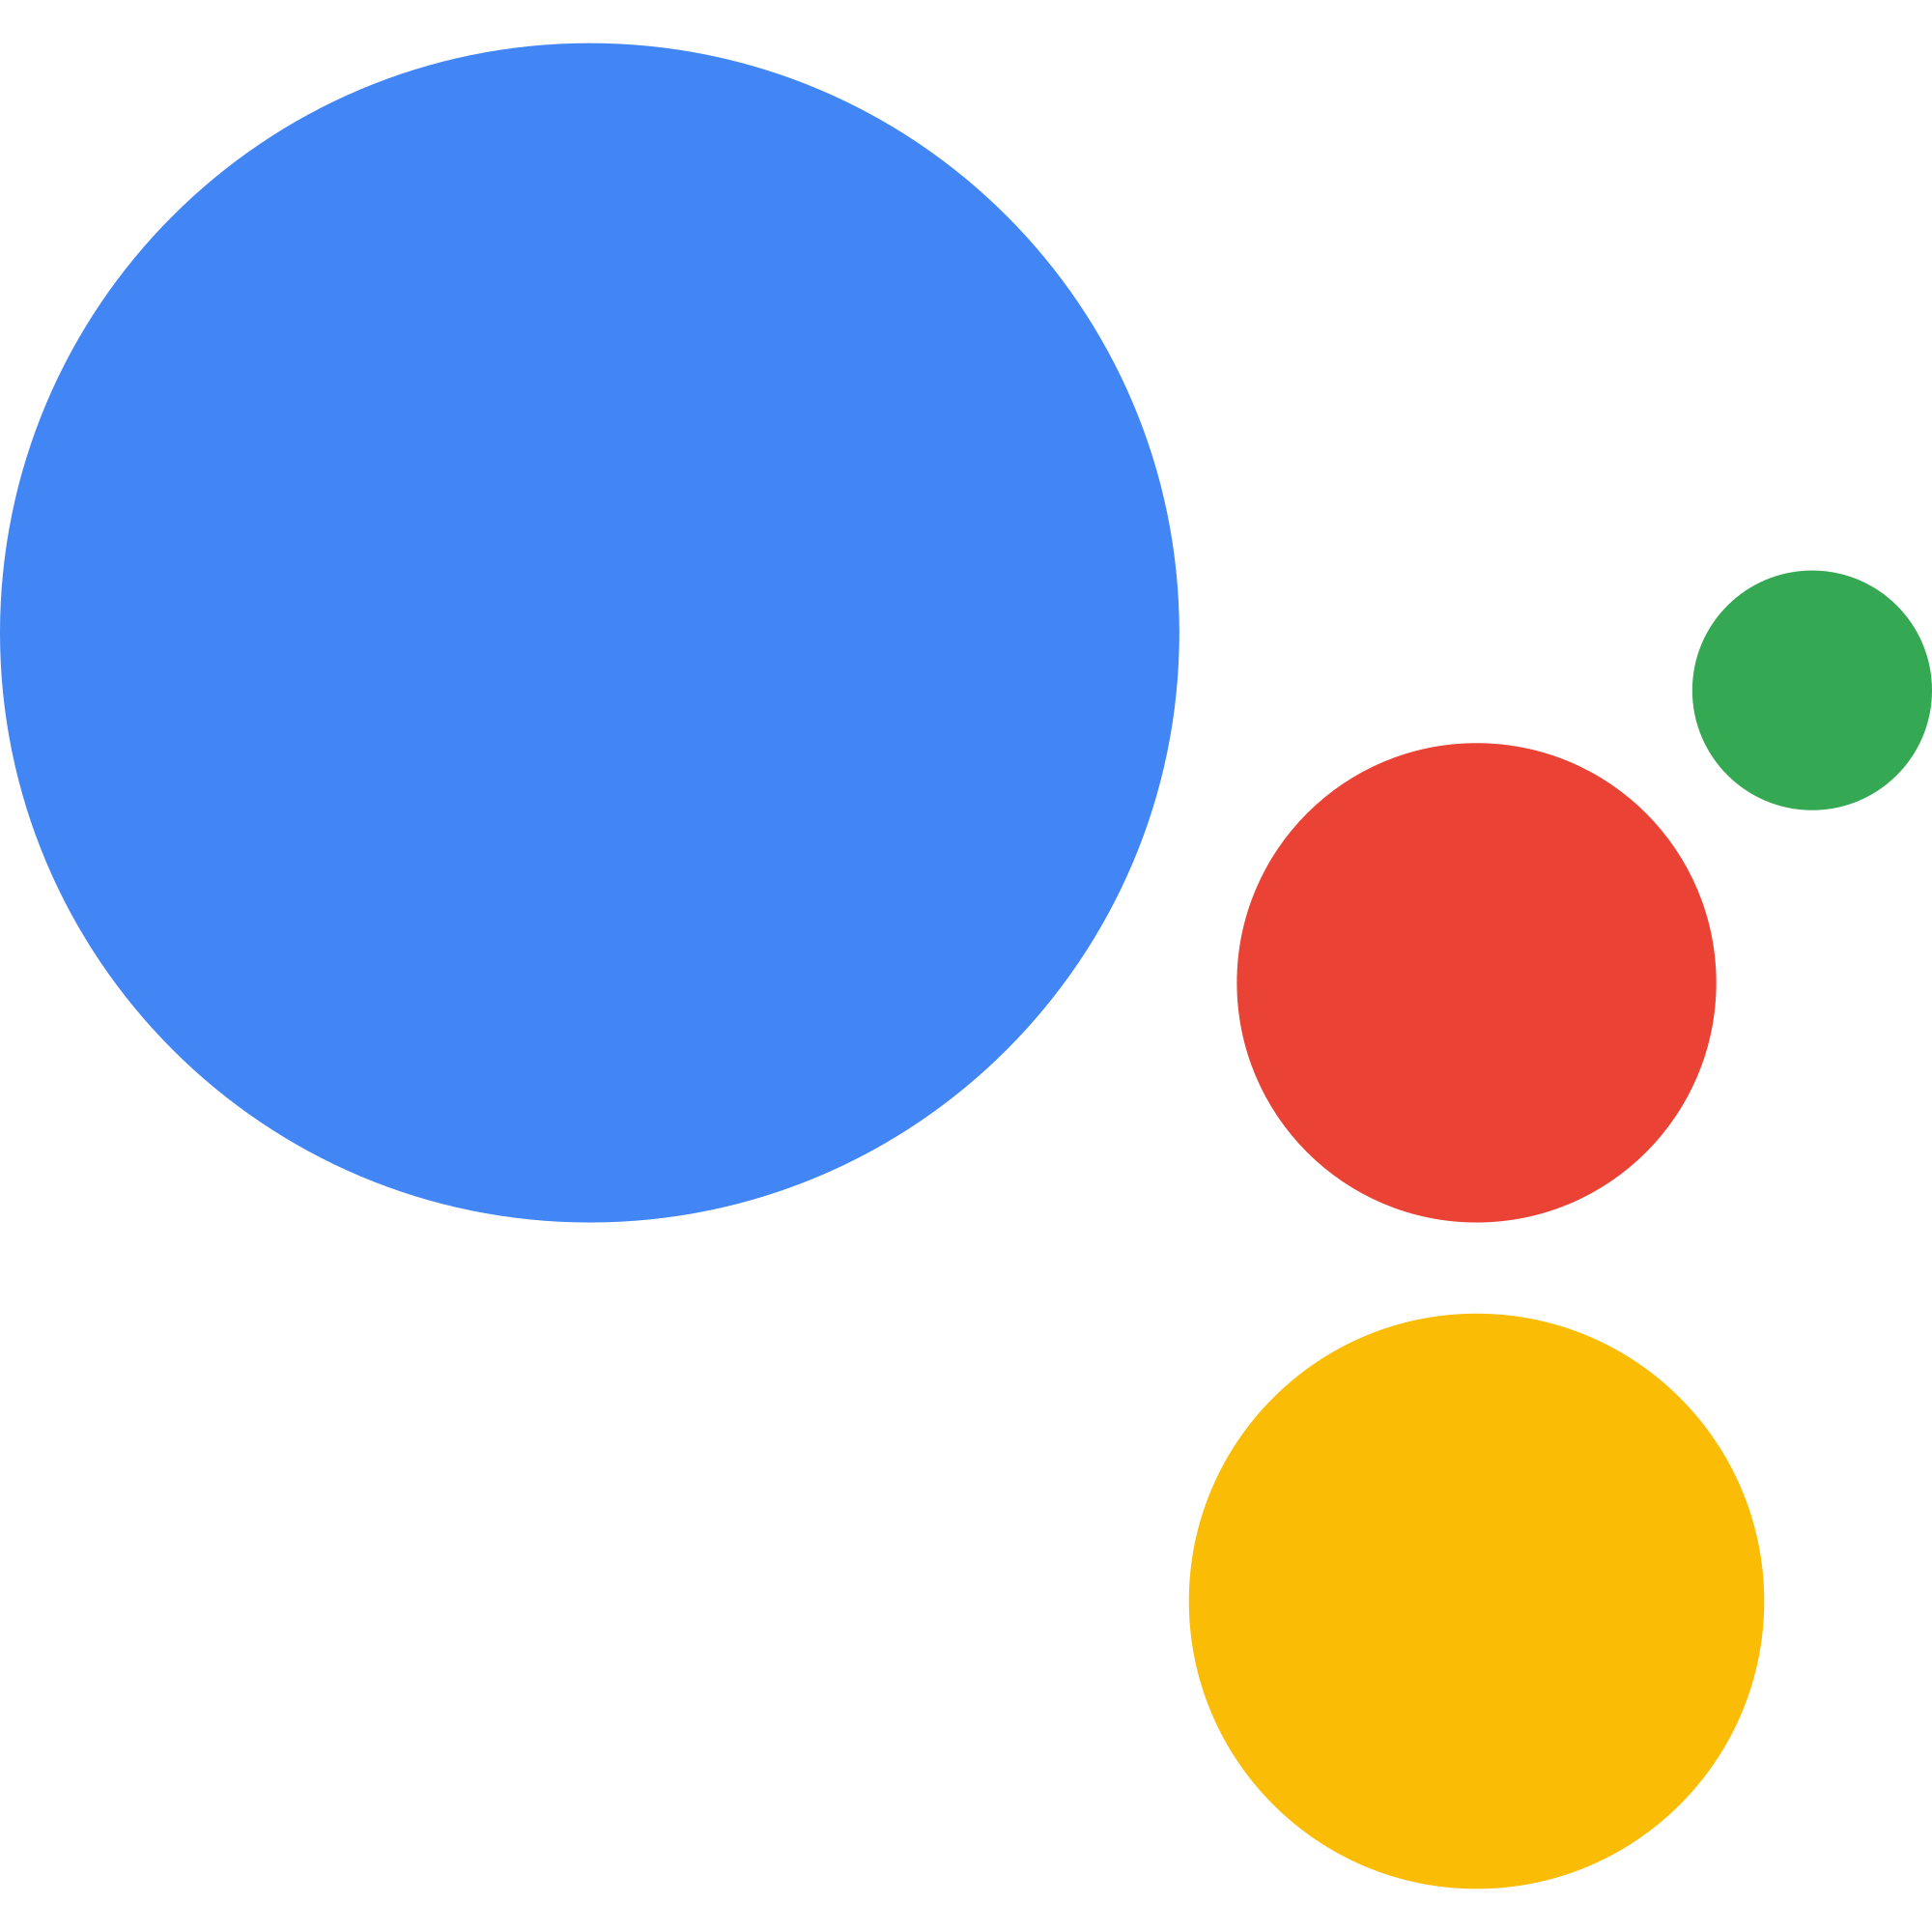
\includegraphics[width=.2\linewidth]{images/google_assitant/logo.png}
%	\caption{Logo de Google assistant} 
%\end{figure}
Lancé en 2016 sous forme d'un chatbot intégré dans l'application Google Allo,  Google Assistant s'est vu intégré directement sur les système d'exploitation Android, que ce soit sur smartphones ou tablettes, et plus récemment sur Google Home\footnote{Appareil servant à contrôler les composants d'une smart-house ainsi que l'utilisation des différents services de Google}. Google Assistant est un assistant à tout faire, Il a été développé par les ingénieurs de Google dans le but de faciliter la recherche sur internet, la planification des tâches, l'ajustement des réglages de l'appareil, etc. Son point fort est sa capacité à engager une conversation bi-directionnelle avec l'utilisateur, assurant ainsi une interaction personnalisée variant d'un utilisateur à un autre. Cette capacité lui permet par exemple de proposer certains résultats de recherche selon les précédentes interactions avec l'utilisateur ou de lui proposer une activité si ce dernier lui mentionne qu'il s'ennuie (voir figure \ref{fig:boredpic}).



\begin{figure}[h] 
	\captionsetup{justification=centering} 
	\begin{minipage}[b]{.45\textwidth}
		\centering
		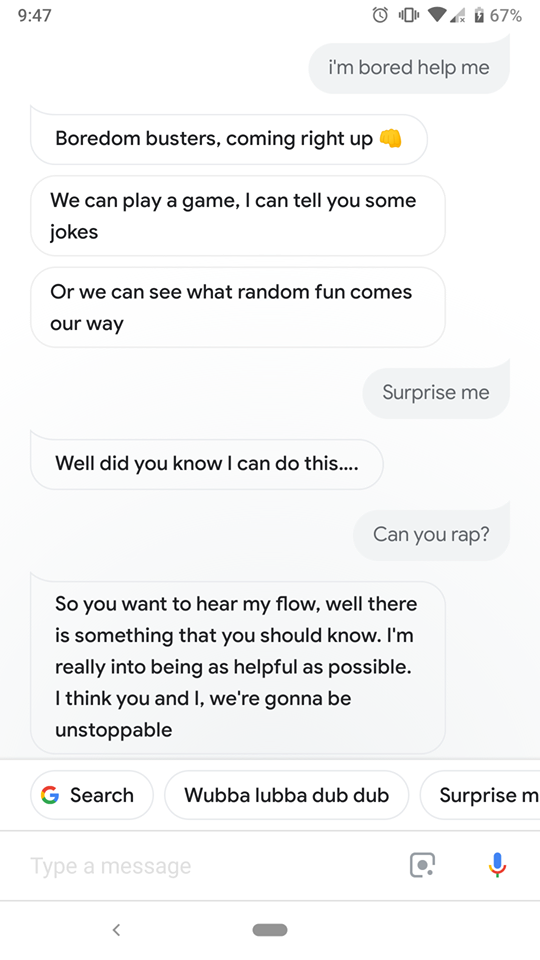
\includegraphics[width=.85\linewidth]{images/google_assitant/bored.png} 
		\caption{Conversation aléatoire avec Google Assistant}
		\label{fig:boredpic}
		
	\end{minipage}
	\hspace{0.5cm}
	\begin{minipage}[b]{.45\textwidth}
		\centering
		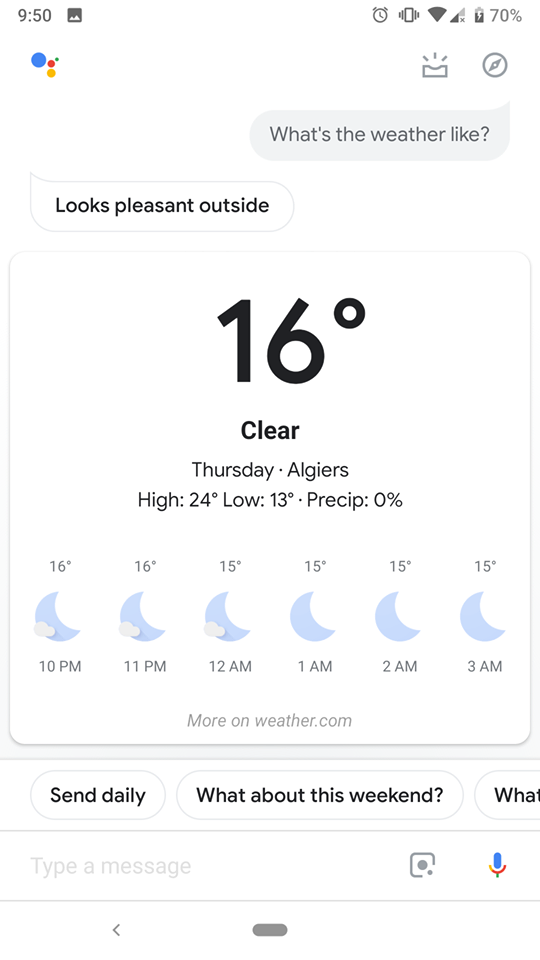
\includegraphics[width=.85\linewidth]{images/google_assitant/weather.png} 
		\caption{Requête simple formulée à Google Assitant} 
	\end{minipage}
\end{figure}


\subsubsection*{Google Duplex}\label{duplex}

\par Une des nouveautés impressionnante de Google Assistant est la fonctionnalité Google Duplex. Toujours en phase de développement, ce module est capable de passer des appels a de vraies personnes et d'avoir une conversation avec elles afin de réaliser une tâche demandée par l'utilisateur comme par exemple réserver une chambre d'hôtel, une table au restaurant, etc. 
\begin{figure}[H]
	\centering
	
\includegraphics[width=.5\linewidth]{images/google_assitant/duplex.png} 
	\caption{Google duplex réservant une place dans un salon de coiffure} 
\end{figure}


\subsection{Apple Siri}\label{siri}
%\begin{figure}[H]
%	\centering
%	
\includegraphics[width=.25\linewidth]{images/apple_siri/logo.png}
%	\caption{Logo d'Apple Siri} 
%\end{figure}
\paragraph{}
Siri est le SPA développé par Apple. Contrairement aux autres assistants virtuels qui existaient avant sa sortie, Siri proposait une nouvelle façon de communiquer avec l'utilisateur, à travers une interface de requêtes vocales, et une façon d'entretenir une conversation très humanoïde, satisfaisant ainsi le critère d'anthropomorphisme vu dans la section \ref{antropo}.
Siri est capable de proposer des recommandations, déléguer la requête à des services web ou d'autres applications (voir figures \ref{fig:whatsapp}), de répondre à des questions précises (voir figure \ref{fig:macbooksiri}). Il a l'avantage d'être uniquement disponible que sur les appareils qui composent l'écosystème d'Apple (MacBook, iPhone, iWatch, etc). Ceci assure une prise en charge et un support total de la part d'Apple. Cependant, pour utiliser l'ensemble de ses fonctionnalités, Apple restreint la liste des appareils compatibles à ceux que la compagnie fabrique uniquement. Il est ainsi quasi mono-plateforme et difficile à utiliser sur des alternatives aux produit de la firme.

\begin{figure}[H] 
	\centering
	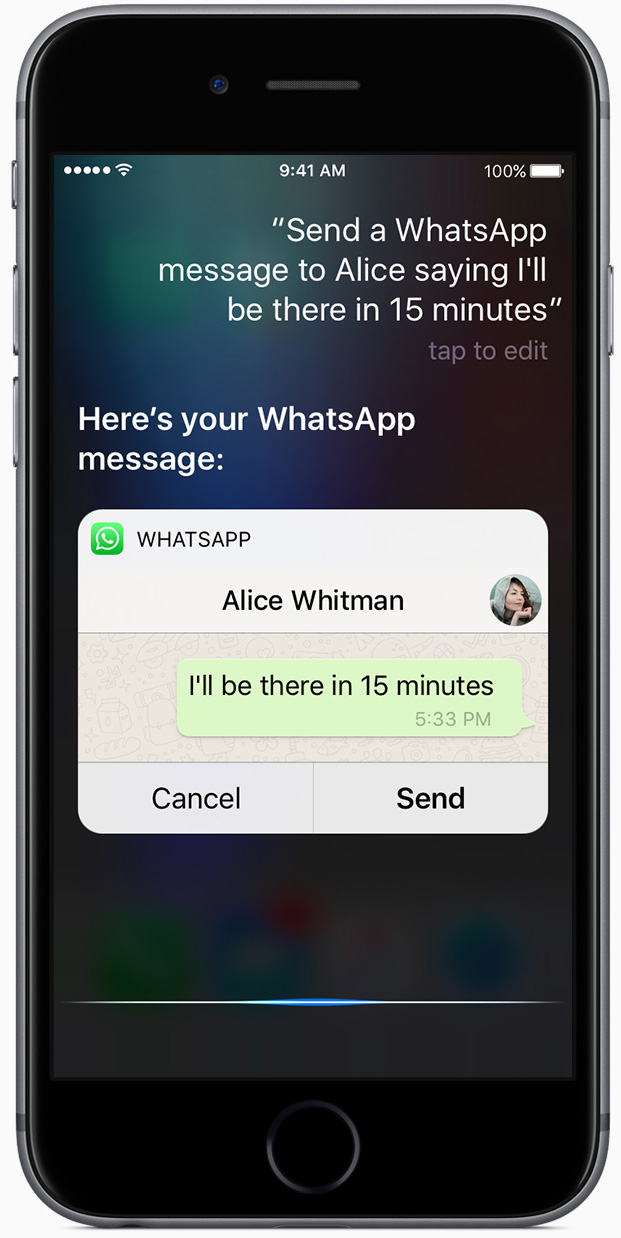
\includegraphics[width=.25\linewidth]{images/apple_siri/whatsapp.jpg} 
	\caption{Intégration aux applications \citep{siriDemo}}
	\label{fig:whatsapp}
\end{figure}


\begin{figure}[H]
	\centering
	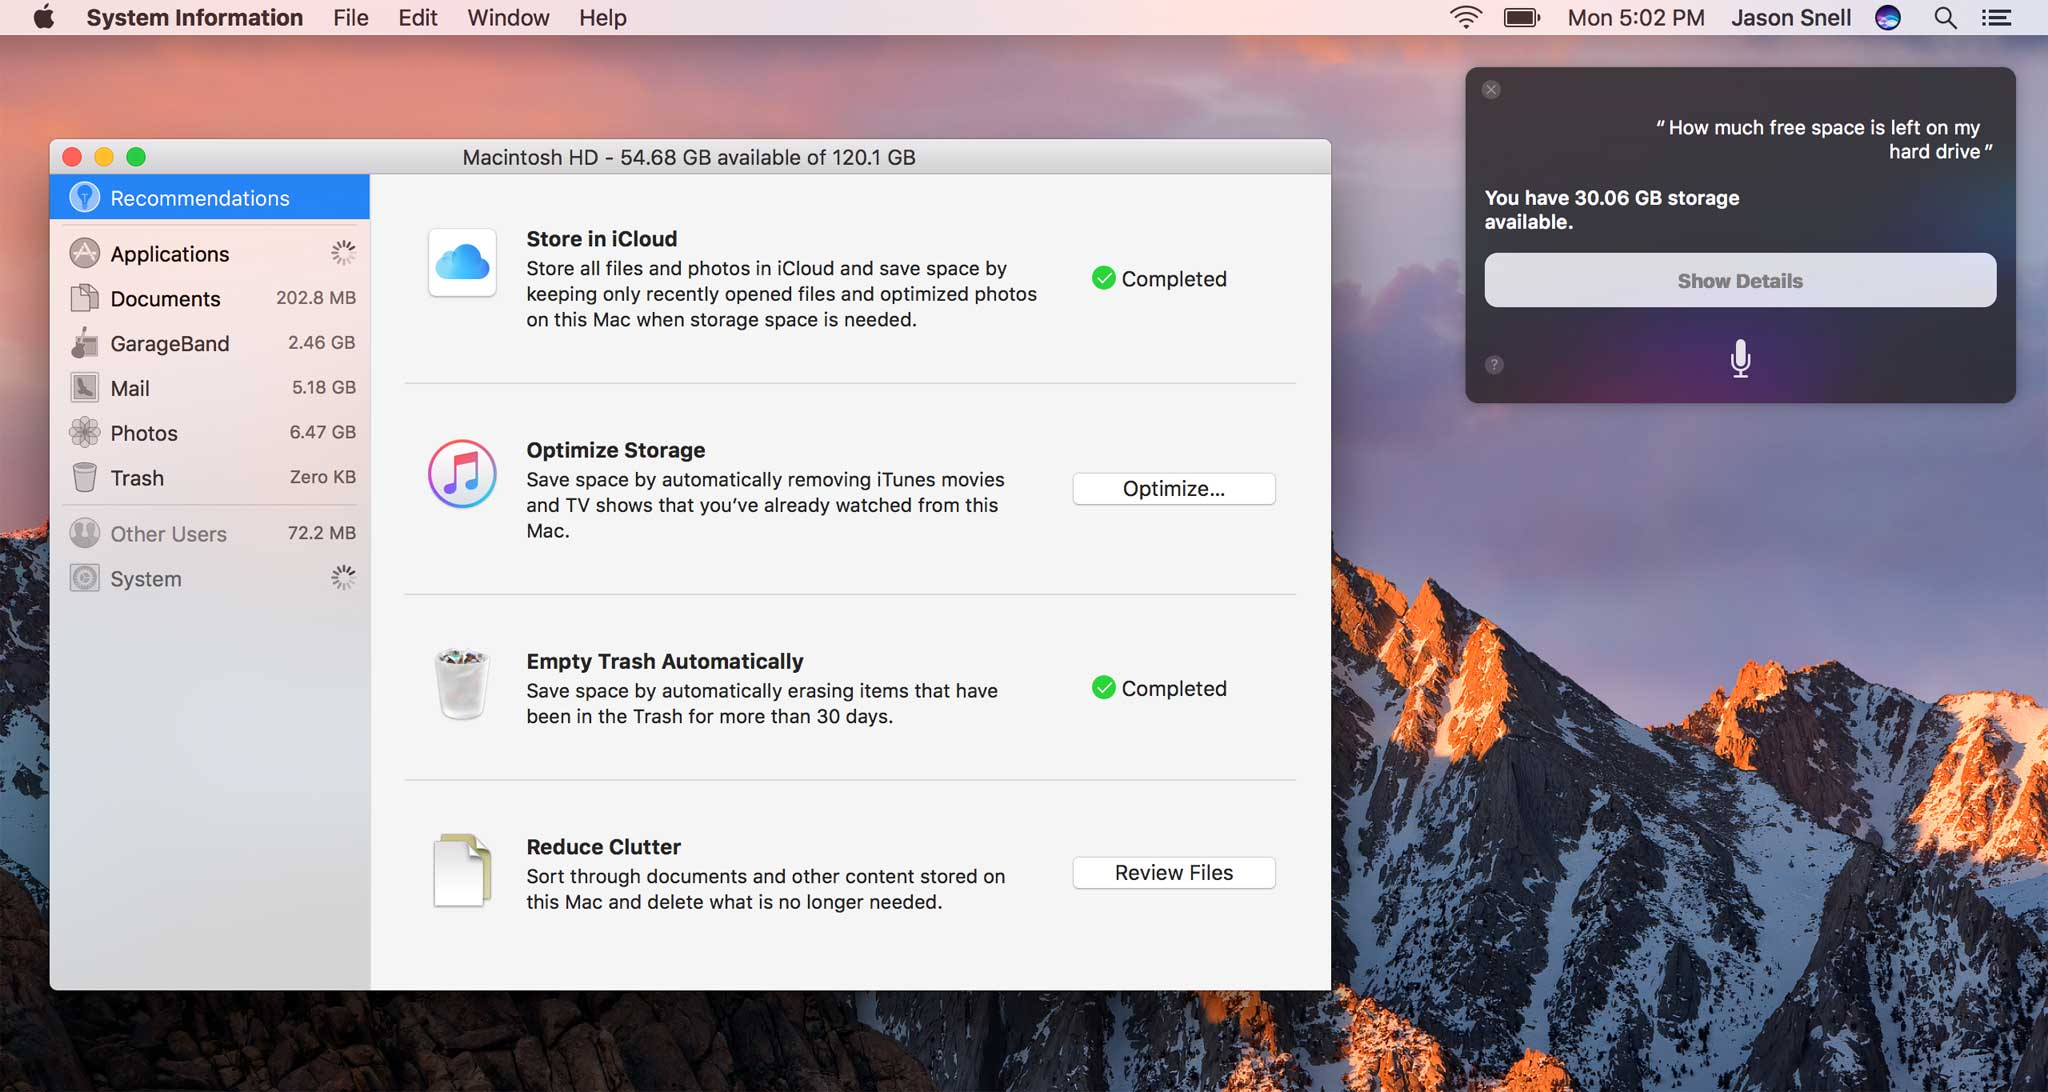
\includegraphics[width=0.75\linewidth]{images/apple_siri/macbook.png} 
	\caption{Siri sur un laptop  \citep{macossiridemo}}
	\label{fig:macbooksiri}
	
\end{figure}


\subsection{Amazon Alexa}\label{alexa}
%\begin{figure}[H]
%	\centering
%	
\includegraphics[width=.5\linewidth]{images/amazon_alexa/logo.png}
%	\caption{Logo d'Amazon Alexa} 
%\end{figure}
\paragraph{}Amazon Alexa est un assistant exclusivement intégré au dispositif Amazon Echo, un haut-parleur portatif. À l'instar de Siri, il est capable de communiquer avec l'utilisateur par le biais de la parole, pouvant ainsi exécuter diverses commandes, comme jouer de la musique, réciter des livres audios, annoncer des news en temps réel (résultats sportifs, tendances politiques, etc.). Son atout majeur est sa capacité à s'intégrer à plusieurs appareils-connectés (contrôleur de thermostat ou de lumières ambiantes dans une Smart-House) ainsi que la possibilité d'ajout des Skills (ou compétences) de la part des développeurs tiers pour enrichir la panoplie de services que peut offrir Alexa.
%\begin{figure}[H]
%	\centering
%	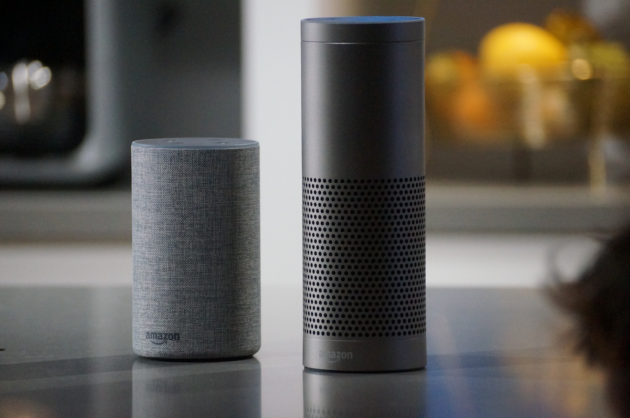
\includegraphics[width=.75\linewidth]{images/amazon_alexa/alexa.png}
%	\caption{Haut parleur Echo embarquant le SPA Alexa} 
%\end{figure}


\subsection{Microsoft Cortana}
%\begin{figure}[H]
%	\centering
%	
\includegraphics[width=.5\linewidth]{images/cortana/logo.png}
%	\caption{Logo de Microsoft Cortana} 
%\end{figure}
\paragraph{}
Cortana est la tentative de la part de Microsoft d'intégrer un assistant dans son système d'exploitation Windows 10 et WindowsPhone. Il propose divers services de base tel que planifier des tâches, exécuter des commandes via la parole, et  pour répondre à des questions, analyser des résultats de recherche sur le moteur de recherche de Microsoft, Bing.
%\begin{figure}[H]
%	\centering
%	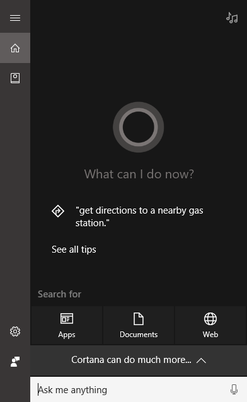
\includegraphics[width=.3\linewidth]{images/cortana/weather.png}
%	\caption{Cortana répondant à une requête utilisant Bing } 
%\end{figure}
%
%\section{Architecture générale d'un SPA}
%\paragraph{}
%Il n'existe pas vraiment d'architecture type pour un SPA. Chaque équipe de chercheurs a tenté sa propre implémentation. Après avoir étudié les différentes solutions proposées par les grandes firmes (Goole, Apple...), une représentation haut-niveau des composants d'un tel système se distingue. Nous proposons à titre d'exemple la pseudo-architecture interne de l'assistant de Google (\ref{googleass}): 
%\begin{figure}[H]
%	\centering
%	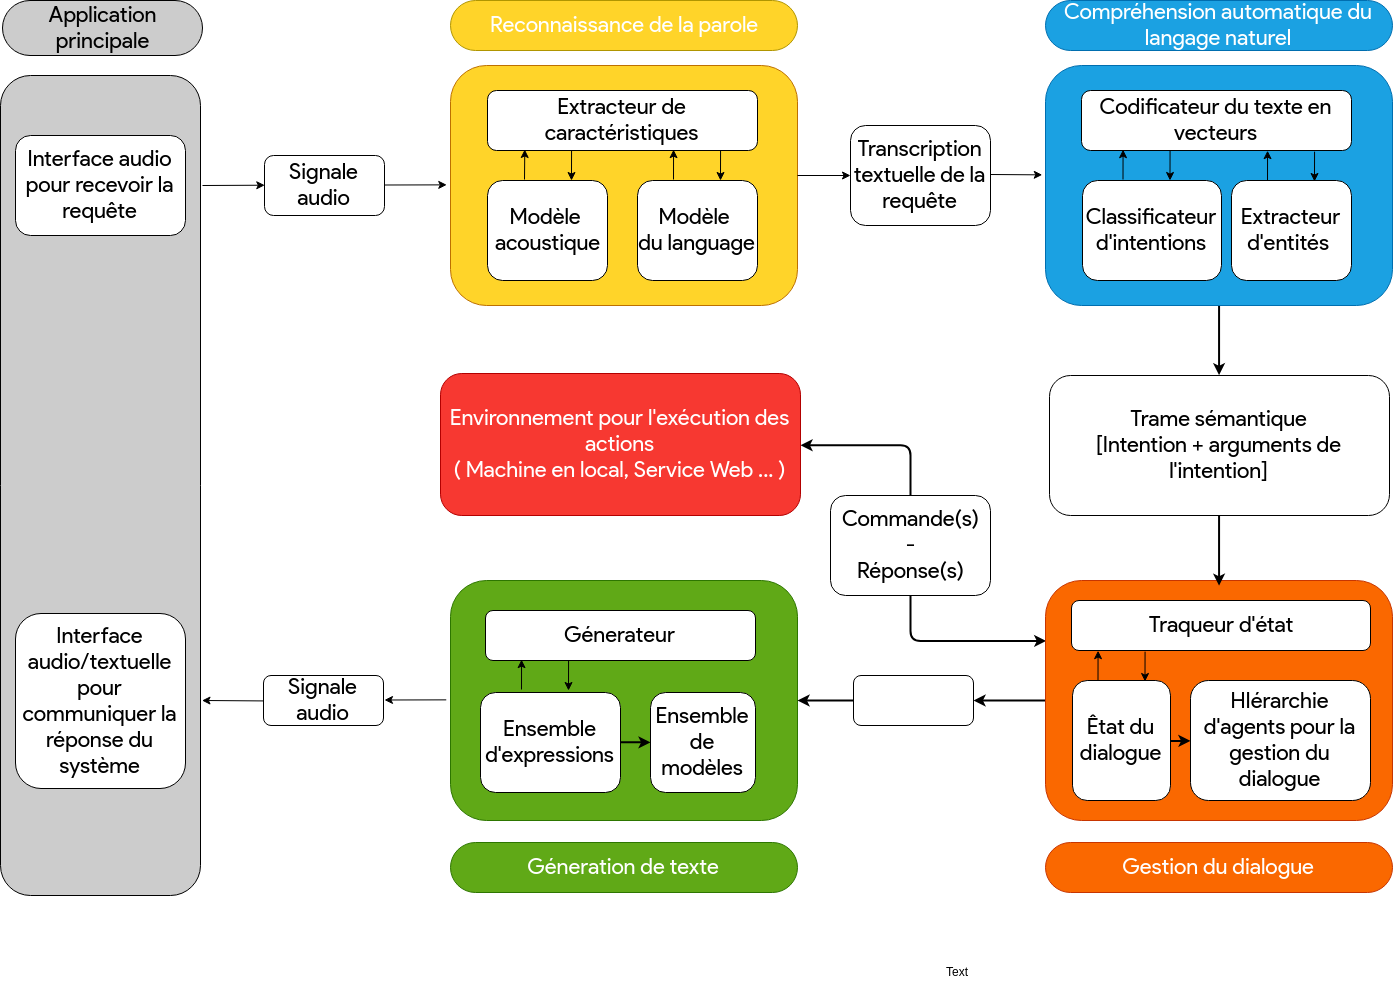
\includegraphics[width=\linewidth]{images/SPA_architecture.png}
%	\caption{Architecture haut niveau de Google Assistant \citep{GAlayout}}
%\end{figure}
%On peut ainsi dégager le schéma simplifié abstrait suivant : 
%\begin{figure}[H]
%	\centering
%	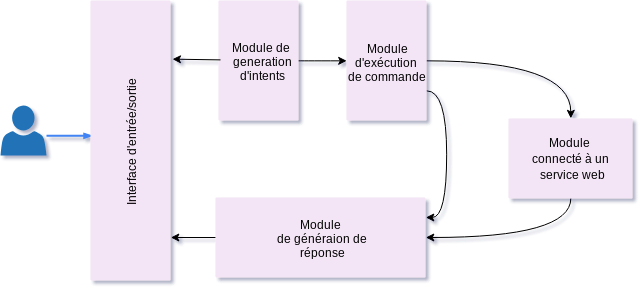
\includegraphics[width=\linewidth]{images/SPA_diagram.png}
%	\caption{Architecture abstraite d'un SPA}
%\end{figure}


%\section{Points fort des SPAs}
%\paragraph{}
%A travers les sections précédentes ,nous avons appris à découvrir les différents aspect d'un assistants virtuel intelligent, nous avons pu donc apprécié la puissance d'un tel système s'il venait à être perfectionner d'avantage.
%\par En effet, en examinant les domaines d'applications, il est facile de déduire que le recours à un SPA peut grandement faciliter certaines tâches, que ce soit pour celles qui sont les plus triviales et donc peuvent retarder d'autres tâches plus importantes, ou bien celles qui doivent faire appel à la précision ou la grande capacité de calcul des machines, assurant ainsi des résultats précis et rapidement délivrés.
%
\section{Conclusion}
\paragraph{}
À travers les sections précédentes, nous avons présenté un certain nombre d'aspects d'un assistant virtuel intelligent. Nous avons donc pu apprécier la potentielle puissance d'un tel système s'il venait à être perfectionné d'avantage.
\par En effet, en examinant les domaines d'applications, il est facile de déduire que le recours à un SPA peut grandement faciliter certaines tâches, que ce soit celles qui sont les plus triviales pouvant retarder d'autres tâches plus importantes, ou bien celles qui doivent faire appel à la précision et à la grande capacité de calcul des machines, assurant ainsi des résultats précis et rapidement délivrés.
\par
À la fin de ce chapitre nous pouvons donc mettre en valeur la place primordiale que pourraient avoir les SPAs s'ils arrivaient à maturité, c.à.d briser la barrière qui sépare les humains de la machine, parvenant ainsi à faire partie de la vie quotidienne des utilisateurs. 
\par Dans le prochain chapitre nous allons principalement aborder les aspects techniques des différents composants du SPA que nous allons réaliser.

 

\newpage
\chapter{Composants de base d'un assistant personnel}

\section{Introduction}
\paragraph{}
Dans ce chapitre, nous détaillerons un peu plus l'aspect technique d'une architecture typique d'un SPA (Speech Personal Assistant). Nous commencerons d'abord par définir des notions de base. Nous ne  traiterons que celles qui ont été les plus utilisées dans les travaux que nous avons examiné. La suite du chapitre sera organisée en sections qui décrirons chacune le fonctionnement d'une partie du SPA, en citant les travaux et références qui relatent de cette dernière. Nous terminerons sur une conclusion qui introduira le chapitre suivant.

\section{Schéma global d'un SPA}
\label{spaSchemSection}
\paragraph{}
Durant nos lectures des différents travaux sur le domaine, nous avons pu dresser un schéma assez général qui englobe les principaux modules d'un SPA : 
\begin{figure}[H]
	\centering
	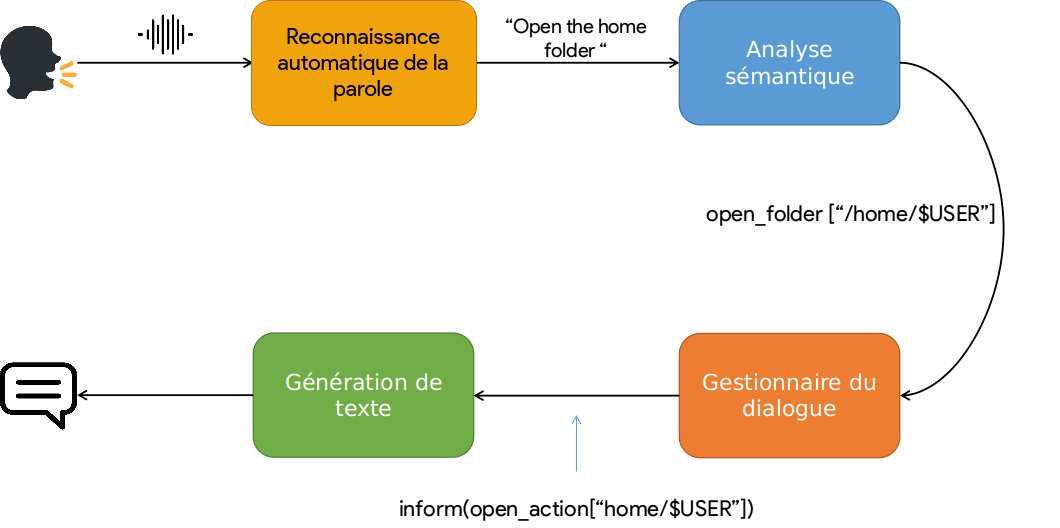
\includegraphics[width=0.8\linewidth]{images/SPA_diagram_2.png}
	\caption{Schéma abstractif d'un SPA \citep{spa_arch}}
	\label{fig:spaDiagram}
\end{figure}
\paragraph{}
Le processus peut être résumé en des étapes cruciales (qui seront détaillées dans les sections suivantes) : 
\begin{itemize}
	\label{spaLifeCycle}
	\item L'utilisateur énonce une requête en utilisant sa voix. Le signal est ensuite transformé en sa version textuelle.
	\item Étant sous un format textuel brut, la requête ne peut pas être interprétée ou comprise par la machine. Une représentation sémantique est générée qui regroupera les principales informations contenues dans la requête, à savoir l'intention de l'utilisateur et ses arguments.
	\item Au fur et à mesure que l'utilisateur énonce des requêtes, le système doit pouvoir être capable d'utiliser le contexte du dialogue pour interagir avec ce dernier afin d'atteindre le but final du dialogue (exécuter une commande système, trouver des informations internet ou sur la machine locale, etc.). Le gestionnaire du dialogue communique avec son environnement en utilisant la même représentation sémantique produite par l'analyse précédente.
	\item Puisqu'il est préférable de cacher à l'utilisateur tout comportement interne au système, il serait préférable de transformer la trame sémantique (voir la figure ~\ref{fig:semanticFrame}) en texte naturel pour l'afficher en sortie.
\end{itemize}
\paragraph{}
Il est à noter que chacun des modules seront indépendants pour ce qu'il est de leur fonctionnement interne. Ainsi, aucun n'assumera un fonctionnement arbitraire des autres modules. Seul le format des informations qui circulent entre eux devra être établi au préalable pour un fonctionnement durable et robuste au changement.
\paragraph{}
Pour ce qui est de la suite du chapitre, nous allons présenter les différents modules ainsi que les techniques et architectures qui sont considérées comme étant l'état de l'art du domaine. 

\section{Notions et aspects théoriques}
\paragraph{}
Dans cette section, nous présenterons différentes notions liées au domaine de l'apprentissage automatique, pour ensuite les citer dans les modules qui les utilisent. 
\subsection{Apprentissage automatique}
\paragraph{}
Le plus souvent, un domaine scientifique peut être défini à travers le ou les types de problèmes dont il essaye de trouver une solution. D'après \citep{mitchelllearning}, l'auteur définit ce problème sous forme d'une question :
\begin{quote}
	\say{How can we build computer systems that automatically improve with experience, and what are the fundamental laws that govern all learning processes?}\\\citep{mitchelllearning}
\end{quote}
que nous pouvons traduire par :
\begin{quote}
	\say{Comment pourrions nous développer un système informatique qui pourrait s'améliorer à travers l'expérience, et quelles seraient les lois qui régiraient le processus d'apprentissage?}
\end{quote}
\par 
D'après \citep{mitchelllearning}, l'apprentissage automatique est un paradigme qui stipule qu'un système informatique peut apprendre à effectuer un ensemble de tâches T, sachant qu'il dispose d'un ensemble de données E, tout en améliorant sa performance P.
\par
Il existe plusieurs sous-catégories d'apprentissage automatique. Elles diffèrent principalement par la manière dont le système apprend, du type de données sur lesquelles il apprend. ainsi que du but de son apprentissage (classification, régression, etc.). Nous pouvons citer les catégories suivantes :
\begin{itemize}
	\item  \textbf{Apprentissage supervisé} : Les algorithmes de cette catégorie ont besoin d'une assistance externe. Les données doivent être séparées en deux parties (ensemble d'apprentissage et de test). Un \textit{label} (ou classe) est associé à chaque instance pour permettre à l'algorithme de calculer un certain taux d'erreur qu'il essayera de minimiser au fur et à mesure qu'une nouvelle instance lui est présentée \citep{supervised_learning}. Idéalement, le système pourra apprendre une certaine fonction $\hat{f} : X \rightarrow Y$ qui liera les entrées $X$ aux sorties $Y$ en minimisant l'erreur $E_Y$ 
	
	\item \textbf{Apprentissage non supervisé} : Dans ce cas, les algorithmes ne disposent pas d'un étiquetage des données. Ils essayeront donc d'apprendre des \textit{pattern} ou motifs fréquents pour grouper les données similaires. De tels algorithmes ne se préoccupent pas de la classe, mais de la similarité entre un groupe de données et un autre \citep{unsupervised_learning}.
	
	\item \textbf{Apprentissage par renforcement} : Cette dernière catégorie regroupe des algorithmes qui apprennent par un système de \textit{trial and error} (Essais et erreur). C'est à dire qu'en interagissant avec l'environnement, l'agent apprenant (l'algorithme) apprendra à accomplir une tâche précise en exécutant des actions qui modifierons son état et celui de son environnement (voir la section \ref{reinf_learning})
\end{itemize}
\par
Dans les sections suivantes, nous nous intéresserons à quelques types d'algorithme d'apprentissage automatique. 
\subsection{Réseaux de neurones artificiels}
\paragraph{}
Un réseau de neurones artificiels est une structure d'appariement non-linéaire entre un ensemble de caractéristiques en entrée et sortie; ces réseaux sont inspirés de la façon dont les systèmes nerveux biologiques fonctionnent. Ils permettent de modéliser les relations sous-jacentes des données. Ils sont composés d'un nombre arbitrairement large de petites unités de calcul interconnectées appelées neurones, qui traitent l'information d'une manière parallèle dans le but de résoudre un problème bien spécifique \citep{neural_nets}. Ils ont notamment connu un très grand succès pendant les dernières années dans différents domaines comme la reconnaissance d'images \citep{inception}, la reconnaissance automatique de la parole \citep{speech_reco_dnn,speech_reco_Yu2015} ou encore la classification de textes \citep{seq2seq_multitask_classification,dnn_text_classification}.
\par 
Il existe une variété d'architectures de réseaux de neurones. Nous traiterons dans cette section trois d'entre elles : 
\begin{itemize}
	\item Réseaux de neurones multicouches denses
	\item Réseaux de neurones profonds
	\item Réseaux de neurones récurrents et leurs variantes
\end{itemize}
\subsubsection{Réseaux de neurones multicouches denses}

\paragraph{}
La forme la plus basique que peut avoir un réseau de neurones est celle d'un réseau multicouches comme montré dans la figure \ref{mlp}. Elle se compose de trois parties :
\begin{itemize}
	\item \textbf{Une couche d'entrée :} Elle reçoit l'information en entrée codifié en un vecteur numérique $\chi$
	
	\item  \textbf{Une ou plusieurs couches cachées :} le c\oe{}ur du réseau, c'est une succession de couches de neurones où chaque couche $C_i$ reçoit un signal sous forme d'une ou plusieurs valeurs numériques depuis une couche antérieure $C_{i-1}$ ou bien la couche d'entrée $\chi$, puis envoit en sortie un autre signal de même nature qui est une combinaison non-linéaire du signal en entrée vers une couche cachée suivante $C_{i+1}$ ou bien la couche de sortie
	\item \textbf{Une couche de sortie :}
	elle permet de calculer une valeur $\hat{y}$ qui peut être vue comme la prédiction du modèle $\Phi$ par rapport à son entrée $\chi$ : 
	\begin{equation}
	\hat{y} = f_\Phi(\chi)
	\end{equation}
\end{itemize}
Le réseau calcule une erreur $e(y,\hat{y})$ en fonction de sa valeur en sortie et de la valeur exacte puis corrigera cette erreur au fur et à mesure du parcours des données d'apprentissage \citep{mlp}
\begin{figure}[H]
	\centering
	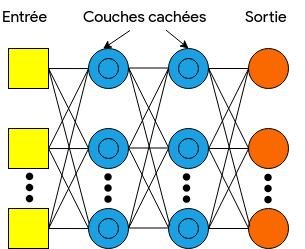
\includegraphics[width=0.5\linewidth]{images/notions/mlp.png}
	\caption{Architecture basique d'un réseau de neurones multicouches}
	\label{mlp}
\end{figure}

\subsubsection{Réseaux de neurones profonds}\label{part2DNN}
\paragraph{}
Les réseaux de neurones à une seule couche sont dits \textit{shallow}. Historiquement, ils présentaient l'avantage d'être assez rapides durant la phase d'apprentissage. Cependant les limites computationnelles d'antan se sont vite vues brisées avec le développement de processeurs plus puissants. De plus, avec l'explosion des données sur internet, toutes les conditions nécessaires étaient réunies pour la mise en place d'architectures plus complexes. Les réseaux de neurones profonds sont une adaptation des réseaux multi-couches classiques avec généralement plus de 2 couches cachées. 
\par 
Même si le principe reste le même, l'apprentissage profond est puissant car les architectures les plus complexes permettent d'extraire automatiquement les caractéristiques qui sont importantes mais non visibles; c'est le cas des réseaux de neurones convolutifs et récurrents \citep{dnn} 

\subsubsection{Réseaux de neurones récurrents}\label{seq2seqpart2}
\paragraph{}
Un aspect que les réseaux de neurones (profonds ou pas) ne peuvent capturer est la notion de séquentialité. En effet beaucoup de problèmes qui sont de nature séquentielle ne peuvent être modélisés par les architectures dites classiques, comme l'analyse d'un texte. L'introduction d'une notion de séquence permet donc de capturer des dépendances entre certains états et leurs voisins, on parle ici de contexte \citep{rnn_lstms}.
\par 
Les réseaux de neurones récurrents (Recurrent Neural Networks, RNNs) sont des réseaux de neurones \textit{feedforward} dont certaines connections en sortie sont réintroduites comme entrées dans le réseau durant une étape ultérieure du processus d'apprentissage. Ceci introduit la notion de temps dans l'architecture. Ainsi à un instant $t$, un neurone récurrent recevra en entrée la donnée $x^{(t)}$ ainsi que la valeur de l'état caché $h^{(t-1)}$ résultante de l'étape précédente du réseau, la valeur en sortie $\hat{y}^{(t)}$ est calculée en fonction de l'état caché $h^{(t)}$. Les équations suivantes montrent les calculs effectués \citep{rnn_lstms} :
\begin{equation}
h^{(t)} = \tanh(W^{hx} \times x^{(t)} + W^{hh} \times h^{(t-1)} + b_h)
\end{equation}

\begin{equation}
\hat{y}^{(t)} = softmax(W^{hy} \times h^{(t)} + b_y)
\end{equation}

où $W^{hx}$ est la matrice de poids entre la couche d'entrée et la couche cachée. $W^{hh}$ est la matrice de poids de récurrence (c.à.d, c'est la matrice qui, quand multipliée par le vecteur d'état caché $t-1$, donnera le vecteur d'état $t$). $W^{hy}$ est la matrice de poids entre la couche cachée et le couche de sortie. Les deux vecteurs $b_h$ et $b_y$ sont les vecteurs de biais et $\times$ est l'opération du produit matriciel \citep{rnn_lstms}

\begin{figure}[H]
	\centering
	%			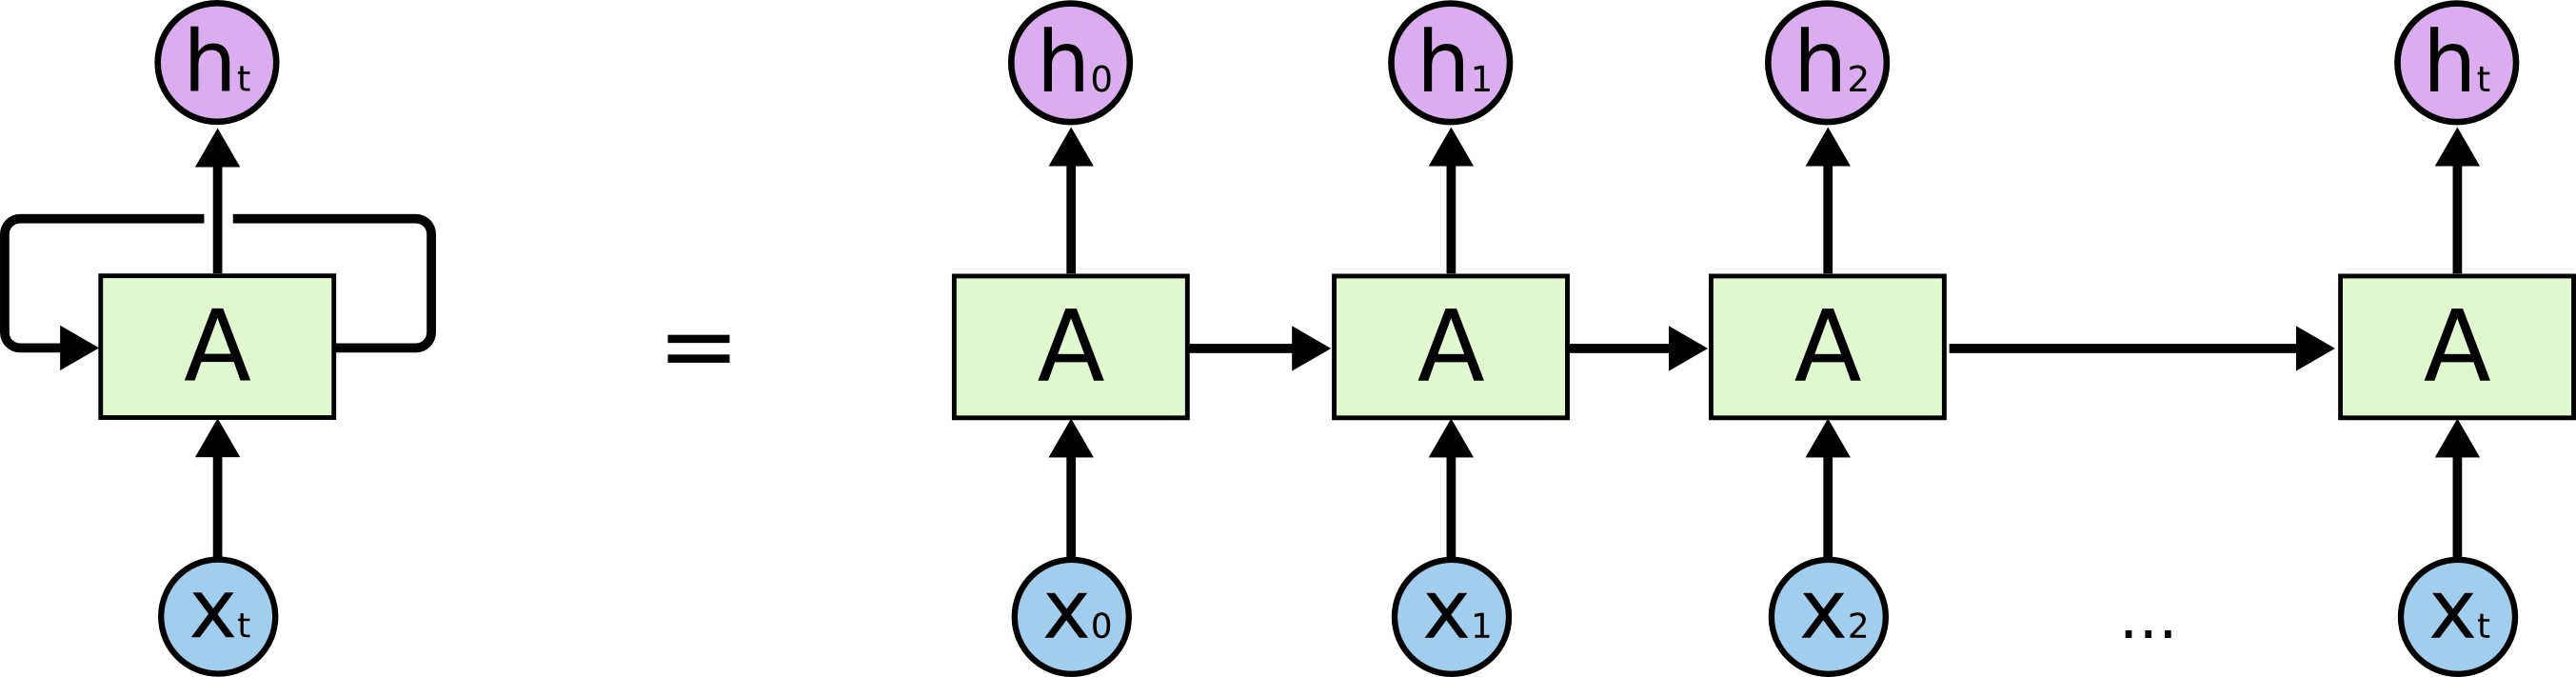
\includegraphics[width=0.5\linewidth]{images/notions/rnns.png}
	%			\caption{Un réseau de neurones récurrent durant les différentes étapes $t$ \citep{rnns_online}}
	
	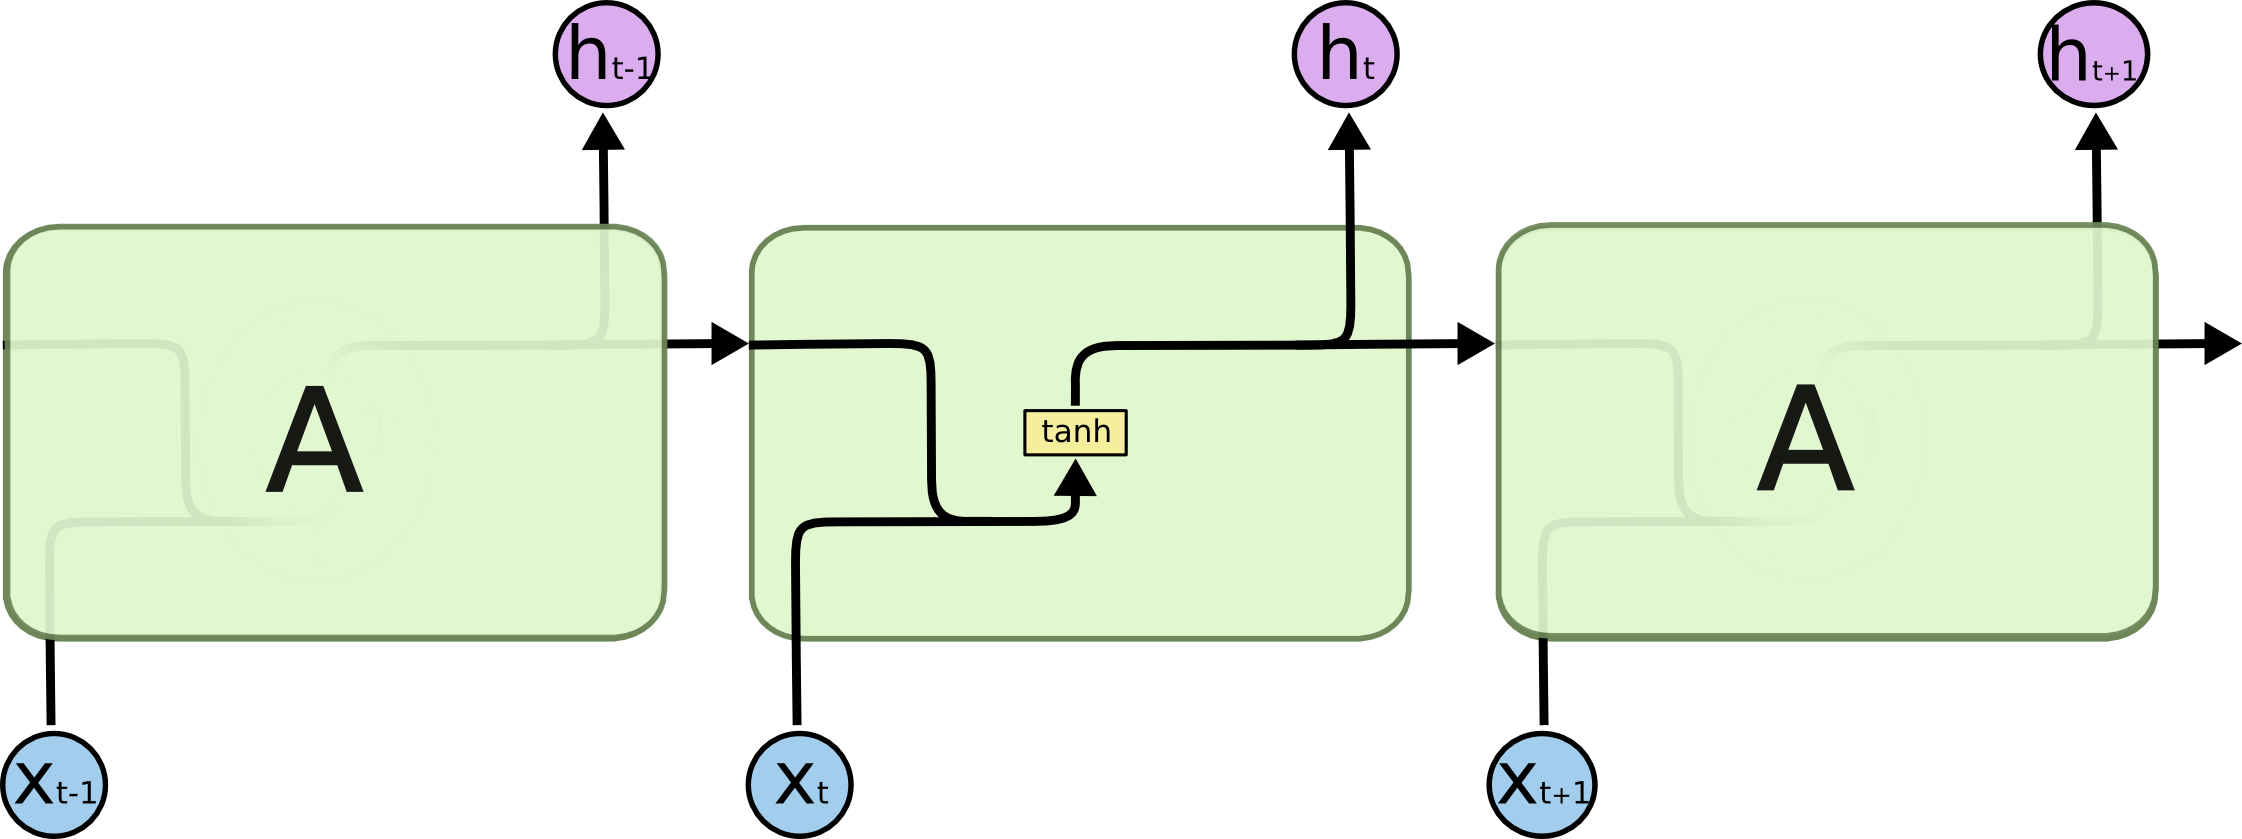
\includegraphics[width=0.5\linewidth]{images/notions/rnns_unrolled_online.png}
	\caption{Architecture interne d'un réseau de neurones récurrent à un instant $t$ \citep{rnns_online}}
\end{figure}
\par 
Un des principaux problèmes que rencontrent les RNNs est celui du \textit{"Vanishing gradient"} traduit par le \textit{"Problème de disparition du gradient"} \citep{vanishing_gradient}. Les relations à long terme entre les séquences ne sont donc pas capturées. Ainsi, pour remédier à ce problème, des architectures de réseaux de neurones dotées d'un module de mémoire ont étés introduites.

\subsubsection*{Réseaux de neurones récurrents à mémoire à court et long terme (LSTM)}
\paragraph{}
Introduite en 1997 dans \citep{lstm_original_paper}, cette architecture de réseaux de neurones récurrents est dotée d'un système de \textit{portes} qui filtrent l'information qui y passe ainsi que d'un état interne de la cellule mémoire d'un réseau LSTM. Les composants d'une cellule LSTM  sont détaillés dans la figure \ref{lstm_architecture} qui suit : 
\begin{figure}[H]
	\centering
	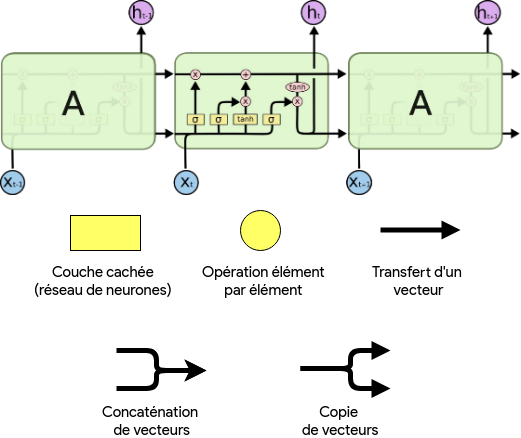
\includegraphics[width=0.5\linewidth]{images/notions/lstm_arch.png}
	\caption{Architecture interne d'une cellule mémoire dans un réseau LSTM \citep{rnns_online}}
	\label{lstm_architecture}
\end{figure}
\begin{itemize}
	\item \textbf{Porte d'entrée (Input gate): } C'est une unité de calcul qui laisse passer certaines informations en entrée en utilisant une fonction d'activation sigmoïde pour pondérer les composants du vecteur d'entrée à une étape $t$ et celles du vecteur d'état interne à l'étape $t-1$ (1: laisser passer, 0: ne pas laisser passer) et ainsi générer un vecteur candidat $\tilde{C}_t$ \citep{lstm_original_paper}.
	\begin{equation}
	\begin{gathered}
	i_t = \sigma(W_i \times [h_{t-1},x_t] + b_i) \\
	\tilde{C}_t = \tanh(W_C \times [h_{t-1},x_t] + b_C)
	\end{gathered}
	\end{equation}
	où : 
	\begin{itemize}
		\item $h_{t-1}$ et $x_t$ sont respectivement le vecteur d'état caché à l'étape $t-1$ et le vecteur de données en entrée à l'étape $t$.
		\item $\sigma$ est la fonction Sigmoïde. 
		\item $i_t$ est appelé le vecteur d'entrée de la cellule LSTM.
		\item $W_i$ est la matrice de poids entre les entrées (plus précieusement, l'état précédent et la nouvelle donnée) et le vecteur d'entrée de la cellule LSTM.
		\item $b_i$ est un vecteur de biais.
		\item $\tilde{C}_t$ est le vecteur d'état interne candidat. 
		\item $W_C$ est la matrice de poids entre le vecteur d'entrée de la cellule LSTM et le vecteur d'état interne candidat.
		\item $b_C$ est un vecteur de biais.
		\item $\tanh$ est la fonction Tangente Hyperbolique. 		
	\end{itemize}
	\item \textbf{Porte d'oubli (Forget gate): } De manière similaire, cette porte permet de spécifier au fur et à mesure de l'apprentissage les informations à oublier, qui sont donc peu importantes \citep{lstm_original_paper,rnn_lstms}.
	\newpage
	\begin{equation}
	\begin{gathered}
	f_t = \sigma(W_f \times [h_{t-1},x_t] + b_f)
	\end{gathered}
	\end{equation}
	
		où : 
	\begin{itemize}
		\item $f_t$ est appelé le vecteur d'oubli de la cellule LSTM.
		\item $W_f$ est la matrice de poids entre les entrées et le vecteur d'oubli de la cellule LSTM.
		\item $b_f$ est un vecteur de biais.		
	\end{itemize}
	\item \textbf{État interne de la cellule (Internal cell's state ): } $C_t$ est une sorte de convoyeur qui fait circuler l'information à travers la cellule. Cet état est mis à jour à travers la combinaison des deux valeurs précédemment filtrées par les portes $f_t$ et $i_t$ \citep{lstm_original_paper}.
	
	\begin{equation}
	\begin{gathered}
	C_t = f_t * C_{t-1} + i_t*\tilde{C}_t
	\end{gathered}
	\end{equation}
	où :
	\begin{itemize}
		\item $C_{t-1}$ est le vecteur d'état interne de la cellule LSTM à l'instant $t-1$.
	\end{itemize}
	\item \textbf{Porte de sortie (Output gate): } Pour renvoyer un résultat comme état interne caché du réseau, la cellule filtre son vecteur d'état et le combine avec la donnée en entrée et l'état du réseau précédent pour ne laisser passer que certaines informations \citep{rnns_online,lstm_original_paper,rnn_lstms}.
	
	\begin{equation}
	\begin{gathered}
	o_t =  \sigma(W_o \times [h_{t-1},x_t] + b_o) \\
	h_t = o_t * \tanh(C_t)
	\end{gathered}
	\end{equation}
	où :
	\begin{itemize}
		\item $o_{t}$ est un vecteur de sortie temporaire de la cellule LSTM à l'instant $t$.
		\item $W_o$ est la matrice de poids entre les entrées et le vecteur de sortie temporaire de la cellule LSTM.
		\item $b_o$ est un vecteur de biais.
			
	\end{itemize}
\end{itemize}

\subsection{Modèles de Markov cachés (Hidden Markov Models HMM)}
\paragraph{}
Informellement, un modèle de Markov caché (HMM) est un outil de représentation pour modéliser la distribution de probabilité d'une séquence d'observations. Il est dit \textit{caché} pour deux raisons. Premièrement, il est supposé qu'une observation $O$ à un instant $t$ (dénotée $O_t$)  est le résultat d'un certain processus (souvent stochastique) dont l'état $S_t$ est caché à l'observateur. Deuxièmement, l'état $S_t$ du processus caché ne dépend uniquement que de son état à l'instant $t-1$. Il est alors dit que ce processus est Markovien ou qu'il satisfait la propriété de Markov \citep{hmm_intro,markov_process}. D'une façon plus intuitive, un HMM  est utilisé pour modéliser un processus dont les observations sont régies par un autre processus caché qui ne peut être observé.
\par De façon plus formelle, un HMM est un 5-tuple $<(S,V,\Pi,A,B>$ \citep{hmm_formal} où :
\begin{itemize}
	\item $S = \lbrace s_1,...,s_N \rbrace$ est l'ensemble fini des $N$ états du processus sous-jacent.
	\item $V = \lbrace v_1,...,v_M \rbrace$ est l'ensemble des $M$ symboles qui constitue un certain vocabulaire.
	\item $\Pi = \lbrace \pi_i \rbrace$ est une distribution initiale des probabilité d'états tel que $\pi_i$ est la probabilité de se trouver à l'état $i$ à l'instant $t=0$, avec $\sum_{i=1}^{N} \pi_i = 1$ 
	\item $A=\lbrace a_{ij} \rbrace$ est une matrice $N \times N$ dont chaque entrée $a_{ij}$ est la probabilité de transition d'un état $i$ à un état $j$ avec $\sum_{j=1}^{N} a_{ij} = 1$ pour tout $i = 1,...,N$.
	\item $B=\lbrace b_i(v_k)\rbrace$ est l'ensemble des distributions de probabilités d'émission (ou d'observation), donc $b_i(v_k)$ est la probabilité de générer un symbole $v_k$ du vocabulaire étant donné un certain état $i$ avec $\sum_{k=1}^{M} b_{i}(v_k) = 1$ pour tout $i= 1,...,N$. 
	
	\begin{figure}[H]
		\centering
		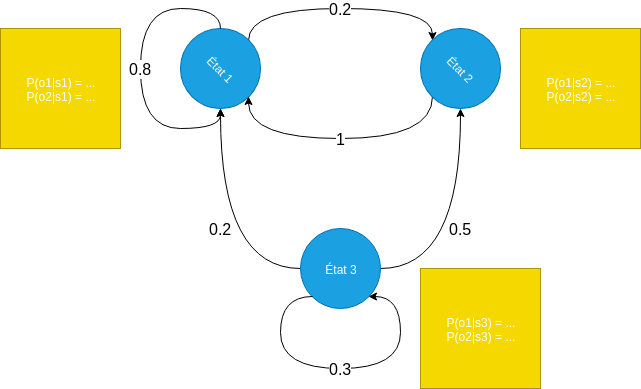
\includegraphics[width=0.65\linewidth]{images/notions/hmm.png}
		\caption{Exemple d'une distribution de probabilités de transitions ainsi qu'une distribution de probabilités d'observations pour un HMM à 3 états et 2 observations}
		\label{hmm_process}
	\end{figure}
\end{itemize}
\paragraph{}
Le but est de trouver la séquence d'états $S_{1:K}$ qui maximise la probabilité \citep{hmm_intro} : 
\begin{equation}
P(Y_{1:K} | O_{1:K}) = P(O_1)P(O_1|S_1)\prod_{t=2}^{K}P(S_t|S_{t-1})P(O_t|S_t) 
\end{equation}
Pour y parvenir d'une manière efficace, un décodeur qui implémente l'algorithme de viterbi peut être utilisé \citep{viterbi,viterbi_hmm}.

\section{Reconnaissance automatique de la parole (ASR)}
\paragraph{}
Le premier module qui compose le système est celui de la reconnaissance automatique de la parole (ASR). Le but d'un tel système (ou sous-système dans notre cas) est de convertir un signal audio correspondant à la locution d'un utilisateur en un texte qui peut être interprété par la machine \citep{asr_definition}. Différentes approches ont été développées au cours des années. Une architecture s'est ensuite dégagée où les systèmes passent par deux phases : la phase d'apprentissage et la phase de reconnaissance. La première consiste à collecter les données qui constituent le corpus d'apprentissage, un ensemble de fichiers audios avec leurs transcriptions en texte et en phonèmes. Le signal est ensuite traité pour en extraire des vecteurs de caractéristiques (ou attributs). La suite de l'apprentissage consiste à initialiser le HMM, lui passer les vecteurs précédemment extraits puis l'enregistrer pour la phase suivante qui est la reconnaissance. Dans la deuxième phase, le signal audio passe par le même procédé d'extraction des attributs, en utilisant un algorithme de décodage approprié \citep{viterbi_hmm}, puis la séquence d'observations passe par le HMM et la meilleure séquence de mots est sélectionnée \citep{speech_reco_Yu2015}.
\par Une architecture assez générale s'est dégagée. Quatre modules sont impliqués dans le processus de la reconnaissance de la parole; nous les citerons dans les sections qui suivent en énumérant les modèles utilisés dans chacun.

\begin{figure}[H]
	\centering
	\label{ASRSchema}
	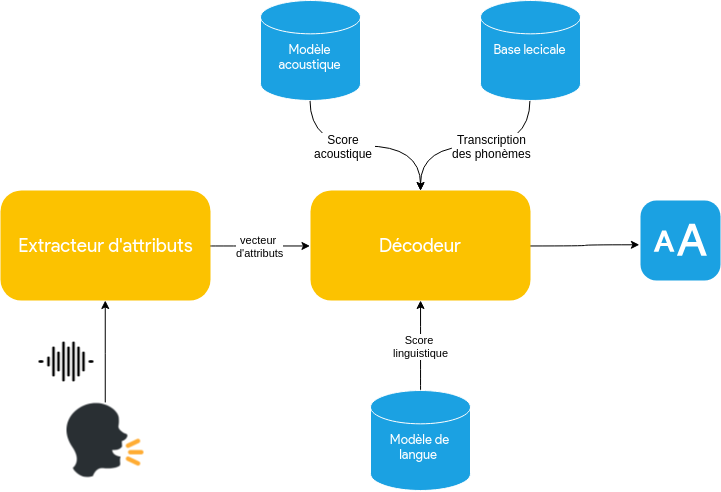
\includegraphics[width=0.70\linewidth]{images/ASR/schema.png}
	\caption{Architecture d'un système de reconnaissance de la parole \citep{speech_reco_Yu2015}}
\end{figure}

\subsection{Acquisition du signal et extraction d'attributs}
\paragraph{}
L'étape consiste à extraire une séquence de vecteurs caractéristiques à partir du signal audio, fournissant une représentation compacte de ce dernier. Le processus démarre par la segmentation du signal en \textit{trames}. Une transformation de fourrier est ensuite appliquée pour engendrer un spectre de magnitude qui sera ensuite passé à un module de transformation en spectre de Mel (Mel-Spectrum) qui est une sorte de changement d'échelle. Finalement, une transformation inverse de fourrier est appliquée pour engendrer le Mel-Cpestrum qui est le vecteur d'attributs que nous recherchions \citep{asr_extraction}. Un tel processus peut utiliser plusieurs techniques pour la mise à l'échelle: MFCC (Mel-frequency cepstrum) \citep{MFCC}, LPC (Linear Predictive coding) \citep{LSP} et RASTA (RelAtive SpecTrAl) \citep{RASTA}, chacune possédant ses avantages et ses inconvénients.
\subsection{Modélisation acoustique et modélisation du lexique}
\paragraph{}
C'est le c\oe{}ur du système de reconnaissance. Le but est de construire un modèle permettant d'identifier une séquence de phonèmes à partir d'une séquence d'observations de vecteurs d'attributs. Ceci peut être fait en utilisant un modèle HMM et en disposant d'un corpus de fichiers audio accompagnés de leurs transcriptions en phonèmes et en texte \citep{hmm_acoustic_model,hmm_formal}, ou bien un réseau de neurones profonds \citep{speech_reco_Yu2015}, ou encore une hybridation de ces derniers \citep{dnn-hmm_acoustic_model}. Le modèle acoustique procède après la reconnaissance de la séquence de phonèmes au décodage de ce dernier. Ceci est effectué en utilisant un dictionnaire linguistique qui transcrit chaque mot du vocabulaire en phonèmes qui le constituent. Ceci peut conduire à un cas d'ambiguïté où plusieurs mots peuvent avoir la même transcription phonétique (ou bien aucun mot ne correspond à cette séquence). Pour lever cette ambiguïté, un modèle de langue est nécessaire pour décider quelle est la séquence de mots la plus probable qui coïncide avec la séquence de phonèmes observée.  
\subsection{Modélisation de la langue}
\paragraph{}
Cette étape consiste à modéliser les aspects linguistiques de la langue que le système essaye de traiter. Souvent ces aspects sont spécifiques au domaine d'application afin de restreindre l'espace de recherche des mots reconnaissables par le système, puis de déterminer la séquence de mots en sortie la plus plausible. Les modèles utilisés sont basés soit sur des grammaires à contexte libre dans le cas où les séquences de mots reconnaissables sont peu variées et peuvent être modélisées par le biais de règles de la langue \citep{LM_grammar}; ou alors dans un cadre plus récent, sur des modèles probabilistes basés sur les N-grammes.
\par
\label{n-grams}
Très souvent, quand il est nécessaire de traiter un ensemble de mots, phrases ou bien toute entité atomique qui constitue une séquence, il est intéressant de pouvoir assigner une probabilité de vraisemblance à une séquence donnée (par exemple une séquence de mots). 
\par Dans un contexte textuel, un N-gramme est une suite de N mots \footnote{Dans certains cas, un N-gramme peut être aussi une suite de lettres/caractères} consécutifs qui forment une sous-chaîne $S'$ d'une chaîne de caractères $S$. Un exemple d'un ensemble de bi-grammes (2-grammes) pour la phrase "Ouvre le fichier \textit{home}" serait donc : (Ouvre,le), (le,fichier), (fichier,\textit{home}).
\par 
Ainsi, en disposant d'un corpus de textes assez large et diversifié et d'une méthode de comptage efficace, il serait possible de calculer la vraisemblance d'apparition d'un mot $w$ après une certaine séquence de mots $t$ sous forme d'une probabilité $P$ \citep{nlp_ngrams}.
\begin{equation}
P(w|t) = \frac{Comptage(t,w)}{Comptage(t)}
\end{equation}
\par
Disposant d'un volume de données textuelles assez conséquent, l'utilisation de modèles basés sur les N-grammes a prouvé son utilité \citep{nlp_ngrams,speech_reco_Yu2015,LM_n-grams} .


\section{Compréhension du langage naturel}
\paragraph{}
\label{nlu_chap2}
Après avoir obtenu la requête de l'utilisateur, le module qui prend le relais est celui de la compréhension du langage naturel (Natural Langage Understanding, NLU). Ce domaine fait partie du traitement automatique du langage naturel (Natural Langage Processing, NLP). Il se focalise principalement sur les tâches qui traitent le niveau sémantique, voire même pragmatique, de la langue tel que la classification de texte, l'analyse de sentiments ou encore le traitement automatiques des e-mails. Dans le contexte d'un SPA, le but final d'un module de compréhension du langage naturel est de construire une représentation sémantique de la requête de l'utilisateur. Étant donné une telle requête préalablement transformée en texte brut dans un langage naturel, le module essayera d'en extraire une information primordiale qui est l'intention du locuteur.

\subsection{L'intention}
\paragraph{}
L'intention est un élément clé dans notre travail. Nous allons donc la définir et expliquer pourquoi elle a été choisie comme abstraction sémantique d'une requête d'un utilisateur. \par

Une intention (ou intent en anglais) est une représentation sémantique d'un but ou d'un sous-but de l'utilisateur. Plusieurs requêtes de l'utilisateur peuvent avoir le même intent, ce qui rend l'utilisation d'une telle représentation essentielle pour que la machine puisse mieux comprendre l'utilisateur. La motivation vient du fait que la machine ne peut pas comprendre une requête formulée dans un langage non-formel. Il a fallu trouver un moyen de communication universel entre la machine et l'utilisateur de telle sorte que l'un puisse "comprendre" l'autre . L'intermédiaire entre ces deux parties est un traducteur bidirectionnel d'une requête en langage naturel vers une requête dans un langage formel et inversement. 
\par Le choix de l'intention doit être minutieusement étudié au préalable pour ne pas trop subdiviser un type d'intention, tout en gardant un certain degré de spécificité. À titre d'exemple, si deux intentions $Ouvrir\_fichier$ et $Ouvrir\_document$ existent, on retrouve ici une répétition de l'information $fichier$ qui est aussi un $document$. Dans ce cas il suffit d'éliminer un synonyme pour ne garder qu'un seul cas d'intention. \par
Un autre cas est celui du sur-découpage d'intentions déjà assez semblable, $Ouvrir\_fichier$ et $Ouvrir\_Repertoire$ peuvent être regroupés en une seule intention $Ouvrir\_Entite$. Bien-sur ces choix sont purement conceptuels et dépendent fortement du problème traité par le système. Choisir une représentation à la place d'une autre est lié à la nature de la tâche que le module doit accomplir \citep{intent_classification,intent_slots}.
\subsection{Classification d'intentions}
\paragraph{}
La classification d'intentions à partir d'un texte est une tâche réalisable avec des techniques récentes d'apprentissage automatique, plus précisément en utilisant des modèles basés sur les réseaux de neurones récurrents à "mémoire à court et long terme" (LSTM) (voir la section \ref{lstm_architecture}). Dans \citep{intent_classification} et \citep{intent_slots} deux architectures qui ont fait leurs preuves sont présentées. Dans le premier travail, les auteurs ont utilisé une architecture BiLSTM (LSTM Bidirectionnel) pour capturer les contextes droit et gauche d'un mot donné \citep{blstm}. Le dernier état caché retourné par la cellule LSTM est ensuite utilisé pour la classification. Une couche d'attention est ajoutée \citep{attention_mechanism} pour permettre au modèle de se focaliser sur certaines parties du texte en entrée. La deuxième architecture est un peu plus simple. En effet, elle utilise des cellules LSTM basiques avec une couche de classification sur le dernier état. L'avantage par rapport à la première architecture est le temps d'apprentissage assez réduit au détriment d'une erreur de classification plus accrue mais toujours dans les normes.
\begin{figure}[H]
	\centering
	\label{LSTM_intent}
	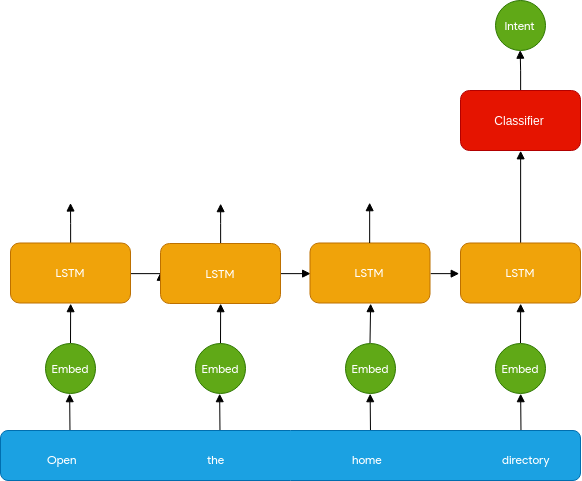
\includegraphics[width=0.65\linewidth]{images/NLU/intent_classification.png}
	\caption{Architecture de base d'un classificateur d'intentions (intents) \citep{intent_classification}}
\end{figure}
\subsection{Extraction d'entités}
\paragraph{}
Déterminer l'intention d'un utilisateur ne s'arrête pas au stade de l'identification de l'\textit{intent}. En effet, pour mieux représenter l'information récoltée depuis la requête, il faut en extraire des entités (nommées ou spécifiques du domaine) qui seront des arguments de l'intent identifié. Cette tâche consiste donc, pour une intention $I$ donné, à extraire les arguments $Args$ qui lui sont appropriés depuis le texte de la requête. Plusieurs approches sont possibles. Dans \citep{intent_slots} les auteurs ont attaqué le problème comme étant la traduction d'une séquence de mots en entrée en une séquence d'entités en sortie; le schéma suivant explicite le processus :
\begin{figure}[H]
	\centering
	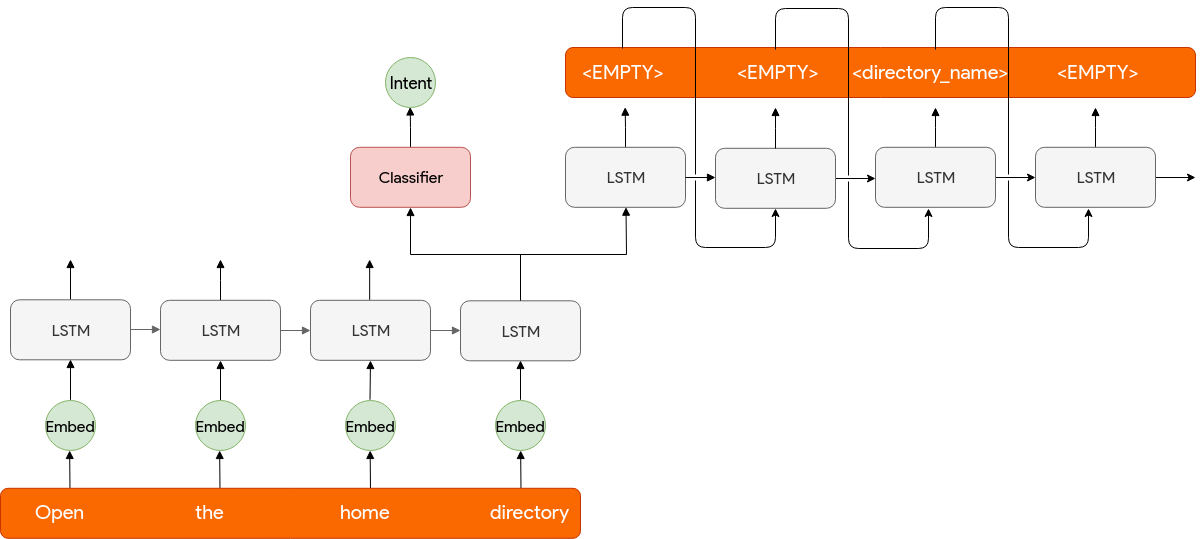
\includegraphics[width=0.85\linewidth]{images/NLU/seq2seq.png}
	\caption{Architecture de base d'un classificateur d'intentions doublé d'un extracteur d'entités \citep{intent_slots}}
	\label{fig:lstmslots}
\end{figure} 
\subsection{Analyse sémantique}
\paragraph{}
Disposant des deux modèles précédemment cités, le module NLU peut construire une représentation sémantique adéquate qui va être transmise au module suivant qui sera le gestionnaire du dialogue. L'avantage d'avoir en sortie une structure sémantique universelle est la non-dépendance par rapport à la langue de l'utilisateur. En effet, le système pourra encore fonctionner si une correspondance entre la nouvelle langue et le format choisi pour la représentation sémantique peut être trouvée. Le module donnera donc en sortie une trame sémantique (Semantic frame) qui comprendra les informations préalablement extraites, à savoir l'intention et les arguments (slots) qui lui sont propres \citep{intent_classification,intent_slots,semantic_frame}.
\begin{figure}[H]
	\centering
	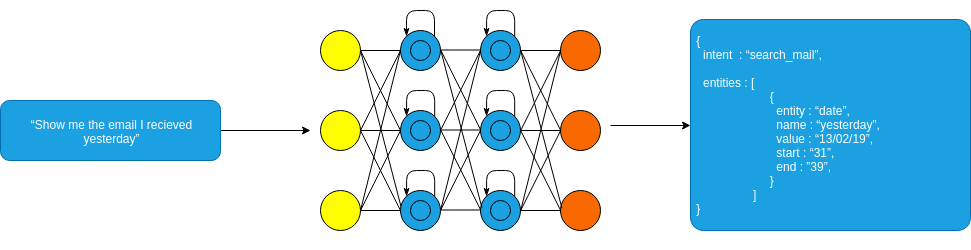
\includegraphics[width=0.80\linewidth]{images/NLU/semantic_frames.png}
	\caption{Exemple d'une trame sémantique pour une requête donnée}
	\label{fig:semanticFrame}
\end{figure} 
\section{Gestion du dialogue}
\paragraph{}
La compréhension du langage naturel permet de transformer un texte en une représentation sémantique. Afin qu'un système puisse réaliser un dialogue aussi anthropomorphe que possible, il doit décider, à partir des représentations sémantiques reçues au cours du dialogue, quelle action prendre à chaque étape de la conversation. Cette action est transmise au générateur du langage naturel (voir \ref{NLG}) pour afficher un résultat à l'utilisateur. Généralement, deux principaux modules sont présents dans les systèmes de gestion de dialogue:
\begin{itemize}
	\item Un module qui met à jour l'état du gestionnaire de dialogue: le traqueur d'état.
	\item Un module qui détermine la politique d'action du gestionnaire de dialogue.
\end{itemize}

\begin{figure}[H]
	\centering
	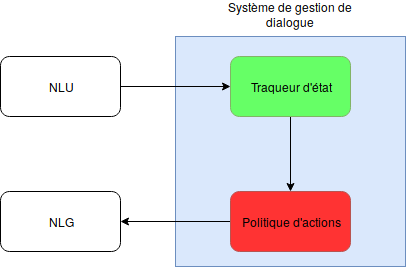
\includegraphics[width=.7\linewidth]{images/DM/DMGeneral.png} 
	\caption{Schéma général d'un gestionnaire de dialogue} 
\end{figure}
\par Ainsi, le gestionnaire de dialogue passe d'un état à un autre après chaque interaction avec l'utilisateur. Le problème à résoudre est donc de trouver la meilleure action à prendre en étant dans un état donné.
%\subsection{Processus de décision Markovien (MDP)}
\subsection{Modélisation}\label{MDP}
\paragraph{}Pour résoudre ce problème, un gestionnaire de dialogue peut être modélisé par un processus de décision Markovien (Markovian Decision Process, MDP) \citep{Bel1957}. Ce dernier est modélisé par un 4-tuple ($S,A,P,R$):
\begin{itemize}
	\item $S$: ensemble des états du système.
	\item $A$: ensemble des actions du système.
	\item $P$: distribution de probabilités de transitions entre états sachant l'action prise. $P(s'/s,a)$ est la probabilité de passer à l'état $s'$ sachant qu'on était à l'état $s$ après avoir réalisé l'action $a$.
	\item $R$: est la récompense reçue immédiatement après avoir changé l'état avec une action donnée. $R(s'/s,a)$ est la récompense reçue après être passé à l'état $s'$ sachant que le système était à l'état $s$ après avoir réalisé l'action $a$.
\end{itemize}
Un MDP, à tout instant $t$, est dans un état $s$. Dans notre cas c'est l'état du gestionnaire de dialogue. Il peut prendre une action $a$ afin de passer à un nouvel état $s'$. De ce fait, il reçoit une récompense qui ,dans notre cas, est une mesure sur les performances du système de dialogue. Le but est de maximiser les récompenses reçues.

\begin{figure}[H]
	\centering
	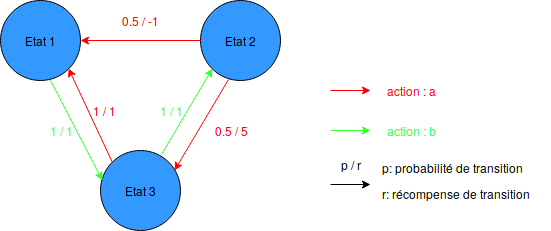
\includegraphics[width=.95\linewidth]{images/DM/MDP.png} 
	\caption{Schéma représentant les transitions entre états dans un MDP} 
\end{figure}


\subsection{État du gestionnaire de dialogue}\label{trame}
\paragraph{}
L'état d'un système de dialogue est une représentation sémantique qui contient des informations sur le but final de l'utilisateur ainsi que l'historique de la conversation. La représentation souvent utilisée dans les systèmes de dialogue est celle de la trame sémantique \citep{Chen2017}. Cette structure contient des emplacements à remplir dans un domaine donné. La figure \ref{SFrame} illustre un exemple de trame sémantique.\newline
\begin{figure}[H]
	\centering
	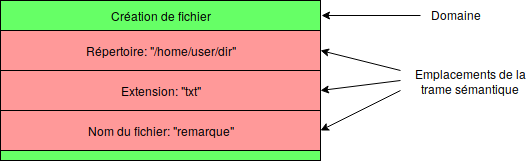
\includegraphics[width=.7\linewidth]{images/DM/SFrame.png} 
	\caption{Schéma représentant une trame sémantique avec comme domaine: création de fichier} 
	\label{SFrame}
\end{figure}


À l'arrivée d'une nouvelle information, un module dédié met à jour l'état du gestionnaire de dialogue. Comme l'action du système de dialogue est décidée à partir de son état, cette tâche est donc essentielle au bon fonctionnement du système. Plusieurs méthodes ont été proposées pour gérer le suivi de l'état du gestionnaire de dialogue \citep{Williams2007}.
\subsubsection{Suivi de l'état du gestionnaire de dialogue avec une base de règles}\label{suivi}
\paragraph{}
La méthode traditionnelle utilisée consiste à écrire manuellement les règles à suivre lors de l'arrivé d'une nouvelle information pour mettre à jour l'état \citep{Goddeau1996}. Cependant, les bases de règles sont très susceptibles à faire des erreurs \citep{Chen2017} car elles sont peu robustes face aux incertitudes.


\begin{figure}[H]
	\centering
	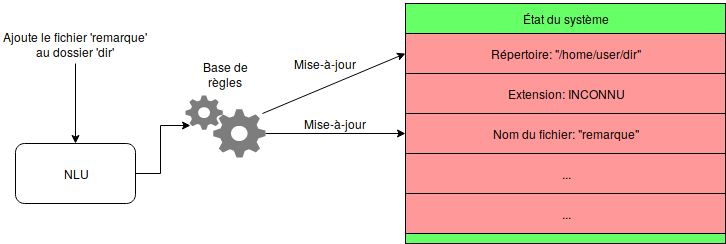
\includegraphics[width=.7\linewidth]{images/DM/RuleBasedUpdate.png} 
	\caption{Schéma représentant la mise-à-jour de l'état du gestionnaire de dialogue par un système basé règles} 
\end{figure}

\subsubsection{Suivi de l'état du gestionnaire de dialogue avec des méthodes statistiques}

Le suivi dans ce cas se fait en gardant une distribution de probabilités sur l'état du système, ce qui nécessite une nouvelle modélisation non déterministe du problème. Les processus de décision markoviens partiellement observables (Partially Observable Markov Decision Process POMDP) \citep{Young2010} sont une variante des MDP capable de répondre à ce besoin que nous introduirons par la suite. Dans ce cas, le système garde une distribution de probabilités sur les valeurs possibles des différents emplacements de la trame sémantique.

\begin{figure}[H]
	\centering
	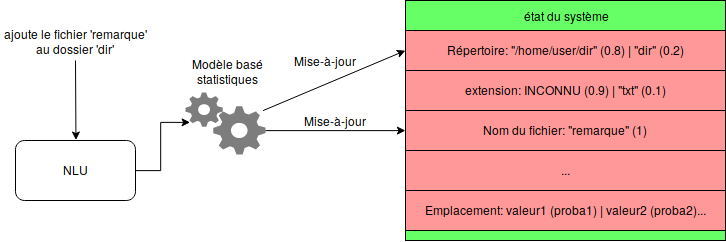
\includegraphics[width=.7\linewidth]{images/DM/StatBasedUpdate.png} 
	\caption{Schéma représentant la mise-à-jour de l'état du gestionnaire de dialogue par un système basé statistiques} 
\end{figure}

\paragraph{Processus de décision markovien partiellement observable (POMDP)}
Comme dans les processus de décision markoviens, un POMDP \citep{Astrom1965} passe d'un état à un autre en prenant une des actions possibles. Cependant, un POMDP ne connait pas l'état exact dans lequel le système se trouve à un instant $t$. Il reçoit par contre une observation qui est, dans notre cas, l'action de l'utilisateur, à partir de laquelle il peut estimer une distribution de probabilités sur l'état actuel. Pour résumer, un POMDP est un 6-tuple ($S,A,P,R,M,O$) où:
\begin{itemize}
	\item Les 4 premiers composants sont les mêmes que ceux d'un MDP (voir \ref{MDP}).
	\item $M$: l'ensemble des observations.
	\item $O$: la distribution de probabilités sur les observations $o$ en connaissant l'état $s$ et l'action $a$ prise pour y arriver. $O(o|s,a)$ est la probabilité d'observer $o$ sachant que le système se trouve à l'état $s$ et qu'il a pris l'action $a$ pour y arriver.
\end{itemize}

\begin{figure}[H]
	\centering
	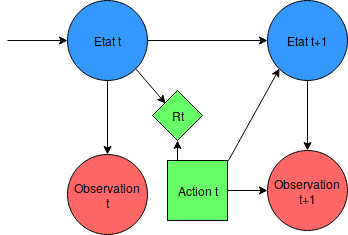
\includegraphics[width=.5\linewidth]{images/DM/POMDP.png} 
	\caption{Diagramme d'influence dans un POMDP} 
\end{figure}

\subsubsection{Suivi de l'état du gestionnaire de dialogue avec réseaux de neurones profonds}
\paragraph{}
Récemment, des approches utilisant les réseaux de neurones profonds (voir \ref{part2DNN}) ont fait leur apparition. En effet, l'utilisation des architectures profondes permet de capter des relations complexes entre les caractéristiques d'un dialogue et, ainsi, mieux estimer l'état du système. Le réseau de neurones estime les probabilités de toutes les valeurs possibles d'un emplacement de la trame sémantique \citep{Henderson2013}. En conséquence, il peut être utilisé comme modèle de suivi d'état pour un processus partiellement observable.

\subsection{Politique de gestion de dialogue}
\paragraph{}
La première partie est dédiée au module qui suit l'état du système de dialogue. Dans cette partie, nous allons présenter des approches proposées afin d'arriver au but du MDP, c'est à dire quelles actions prendre pour maximiser la somme des récompenses obtenues.
\subsubsection{Gestion de dialogue avec une base de règles}
\paragraph{}
Les premières approches utilisaient des systèmes de règles destinés à un domaine bien spécifique. Elles étaient déployées dans plusieurs domaines d'application pour leur simplicité. Cependant, le travail manuel nécessaire reste difficile à faire et, généralement, n'aboutit pas à des résultats flexibles qui peuvent suivre le flux du dialogue convenablement \citep{Lee2010}.
\subsubsection{Gestion de dialogue par apprentissage}
\paragraph{}
La résolution d'un MDP revient à trouver une estimation de la fonction de récompense afin de pouvoir choisir la meilleure action. La majorité des approches récentes utilise l'apprentissage par renforcement dans le but d'estimer la récompense obtenue par une action et un état donnés. Cette préférence par rapport aux approches supervisées revient à la difficulté de produire des corpus de dialogues \citep{Henderson2008}, encore moins des corpus annotés avec les récompenses à chaque transition. Néanmoins, il existe des approches de bout en bout qui exploitent des architectures avec réseaux de neurones profonds et traitent le problème comme Seq2Seq\footnote{Les modèles Seq2Seq sont des architectures de réseaux de neurones profonds qui prennent en entrée une séquence et produisent en sortie une autre séquence en utilisant les réseaux de neurones récurents (RNN).} afin de produire directement une sortie à partir des informations reçues de l'utilisateur \citep{Wen2017,Serban2016}.


\begin{figure}[H]
	\centering
	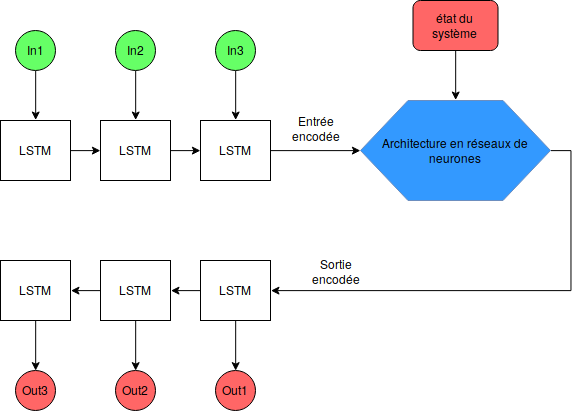
\includegraphics[width=.7\linewidth]{images/DM/DMSeq2Seq.png} 
	\caption{Schéma de gestion de dialogue de bout en bout avec architecture Seq2Seq} 
\end{figure}
\subsubsection{Apprentissage par renforcement} \label{reinf_learning}
\paragraph{}
L'apprentissage par renforcement est une approche qui a pour but d'estimer une politique d'actions à prendre dans un environnement donné. Cette politique doit maximiser une mesure d'évaluation qui est sous forme de récompenses obtenues après chaque action \citep{Weisz2018}. L'environnement est souvent modélisé comme un MDP, ou éventuellement POMDP. L'agent d'apprentissage passe donc d'un état à un autre en prenant des actions dans cet environnement. L'apprentissage se fait dans ce cas en apprenant par l'expérience de l'agent, à savoir les récompenses obtenues par les actions prises dans des états donnés. Il peut ainsi estimer la fonction de récompense pour pouvoir faire le choix d'actions optimales. 

\begin{figure}[H]
	\centering
	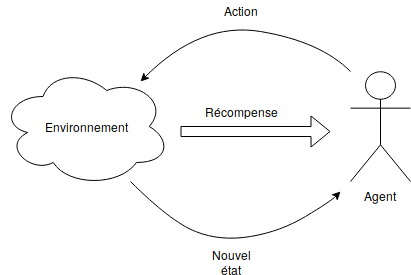
\includegraphics[width=.5\linewidth]{images/DM/RLSchema.png} 
	\caption{Schéma d'interaction agent-environnement dans l'apprentissage par renforcement} 
\end{figure}
Il existe plusieurs méthodes que l'agent peut utiliser pour estimer la fonction de récompense \citep{Dimitri2012}, notamment Deep Q Learning (DQN) \citep{Mnih2015} qui utilise les réseaux de neurones profonds pour trouver une approximation à cette fonction. Dans cette approche, à chaque fois que l'agent prend une action, il compare la récompense reçue avec celle estimée par le réseau de neurones, et applique ensuite l'algorithme de rétro-propagation pour corriger les erreurs du réseau. 

\paragraph{}
Le système de dialogue est modélisé par un MDP. Seulement, ce dernier inclut l'utilisateur comme partie de l'environnement. Par conséquent, pour appliquer l'apprentissage par renforcement, il est nécessaire qu'un utilisateur communique avec le système pour qu'il apprenne. D'où la nécessité d'utiliser un \textbf{simulateur d'utilisateur} qui est un programme capable de se comporter comme un humain interagissant avec un système de dialogue. Le simulateur doit pouvoir estimer la satisfaction de l'utilisateur après une interaction. En d'autres termes, il doit comporter une fonction de récompense. Il existe plusieurs méthodes pour créer un simulateur d'utilisateur:
\begin{itemize}
	\item Les simulateurs d'utilisateur basés règles: dans ce cas une liste de règles est écrite manuellement et le simulateur doit les suivre pour communiquer avec le système \citep{Schatzmann2007}.
	\item Les simulateurs d'utilisateur basés n-grammes: ils traitent un dialogue comme une séquence d'actions en prenant les n-1 actions précédentes pour estimer l'action la plus probable que peut prendre le simulateur à partir des statistiques tirées d'un corpus de dialogues \citep{Georgila2005}.
	\item Les simulateurs d'utilisateur basés HMM: les états du modèle sont les états du système et les observations sont ses actions. Ainsi un HMM peut estimer l'état le plus probable du système pour prendre une action. Il existe d'autres variantes, IHMM et IOHMM, qui incluent les probabilités conditionnelles des actions de l'utilisateur sachant l'état du système ou l'action du système directement dans le modèle HMM \citep{Cuayhuitl2005}.
	\item Les simulateurs d'utilisateur avec apprentissage par renforcement: Comme le gestionnaire de dialogue, le simulateur apprend par renforcement au même temps. Dans ce cas la fonction de récompense pour les deux agents peut être apprise à partir des dialogues humain-humain \citep{Chandramohan2011}.
\end{itemize}







\section{Génération du langage naturel (Natural Language Generation, NLG)}\label{NLG}
\paragraph{}
Le domaine de la génération automatique du langage naturel est l'un des domaines dont les limites sont difficiles à définir \citep{evans2002}. Il est vrai que la sortie d'un tel système est clairement du texte. Cependant, l'ambiguïté se trouve dans ses entrées, c'est-à-dire, sur quoi se basera le système pour générer le texte. D'après \citep{Reiter:1997}, la génération du langage naturel est décrite comme étant le sous domaine de l'intelligence artificielle qui traite la construction des systèmes de génération de texte à partir d'une représentation non-linguistique de l'information. Celle-ci peut être une représentation sémantique, des données numériques, une base de connaissances ou même des données visuelles (images ou vidéos). Ceci dit, d'autres travaux, comme \citep{Labbé2012}, utilisent les mêmes techniques pour des entrées linguistiques. Enfin, la génération du langage naturel peut être très proche de la gestion de dialogue \citep{Dethlefs2014}. En effet, le texte généré doit prendre en compte l'historique de la conversation et le contexte de l'utilisateur.\newline
Il existe six tâches trouvées fréquemment dans les systèmes de génération de texte \citep{Reiter:1997}; nous les présentons dans cette section.

\subsection{Détermination du contenu}
\paragraph{}
Cette partie consiste à sélectionner les informations de l'entrée dont le système veut transmettre leur contenu sous forme de texte naturel à l'utilisateur. En effet, les données en entrée peuvent contenir plus d'informations que ce que l'on désire communiquer \citep{Yu:2007}. De plus, le choix de l'information peut aussi dépendre de l'utilisateur et de ses connaissances \citep{Dethlefs2014}. Ceci requiert de mettre au point un système qui détecte les informations pertinentes à l'utilisateur.
\subsection{Structuration de texte}
\paragraph{}
Après la détermination du contenu, le système doit ordonner les informations à transmettre. Ceci dépend grandement du domaine d'application qui peut exiger des contraintes d'ordre temporel ou de préférence par importance des idées. Les informations à transmettre en elles-mêmes sont souvent reliées par sens, ce qui implique une certaine structuration de texte à respecter.\newpage
\subsection{Agrégation de phrases}
\paragraph{}
Certaines informations peuvent être transmises dans une même phrase. Cette partie introduit des notions de la linguistique afin que le texte généré soit plus lisible et éviter les répétitions. Un exemple de cela peut être la description de la météo à Alger au cours de la matinée:
\begin{itemize}
	\item Il va faire 16\textdegree{} à Alger à 7h.
	\item Il va faire 17\textdegree{} à Alger à 8h.
	\item Il va faire 18\textdegree{} à Alger à 9h.
	\item Il va faire 18\textdegree{} à Alger à 10h.
\end{itemize}
Ceci peut être agrégé en un texte plus compacte: "La température moyenne à Alger sera de 17.25\textdegree entre 7h et 10h."

\subsection{Lexicalisation}
\paragraph{}Le système choisit les mots et les expressions à utiliser pour communiquer le contenu des phrases sélectionnées. La difficulté de cette tâche revient à l'existence de plusieurs manières d'exprimer la même idée. Cependant, certains mots ou expressions sont plus appropriés en certaines situations que d'autres. En effet, "inscrire un but" est une façon inadéquate d'exprimer "un but contre son camp" \citep{Gatt2018}.

\subsection{Génération d'expressions référentielles (REG)}
\paragraph{}Cette partie du système se focalise sur la génération d'expressions référentielles qui peuvent être entre autres: des noms propres, groupes nominaux ou pronoms et ceci a pour but d'identifier les entités du domaine. Cette tâche semble être très proche de la lexicalisation dans le sens où elle aussi a pour but de choisir les mots et les expressions; elle s'avère néanmoins plus délicate dû à la difficulté de confier suffisamment d'information sur l'entité afin de la différencier des autres \citep{Reiter:1997}. Le système doit faire un choix de l'expression référentielle en se basant sur plusieurs facteurs. Par exemple "Mohammed", "Le professeur" ou "Il" faisant référence à la même personne, le choix entre eux dépend de comment l'entité a été mentionnée auparavant, si elle l'a été, et des détails qui l'ont accompagnée. 

\subsection{Réalisation linguistique}
\paragraph{}
La dernière tâche consiste à combiner les mots et expressions sélectionnés pour construire une phrase linguistiquement correcte. Ceci requiert l'utilisation des bonnes formes morphologiques des mots, les ordonner, et éventuellement  l'addition de certains mots du langage afin de réaliser une structure de phrase grammaticalement et sémantiquement correcte. Plusieurs méthodes ont été proposées, principalement les méthodes basées sur des règles manuellement construites (modèles de phrases, systèmes basés grammaires) et des approches statistiques \citep{Gatt2018}.
\paragraph{Modèles de phrases:} La réalisation se fait en utilisant des modèles de phrases prédéfinis. Il suffit de remplacer des espaces réservés par certaines entrées du système. Par exemple, une application dans un contexte météorologique pourrait utiliser le modèle suivant: “la température à [ville] atteint [température]\textdegree{} le [date]”.
\par Cette méthode est utilisée lorsque les variations des sorties de l'application sont minimales. Son utilisation a l'avantage et l'inconvénient d'être rigide. D'un côté, il est facile de contrôler la qualité des sorties syntaxiquement et sémantiquement tout en utilisant des règles de remplissage complexes \citep{Theune2001}. Cependant, lorsque le domaine d'application présente beaucoup d'incertitude, cette méthode exige un travail manuel énorme, voire impossible à faire, pour réaliser une tâche pareille. Bien que certains travaux ont essayé de faire un apprentissage de modèles de phrases à partir d'un corpus \citep{Angeli2012}, cette méthode reste inefficace lorsqu'il s'agit d'applications qui nécessitent un grand nombre de variations linguistiques.
\paragraph{Systèmes basés grammaire:} La réalisation peut se faire en suivant une grammaire du langage. Celle-ci contient les règles morphologiques et de structures de la langue, notamment la grammaire systémique fonctionnelle (SFG) \citep{Halliday2004} qui a été largement utilisée comme dans NIGEL \citep{Mann1983} ou KPML \citep{Bateman1997}. L'exploitation des grammaires dans la génération du texte nécessite généralement des entrées détaillées. En plus des composantes du lexique sélectionnées, des descriptions de leurs rôles ainsi que leurs fonctions grammaticales sont souvent exigées. Un exemple d'entrée d'un système basé grammaire est celui de SURGE \citep{Elhadad1996} dans la figure \ref{surge} qui génère la phrase: "She hands the draft to the editor".
\begin{figure}[H]
	\begin{center}
		\begin{forest} [
			[cat:clause]
			[process
			[type[composite]]
			[relation[possessive]]
			[lex[\color{red}"hand"]]
			]
			[partic
			[agent
			[cat[pers\_pro]]
			[gender[feminine]]
			]
			[affected
			[(1)
			[cat[NP]]
			[lex[\color{red}"editor"]]
			]
			]
			[possessor[(1)]]
			[possessed
			[cat[NP]]
			[lex[\color{red}"draft"]]
			]
			]
			]
		\end{forest}
	\end{center}
	\caption{Un exemple d'entrée de SURGE \citep{Elhadad1996}}\label{surge}
\end{figure}
Comme les modèles de phrases, les systèmes basés grammaire nécessitent un énorme travail manuel. En particulier, il est difficile de prendre en compte le contexte en définissant les règles de choix entre les variantes possibles du texte résultat à partir des entrées \citep{Gatt2018}.

\paragraph{Approches statistiques:} Il existe plusieurs méthodes basées sur des statistiques pour la tâche de réalisation. Certains se basent sur des grammaires probabilistes, qui ont l'avantage de minimiser le travail manuel tout en couvrant plus de cas de réalisation. Il existe principalement deux approches l'utilisant \citep{Gatt2018}:
\begin{itemize}
	\item La première se base sur une petite grammaire qui génère plusieurs alternatives qui sont ensuite ordonnées selon un modèle statistique basé sur un corpus pour sélectionner la phrase la plus probable par exemple \citep{LangkildeGeary2000}.
	\item La deuxième méthode utilise les informations statistiques directement au niveau de la génération pour produire la solution optimale \citep{Belz2008}.
\end{itemize}
Dans les deux méthodes sus-citées la grammaire de base peut être manuellement développée. Dans ce cas, les informations statistiques aideront à la détermination de la solution optimale. Elle peut être aussi extraite à partir des données, comme l'utilisation des Treebanks \footnote{un Treebank est un texte analysé qui contient des informations syntaxiques ou sémantiques sur les structures de phrases} pour déduire les règles de grammaire \citep{Espinosa2008}.
\paragraph{}
D'autres approches statistiques n'utilisent pas des grammaires mais se basent sur des classificateurs. Ces derniers peuvent être cascadés de telle sorte à décider quel constituant utiliser dans quelle position ainsi que les modifications nécessaires pour générer un texte correct. À noter qu'une telle approche, ne nécessitant pas l'utilisation de grammaire, utilise des entrées plus abstraites et moins détaillées linguistiquement. À voire même la possibilité qu'elle s'étend aux autres tâches de NLG, c'est-à-dire un système qui accomplit plusieurs tâches de NLG en parallèle jusqu'à la réalisation linguistique en utilisant les entrées initiales. Par exemple, les systèmes encodeur-décodeur sont des systèmes de bout-en-bout qui peuvent, directement à partir des entrées, générer du texte sans passer explicitement par les étapes citées précédemment. Dans la suite de ce travail, nous allons présenter ces systèmes basés encodeur-décodeur qui sont récemment plus utilisés.

\subsection{Systèmes basés encodeur-décodeur}
\paragraph{}
Une architecture souvent utilisée dans le traitement du langage naturel est l'encodeur-décodeur. En particulier, son utilisation dans les tâches seq2seq permet de mettre en correspondance une séquence de taille variable en entrée avec une autre séquence en sortie. Les modèles seq2seq peuvent être adaptés pour convertir une représentation abstraite de l'information en langage naturel \cite {Ferreira2017}.\newline
\begin{figure}[H]
	\centering
	
\includegraphics[width=.95\linewidth]{images/NLG/Encoder.png} 
	\caption{Schéma d'une architecture encodeur-décodeur pour NLG} 
\end{figure}
\paragraph{}
Beaucoup d'approches de génération de langage naturel en gestion de dialogue utilisent des encodeurs-décodeurs. \citep{Wen2015} utilisent par exemple des LSTMs sémantiquement conditionnés; ils ajoutent aux LSTMs classiques une couche contenant des informations sur l'action prise par le gestionnaire de dialogue pour assurer que la génération représente le sens désiré. D'autres travaux utilisent des réseaux de neurones récurrents pour encoder l'état du gestionnaire de dialogue et l'entrée reçue, suivie par un décodeur pour générer le texte de la réponse \citep{Sordoni2015,Serban2016,Goyal2016}.
\section{Conclusion}
\paragraph{}
Au terme de ce chapitre et après avoir étudié l'état de l'art sur les systèmes existants, nous avons pu construire un bagage théorique assez complet dans le domaine des SPAs. En assimilant les différentes approches, il est maintenant temps de passer à la conception de notre propre système. Le chapitre suivant introduira nos propositions pour le développement de notre propre SPA qui sera destiné à la manipulation d'un ordinateur.
\newpage
\chapter{Conception du système}

\section{Introduction}
%Of course talk here about what the chapter is about
\paragraph{}
Dans ce chapitre, nous allons présenter en détail les étapes de conception de notre système Bethano. De prime abord une architecture générale est introduite puis décortiquée. Ensuite chaque module du système sera détaillé du point de vue des composants qui le constituent. Une conclusion viendra ensuite clôturer ce chapitre pour ensuite.
\section{Architecture du système}
%Try to be as precise as possible while letting room for more details to the next sections
\paragraph{}
Comme montré dans la figure ~\ref{spaArch} et comme cité dans le chapitre précédent (voir \ref{spaSchemSection}) le système Bethano se présente comme l'interconnexion de cinq parties dont une interface \footnote{Par interface nous entendons le sens abstrait du terme et non obligatoirement le sens interface graphique.} et quatre modules internes communiquant entre eux. Chaque module forme ainsi un maillon d'une chaîne qui représente une partie du cycle de vie du système. L'architecture de Bethano est un pipeline (chaîne de traitement) de processus qui s'exécutent de manière indépendante mais qui font circuler un flux de données entre eux dans un format préalablement établi (voir ~\ref{fig:spaDiagram}). Nous pouvons séparer ces parties en deux catégories : la partie utilisateur et la partie interne du système que nous présentons ci-dessous.

\begin{figure}[H]
	\centering
	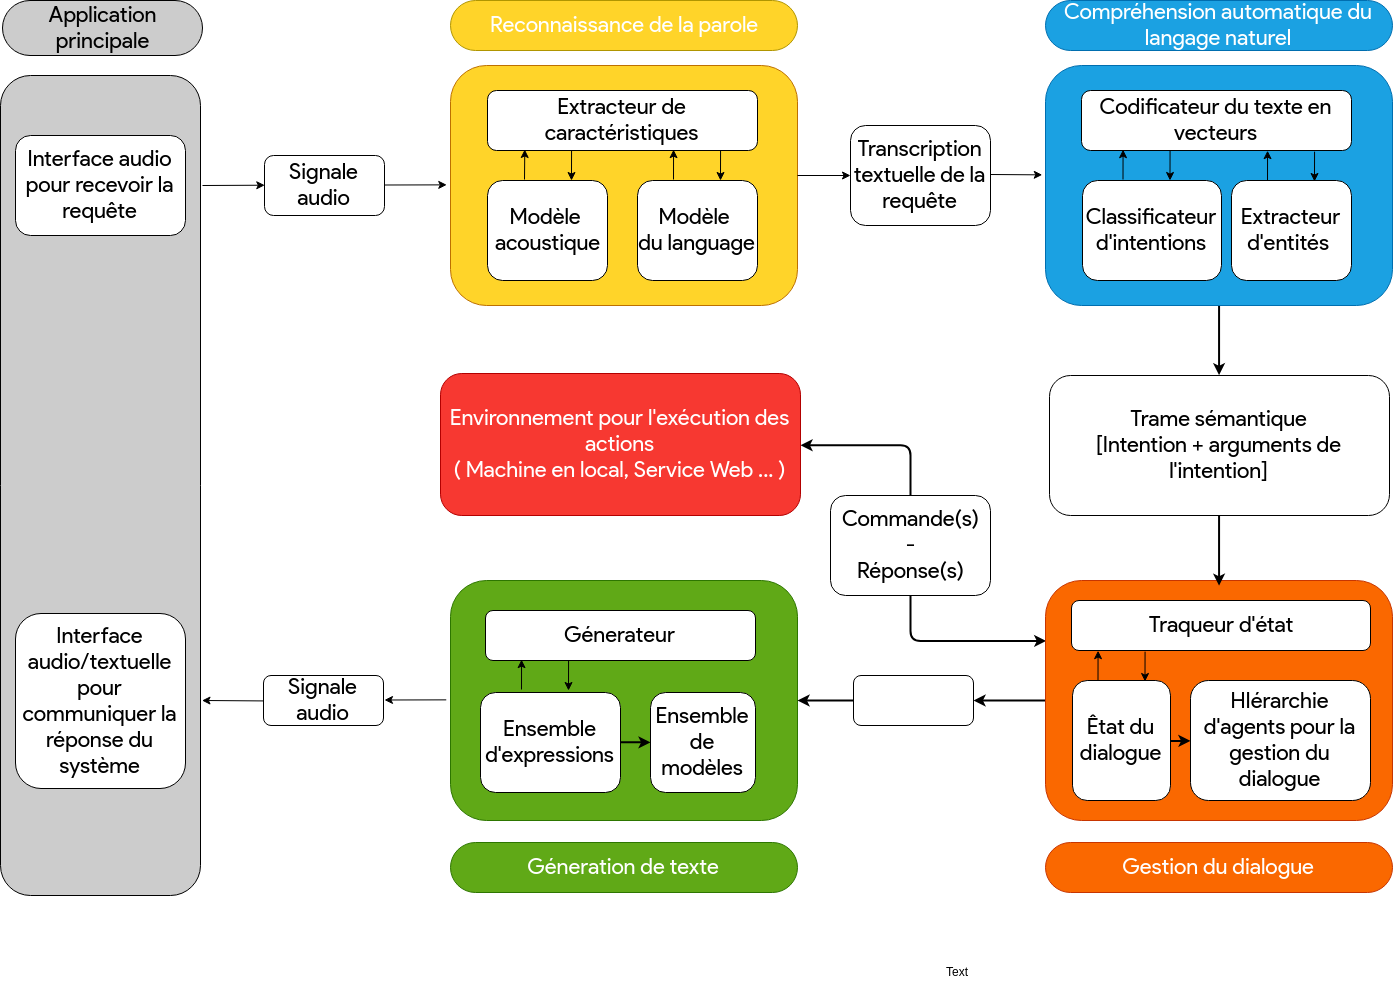
\includegraphics[width=\linewidth]{images/SPA_architecture.png}
	\caption{Architecture générale du système Bethano}
	\label{spaArch}
\end{figure}


	\subsection{Partie utilisateur}
%	What the users sees as input/output and the interfaces that are available for him
	\paragraph{}
	Cette partie représente ce que l'utilisateur peut voir comme entrée/sortie et les interfaces qui lui sont accessibles. Puisque l'assistant est un processus qui communique majoritairement avec l'utilisateur à travers des échanges verbaux, nous avons pensé à implémenter l'interface du système comme un processus qui s'exécute en arrière plan et qui attend d'être activé (pour le moment par un événement physique, c.à.d un clic sur un bouton/icône ou raccourci clavier). L'assistant pourra ensuite répondre en affichant un texte à l'écran qui sera vocalement synthétisé et envoyé à l'utilisateur via l'interface de sortie de son choix. (Afficher le texte et sa transcription vocale pourrait palier à certains manques comme l'absence d'un périphérique de sortie audio.)
	\subsection{Partie interne du système}
	
%	What the users doesn't see and what are the main components of the system
	\paragraph{}
	\label{system_layer}
	Cette partie quant à elle représente ce que l'utilisateur ne voit pas et fait donc partie du fonctionnement interne du système. Elle regroupe les quatre grandes étapes d'un cycle de vie pour une commande reçue de la couche utilisateur. Comme mentionné dans le chapitre précédent (voir \ref{spaLifeCycle}), la requête passe par un module de reconnaissance de la parole, qui traduira en texte le signal audio correspondant à cette dernière. Le module suivant, à savoir le module de compréhension du langage naturel, va extraire l'intention de l'utilisateur et ses arguments (par exemple \textit{"open the home folder"} pourrait donner  une intention dy type  \textit{open\_file\_desire[file\_name="home",parent\_directory="?"]}). Le gestionnaire de dialogue gardera trace de l'ensemble des échanges effectués entre l'utilisateur et l'assistant et essayera d'atteindre le but final de la requête (récente ou ancienne). Pour ce faire, il aura besoin d'interagir avec ce qu'on a appelé un environnement d'exécution, qui peut être la machine où l'assistant réside ou bien une API \footnote{Application Programming Interface ou interface de programmation applicative.} qui aura accès à un service à distance (sur internet par exemple) ou local (dans un réseau domestique). Finalement, une action spéciale qui servira à informer l'utilisateur sera envoyée au module suivant (c.à.d le module de génération du langage naturel) pour être transformée en son équivalant dans un langage naturel, puis le texte sera vocalement synthétisé et envoyé vers l'interface de sortie de l'application.

	\par
	Nous allons maintenant détailler la conception des différents modules en précisant à chaque fois le ou les procédés de sa mise en \oe{}uvre. 
\section{Module de reconnaissance automatique de la parole}
\paragraph{}
\label{asr_probs}
Premier module du système Bethano, le module de reconnaissance automatique de la parole (Automatic Speech Recognition, ASR) joue un rôle clé dans le dialogue entre l'utilisateur et la machine. En effet, il doit être assez robuste et précis dans la transcription de la requête en entrée afin de minimiser les erreurs et les ambiguïtés qui peuvent survenir dans le reste du pipeline. Dans cette optique, nous avons décidé de ne pas développer entièrement un sous-système en partant de zéro; faute de temps et par soucis de précision nous avons opté pour l'exploitation d'un outil open-source nommé DeepSpeech \citep{deepspeech_paper}. Naturellement, du fait que ce soit un projet open-source nous, avons pu avoir accès à différentes informations concernant le modèle d'apprentissage, d'inférence et la nature des données utilisées pour l'apprentissage les tests.
	\subsection{Architecture du module ASR}
	\paragraph{}
	Le module possède une architecture en pipeline dont chaque composant exécute un traitement sur la donnée reçu par son prédécesseur.
	\begin{figure}[H] 
		\centering
		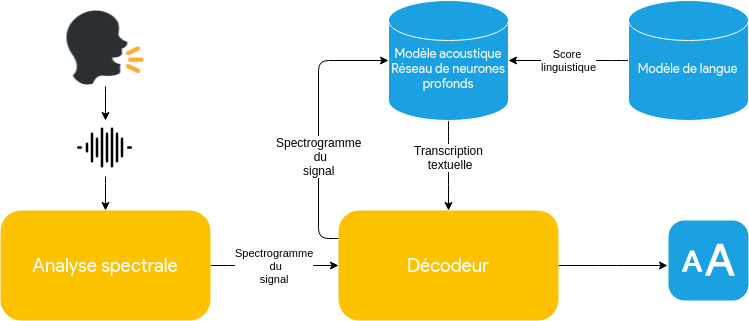
\includegraphics[width=0.88\linewidth]{images/Conception/ASR/schema.png}
		\caption{Architecture du module de reconnaissance de la parole (ASR)}
	\end{figure}
	\subsection{Modèle acoustique}
		\subsubsection*{Type du modèle}
		\paragraph{}
		Le modèle d'apprentissage (qui est principalement le modèle acoustique à l'exception d'une partie consacré au modèle linguistique) possède une architecture en réseau de neurones avec apprentissage de bout-en-bout composé de trois parties : 
		\begin{itemize}
			\item Deux couches de convolution spatiale : pour capturer les patrons dans la séquence du spectrogramme du signal audio.
			\item Sept couches de récurrence (Réseaux de neurones récurrents) pour analyser la séquence de patrons (ou caractéristiques) engendrée par les couches de convolutions. 
			\item Une couche de prédiction utilisant un réseau de neurones complètement connecté pour prédire le caractère correspondant à la fenêtre d'observation du spectrogramme du signal audio. La fonction d'erreur prend en compte la similarité du caractère produit avec le véritable caractère ainsi que la vraisemblance de la séquence produite par rapport à un modèle de langue basé sur les N-grammes (voir \ref{n-grams})
		\end{itemize}
		\begin{figure}[H] 
			\centering
			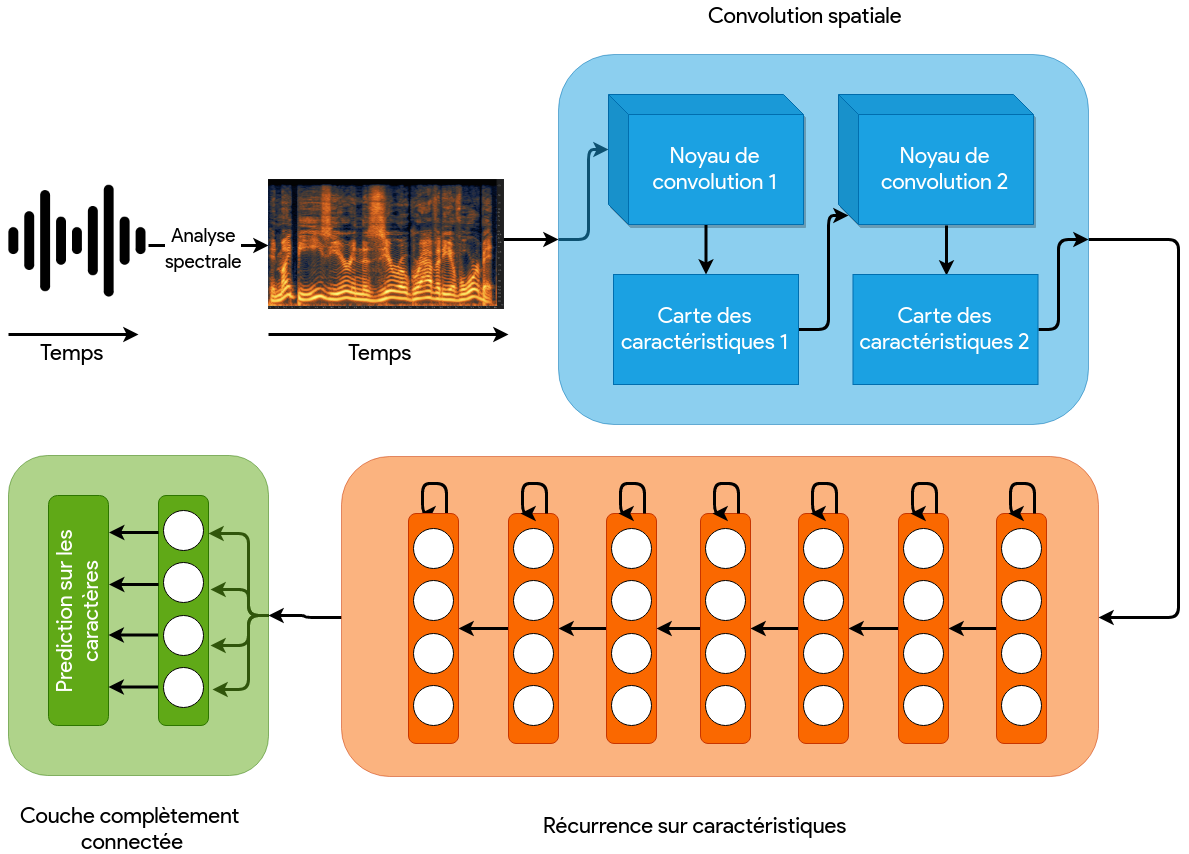
\includegraphics[width=0.88\linewidth]{images/Conception/ASR/deeps_speech_arch.png}
			\caption{Architecture du modèle DeepSpeech \citep{deepspeech_paper}}
			\label{fig:deepSpeechArch}
			
		\end{figure}
		\subsubsection*{Données d'apprentissage}
%		audio files and their transcriptions
		\label{common_voice}
		\paragraph{}
		Pour entraîner le modèle acoustique, Mozilla a lancé le projet Common Voice \footnote{\url{https://voice.mozilla.org/fr}}, une plateforme en ligne pour récolter des échantillons audios avec leurs transcriptions textuelles. Chaque batch (lot) de données reçu est alors manuellement validé par l'équipe de Mozilla pour l'inclure dans la banque de données d'exemples principale. À ce jour, pour la langue anglaise, la plateforme a récolté plus de 22Go de données, soit 803 heures d'enregistrements correspondant à plus de 30 000 voix différentes dont 582 heures ont été validées. Cependant, ce volume de données est relativement petit comparé à celui déjà utilisé pour l'apprentissage initial. En effet, plusieurs sources ont été combinées pour construire cet ensemble de données. Dans \citep{deepspeech_paper} il a été mentionné que trois ensembles d'apprentissage existants ont étés choisis dont WSJ (Wall Stret Journal) \footnote{\url{http://www.cstr.ed.ac.uk/corpora/MC-WSJ-AV/}}, Switchboard \footnote{\url{https://catalog.ldc.upenn.edu/LDC97S62}} et Fisher \footnote{\url{https://catalog.ldc.upenn.edu/LDC2004S13}}, qui à eux trois cumulent 2380 heures d'enregistrements audios en anglais et plus de 27 000 voix différentes. Vient s'ajouter à cela l'ensemble Baidu \footnote{\url{https://ai.baidu.com/broad/introduction}} avec 5000 heures d'enregistrements et 9600 locuteurs.
		
	\subsection{Modèle de la langue}
		\subsubsection*{Type du modèle}
		\paragraph{}
		
		Pour ce qui est du type du modèle de langue, c'est un modèle basé sur les N-grammes (3-grammes pour être plus précis) qui est utilisé. Il permet de façon assez simple et intuitive de capturer l'enchaînement des mots dans une langue donnée, rendant ainsi la transcription finale assez proche de la façon dont les mots sont distribués dans le corpus d'apprentissage.
		
		\subsubsection*{Données d'apprentissage}
		\paragraph{}
		À l'origine, DeepSpeech utilise un modèle de langue dont la source n'est pas dévoilée par les chercheurs dans \citep{deepspeech_paper}, mais son volume est approximativement de 220 million de phrases avec 495 000 mots différents. Cependant, puisque ce corpus nous reste inconnu et qu'il a probablement été construit pour reconnaître des séquence de mots en anglais assez générales, nous avons décidé de construire notre propre modèle de langue en récoltant des données depuis des dépôts sur le site \href{https://github.com/}{Github}, plus précisément les fichiers README.md des dépôts qui font office de manuels d'utilisation d'un projet hébergé sur le site. Ce type de fichiers renferme généralement des instructions de manipulation de fichiers, de lancement de commandes, etc; ce qui offre un bon corpus pour le modèle de langue. En effet notre système se concentre plus sur l'aspect de manipulation d'un ordinateur, donc la probabilité de trouver certaines séquences de mots qui appartiennent au domaine technique	 est en théorie plus élevée. La procédure suivi est la suivante : 
		\begin{figure}[H] 
			\label{fig:lm_gathering}
			\centering
			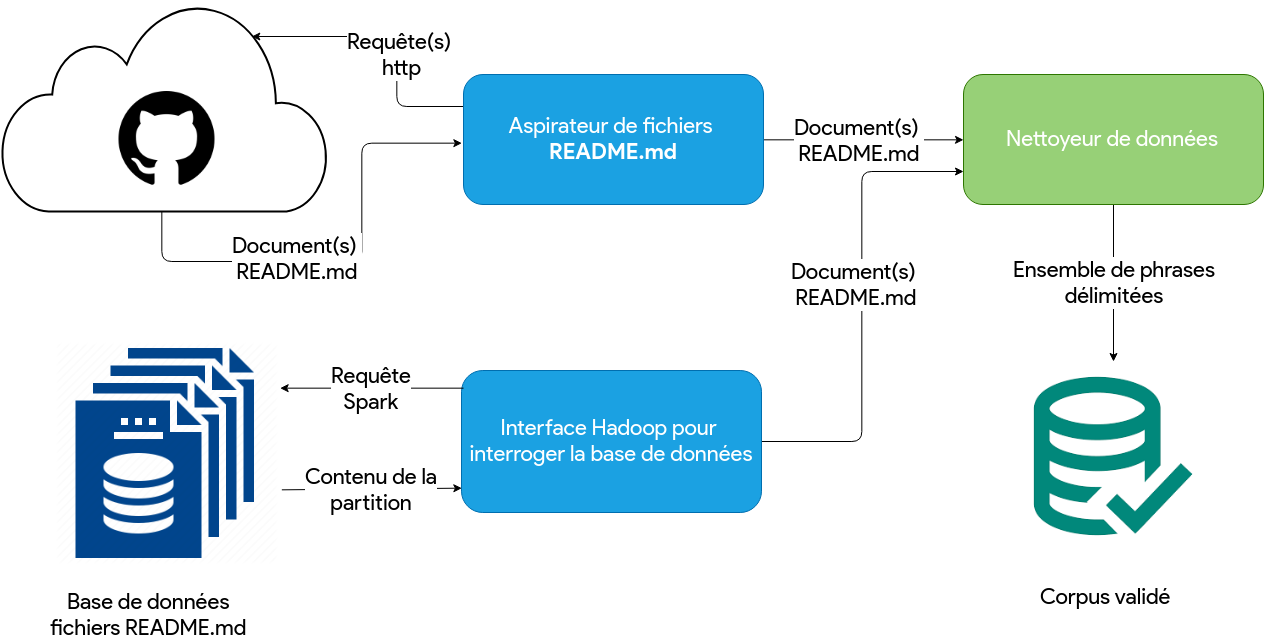
\includegraphics[width=0.88\linewidth]{images/Conception/ASR/lm_gathering.png}
			\caption{Processus de génération du corpus pour le modèle de langue}
		\end{figure}
		\begin{itemize}
			\item L'acquisition des données dans leur format brut \textbf{.md} (markdown) se fait de deux manières :
			\begin{itemize}
				\item Depuis le site officiel de GitHub en faisant des requêtes http au serveur en suivant le patron suivant pour les urls : 
				\begin{lstlisting}[language=python]
				'http://raw.githubusercontent.com/'+NOM_DÉPOT+'/master/README.md'\end{lstlisting}
				La liste des noms de dépôts est disponible dans un fichier \footnote{\url{https://data.world/vmarkovtsev/github-readme-files/file/top_broken.tsv}} en free open acces (accès ouvert et libre) au format \textbf{.csv} dont les colonnes sont \textit{Nom\_Utilisateur} et \textit{Nom\_Dépot} 
				\item En lisant une base de 16 millions de fichiers différents dont la taille totale atteint 4.5 Go  
			\end{itemize}
			\item Les deux sources de données envoient ensuite les fichiers récoltés au nettoyeur de fichiers pour en extraire seulement les parties qui ont du sens dans le langage naturel (paragraphes, titres, instructions, etc.)
			\item Le corpus final est ensuite construit à partir des paragraphes extraits à l'étape précédente après les avoir segmentées en phrases (en utilisant un modèle de segmentation prédéfini) donnant un ensemble de phrases dans format le suivant \begin{lstlisting}[language=xml]
			<s>select and click edit</s>
			<s>browse to demo on your web browser</s>
			...
			<s>you can specify these values in a file that file must be hom</s>\end{lstlisting}
		\end{itemize}
	

\section{Module de compréhension automatique du langage naturel}
\paragraph{}
Second module du système, le module de compréhension automatique du langage naturel (Natural Langage Understanding, NLU) à pour rôle de faire office de couche d'abstraction entre la requête de l'utilisateur (formulée dans un langage naturel) et le fonctionnement interne du système qui communique à travers un langage plus formel. On parle ici de la construction d'une représentation sémantique de la requête. Pour ce faire nous avons opté pour l'approche par apprentissage automatique, compte tenu des bons résultats obtenus par certaines architectures ( \citep{intent_slots},\citep{intent_classification}) et cela malgré le petit volume des données d'apprentissage. Cette option nous a paru plus abordable que la construction d'un analyseur basé règles, souvent assez rigide et dont l'exhaustivité n'est pas évidente à obtenir.
	\subsection{Architecture du module}
	\begin{figure}[H] 
		\label{nlu_arch}
		\centering
		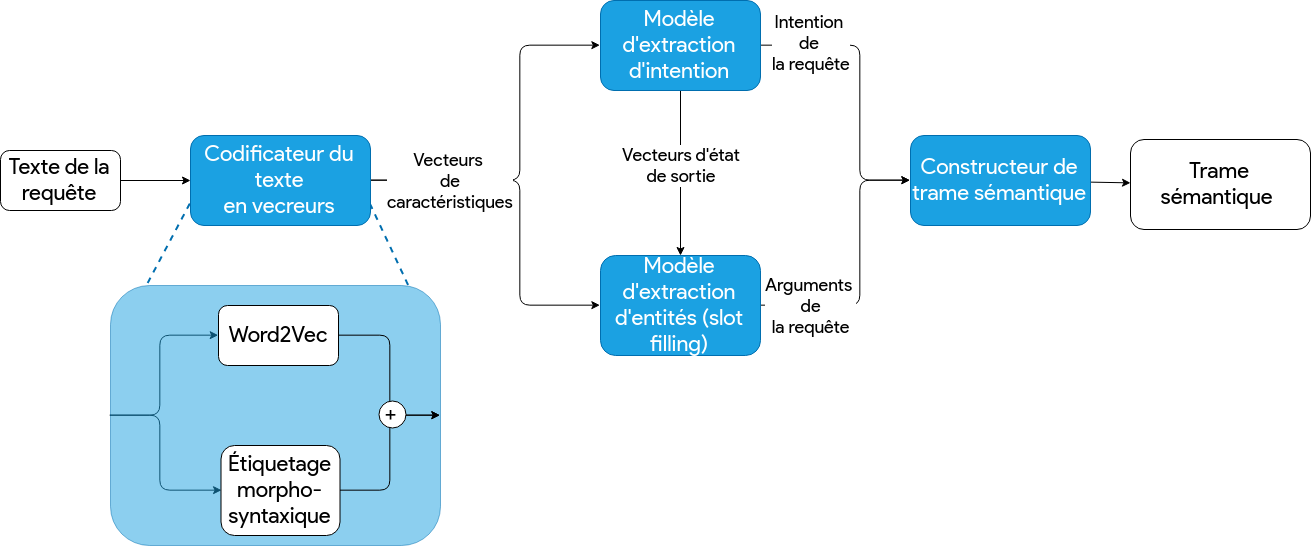
\includegraphics[width=\linewidth]{images/Conception/NLU/nlu_module_arch.png}
		\caption{Architecture du module de compréhension automatique du langage naturel (NLU)}
	\end{figure}
	\paragraph{}
	\label{encoding}
	Comme précédemment cité (voir la \ref{system_layer}), le module NLU possède une architecture en pipeline qui reçoit en entrée le texte brut de la requête. Sa codification varie selon les approches que nous avons explorées et qui seront plus explicitées dans le chapitre suivant Réalisation et résultats. Pour mieux capturer l'aspect sémantique des mots dans le texte, nous avons décidé d'utiliser le modèle Word2Vec pré-entraîné par Google (entraîné sur 100 milliard de mots) pour produire un vecteur de taille fixe pour chaque mot. Pour encoder l'information syntaxique de la requête nous avons concaténé au vecteur de prolongement de chaque mot de la requête (Word Embedding Vector) le vecteur codifiant son étiquette morphosyntaxique. Après avoir codifié la séquence de mots, elle est envoyée aux modèles de classification d'intentions et d'extraction d'entités \footnote{Par entité nous entendons les arguments de l'intention.}, qui sont en fait un seul modèle joint dont l'architecture est détaillée dans la section \ref{joint_model}. Ces deux informations sont ensuite décodées et passées au constructeur de trame sémantique qui structurera ces dernières en une seule entité sémantique dans le format suivant : 
	\newpage
	\begin{lstlisting}[language=json]
	{
		intent  : "open_file_desire",
		entities : [
			{	
				entity	: "string",
				name	: "file_name",
				value	: "test.py",
				start	: "31",
				end		: "37",
			}
		]
	}
	\end{lstlisting}
	\par
	Une trame sémantique se compose de deux parties :
	\begin{itemize}
		\item \textbf{Partie intentions} : l'intention extrait à partir de la requête. Elle se trouvera dans l'entrée $"intent"$ de la trame.
		\item \textbf{Partie arguments} : aussi appelées entités du domaine, ces arguments sont extrait depuis le texte de la requêtes. L'entrée $entities$ contient une liste d'arguments. chaque élément de la liste renseigne sur le type, le nom, la valeur et l'emplacement d'une entité.
	\end{itemize}
%	\subsection{Analyse sémantique basée sur les grammaires de dépendances}
	\subsection{Analyse sémantique avec apprentissage automatique}
		\subsubsection{Modèle(s) utilisé(s)}
		\paragraph{}\label{joint_model}
		Comme vu dans le chapitre précédent (voir \ref{nlu_chap2}) l'architecture adoptée est une architecture mono-entrée/multi-sorties dont l'entrée est une séquence de mots codifiés et les sorties sont une séquence d'étiquettes et ainsi qu'une classe associée au texte. Nous pouvons distinguer les deux parties qui sont l'encodage et le décodage de la séquence. 
		\par L'encodage sert à la fois à l'attribution de la classe (l'intention) et à l'initialisation de la séquence de décodage (pour l'attribution d'une étiquette à chaque mot).
		Il se fait en utilisant un réseau de neurones récurrent de type B-LSTM (Bidirectionall Long Short Term Memory) pour mieux capturer le contexte droit (respectivement gauche) de chaque entrée selon le sens de traitement des données dans le réseau B-LSTM. Le dernier vecteur en sortie est ensuite utilisé comme vecteur d'entrée pour un réseau de neurones Fully Connected (Complètement connecté) dont la dernière couche est une couche de prédiction sur une distribution de probabilités des intentions possibles.
		\par
		Le décodeur est aussi un réseau de neurones récurent de type B-LSTM. Il prend en entrée le vecteur précédemment retourné par l'encodeur, ainsi, à chaque étape de l'inférence une étiquette est produite en sortie pour chaque position du texte en entrée (les longueurs des séquences d'entrée et de sortie sont donc identiques) en utilisant un autre réseau de neurones Fully Connected sur chaque vecteur d'état de sortie des cellules LSTM du décodeur (voir la figure ~\ref{fig:lstmslots}).
		\subsubsection{Les données d'apprentissage}
		\paragraph{}
		\label{nlu_dataset}
		Ne disposant pas d'un ensemble d'apprentissage pré-existant pour les intentions que nous avons développées, nous avons tenté d'en construire un nous-mêmes en l'enrichissant avec quelque modifications. Dans \citep{rasa_nlu} il a été noté que pour une tâche assez simple (comme pour notre cas l'exploration des fichiers dans un premier temps) il n'est pas nécessaire de disposer d'une grande quantité de données (une cinquantaine d'exemples par intention approximativement) si les exemples ne sont pas facilement confondus, et surtout si l'espace des possibilité pour les requête est assez réduit et peut facilement être explicitepr. En jouant sur l'ordre des mots nous avons pu générer pour les 15 intentions, 4157 patrons d'exemple au total dont 870 sont dépourvus d'arguments. Un patron d'exemple est une structure contenant des placeholders (compartiments) pouvant être remplis avec des valeurs générées programmatiquement. Par exemple : 
		\begin{lstlisting}[language=json]
		delete the {file_name:} file under {parent_directory:}\end{lstlisting}
		Ces placeholders servent à la fois à générer plus d'exemples mais aussi à étiqueter le texte en chosifiant les valeurs de ces variables comme valeur de l'étiquette. Un exemple d'une entrée de l'ensemble d'apprentissage avant affectation des variables est le suivant : 
		\begin{lstlisting}[language=json]
		
		{
			"id": 6,
			"text": "I want to open the {file_name:} folder",
			"intent": "open_file_desire"
		},
		\end{lstlisting}
		Pour remplir l'ensemble des placeholders, nous commençons d'abord par scanner le répertoire de la machine avec une profondeur max (c.à.d les niveaux de répertoires et sous-répertoires) égale à 5. Nous avons aussi ajouté une liste\footnote{\url{https://github.com/xmendez/wfuzz/blob/master/wordlist/general/common.txt}} des noms de fichiers et répertoires les plus populaires.
		Les noms des répertoires sont ensuite nettoyés à l'aide d'expressions régulières et transformés en un format universel établi à l'avance \textbf{nom\_du\_fichier} en choisissant "\_" (le tiret du 8) comme séparateur. En bouclant sur ces noms de répertoire nous pourrons donc construire plusieurs exemples comme une entrée dans un dictionnaire dont le format est le suivant : 
		\begin{lstlisting}[language=json]
		{
			'id': 79372,
			'intent': 'delete_file_desire',
			'postags': ['NN', 'VB', 'DT', 'NN', 'VBN', 'NN', 'NNS'],
			'tags': 'NUL NUL NUL NUL NUL ALTER.file_name ALTER.file_name',
			'text': 'please remove the file named platform notifications'
		}
		\end{lstlisting}
		\par
		\newpage
		Une entrée est divisée en cinq champs :
		\begin{itemize}
			\item \textbf{id} : un entier qui sert d'identificateur pour l'instance.
			\item \textbf{intent} : l'intention (non encore codifiée) attribuée à l'instance.
			\item \textbf{tags} : les étiquettes de chaque mots de la requête, une étiquette peut être soit $NUL$ (ce n'est pas un argument) ou bien le nom de l'entité (argument) que représente le mot à la position étiquetée. La liste complète des intentions avec leurs arguments se trouve dans le tableau \ref{tab:all_intents} du chapitre Réalisation et résultats.
			\item \textbf{postags} : la liste des étiquettes morphosyntaxiques de chaque mots de la requête. L'ensemble des étiquettes utilisées est celui du Penn Treebank \citep{penn_treebank}.
			\item \textbf{text} : le texte de la requête nettoyé et dont les mots sont séparés uniquement par un espace.
		\end{itemize}
\section{Module de gestion du dialogue}
Le but de ce module est de décider quelle action prendre à chaque instant du dialogue. De prime abord nous allons présenter l'architecture globale de ce module notamment la représentation des informations reçues et la politique d'actions. Ensuite, nous allons détailler la conception de chaque partie.
\subsection{Architecture du module}
Comme nous avons déjà vu, l'architecture typique des gestionnaires de dialogue se compose de deux parties principales: 
\begin{itemize}
	\item Un module qui suit l'état du dialogue: Pour gérer le dialogue avec l'utilisateur, le gestionnaire doit représenter l'état du dialogue de façon à pouvoir répondre aux actions de l'utilisateur. Ce module sert à suivre cet état après chaque étape du dialogue.
	\item Une politique d'actions: Celle-ci détermine l'action à prendre à partir d'un état donné.
\end{itemize}
\subsubsection{État du dialogue}
Avant de détailler les deux modules du gestionnaire. Il est nécessaire d'introduire une représentation de l'état du dialogue. Classiquement, les trames sémantiques ont été utilisées dans ce but (voir \ref{trame}). Le suivi d'état se fait dans ce cas en gardant trace des emplacements remplis durant le dialogue.
Nous avons opté pour l'utilisation d'une représentation plus riche, les graphes de connaissances, qui sont une forme de représentation où les connaissances sont décrites sous forme d'un graphe orienté étiqueté. Des travaux ont déjà utilisé des graphes de connaissances \citep{Stoyanchev2018} et des ontologies \citep{Wessel2019} pour représenter l'état du système de dialogue. À partir de ce dernier une base de règles décide quelle action prendre directement du graphe. L'avantage d'utiliser des graphes de connaissances par rapport à l'utilisation des trames sémantiques apparaît dans leur flexibilité et leur dynamisme. En effet, pour une tâche comme la navigation dans les fichiers, l'état de l'arborescence des fichiers est sujet à des changements fréquents: ajout, suppression, modification, etc. Il est difficile de faire une représentation de l'information dans ce cas avec de simples emplacements à remplir.
\subsubsection{Suivi de l'état du dialogue}
Le rôle du premier module est de mettre à jour l'état du système au cours du dialogue. Il reçoit l'action de l'utilisateur ou du gestionnaire et il produit un nouvel état. Dans notre cas, le module NLU produit toujours une trame sémantique contenant l'intention de l'utilisateur ainsi que ses paramètres. C'est alors le travail du traqueur d'état d'injecter le résultat du module NLU dans le graphe de connaissances. Ceci consiste à transformer la trame sémantique en un graphe qui est ensuite ajouté au graphe d'états. Plus de détails seront donnés dans la section \ref{onto} où nous construirons une ontologie pour définir un vocabulaire de dialogue et comment elle peut être utilisée pour passer du résultat du module NLU en un graphe de connaissances.
\begin{figure}[H] 
	
	\centering
	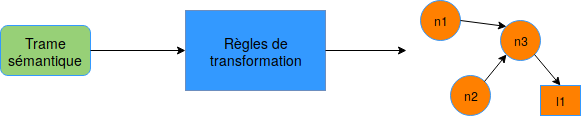
\includegraphics[width=0.8\linewidth]{images/Conception/DM/Transformer.png}
	\caption{Schéma de transformation de trame sémantique en graphe}
\end{figure}\label{transformer}
\subsubsection{La politique d'actions}
La politique d'actions peut être écrite manuellement, apprise à partir d'un corpus ou à l'aide de l'apprentissage par renforcement. Dans ce dernier cas, un agent doit interagir avec un utilisateur qui évalue ses performances afin qu'il puisse apprendre. Étant donné que l'apprentissage par renforcement nécessite un nombre important d'interactions, il est primordial d'utiliser un simulateur d'utilisateur. Ce dernier peut être à base de règles, ou un modèle statistique extrait à partir d'un corpus de dialogue.
\par Dans les trois cas de figure, il est difficile de réaliser un modèle varié et qui peut accomplir plusieurs tâches. D'un coté, un corpus contenant des dialogues sur toutes les tâches possibles est difficile à acquérir, si ces derniers sont nombreux et spécifiques à une application précise. De l'autre coté, écrire les règles d'un système de dialogue ou d'un simulateur d'utilisateur s'avère compliqué et nécessite un travail manuel énorme pour gérer toutes les tâches possibles.
\par Pour pallier à cela, nous proposons d'utiliser une architecture multi-agents hiérarchique dans laquelle les agents feuilles sont des agents qui peuvent répondre à une tâche ou une sous-tâche bien précise, tandis que les agents parents sélectionnent l'agent fils capable de répondre à l'intention de l'utilisateur.
\begin{figure}[H] 
	
	\centering
	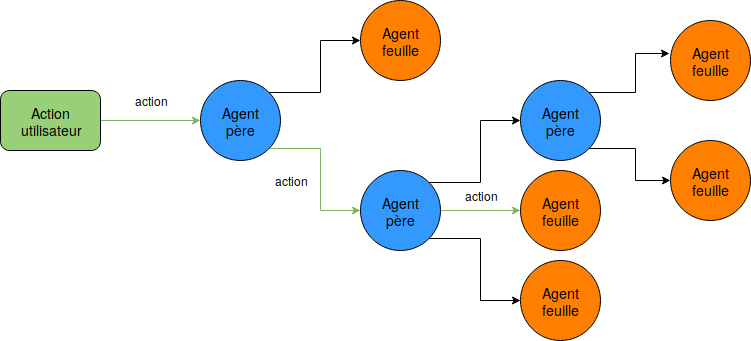
\includegraphics[width=0.8\linewidth]{images/Conception/DM/multiagent.png}
	\caption{Schéma de l'architecture multi-agents pour la gestion du dialogue}
\end{figure}\label{multiagent}
L'avantage de l'architecture multi-agents hiérarchique est de permettre la division du problème en plusieurs sous-problèmes indépendants. En effet, un simulateur d'utilisateur ou un corpus qui sont destinés pour une seule tâche sont considérablement plus abordables à créer. De plus, cette architecture permet un développement incrémental dans le sens où elle facilite l'addition d'une nouvelle tâche pour l'assistant; il suffit d'ajouter des agents capables de traiter cette nouvelle tâche à l'architecture. Cependant, un travail supplémentaire s'avère nécessaire qui est celui des agents parents. Ce travail est relativement simple; il suffit de faire un apprentissage supervisé des agents parents avec les simulateurs d'utilisateurs des agents fils. À tour de rôle et avec des probabilités de transitions entre les simulateurs d'utilisateurs, ces derniers communiquent avec l'agent parent. Comme on connaît pour chaque simulateur l'agent fils qui lui correspond, il est donc possible de faire un apprentissage supervisé où les entrées sont les actions des simulateurs et l'état du système, tandis que la sortie est l'agent fils qui peut répondre à l'action.
\begin{figure}[H] 
	
	\centering
	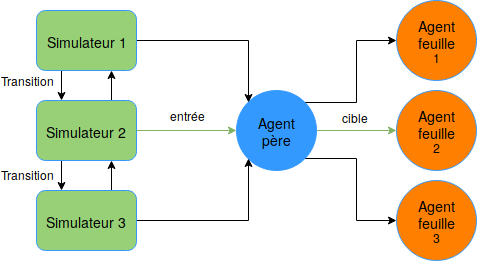
\includegraphics[width=0.5\linewidth]{images/Conception/DM/train_parent.png}
	\caption{Schéma représentant l'apprentissage des agents parents avec les simulateurs des agents feuilles}
\end{figure}\label{train_parent}
\paragraph{}
Pour résumer l'architecture globale du gestionnaire de dialogue, lorsqu'une nouvelle action utilisateur arrive au système, le traqueur d'état la reçoit et met à jour l'état du système en transformant l'action en un graphe de connaissances pour l'ajouter au graphe d'état. Ce nouveau graphe d'état ainsi que la dernière action reçue sont transmis à une architecture multi-agents hiérarchique qui va décider quelle action le système de dialogue doit prendre.
\begin{figure}[H] 
	
	\centering
	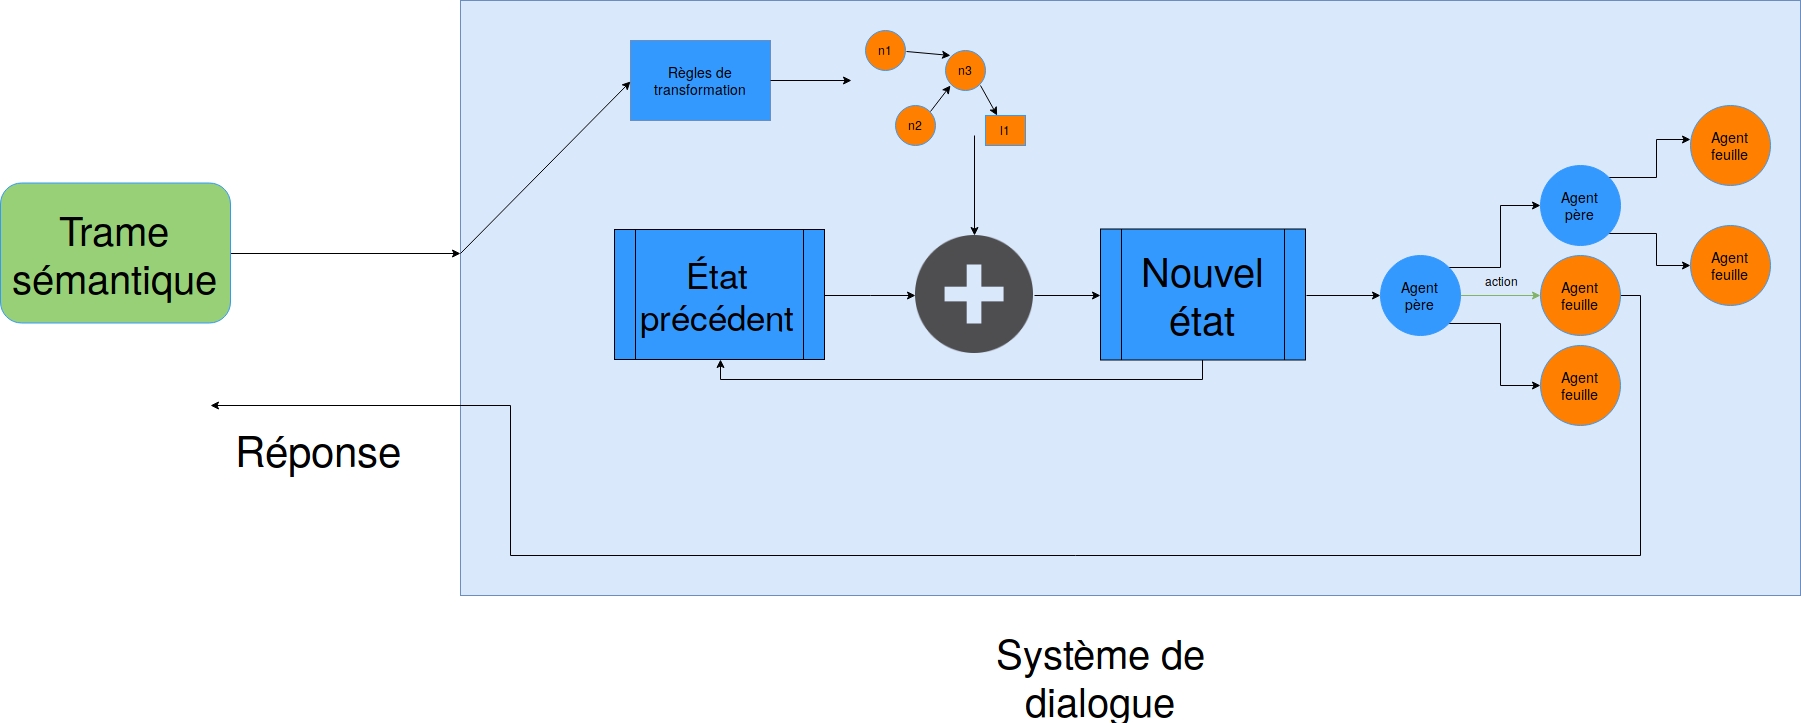
\includegraphics[width=0.88\linewidth]{images/Conception/DM/globalDM.png}
	\caption{Schéma global du gestionnaire de dialogue}
\end{figure}\label{globalDM}
\subsection{Les ontologies du système}\label{onto}
\paragraph{}Une ontologie est une représentation des concepts et des relations d'un domaine donné. Elle définit un vocabulaire pour ce domaine afin de permettre aux programmes intelligents de comprendre  et de communiquer sur des données reliées à ce domaine.
\par Nous définissons une ontologie de dialogue ainsi que des ontologies pour chaque tâche réalisable par notre assistant. Ceci permettra à notre gestionnaire de comprendre le dialogue et les tâches qu'il peut réaliser.
\subsubsection{Ontologie de dialogue}\label{onto1}
Nous définissons en premier une ontologie de dialogue qui contient des concepts qui peuvent aider un assistant d'ordinateur à gérer son dialogue.
\begin{figure}[H] 
	
	\centering
	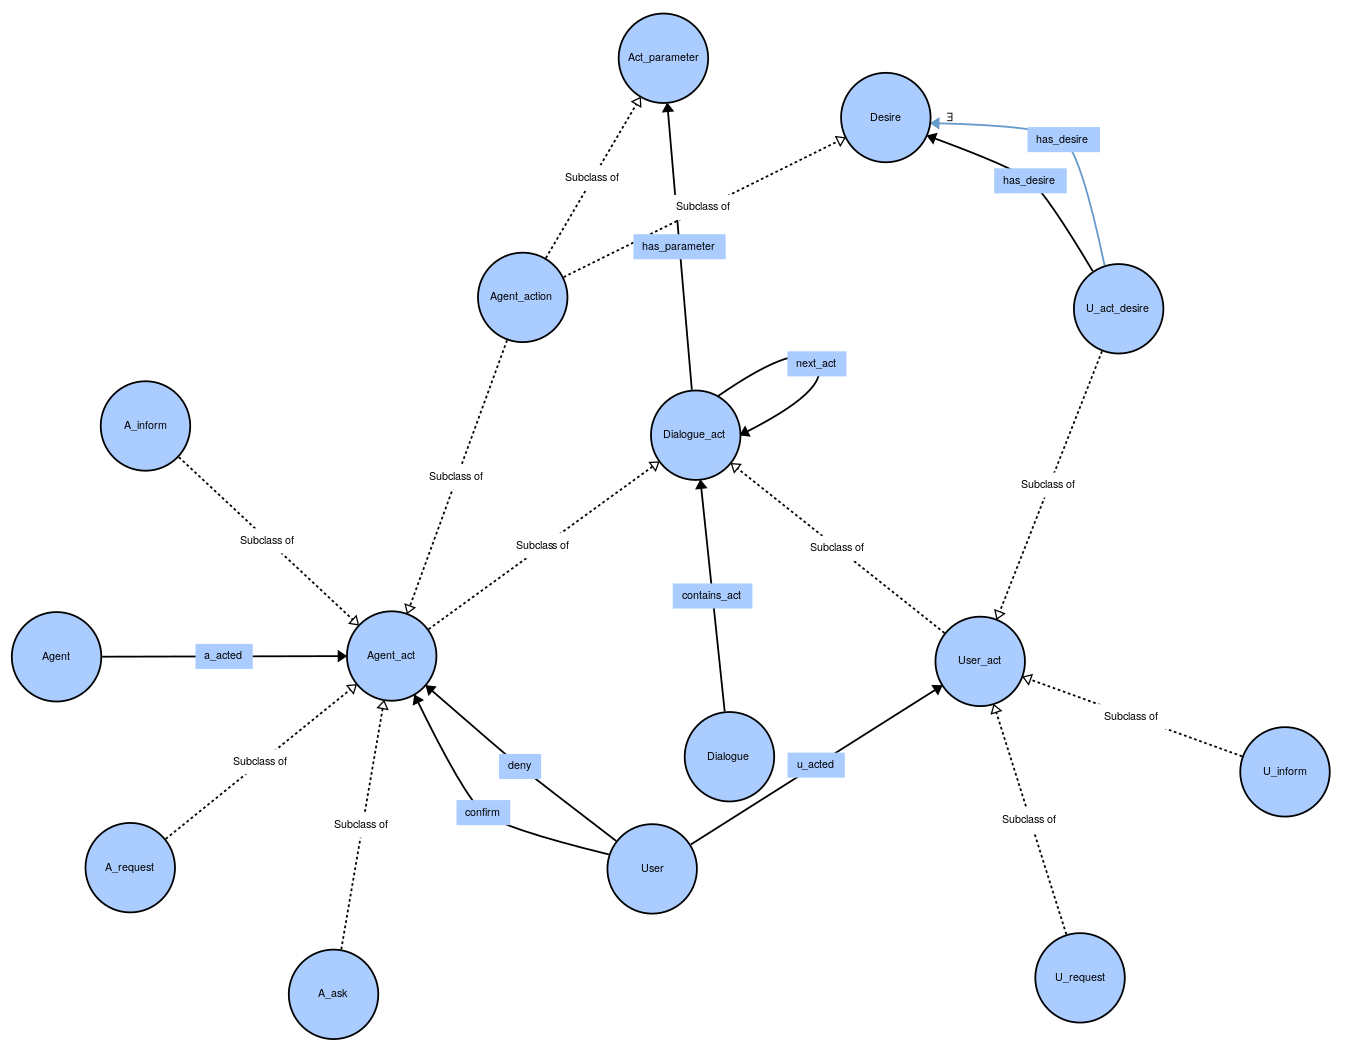
\includegraphics[width=1.1\linewidth]{images/Conception/DM/main_onto.png}
	\caption{Graphe de l'ontologie de dialogue}
\end{figure}\label{mail_onto}
Principalement l'ontologie se compose de six classes mères:
\begin{itemize}
	\item $Agent$ et $User$: ce sont les classes qui représentent l'utilisateur et l'agent qui participent au dialogue.
	\item $Dialogue$: l'agent et l'utilisateur participent à un dialogue; ce dernier contient les actions des deux participants.
	\item $Dialogue\_act$: il s'agit de la classe qui représente une action du dialogue, elle a deux sous-classes $Agent\_act$ et $User\_act$ qui représentent les actions de l'agent et de l'utilisateur respectivement.
	\item $Act\_parameter$: C'est la classe mère des paramètres que peuvent prendre les actions de dialogue. Par exemple, l'action d'informer peut avoir comme paramètre le nom d'un fichier.
	\item $Desire$: C'est la classe mère des actions de l'agent que l'utilisateur peut demander. Par exemple, il peut demander l'ouverture d'un fichier donné.
\end{itemize}
Le reste des classes sont des classes filles qui détaillent plus les concepts du dialogue agent-utilisateur.
\par À l'arriver d'une nouvelle action, le traqueur d'état va créer le graphe correspondant. Un exemple abstrait de cela est représenté dans la figure \ref{abstract_onto}. Une nouvelle action utilisateur est créée ainsi que ses paramètres et les relations entre eux.
\begin{figure}[H] 
	\centering
	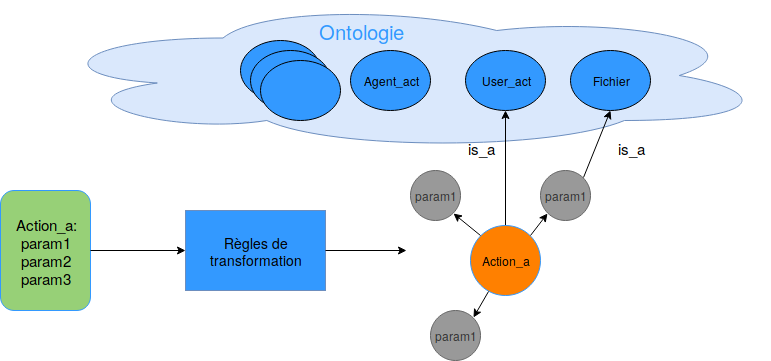
\includegraphics[width=0.88\linewidth]{images/Conception/DM/abstract_onto.png}
	\caption{Schéma de transformation d'une action en graphe}\label{abstract_onto}
	
\end{figure}
\subsubsection*{Ontologie pour l'exploration de fichiers}\label{onto2}
Un exemple d'ontologie pour la compréhension d'une tâche réalisable par l'assistant est celle de l'exploration de fichiers.
\begin{figure}[H] 
	
	\centering
	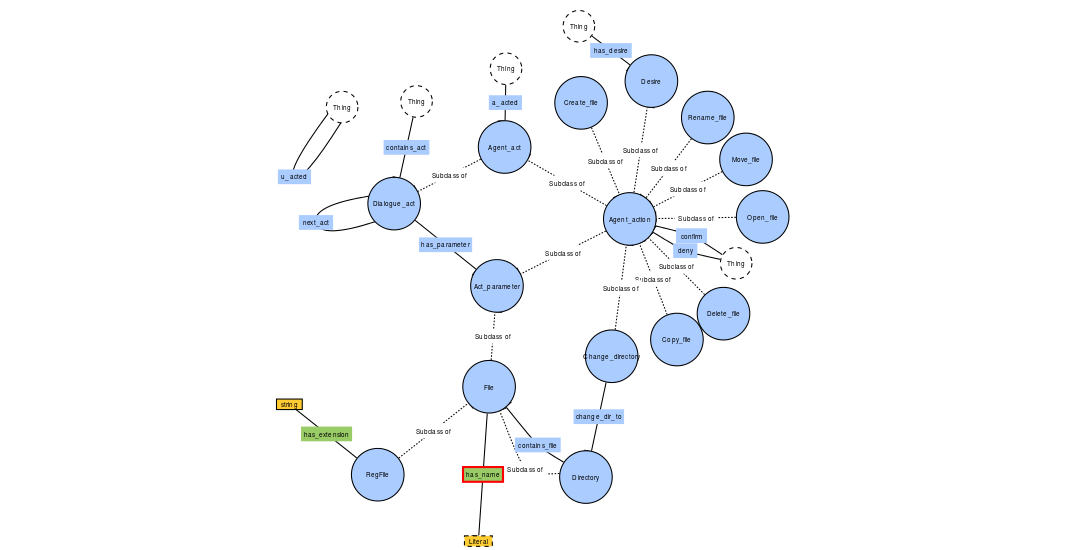
\includegraphics[width=1.1\linewidth]{images/Conception/DM/onto_browser.png}
	\caption{Graphe de l'ontologie de l'exploration de fichiers}
\end{figure}\label{onto_browser}
L'ontologie contient essentiellement:
\begin{itemize}
	\item Des actions sur les fichiers: Créer un fichier, supprimer un fichier, changer de répertoire, etc. Ces actions sont des sous-classes de la classe  $Agent\_act$ vue précédemment ainsi que les classes $Act\_parameter$ et $Desire$. Ceci veut dire, d'un côté, que ces actions peuvent être des paramètres d'autres actions, comme "demander à l'utilisateur s'il veut que l'assistant réalise une action donnée" et d'un autre côté, que l'utilisateur peut demander à l'assistant d'effectuer une de ces actions. 
	\item Les concepts qui sont liés à l'exploration de fichiers sont des sous-classes de $Act\_parameter$ étant donné qu'ils peuvent  être des paramètres d'actions. Par exemple, l'action d'ouvrir un fichier a comme paramètre un fichier.
	\item Des relations entre concepts sont aussi définies. Par exemple, un répertoire peut contenir des fichiers, ou une action de changement de répertoire doit avoir comme paramètre un répertoire cible.
\end{itemize}
La figure \ref{nonabstract_onto} représente l'arrivé d'une nouvelle action: "créer un fichier nommé 'travail'". L'action de l'utilisateur est donc représentée par un nouveau n\oe{}ud de type $U\_act\_desire$ qui désigne une action utilisateur qui demande une action de l'assistant. Cette dernière a comme paramètre un n\oe{}ud de type $Create\_file$ qui est l'action de l'agent que l'utilisateur veut réaliser. Cette action à son tour a des paramètres comme, dans ce cas, le fichier qu'on veut créer.
\begin{figure}[H] 
	\centering
	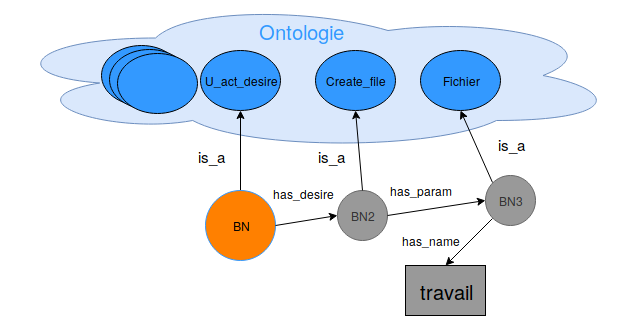
\includegraphics[width=0.88\linewidth]{images/Conception/DM/nonabstract_onto.png}
	\caption{Schéma de transformation d'une action de demande de création de fichier en graphe}\label{nonabstract_onto}
	
\end{figure}
Similairement, les graphes des autres actions sont créées en se basant sur des règles de transformation.
\subsection{Les simulateurs d'utilisateurs}
Plusieurs méthodes peuvent être utilisées pour la création de simulateurs d'utilisateurs (voir \ref{usersim}). Les simulateurs basés sur des méthodes d'apprentissage sont les plus robustes. Cependant, ils nécessitent un nombre important de données. L'alternative c'est d'utiliser des simulateurs basés règles. Nous nous sommes inspirés des simulateurs basés agenda \citep{Schatzmann2007} qui sont des variantes des simulateurs basés règles pour créer nos propres simulateurs. Leur fonctionnement est simple. Ils commencent par générer un but. Pour y arriver, un agenda est créé, qui contient les informations que doit convoyer le simulateur ainsi que les informations qu'il doit recevoir. Les actions sont sélectionnées en suivant des probabilités conditionnelles sur l'état de l'agenda. Enfin, les récompenses sont en fonction des informations reçues de l'agent.
\subsubsection*{Simulateur pour l'exploration de fichiers}
L'exploration de fichiers ne dépend pas de simples informations à transmettre et d'autres à recevoir comme dans les cas d'envoyer un e-mail, chercher une information sur internet ou bien lancer de la musique. Il s'agit d'une tâche dynamique dont la situation de départ est variante. Pareillement, le nombres d'actions change d'un état à un autre. Par exemple, le nombre de fichiers qu'on peut supprimer ou le nombre de répertoires auxquels on peut accéder ne sont pas fixes.
\par Le simulateur commence d'abord par générer une arborescence aléatoire qui représente la situation initiale du système. Ensuite, il duplique cette arborescence en y introduisant des modifications pour générer une arborescence but. Enfin, le simulateur essaye de guider l'agent pour arriver au but en utilisant les actions utilisateurs possibles.
\par En plus des actions de création et suppression de fichiers ainsi que les changements de répertoires qui peuvent guider l'agent au but, d'autres sous-buts peuvent être créés suivant une distribution de probabilité comme copier ou changer l'emplacement d'un fichier, renommer un fichier, ouvrir un fichier etc. Dans ce cas, le simulateur donne la priorité aux sous-buts avant de reprendre les actions menant au but final.
\par L'algorithme suivi par le simulateur est le suivant:
\makeatletter
\def\BState{\State\hskip-\ALG@thistlm}
\makeatother

\begin{algorithm}[H]
	\caption{Algorithme simulateur}\label{euclid}
	\begin{algorithmic}[1]
		\Procedure{Step}{entrées: \textit{action\_agent, max\_tour, tour}; sorties: \textit{recompense, fin, succes, tour}}
		\State $tour \gets tour+1$
		\If {$tour > max\_tour$} 
		\State $fin \gets \textit{true}$
		\State $succes \gets \textit{echec}$
		\State $reponse\_utilisateur \gets $ \textbf{réponse\_fin()}
		\Else
		\State $succes \gets$ \textbf{maj\_état(}$action\_agent$\textbf{)}
		\If {$succes$}
		\State $fin \gets \textit{true}$
		\State $reponse\_utilisateur \gets $ \textbf{réponse\_fin()}
		\Else 
		\State $reponse\_utilisateur \gets $ \textbf{décider\_action(}$action\_agent$\textbf{)}
		\EndIf
		\EndIf
		\State $recompense \gets $\textbf{calculer\_récompense(}$action\_agent, succes$\textbf{)}\\
		\Return $reponse\_utilisateur$
		\EndProcedure
		
	\end{algorithmic}
\end{algorithm}
\begin{itemize}
	\item \textbf{ligne 1:} en entrée de la procédure:
	\begin{itemize}
		\item $action\_agent$: l'action pour laquelle l'agent attend une réponse du simulateur.
		\item $max\_tour$: le nombre maximum d'échanges agent-simulateur.
		\item $tour$: le numéro de l'échange actuel.
	\end{itemize}
	en sortie de la procédure:
	\begin{itemize}
		\item $recompense$: la récompense que donne le simulateur suite à la dernière action de l'agent.
		\item $fin$: un booléen qui détermine si la discussion est terminée.
		\item $succes$: un booléen qui détermine si l'agent est arrivé à un succès.
		\item $tour$: la variable $tour$ est modifiée à l'intérieur de la procédure, elle doit être donc mise en sortie aussi.
	\end{itemize}
	\item \textbf{lignes 3-6:} si le nombre de tours passés est supérieur au nombre maximal de tours autorisés, le simulateur retourne un état d'échec et une action indiquant la fin de la discussion à l'agent.
	\item \textbf{ligne 8:} en mettant à jour l'état du simulateur, ce dernier peut savoir si l'action de l'agent permet d'arriver au but du simulateur.
	\item \textbf{lignes 9-11:} si c'est le cas, le simulateur l'indique à l'agent avec une action de fin et un état de succès.
	\item \textbf{ligne 13:} sinon, le simulateur décide quelle action prendre selon l'action de l'agent. Le diagramme \ref{action_diag} résume cette décision.
\end{itemize}

\begin{figure}[H] 
	\centering
	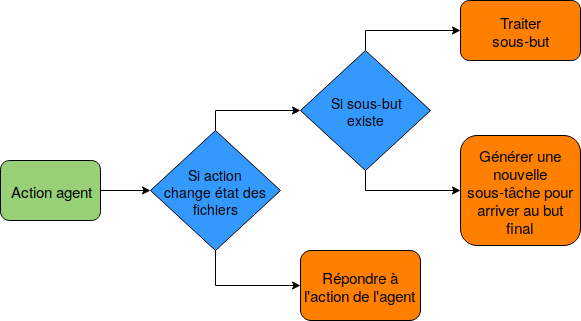
\includegraphics[width=0.88\linewidth]{images/Conception/DM/action_diag.png}
	\caption{Diagramme de décision de l'action à prendre}\label{action_diag}
	
\end{figure}
En ce qui concerne la fonction de récompense, celle-ci est évaluée à partir des changements effectués sur l'état de l'utilisateur. Le tableau \ref{table_reward} associe les changements avec leurs récompenses:
\begin{table}[H]
	\begin{center}
		
		\begin{tabular}{|l|c|} % <-- Alignments: 1st column left, 2nd middle and 3rd right, with vertical lines in between
			\hline
			\textbf{Événements} & \textbf{Récompenses}\\
			\hline
			Similarité améliorée & 2\\
			\hline
			Succès & 2\\
			\hline
			Sous-but réalisé & 2\\
			\hline
			Similarité diminuée & -3\\
			\hline
			Confirmation d'une question & 0\\
			\hline
			Autre & -1\\
			\hline
		\end{tabular}
		\caption{Tableau des récompenses}\label{table_reward}
	\end{center}
\end{table}
\par Il existe deux types d'actions:
\begin{itemize}
	\item Les actions qui affectent l'arborescence de fichiers. Soit elles permettent d'arriver à un sous-but ou bien elles changent la similarité entre l'arborescence courante et l'arborescence du but final.
	\item Le reste des actions sont des échanges agent-utilisateur pour transmettre et recevoir des informations. Par exemple, l'agent peut demander le nom du répertoire parent d'un fichier.
\end{itemize}
\begin{itemize}
	\item Nous avons choisi de donner une récompense unitaire négative pour chaque échange qui n'affecte pas l'arborescence de fichiers. La récompense négative permet d'éviter que le dialogue dure longtemps. L'agent essaye donc de minimiser ce type d'actions afin de ne pas cumuler les récompense négatives.
	\item \textbf{Confirmation d'une question:} la seule exception à cela c'est quand l'utilisateur confirme une action à l'agent. La récompense est nulle pour que l'agent puisse demander une confirmation quand il n'est pas sûr de ce qu'il doit faire sans diminuer le cumul des récompenses reçues.
	\item \textbf{similarité améliorée:} On calcule la similarité entre l'arborescence courante et l'arborescence but. La valeur de la similarité est égale à $n\_sim/n\_diff$ avec: 
	\begin{itemize}
		\item $n\_sim$: nombre de fichiers qui existent dans les deux arborescences.
		\item $n\_diff$: nombre de fichiers qui n'existent que dans une des deux arborescences.  
	\end{itemize}
	Cette valeur change soit en ajoutant ou en supprimant un fichier. Dans le cas où un fichier est ajouté, si celui-ci existe dans l'arborescence but, $n\_sim$ est incrémentée et $n\_diff$ reste fixe; la valeur de la similarité augmente. Sinon, s'il n'existe pas dans l'arborescence but, $n\_diff$ est incrémentée et $n\_sim$ reste fixe; la valeur de la similarité diminue. Alternativement, si un fichier est supprimé, si celui-ci n'existe pas dans l'arborescence but, $n\_diff$ est décrémentée et $n\_sim$ reste fixe; la valeur de la similarité augmente. Sinon s'il existe dans l'arborescence but, $n\_sim$ est décrémentée et $n\_diff$ reste fixe; dans ce cas la valeur de la similarité diminue.
	En conséquence, si cette valeur s'améliore, on donne à l'agent une récompense positive supérieure en valeur absolue à celle donnée dans les échanges d'informations.
	\item \textbf{Succès:} c'est à dire, le but final du simulateur est réalisé. Pour arriver à cet événement, soit l'agent ajoute un fichier à l'arborescence ou bien il en supprime. Les autres actions comme renommer un fichier ou lui changer l'emplacement font partie des sous-buts. L'agent ne fait donc qu'améliorer la similarité qu'on a vue précédemment en ajoutant ou en supprimant un fichier, c'est pourquoi les deux événements ont la même valeur de récompense.
	\item \textbf{Sous-but réalisé:} c'est la récompense donnée quand l'agent arrive au sous-but du simulateur. Par exemple, en ouvrant un fichier, en le renommant ou en le copiant dans un autre répertoire etc. Elle est égale à celle donnée dans le cas où la similarité est améliorée car l'exécution de l'action menant à ce sous-but ne nécessite pas plus d'efforts ou d'échanges que quand le simulateur ajoute ou supprime un fichier.
	\item \textbf{Similarité diminuée:} la récompense est dans ce cas négative et supérieure en valeur absolue à celle que l'agent obtient lorsqu'il améliore la similarité. Ce choix a pour but d'éviter que l'agent boucle sur des actions dont la somme des récompenses est supérieure ou égale à zero. Par exemple, il peut créer ensuite supprimer le même fichier, si la somme de ces deux actions est supérieure ou égale à zéro, l'agent peut boucler sur ces actions indéfiniment sans pour autant recevoir des récompenses négatives.
\end{itemize}
Pour résumer le fonctionnement du simulateur, à l'arrivé d'une nouvelle action agent, celle-ci met à jour l'état du simulateur. L'état du simulateur se compose de deux parties: un simulateur d'arborescence de fichiers qui simule l'état de l'arborescence courant, et des variables d'état qui contiennent d'autres informations comme l'état des sous-buts, le fichier en cours de traitement, les informations reçues de l'agent, le répertoire courant, etc. Après la mise à jour de l'état, si l'action de l'agent nécessite une réponse immédiate, comme la demande d'une information ou la permission d'exécuter une action, celle-ci est traitée directement, sinon le simulateur initie le traitement d'une nouvelle sous-tâche. C'est à dire, Si un but intermédiaire existe, une action qui le traite est générée; sinon, une action qui traite le but final est générée.
\subsection{Modèles d'apprentissage}\label{DQL}
Comme on l'a déjà cité dans le chapitre précédent, il existe plusieurs algorithmes d'apprentissage par renforcement comme Q-Learning ou State-Action- Reward-State-Action (SARSA) \citep{Rummery1994}. Cependant ces algorithmes, en essayant d'estimer la fonction Q de récompense, traitent le problème comme un tableau état/action et essayent d'estimer pour chaque état et action la récompense résultante. Ceci implique que ces algorithmes ne peuvent pas estimer la fonction de récompense pour des états qu'ils n'ont pas vus pendant l'apprentissage. Pour pallier à ce problème, Deep Q Learning (DQL)\citep{Mnih2015} utilise un réseau de neurones comme estimateur de la fonction Q, ce qui lui permet d'avoir une notion de similarité entre les états. Ainsi, il peut estimer la récompense pour des états jamais vus auparavant.
\subsubsection*{Encodeur de graphe}
La flexibilité des graphes les rend difficiles à introduire dans un réseau de neurones vu que ce dernier n'accepte que des entrées de tailles fixes. Des méthodes ont été utilisées pour introduire les graphes dans des réseaux de neurones notamment les convolutions sur les graphes avec Graph Convolution Networks (GCN)\citep{KipfW17} qui s'avèrent être des variantes des Gated Graph Neural Networks (GGNN)\citep{Li2016GatedGS}. Ces derniers utilisent des réseaux de neurones récurrents (RNNs) entre chaque deux n\oe{}uds reliés par un arc pour transférer l'information d'un n\oe{}ud à un autre. C'est à dire que le RNN prend en entrée les vecteurs encodant un n\oe{}ud et un de ses arc pour essayer de propager l'information contenue dans ces vecteurs au n\oe{}ud destination. Ce dernier met à jour le vecteur l'encodant en sommant les résultats du RNN provenant des différents n\oe{}uds voisins. Ce qui résulte en des vecteurs ayant un encodage qui tient en compte le voisinage du noeud. Cette étape est répétée k fois pour que chaque n\oe{}ud aie des informations des n\oe{}uds qui sont à un maximum de k pas de distance, avec k un paramètre empirique. Enfin, la somme des vecteurs d'états des différents n\oe{}uds est effectuée pour produire un vecteur fixe encodant tout le graphe qui peut être relié au reste du réseau de neurones pour l'apprentissage.
\begin{figure}[H] 
	\centering
	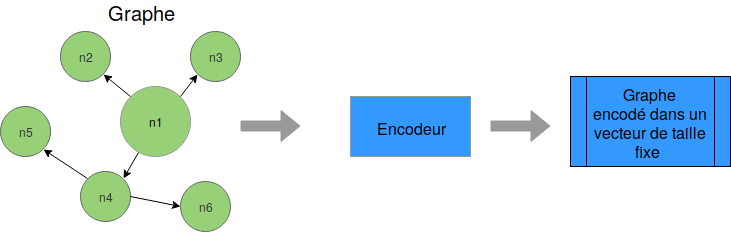
\includegraphics[width=0.9\linewidth]{images/Conception/DM/encoder.png}
	\caption{Schéma représentant un encodeur de graphe}
	
\end{figure}\label{encoder}
Ces méthodes nécessitent tout le graphe pour l'encoder. Cependant, dans notre cas, après chaque action, le graphe augmente de taille ce qui nécessite de refaire l'encodage à partir du début. Nous proposons de traiter le graphe comme une séquence de triplets: "n\oe{}ud; arc; n\oe{}ud" ou "sujet; predicat; objet" comme dans la représentation Resource Description Framework (RDF). L'encodage se fait avec une architecture encodeur-décodeur basée sur des réseaux de neurones récurrents (RNN). Ainsi, à l'arrivée de nouveaux triplets, il suffit d'utiliser l'état précédent pour pouvoir encoder les nouveaux triplets.
\begin{figure}[H] 
	\centering
	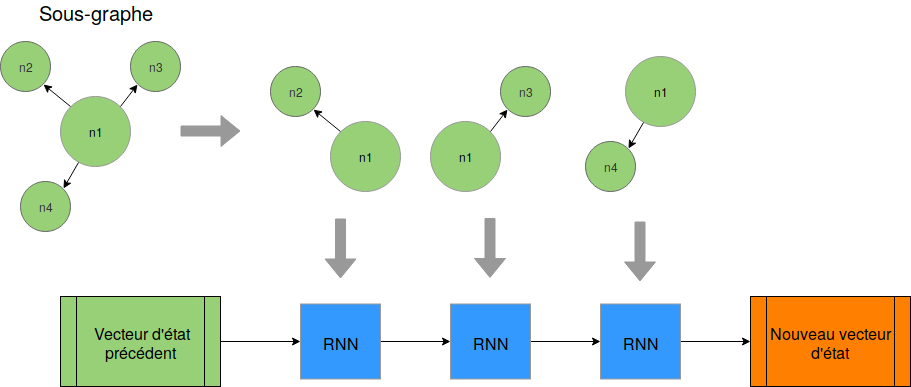
\includegraphics[width=0.8\linewidth]{images/Conception/DM/encoder_seq.png}
	\caption{Schéma représentant un encodeur séquentiel de graphe}
	
\end{figure}\label{encoder_seq}
Comme le montre la figure \ref{encoder_seq}, lorsque un sous-graphe arrive, celui-ci est décomposé en triplets. Ensuite, chaque triplet est encodé séquentiellement dans le vecteur d'état précédent qui encode déjà l'ancien état du graphe. Le résultat sera un vecteur d'état encodant la totalité du nouveau graphe.
\par Pour faire l'apprentissage de cette architecture, il est possible de générer des graphes aléatoirement qu'on fait passer triplet par triplet dans l'encodeur. Celui-ci est un RNN qui prend en entrée l'état précédent du réseau et un triplet du graphe et qui produit en sortie un nouvel état. L'état final du RNN, après avoir fait passer tous les triplets du graphe, est utilisé dans le décodeur qui est un autre RNN. Ce dernier essaye de reconstruire le graphe triplet par triplet à partir de l'état reçu comme sortie de l'encodeur. Ainsi, si on peut reconstruire le graphe, on peut dire que le dernier état encode tout le graphe dans un vecteur de taille fixe.
\begin{figure}[H] 
	\centering
	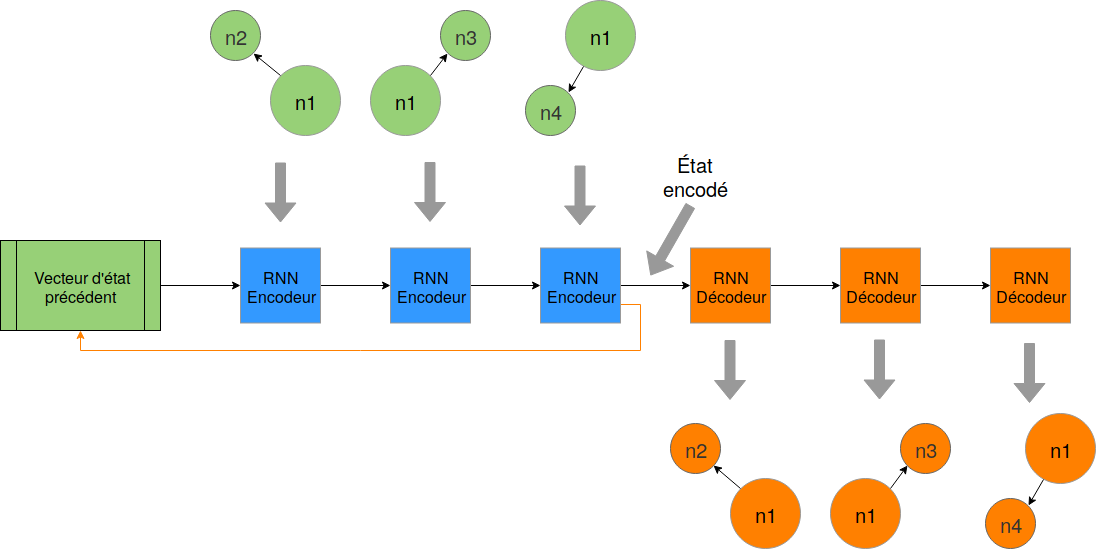
\includegraphics[width=0.9\linewidth]{images/Conception/DM/encoder_seq_train.png}
	\caption{Schéma de l'apprentissage d'un encodeur séquentiel de graphe}
	
\end{figure}\label{encoder_seq_train}
\subsubsection*{Les agents feuilles}
Comme nous l'avons cité précédemment, les agents feuilles sont les agents responsables de répondre aux intentions de l'utilisateur. Pour faire l'apprentissage par renforcement d'un agent feuille, nous utilisons le simulateur d'utilisateur comme environnement de cet agent. Ce dernier interagit avec le simulateur pour but d'estimer la correspondance des récompenses en fonction des états. Nous utilisons pour cela un réseau de neurones profond qui prend en entrée le graphe encodé de l'agent et produit pour chaque action la récompense correspondante. Comme le nombre d'actions est variable, il est impossible d'utiliser un réseau de neurones qui produit une récompense pour chaque action vu que les réseaux de neurones ont un nombre de sorties fixe. Par conséquent, il est nécessaire d'utiliser une architecture qui prend en entrée, en plus de l'état encodé, l'action candidate pour produire en sortie sa récompense.\newpage
\begin{figure}[H]
	\centering
	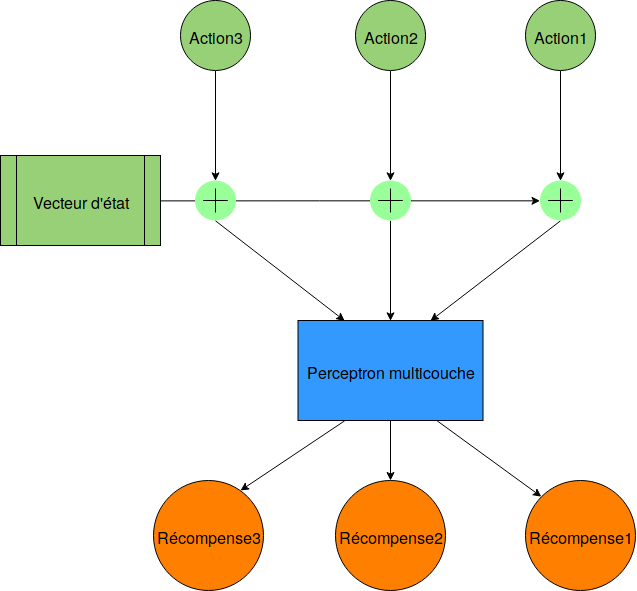
\includegraphics[width=0.5\linewidth]{images/Conception/DM/time_dist.png}
	\caption{Schéma du réseau DQN}
\end{figure}\label{time_dist}
L'algorithme utilisé pour l'apprentissage par renforcement est double DQN en rejouant l'expérience que nous détaillerons dans cette partie. En plus de l'utilisation des réseaux de neurones pour estimer la fonction Q, deux amélioration lui ont été ajoutées:
\begin{itemize}
	\item Rejouer l'expérience: l'agent interagit avec le simulateur plusieurs fois en gardant dans une mémoire ses interactions. Après chaque k épisodes\footnote{Un épisode est un ensemble d'interactions agent-simulateur jusqu'à l'aboutissement à un succès ou un échec} l'agent reprend la mémoire pour entraîner le réseau de neurones.
	\item Double DQN: la fonction Q est donnée par la formule $Q(s,a) = r + \alpha \times max_j(Q(s',a_j))$ \citep{Mnih2015} avec:
	\begin{itemize}
		\item $s$: état de l'agent.
		\item $a$: l'action qu'on veut estimer.
		\item $r$: récompense immédiate.
		\item $\alpha$: paramètre de réduction.
		\item $s'$: nouvel état après avoir effectué l'action $a$ de l'état $s$.
		\item $a_j$: les actions possibles à partir de l'état $s'$.
	\end{itemize}
	On remarque la récurrence dans cette formule qui nécessite la réutilisation du réseau pour estimer le terme $max_j (Q(s',a_j))$. Il a été démontré que l'utilisation d'un autre réseau qu'on fixe lors de l'apprentissage pour l'évaluation de la récompense dans ce terme améliore les résultats \citep{Mnih2015}. La formule devient donc: 
	\[Q(s,a) = r + \alpha \times Q(s',argmax_{a_j}(s',a_j))\]
	Cette valeur est donc utilisée comme cible du réseau DQN et permet de calculer l'erreur moyenne quadratique par rapport à sa prédiction. Ensuite l'algorithme de retro-propagation est appliqué pour l'apprentissage automatique.
\end{itemize}
Une autre architecture possible serait de relier l'encodeur de graphe directement avec le réseau DQN pendant l'apprentissage. Ainsi l'erreur de l'apprentissage pour l'encodeur est calculée à partir de la fonction de récompenses de l'apprentissage par renforcement. L'avantage de relier l'encodeur avec le réseau DQN est de permettre à l'encodeur de contrôler quelle partie du graphe encodé à oublier. En effet, la taille fixe du vecteur dont on encode le graphe a une limite de nombre de triplets supportable. L'utilisation des cellules de réseaux de neurones récurrents comme les LSTMs ou GRUs qui ont des portes d'oubli rend cette architecture possible. En effet, ce type de RNNs ont la possibilité de garder en mémoire (leur état) des informations qu'ils ont reçues au début de la séquence de données en sacrifiant d'autres plus récentes. en d'autres termes, ils peuvent choisir quelles sont les informations à garder dont le DQN aura besoin pour estimer la fonction de récompense.
\begin{figure}[H] 
	\centering
	\includegraphics[width=0.88\linewidth]{images/Conception/DM/encoder_dqn.png}
	\caption{Schéma du réseau DQN relié avec l'encodeur directement}
\end{figure}\label{encoder_dqn}
\subsubsection*{L'agent coordinateur}
L'agent coordinateur utilise la même architecture que celle des agents feuilles. La différence se trouve au niveau de la sortie. Dans le cas des agents coordinateurs, ils essayent de prédire quel agent fils peut répondre à la dernière action reçue.
\section{Module de génération du langage naturel}
Le modèle utilisé pour la génération du texte est relativement simple. Il s'agit de préparer des modèles de phrases contenant des emplacements à remplir. Chaque action de l'agent correspond à un ensemble de modèles et à chaque paramètre de l'action correspond un ensemble d'expressions. La génération du texte se fait en choisissant d'abord pour chaque paramètre de l'action une expression aléatoirement. Ensuite un modèle de phrase est choisi aléatoirement. Enfin, les emplacements vides sont remplis avec les expressions des paramètres. Le module de génération de texte traite aussi les éventuelles erreurs qui peuvent se produire comme la suppression d'un fichier inexistant ou la création d'un fichier qui existe déjà. Dans ce cas, l'agent doit informer l'utilisateur que l'action demandée ne peut pas être exécutée pour qu'il résolve le problème. Le traitement des erreurs est similaire au traitement des actions. Le générateur de texte utilise le nom de l'erreur comme l'intention de l'agent et ses paramètres comme les paramètres de l'action.
\begin{figure}[H] 
	\centering
	\includegraphics[width=0.95\linewidth]{images/Conception/NLG.png}
	\caption{Schéma de fonctionnement du générateur de texte}\label{nlg_schema}
\end{figure}
Dans la figure \ref{nlg_schema} un exemple de génération de texte en utilisant les modèles de phrases est présenté où l'agent demande à l'utilisateur de lui donner le répertoire parent d'un fichier nommé "travail". Le générateur de texte utilise l'intention de l'agent "$Request$" pour extraire les modèles de phrases qui lui correspondent. En parallèle, il utilise les paramètres de l'action pour extraire leurs expressions. Par exemple, le nom du fichier peut être transformé en "\textit{travail}" ou "\textit{the file travail}". Ces expressions sont enfin combinées avec le modèle de la phrase choisi pour générer une phrase complète. Par exemple, "\textit{Please, tell me what is the \textbf{parent directory}} of \textbf{travail}" ou "\textit{Please, tell me what is the \textbf{directory} of \textbf{the file travail}}".
\section{Conclusion}
\paragraph{}
Dans ce chapitre, et en nous inspirant des travaux existants, nous avons pu modéliser et conceptualiser tout les aspects du système que nous jugeons assez conforme au standard. Viennent s'ajouter les améliorations proposées pour enrichir le système de base retrouvé dans la littérature ainsi que pour faciliter l'extensibilité des fonctionnalités de bases avec un moindre effort d'intégration. Ceci est le résultat d'une conception modulaire et facilement maintenable. 
\par Dans le chapitre suivant nous allons passer à l'implémentation des différents modules, au développement d'une application dédiée et à une partie expérimentation pour tester les approches proposées. Nous discuterons leurs améliorations et les comparer avec des standards existants.


\newpage
\chapter{Réalisation et résultats}
\section{Introduction}
\paragraph{}Dans la partie conception, nous avons proposé certaines modifications à apporter sur des approches existantes ainsi que des méthodes que nous avons jugées intéressantes pour notre système. Nous allons, dans la suite de ce chapitre, montrer la faisabilité de ces méthodes ainsi que leurs avantages et leurs limites.
\paragraph{}Nous commençons par décrire l'environnement de travail. Nous détaillerons par la suite les aspects de l'implémentation des différents modules de notre application qui seront évalués et analysés. Pour clôturer avec une application d'un assistant personnel pour la manipulation de fichiers. 

\section{Environnement de développement}
Dans cette section nous allons présenter les différents outils (logiciels et matériels) qui ont été utilisé pour l'implémentation de BETHANO.
	\subsection{Machines utilisées}
	\paragraph{}
	Principalement, le développement se divise en deux parties : 
	\begin{itemize}
		\item Apprentissage : les données sont récoltées ou construites puis nettoyées et préparées. Les modèles sont développés, entraînés puis testés.
		\item Les modules sont implémentés puis connectés et intégrés dans l'application.
	\end{itemize}
	\par Pour ce faire nous avons utilisé des machines dont les spécificités sont mentionnés ci-dessous :
	%TODO insert figures with their caption here OR one diagram with specs
	\begin{figure}[H] 
		\centering
		\includegraphics[width=0.88\linewidth]{images/implementation/machines.png}
		\caption{Caractéristiques des machines}
		\label{fig:machines}
		
	\end{figure}
	\par
	En ce qui concerne la partie logicielle, une liste non exhaustive est présentée ci dessous, qui ne mentionne que les outils les plus utilisés et les plus exploités :
	\subsection{Langages de programmation}
%		\begin{figure}[H] 
%		\centering
%		\includegraphics[width=0.3\linewidth]{images/implementation/langs.png}
%		\caption{Langages de programmation utilisés}
%		\label{fig:langs}
%	\end{figure}
		\subsubsection*{Python}
		\label{python}
		\paragraph{}
		 C'est un langage de programmation interprété de haut niveau, structuré et open source. Il est multi-paradigme (orienté objet, programmation fonctionnelle et impérative) et multi-usage. Il est, comme la plupart des applications et outils open source, maintenu par une équipe de développeurs un peu partout dans le monde. Il offre une grande panoplie d'extensions (packages) pour résoudre une variété de problèmes, qu'ils soient reliés au développement d'applications de bureau, web ou mobiles \cite{python}.
		
		\subsubsection*{Javascript} 
		\paragraph{}
		JavaScript est un langage de programmation utilisé principalement par les navigateurs web pour exécuter un bout de code incorporé dans une page web, plus communément appelé script. Il permet la manipulation de tous les éléments inclus dans une page, et par conséquent permet une gestion dynamique de ces derniers. Il est beaucoup utilisé du coté client mais peut aussi être exécuté du coté serveur. Tout comme Python, il offre une grande variété dans le choix des modules qui peuvent ajouter de nouvelles fonctionnalités, le tout géré par un gestionnaire de module \textit{npm} \footnote{Node Package Manager ou Gestionnaire de packages Node} devenu un standard \cite{js}.
	
	\subsection{Librairies et bibliothèques}
	\begin{figure}[H] 
		\centering
		\includegraphics[width=0.9\linewidth]{images/implementation/libs_frams.png}
		\caption{Bibliothèques et librairies les plus utilisées dans ce projet.}
		\label{fig:libs_frams}
	\end{figure}
		\subsubsection*{DeepSpeech API}
		\paragraph{}
		Package python qui fait office d'interface entre un script Python et la librairie de reconnaissance automatique de la parole DeepSpeech \cite{deepspeech_paper}. Il permet entre autres de charger différents modèles acoustiques ou modèles de langues. Il offre aussi la possibilité d'utiliser des scripts d'apprentissage prédéfinis pour peu que les données soient organisées suivant une certaine norme; ces scripts sont notamment hautement paramétrables \cite{deepseech_github}.
		
		\subsubsection*{PyAudio}
		\paragraph{}
		Librairie python destinée à la manipulation des fichiers ou flux audios. Elle offre entre autres la possibilité d'extraire des méta-données sur un flux audio (fréquence d'échantillonnage, débit ...). La possibilité d'extraire le vecteur de caractéristiques d'un extrait audio est aussi présente comme fonctionnalité \cite{pyaudio}.
		
		\subsubsection*{Beautiful Soup}
		\paragraph{}
		Bibliothèque Open source permettant l'analyse de fichiers html pour en extraire ou y injecter des données. Principalement utilisée pour filtrer les balises html depuis une page web \cite{bs4}.
		
		\subsubsection*{PySpark}
		\paragraph{}
		Package Python utilisé comme interface pour intéragir avec un serveur Spark. Il permet entre autres de lire et écrire des données dans le nouveau format Hadoop \cite{pyspark}.
		
		\subsubsection*{Scikit-Learn}
		\paragraph{}
		Bibliothèque Open source conçue pour rapidement développer des modèles pour l'apprentissage automatique, principalement utilisée pour ses nombreux outils de pré-traitement des données (codification, normalisation, filtrage ...) \cite{sklearn}.
		
		\subsubsection*{Numpy}
		\paragraph{}
		Bibliothèque spécialisée dans la manipulation de grands volumes de données numériques, notamment les vecteurs (tableaux) multi-dimensionnels. Les opérations sur ces derniers sont implémentées en C pour optimiser au maximum leur coût en temps de calcul ou ressources mémoires utilisées. Elle offre des structures de données compatibles avec beaucoup d'autre librairies comme Tensorflow ou Keras \cite{numpy}.
		
		\subsubsection*{Tensorflow \& Keras}\label{tf&keras}
		\paragraph{}
		Tensorflow est une bibliothèque dédiée à l'apprentissage automatique, et plus particulièrement aux réseaux de neurones et l'apprentissage profond. Optimisée pour exécuter des opérations à grande échelle et massivement distribuées sur un réseau, Tensorflow offre la possibilité d'implémenter une grande variété d'architectures de modèles avec un maximum d'efficacité. Elle dispose d'un package Python permettant d'interagir avec le c\oe{}ur de la bibliothèque mais reste néanmoins assez bas-niveau. Keras quant-à elle propose de rajouter une couche d'abstraction à Tensorflow. C'est un package python destiné à faciliter le développement de modèles pour l'apprentissage profond tout en offrant la possibilité de rajouter et modifier un grand nombre de fonctionnalités par défaut. Sa force réside dans le fait qu'il peut utiliser au plus bas niveau plusieurs librairies autres que Tensorflow comme Theano et CNLTK \cite{tf,keras,theano,cnltk}.
		
		\subsubsection*{Flask}
		\paragraph{}
		Micro-librairie Open source dédiée au développement d'applications basées web. De base, cette librairie est très légère, mais elle offre la possibilité d'ajouter des extensions qui s'intègrent très facilement au système de base \cite{flask}.
		
		\subsubsection*{Vuetify}
		\paragraph{}
		Librairie Open source basée sur VueJs dédié au développement d'interfaces web ou mobiles. Elle implémente le paradigme Material Design de Google et offre la possibilité d'étendre les composants de base et de créer des interfaces belles et adaptatives \cite{vuetify}.
	\subsection{Outils et logiciels de développement}
		\subsubsection*{PyCharm}
		\paragraph{}
		PyCharm est un environnement de développement intégré spécialisé et optimisé pour programmer dans le langage Python (voir \ref{python} ci dessus). Il permet l'analyse de code en continu et offre un débogueur intégré pour exécuter un code instruction par instruction. Il offre également l'intégration de logiciel de gestion de versions comme Git \cite{git}, et supporte le développement web avec Django et Flask \cite{pycharm}.
		
		\subsubsection*{Git}
		\paragraph{}
		Système décentralisé de gestion de versions. Il permet entre autres de gérer les différentes versions d'un projet durant son développement, mais aussi de garder l'historique des modifications effectuées ainsi que la possibilité de régler des conflits lors de l'intégration finale des contributions des développeurs \cite{Git}.
		
		\subsubsection*{Google Colaboratory}
		\paragraph{}
		Colaboratory est un outil de recherche et développement pour la formation et la recherche associées à l'apprentissage profond. C'est un environnement Python qui ne nécessite aucune configuration et offre la possibilité d'utiliser de puissantes machines rendues accessibles par Google pour accélérer la phase d'apprentissage \cite{colab}.
		
		\subsubsection*{Protégé}
		\paragraph{}
		Protégé est un système dédié à la création et la modification d'ontologies. Il est développé en Java et est Open source distribué sous une licence libre (la Mozilla Public License). Il se démarque par le fait qu'il permet de travailler sur des ontologies de très grandes dimensions 
		\cite{protege}.
		
		
\section{Reconnaissance automatique de la parole}
\paragraph{}
Pour ce premier module, il a été très difficile d'effectuer les tests idéaux. En effet, nous n'avons pas pu trouver un ensemble de données qui proposait du contenu en rapport avec Bethano. Cependant puisque nous avons pu construire un mini-ensemble pour tester l'apport de notre modèle de langue. Les résultats ne doivent pas être pris comme une référence absolue, mais plutôt comme une indication pour de futurs possibles tests.
	\subsection{Ensemble de test}
	\paragraph{}
	Pour tester le modèle acoustique, les données récoltées à travers le projet CommonVoice \ref{common_voice} constituent un assez bon échantillon, de par la nature des enregistrements (sur téléphone portable, par plusieurs genres et accents de locuteurs ...), mais aussi de par le volume (environs 500 heures d'enregistrements audios). Nous avons toutefois décidé de construire un mini-ensemble de test d'environs 204 enregistrements audio d'une longueur moyenne de 5 secondes chacun. Ces échantillons ont été prélevés sur trois locuteurs masculins. $20\%$ de ces échantillons ont été prélevés dans un environnement fermé mais bruité (il s'agit d'un espace de travail pour étudiants) et sur téléphone. Le reste a été prélevé dans un environnement fermé avec peu de bruit à partir du micro d'un ordinateur portable. Chaque enregistrement est soit : 
	\begin{itemize}
		\item une requête prélevée de l'ensemble de test du module de compréhension du langage naturel (voir les sections \ref{nlu_steps} et ~\ref{nlu_dataset}), ou
		
		\item une question prélevée de l'ensemble de données AskUbuntu\footnote{\url{https://github.com/taolei87/askubuntu}} qui regroupe des questions relatives à la manipulation d'un ordinateur sous le système d'exploitation GNU/Linux.
	\end{itemize}
	\par
	Pour le modèle de langue il s'agit de celui mentionné dans la section \ref{LM_n-grams}. Quelques modifications ont été rajoutées comme le filtrage des mots qui n'appartiennent pas à la langue anglaise, mais au prix du sacrifice de quelques noms propres non reconnus ou bien de séquences de mots/lettres sans réel sens.
	\subsection{Méthodologie d'évaluation}
	\paragraph{}
	Les tests ont été effectués dans un serveur Colab pour libérer les machines locales. Les principales étapes sont les suivantes :  
	\begin{enumerate}
		\item \textbf{Préparation des données} : Les données sont prélevées d'une base de données sqlite qui comprend une seule table Transcriptions. Les colonnes de la table sont : 
		\begin{itemize}
			\item \textbf{id} : identifiant de l'enregistrement
			\item \textbf{path} : chemin vers le fichier audio de la requête.
			\item \textbf{text} : transcription textuelle de la requête.
		\end{itemize}
		\par
		Un script de conversion est ensuite lancé pour s'assurer que chaque enregistrement est au format .wav avec une fréquence de rafraîchissement égale à 16KHz (le modèle acoustique de DeepSpeech attend cette valeur exacte pour lancer l'inférence, sinon une erreur se produira).
		
		\item \textbf{Métriques retenues} : À chaque instance testée, le \textbf{WER} (Word Error Rate) est calculé. Pour rappel la formule du WER est la suivante :
		\begin{equation*}
			WER(y,\hat{y}) = \frac{S+D+I}{S+D+C} = \frac{S+D+I}{N}
		\end{equation*}
		où : 
		\begin{itemize}
			\item $\hat{y}$ est la séquence de mots prédite appelée Hypothèse.
			\item $y$ est la séquence de mots réelle appelée Référence.
			\item $S$ est le nombre de substituions (compté en mots) réalisées entre l'hypothèse et la référence.
			\item $D$ est le nombre de suppressions qu'a effectué le système, donc le nombre de mots supprimés dans l'hypothèse par rapport à la référence.
			\item $I$ est le nombre d'insertions effectuées par le système (c.à.d, le nombre de mots rajoutés à l'hypothèse par rapport à la référence).
			\item $C$ est le nombre de mots bien placés.
			\item $N$ est la longueur totale de la séquence en nombre de mots
		\end{itemize}
		\item \textbf{Boucle d'évaluation} l'opération précédente est réitérée en incrémentant à chaque fois le taux d'utilisation de notre modèle de langue (de 20\% à 100\% avec un pas de 10\%). Le WER associé est ensuite comparé à celui obtenu en utilisant le modèle de langue par défaut que propose DeepSpeech, le modèle acoustique sans modèle de langue, le résultat de l'API de Google \footnote{\url{https://cloud.google.com/speech-to-text/}} et enfin le modèle par défaut de CMU Sphinx \footnote{\url{https://cmusphinx.github.io/}}
		
	\end{enumerate}
	\subsection{Résultats}
	\paragraph{}
	Les résultats sont décrits dans le tableau \ref{tab:asr_results} et la figure \ref{fig:asr_results}. Nous remarquons que sur notre mini-ensemble de test, les modèles par défaut obtiennent un score très proche de 1, ce qui démontre qu'ils ont été entraînés sur des cas assez généraux, ce qui n'est pas très bon. Cependant, en changeant juste le modèle de langue par défaut en injectant des échantillons, une nette amélioration est visible (environ $-20\%$). Ce taux d'erreur diminue en augmentant la taille du corpus utilisé pour le modèle de langue. Toutefois, après avoir pris plus de $75\%$ du corpus, l'erreur a légèrement augmenté. Cela peut s'expliquer par la nature assez bruitée du corpus, les fichiers README.MD qui sont rédigés par des personnes, l'erreur humaine, et l'absence de processus de vérification de l'orthographe, de la grammaire ou de la syntaxe du contenu. Nous avions envisagé de choisir comme corpus des extraits de livres dédiés à la manipulation des ordinateurs sous Linux, mais nous n'avons pas trouvé de ressources gratuites ou Open source exploitables.
	\par
	Il est à noter que le meilleur résultat obtenu, c.à.d un taux d'erreur de $72.6\%$ est très loin d'être satisfaisant comparé au taux d'erreur de l'API de Google par exemple qui est d'approximativement $0.3496\%$. Néanmoins, l'ajout d'un modèle de langue personnalisé a pu améliorer nettement les résultats observés durant l'utilisation du modèle de base. Comme mentionné dans la section \ref{asr_probs}, DeepSpeech reste la meilleure option en Open Source à notre portée.
	\begin{table}[H]
		\centering
		\resizebox{\textwidth}{!}{%
			\begin{tabular}{c|c|}
				\cline{2-2}
				& WER (Word Error Rate) \\ \hline
				\multicolumn{1}{|c|}{Goole API} & 0,34955014 \\ \hline
				\multicolumn{1}{|c|}{Modèle acoustique avec 50\% du corpus} & 0,72634931 \\ \hline
				\multicolumn{1}{|c|}{Modèle acoustique avec 75\% du corpus} & 0,72809889 \\ \hline
				\multicolumn{1}{|c|}{Modèle acoustique avec 100\% du corpus} & 0,72928369 \\ \hline
				\multicolumn{1}{|c|}{Modèle acoustique avec 25\% du corpus} & 0,73910913 \\ \hline
				\multicolumn{1}{|c|}{Modèle acoustique - 10\% du corpus} & 0,74333040 \\ \hline
				\multicolumn{1}{|c|}{Modèle acoustique et modèle de langue de base} & 0,79569078 \\ \hline
				\multicolumn{1}{|c|}{Modèle acoustique seulement} & 0,91092787 \\ \hline
				\multicolumn{1}{|c|}{CMU Sphinx de base} & 0,94024028 \\ \hline
			\end{tabular}%
		}
		\caption{Tableau récapitulatif des résultats pour le module de reconnaissance automatique de la parole.}
		\label{tab:asr_results}
	\end{table}
	\begin{figure}[H]
		\centering
		\includegraphics[width=.9\linewidth]{images/implementation/asr_graph.png} 
		\caption{Graphe récapitulatif des résultats pour le a reconnaissance automatique de la parole}
		\label{fig:asr_results}
	\end{figure}
\section{Classification d'intentions et extractions d'entités de domaine}
\paragraph{}
Pour ce module, une approche assez classique a été utilisée et l'ensemble de test est extrait de l'ensemble d'apprentissage (plus de détails dans la section suivante ). Les métriques d'évaluation utilisées sont mentionnées dans la sous section \ref{nlu_steps}. Nous commençons d'abord par détailler le contenu de l'ensemble de tests. Puis nous présenterons la méthodologie suivie pour la réalisation de ces tests. Un tableau récapitulatif sera présenté avant la fin pour illustrer les différents résultats.
	\subsection{Ensemble de test}
	\paragraph{}
	Comme mentionné dans le chapitre précédent (voir la section \ref{nlu_dataset}), nous avons nous mêmes construit un ensemble d'apprentissage relativement varié. Il regroupe essentiellement des commandes, ou requêtes liées à l'exploration de fichiers pour le moment car c'est la tâche rudimentaire que Bethano peut accomplir.
	\par
	L'ensemble de test est dérivé de celui d'apprentissage selon une politique de découpage basée sur le taux de présence d'un intent (intention). Comme illustré dans la figure \ref{fig:split}, un pourcentage de chaque groupe d'instances affilié à la même classe est utilisé à la fois pour la validation et pour le test. Ce choix est motivé par le fait que les proportions des distributions des intentions dans l'ensemble original sont non-équilibrées.
	
	Une liste exhaustive des intentions et slots accompagnée d'une description est introduite dans le tableau \ref{tab:all_intents} ci dessous.
%	TODO insert table of intents and their tags
%	TODO figure here for ratio splitting  
	\begin{figure}[H]
		\centering
		\includegraphics[width=.75\linewidth]{images/implementation/split.png} 
		\caption{Schéma de découpage des données pour l'apprentissage du modèle de compréhension du langage naturel} 
		\label{split}
	\end{figure}

	\begin{table}[H]
		\centering
		\resizebox{\textwidth}{!}{%
			\begin{tabular}{|c|c|c|l|}
				\hline
				\textbf{Intention} & \textbf{\begin{tabular}[c]{@{}c@{}}Description \\ de l'intention\end{tabular}} & \textbf{Groupe} & \multicolumn{1}{c|}{\textbf{\begin{tabular}[c]{@{}c@{}}Argument(s)\\ ( Entité(s) )\end{tabular}}} \\ \hline
				create\_file\_desire & Création d'un fichier & ALTER & \begin{tabular}[c]{@{}l@{}}-file\_name\\ -parent\_directory\end{tabular} \\ \hline
				create\_directory\_desire & Création d'un répertoire & ALTER & \begin{tabular}[c]{@{}l@{}}-directory\_name\\ -parent\_directory\end{tabular} \\ \hline
				delete\_file\_desire & Suppression d'un fichier & ALTER & \begin{tabular}[c]{@{}l@{}}-file\_name\\ -parent\_directory\end{tabular} \\ \hline
				delete\_directory\_desire & Suppression d'un répertoire & ALTER & \begin{tabular}[c]{@{}l@{}}-directory\_name\\ -parent\_directory\end{tabular} \\ \hline
				open\_file\_desire & Ouverture d'un fichier & INFO & \begin{tabular}[c]{@{}l@{}}-file\_name\\ -parent\_directory\end{tabular} \\ \hline
				close\_file\_desire & Fermeture d'un fichier & INFO & \begin{tabular}[c]{@{}l@{}}-file\_name\\ -parent\_directory\end{tabular} \\ \hline
				copy\_file\_desire & Copie d'un fichier & ALTER & \begin{tabular}[c]{@{}l@{}}-file\_name\\ -origin\\ -destination\end{tabular} \\ \hline
				move\_file\_desire & Déplacement d'un fichier & ALTER & \begin{tabular}[c]{@{}l@{}}-file\_name\\ -origin\\ -destination\end{tabular} \\ \hline
				rename\_file\_desire & Renommage d'un fichier & - & \begin{tabular}[c]{@{}l@{}}-old\_name\\ -new\_name\end{tabular} \\ \hline
				change\_directory\_desire & \begin{tabular}[c]{@{}c@{}}Changement du répertoire \\ de travail courant\end{tabular} & - & -new\_directory \\ \hline
				inform & Informer d'une intention & EXCH & \begin{tabular}[c]{@{}l@{}}-file\_name\\ -parent\_directory\end{tabular} \\ \hline
				request & Demander une information & EXCH & \begin{tabular}[c]{@{}l@{}}-file\_name\\ -directory\end{tabular} \\ \hline
				deny & Réponse négative & - & \multicolumn{1}{c|}{-} \\ \hline
				confirm & Réponse positive & - & \multicolumn{1}{c|}{-} \\ \hline
				unknown & Intention inconnue & - & \multicolumn{1}{c|}{-} \\ \hline
			\end{tabular}%
		}
		\caption{Tableau récapitulatif de toutes les intentions avec leurs descriptions et leurs arguments.}
		\label{tab:all_intents}
	\end{table}
	\paragraph{}
	Les intentions sont regroupées en groupes; chaque groupe comporte des intentions qui influent sur les documents de la même manière. Il existe bien évidemment des intentions sans groupe (on peut considérer qu'ils forment un seul groupe, ou bien que chacun constitue son propre groupe) : 
	\begin{itemize}
		\item \textbf{ALTER} : Groupe d'intentions qui altère l'état d'un document.
		\item \textbf{INFO} : Groupe d'intentions pour effectuer une opération puis informer l'utilisateur.
		\item \textbf{EXCH} : Groupe d'intentions dont le but est d'échanger des informations avec l'utilisateur.
	\end{itemize}
	\subsection{Méthodologie d'évaluation}
	\label{nlu_steps}
	\paragraph{}
	Après avoir construit l'ensemble de test, un parcours exhaustif des différentes combinaisons des paramètres suivants est effectué : 
	\begin{itemize}
		\item \textbf{Architecture d'encodage} :
		C'est à dire l'utilisation ou pas d'un réseau récurrent LSTM de base ou bien BiLSTM. Le but étant de montrer que le modèle pourra mieux interpréter les données en entrée s'il capture le contexte de chaque mot.
		
		\item \textbf{Nombre neurones pour la couche de classification d'intention } : Lorsque l'encodeur retourne le dernier vecteur d'état caché, ce dernier passera par un réseau de neurones complètement connecté et multi-couches (nombre de couches fixé à 3 par souci de performance, une couche d'entrée, une couche intermédiaire et une couche de sortie). Le nombre de neurones sur la couche cachée dépend grandement de la complexité de la tâche à effectuer. La classification d'intentions pour l'exploration de fichier était relativement simple; nous avons commencé avec 32 neurones puis nous avons doublé ce nombre jusqu'à 512 pour, en théorie, donner plus de puissance au classificateur tout en évitant un sur-apprentissage par surplus de neurones.
		
		\item \textbf{Nombre d'unités d'une cellule LSTM (respectivement BiLSTM)}:
		En effet, les portes d'une cellule LSTM (resp. BiLSTM) sont en vérité des réseaux de neurones denses (complètement connectés) et donc un ensemble de matrices de poids à optimiser. La capacité à "apprendre" la représentation des séquences dépend donc aussi du nombre de neurones dans ces mini-réseaux. Par le même raisonnement employé pour le classificateur d'intentions, nous avons commencé avec un petit nombre de neurones pour examiner où se trouverait le seuil minimal qui permettra au modèle de généraliser, mais aussi où le seuil critique se situerait pour permettre au modèle de ne pas tomber dans un cas de sur-apprentissage. Nous partons de 128 jusqu'à 512 unités avec pas de 32 unités.
		
		\item \textbf{Fonctions d'activations} : 
		C'est un élément essentiel qui permet d'introduire la non-linéarité dans les relations entre chaque neurones de couches voisines. Ces fonctions permettent de mieux représenter les seuils d'activations des neurones. La fonction la plus utilisée dans la littérature est actuellement ReLu (Rectified Linear Unit) car elle a expérimentalement donné de meilleurs résultats dans une grande variété de tâches et problèmes liés à l'apprentissage automatique et à la classification et étiquetage de textes. Par souci d'exhaustivité nous avons quand même décidé de tester deux autres fonctions $tanh$ (Tangente Hyperbolique) et $sigmoid$ (Sigmoïde). Pour chaque couche de sortie, la fonction $Softmax$ à été appliquée car chaque couche traite d'un problème de classification multi-classes. Voici les équations pour chacune de ces fonctions :
%		TODO equations for fucntions
		\begin{equation*}
			\tanh{x} = \frac{e^{x}-e^{-x}}{e^x+e^{-x}}
		\end{equation*}
		
		\begin{equation*}
			sigmoid(x) = \frac{1}{1+e^{-x}}
		\end{equation*}
		
		\begin{equation*}
			softmax_i(x) = \frac{e^{x_i}}{\sum_{j=1}^{K}e{^x_j}} \text{ pour } i=1,...,K \text{ et } x=(x_1,...,x_K) \in \mathbb{R}^K
		\end{equation*}
		\item \textbf{Fonction erreur}:
		C'est l'élément clé pour la phase d'apprentissage, cette fonction détermine le degré d'exactitude du modèle, c'est à dire à quel point il est proche de la bonne réponse. Nous avons décidé d'utiliser comme fonction erreur la fonction $Categorical\_Crossentropy$ ou Erreur Logistique; de par la nature de l'ensemble d'apprentissage et de test. Une version pondérée de cette fonction a été préférée, pour palier au problème du non équilibrage des classes, que ce soit pour la classification d'intentions, ou pour la reconnaissance d'entités du domaine.\\
		\par
		Les poids des classes sont calculés selon la formule suivante : 
		
		\begin{equation*}
			Poids_i = \max(1,\log{\frac{T}{T_i}})
		\end{equation*}
		où :
		\begin{itemize}
			\item  $T$ est le nombre total d'instances
			\item  $T_i$ est le nombre d'instances dont la classe est $C_i$
		\end{itemize}
		
		La formule de la fonction erreur devient donc : 
		\begin{equation*}
			Erreur(y,\hat{y}) = - \sum_{i}^{C} y_i * \log(\hat{y}_i) * Poids_i 
		\end{equation*}
		où : 
		\begin{itemize}
			\item $\hat{y}$ est le vecteur en sortie produit par le modèle à la suite d'une fonction $Softmax$.
			\item $y$ est le vecteur de classe réelle présent dans l'ensemble d'apprentissage
			\item $C$ est le nombre de classes au total.
		\end{itemize}
	
		\item \textbf{Fonction d'apprentissage}:
		Le choix de la fonction d'apprentissage est généralement affecté par un désir de précision et de rapidité. Une fonction qui converge rapidement en un minimum local peut être parfois préférée à une autre qui prendrait un temps considérable pour soit se retrouver dans le même minimum ou un autre minimum local (donc sans garantie de minimum optimal de la fonction erreur). Les deux fonctions utilisées sont RmsProp et Adam qui sont connues pour leur rapidité de convergence.
		
		\item \textbf{Encodage des entrée-sorties}:
		Là encore le choix de l'encodage des données influe grandement sur la capacité du modèle à distinguer et à représenter les différentes informations qui lui sont présentées. Comme initiative de notre part, nous avons mentionné dans la section \ref{nlu_dataset} l'ajout de l'étiquette morphosyntaxique de chaque mot à l'encodage. Nous avons donc lancé les tests sur un encodage avec (respectivement sans) l'ajout des étiquettes pour mieux constater son impact.
		
		\item \textbf{Découpage des données}
		La stratégie adoptée était de prendre aléatoirement les même proportions pour chaque sous-ensemble de chaque classe (intentions ou entités de domaine). Nous avons aussi décidé de faire varier les proportions de test et d'apprentissage en fixant celui de validation car nous avons remarqué que notre modèle n'arrivait pas à bien généraliser la relation entre les entrées et les sorties. Notre intuition portait sur le fait que le manque de données pouvait en être la cause (voir la section \ref{nlu_dataset} pour plus de détails). Ainsi, nous avons varié le taux de découpage pour les données de tests entre $25\%$ et $75\%$ avec un pas de $25\%$. Le taux de découpage pour l'apprentissage est évidement de $(100\%-T_{test})*90\%$.
		\par
		Pour éviter que le modèle ne sur-apprenne, nous avons volontairement interchangé quelques mots dans la séquence d'entrée et celle de sortie pour introduire un certain taux d'erreur et de variété. Cet échange se fait suivant une probabilité $q$ fixée à $20\%$. Bien entendu, les étiquettes morphosyntaxiques ne sont pas échangées, et ce pour garder la structure de la phrase correcte.
	\end{itemize}
	\par
	Pour le reste des hyper-paramètres, la plupart ont été fixés par manque de temps et de ressources. Ainsi, le nombre d'epochs (itérations) a été limité au maximum à 15 avec une politique d'arrêt anticipé si la fonction erreur d'évaluation ne diminue pas plus d'un taux $\Delta E = 2*10^{-3}$ pendant au moins 3 itérations successives. Les métriques employées pour évaluer les deux classificateurs sont les suivantes : 
	\begin{itemize}
		\item \textbf{Précision} : il s'agit d'une métrique classique qui évalue à quel point le modèle est bon pour prédire les classes.
		\begin{equation*}
			P = \frac{VP}{VP+FP}
		\end{equation*}
		où : 
		\begin{itemize}
			\item $VP$ (Vrais Positifs) : nombre de cas où le modèle prédit correctement la classe comme étant positive.
			\item $FP$ (Faux Positifs) : nombre de cas où le modèle ne prédit pas correctement la classe comme étant positive.
		\end{itemize}

		\item \textbf{Rappel} : Cette métrique évalue la capacité du modèle à effectuer des classifications correctes par rapport à tout l'ensemble de test. Plus formellement : 
		\begin{equation*}
		R = \frac{VP}{VP+FN}
		\end{equation*}
		où : 
		\begin{itemize}
			\item $FN$ (Faux Négatifs) : nombre de cas où le modèle ne prédit pas correctement la classe comme étant négative.
		\end{itemize}
	
		\item \textbf{F-Mesure} : Mesure qui combine (d'une point de vu ensembliste) la précision et le rappel. Elle ne privilégie aucune des deux et essaye de donner un aperçu plus global de l'efficacité de l'algorithme en prenant compte des résultats de ces deux mesures.
		\begin{equation*}
		F-mesure = \frac{2*R*P}{R+P}
		\end{equation*}
	\end{itemize}
	\subsection{Résultats}
	\paragraph{}
	Pour les résultats qui vont suivre, chaque tableau sera accompagné d'un paragraphe qui servira de commentaire aux résultats obtenus. Des remarques peuvent y être insérées pour attirer l'attention sur des détails non évidents.
	
	% Please add the following required packages to your document preamble:
	% \usepackage{graphicx}
	\begin{table}[H]
		\centering
		\resizebox{\textwidth}{!}{%
			\begin{tabular}{|c|c|c|c|c|c|c|c|c|}
				\hline
				\textbf{\begin{tabular}[c]{@{}c@{}}Nombre de\\ neurones\end{tabular}} & \textbf{\begin{tabular}[c]{@{}c@{}}Unités\\ LSTM\end{tabular}} & \textbf{Activation} & \textbf{Apprentissage} & \textbf{\begin{tabular}[c]{@{}c@{}}Précision\\ Intention\end{tabular}} & \textbf{\begin{tabular}[c]{@{}c@{}}Rappel\\ Intention\end{tabular}} & \textbf{\begin{tabular}[c]{@{}c@{}}Précision\\ Entités de\\ domaine\end{tabular}} & \textbf{\begin{tabular}[c]{@{}c@{}}Rappel\\ Entités de\\ domaine\end{tabular}} & \textbf{\begin{tabular}[c]{@{}c@{}}F-Mesure\\ moyenne\end{tabular}} \\ \hline
				32 & 128 & relu & rmsprop & 0,9743 & 0,9725 & 0,9214 & 0,9128 & 0,9452 \\ \hline
				32 & 256 & relu & rmsprop & 0,9755 & 0,9741 & 0,9066 & 0,8985 & 0,9387 \\ \hline
				32 & 512 & relu & rmsprop & 0,9750 & 0,9735 & 0,9082 & 0,9019 & 0,9396 \\ \hline
				64 & 128 & relu & rmsprop & 0,9700 & 0,9689 & 0,8744 & 0,8636 & 0,9192 \\ \hline
				64 & 256 & relu & rmsprop & 0,9753 & \textbf{0,9743} & 0,9141 & 0,9061 & 0,9424 \\ \hline
				\rowcolor[HTML]{96FFFB} 
				64 & 512 & relu & rmsprop & 0,9687 & 0,9669 & \textbf{0,9293} & 0,9230 & \textbf{0,9470} \\ \hline
				128 & 128 & relu & rmsprop & 0,9638 & 0,9626 & 0,8425 & 0,8283 & 0,8993 \\ \hline
				128 & 256 & relu & rmsprop & 0,9714 & 0,9707 & 0,8431 & 0,8345 & 0,9049 \\ \hline
				128 & 512 & relu & rmsprop & 0,9647 & 0,9635 & 0,8690 & 0,8584 & 0,9139 \\ \hline
				256 & 128 & relu & rmsprop & 0,9704 & 0,9692 & 0,8473 & 0,8342 & 0,9052 \\ \hline
				256 & 256 & relu & rmsprop & 0,7215 & 0,7141 & 0,7573 & 0,7275 & 0,7299 \\ \hline
				256 & 512 & relu & rmsprop & 0,9716 & 0,9711 & 0,8842 & 0,8761 & 0,9257 \\ \hline
			\end{tabular}%
		}
		\caption{Résultats des tests pour un encodage sans étiquetage morphosyntaxique avec des cellules LSTM avec découpage Apprentissage : 25\%, Validation : 10\%, Test : 75\%.}
		\label{tab:lstm_1}
	\end{table}
	
	\paragraph{}
	Nous pouvons remarquer depuis le tableau \ref{tab:lstm_1} que pour un ensemble d'apprentissage assez réduit, le modèle arrive tout de même à bien classifier la majorité des intentions avec un rappel maximum de $97,43\%$. Cependant le slot-filling se révèle être une tâche plus ardue avec un rappel ne dépassant pas $92,30\%$. La meilleure combinaison qui équilibre les deux tâches utilise un petit nombre de neurones pour la classification d'intentions, mais en revanche demande une grande capacité de calcul pour la mémorisation des séquences en utilisant 512 unités dans les cellules LSTM.
	
	% Please add the following required packages to your document preamble:
	% \usepackage{graphicx}
	\begin{table}[H]
		\centering
		\resizebox{\textwidth}{!}{%
			\begin{tabular}{|c|c|c|c|c|c|c|c|c|}
				\hline
				\textbf{\begin{tabular}[c]{@{}c@{}}Nombre de\\ neurones\end{tabular}} & \textbf{\begin{tabular}[c]{@{}c@{}}Unités\\ LSTM\end{tabular}} & \textbf{Activation} & \textbf{Apprentissage} & \textbf{\begin{tabular}[c]{@{}c@{}}Précision\\ Intention\end{tabular}} & \textbf{\begin{tabular}[c]{@{}c@{}}Rappel\\ Intention\end{tabular}} & \textbf{\begin{tabular}[c]{@{}c@{}}Précision\\ Entités de\\ domaine\end{tabular}} & \textbf{\begin{tabular}[c]{@{}c@{}}Rappel\\ Entités de\\ domaine\end{tabular}} & \textbf{\begin{tabular}[c]{@{}c@{}}F-Mesure\\ moyenne\end{tabular}} \\ \hline
				32 & 128 & relu & rmsprop & 0,9736 & 0,9721 & 0,8894 & 0,8817 & 0,9292 \\ \hline
				32 & 256 & relu & rmsprop & 0,9746 & 0,9735 & 0,9344 & 0,9298 & 0,9531 \\ \hline
				32 & 512 & relu & rmsprop & 0,9721 & 0,9714 & 0,9149 & 0,9089 & 0,9418 \\ \hline
				64 & 128 & relu & rmsprop & 0,9687 & 0,9684 & 0,9344 & 0,9286 & 0,9500 \\ \hline
				64 & 256 & relu & rmsprop & 0,9737 & 0,9729 & 0,9389 & 0,9325 & 0,9545 \\ \hline
				64 & 512 & relu & rmsprop & 0,9741 & 0,9732 & 0,9257 & 0,9188 & 0,9479 \\ \hline
				\rowcolor[HTML]{96FFFB} 
				128 & 128 & relu & rmsprop & 0,9684 & 0,9674 & 0,9354 & 0,9299 & \textbf{0,9503} \\ \hline
				128 & 256 & relu & rmsprop & 0,9709 & 0,9703 & 0,9360 & 0,9304 & 0,9519 \\ \hline
				128 & 512 & relu & rmsprop & 0,9749 & 0,9736 & 0,9426 & \textbf{0,9380} & 0,9573 \\ \hline
				256 & 128 & relu & rmsprop & 0,9681 & 0,9673 & 0,9349 & 0,9286 & 0,9497 \\ \hline
				256 & 256 & relu & rmsprop & 0,9686 & 0,9679 & 0,9048 & 0,8995 & 0,9352 \\ \hline
				256 & 512 & relu & rmsprop & 0,9768 & \textbf{0,9762} & 0,9272 & 0,9221 & 0,9505 \\ \hline
			\end{tabular}%
		}
		\caption{Résultats des tests pour un encodage sans étiquetage morphosyntaxique avec des cellules BiLSTM avec découpage Apprentissage : 25\%, Validation : 10\%, Test : 75\%.}
		\label{tab:bilstm_1}
	\end{table}
	
	\paragraph{}
	Dans le tableau \ref{tab:bilstm_1}, l'ajout de l'information du contexte pour un mot à une position donnée à travers l'utilisation d'une architecture BiLSTM affecte systématiquement les scores (Précision, Rappel et F-Mesure). Ceux-ci augmentent d'un certain taux ($\approx 10\%$) dans la majorité des cas. Il est a noter que pour le même nombre d'unités BiLSTM, le nombre de neurones pour la classification d'intentions a doublé.
	
	
	
	\begin{table}[H]
		\centering
		\resizebox{\textwidth}{!}{%
			\begin{tabular}{|c|c|c|c|c|c|c|c|c|}
				\hline
				\textbf{\begin{tabular}[c]{@{}c@{}}Nombre de\\ neurones\end{tabular}} & \textbf{\begin{tabular}[c]{@{}c@{}}Unités\\ LSTM\end{tabular}} & \textbf{Activation} & \textbf{Apprentissage} & \textbf{\begin{tabular}[c]{@{}c@{}}Précision\\ Intention\end{tabular}} & \textbf{\begin{tabular}[c]{@{}c@{}}Rappel\\ Intention\end{tabular}} & \textbf{\begin{tabular}[c]{@{}c@{}}Précision\\ Entités de\\ domaine\end{tabular}} & \textbf{\begin{tabular}[c]{@{}c@{}}Rappel\\ Entités de\\ domaine\end{tabular}} & \textbf{\begin{tabular}[c]{@{}c@{}}F-Mesure\\ moyenne\end{tabular}} \\ \hline
				32 & 128 & relu & rmsprop & 0,9769 & 0,9738 & 0,9189 & 0,9115 & 0,9453 \\ \hline
				32 & 256 & relu & rmsprop & 0,9703 & 0,9693 & 0,8609 & 0,8513 & 0,9129 \\ \hline
				32 & 512 & relu & rmsprop & 0,9717 & 0,9706 & 0,9304 & 0,9238 & 0,9491 \\ \hline
				64 & 128 & relu & rmsprop & 0,9696 & 0,9672 & 0,8556 & 0,8465 & 0,9097 \\ \hline
				\rowcolor[HTML]{96FFFB} 
				64 & 256 & relu & rmsprop & 0,969 & 0,9686 & 0,9354 & \textbf{0,9287} & \textbf{0,9504} \\ \hline
				64 & 512 & relu & rmsprop & 0,9761 & \textbf{0,9750} & 0,8275 & 0,8201 & 0,8997 \\ \hline
				128 & 128 & relu & rmsprop & 0,9713 & 0,9695 & 0,8565 & 0,8455 & 0,9107 \\ \hline
				128 & 256 & relu & rmsprop & 0,9689 & 0,9681 & 0,9204 & 0,9131 & 0,9426 \\ \hline
				128 & 512 & relu & rmsprop & 0,9714 & 0,9708 & 0,8756 & 0,8693 & 0,9218 \\ \hline
				256 & 128 & relu & rmsprop & 0,9707 & 0,9699 & 0,8767 & 0,8674 & 0,9212 \\ \hline
				256 & 256 & relu & rmsprop & 0,965 & 0,9642 & 0,8767 & 0,8707 & 0,9191 \\ \hline
				256 & 512 & relu & rmsprop & 0,9751 & 0,9739 & 0,8418 & 0,8291 & 0,905 \\ \hline
			\end{tabular}%
		}
		\caption{Résultats des tests pour un encodage avec étiquetage morphosyntaxique avec des cellules LSTM avec découpage Apprentissage : 25\%, Validation : 10\%, Test : 75\%.}
		\label{tab:lstm_1_postag}
	\end{table}
	\begin{table}[H]
		\centering
		\resizebox{\textwidth}{!}{%
			\begin{tabular}{|c|c|c|c|c|c|c|c|c|}
				\hline
				\textbf{\begin{tabular}[c]{@{}c@{}}Nombre de\\ neurones\end{tabular}} & \textbf{\begin{tabular}[c]{@{}c@{}}Unités\\ LSTM\end{tabular}} & \textbf{Activation} & \textbf{Apprentissage} & \textbf{\begin{tabular}[c]{@{}c@{}}Précision\\ Intention\end{tabular}} & \textbf{\begin{tabular}[c]{@{}c@{}}Rappel\\ Intention\end{tabular}} & \textbf{\begin{tabular}[c]{@{}c@{}}Précision\\ Entités de\\ domaine\end{tabular}} & \textbf{\begin{tabular}[c]{@{}c@{}}Rappel\\ Entités de\\ domaine\end{tabular}} & \textbf{\begin{tabular}[c]{@{}c@{}}F-Mesure\\ moyenne\end{tabular}} \\ \hline
				32 & 128 & relu & rmsprop & 0,9726 & 0,9708 & 0,93 & 0,9232 & 0,9491 \\ \hline
				\rowcolor[HTML]{96FFFB} 
				32 & 256 & relu & rmsprop & 0,9726 & 0,9715 & 0,9481 & \textbf{0,9436} & \textbf{0,9589} \\ \hline
				32 & 512 & relu & rmsprop & 0,9683 & 0,9656 & 0,9392 & 0,933 & 0,9515 \\ \hline
				64 & 128 & relu & rmsprop & 0,9735 & 0,9719 & 0,8369 & 0,8278 & 0,9025 \\ \hline
				64 & 256 & relu & rmsprop & 0,9735 & 0,9731 & 0,937 & 0,9329 & 0,9541 \\ \hline
				64 & 512 & relu & rmsprop & 0,9651 & 0,9636 & 0,9324 & 0,9261 & 0,9468 \\ \hline
				128 & 128 & relu & rmsprop & 0,9702 & 0,9687 & 0,8721 & 0,867 & 0,9195 \\ \hline
				128 & 256 & relu & rmsprop & 0,9741 & 0,9732 & 0,8209 & 0,8114 & 0,8949 \\ \hline
				128 & 512 & relu & rmsprop & 0,9794 & \textbf{0,979} & 0,923 & 0,9163 & 0,9494 \\ \hline
				256 & 128 & relu & rmsprop & 0,9654 & 0,9645 & 0,9324 & 0,9266 & 0,9472 \\ \hline
				256 & 256 & relu & rmsprop & 0,9682 & 0,967 & 0,9394 & 0,9352 & 0,9525 \\ \hline
				256 & 512 & relu & rmsprop & 0,9733 & 0,9723 & 0,9357 & 0,9304 & 0,9529 \\ \hline
			\end{tabular}%
		}
		\caption{Résultats des tests pour un encodage avec étiquetage morphosyntaxique avec des cellules BiLSTM avec découpage Apprentissage : 25\%, Validation : 10\%, Test : 75\%.}
		\label{tab:bilstm_1_postag}
	\end{table}
	
	\paragraph{}
	Quant-aux deux tableaux \ref{tab:lstm_1_postag} et \ref{tab:bilstm_1_postag}, ils montrent que l'ajout de l'étiquette morphosyntaxique a amélioré les résultats pour cas de l'utilisation d'une cellule LSTM simple tout en réduisant le nombre d'unités requises, moins de calculs et plus d'efficacité. Cela se confirme encore plus pour le cas de l'utilisation de l'architecture BiLSTM, en réduisant de presque la moitié la puissance de calcul nécessaire et en augmentant un tout petit peu la qualité des prédictions.
	
	
	
	
%	----------------------------------------------------------------------- %
%POSTAGS
		% Please add the following required packages to your document preamble:
	% \usepackage{graphicx}
	\begin{table}[H]
		\centering
		\resizebox{\textwidth}{!}{%
			\begin{tabular}{|c|c|c|c|c|c|c|c|c|}
				\hline
				\textbf{\begin{tabular}[c]{@{}c@{}}Nombre de\\ neurones\end{tabular}} & \textbf{\begin{tabular}[c]{@{}c@{}}Unités\\ LSTM\end{tabular}} & \textbf{Activation} & \textbf{Apprentissage} & \textbf{\begin{tabular}[c]{@{}c@{}}Précision\\ Intention\end{tabular}} & \textbf{\begin{tabular}[c]{@{}c@{}}Rappel\\ Intention\end{tabular}} & \textbf{\begin{tabular}[c]{@{}c@{}}Précision\\ Entités de\\ domaine\end{tabular}} & \textbf{\begin{tabular}[c]{@{}c@{}}Rappel\\ Entités de\\ domaine\end{tabular}} & \textbf{\begin{tabular}[c]{@{}c@{}}F-Mesure\\ moyenne\end{tabular}} \\ \hline
				32 & 128 & relu & rmsprop & 0,9707 & 0,9691 & 0,8897 & 0,8776 & 0,9267 \\ \hline
				32 & 256 & relu & rmsprop & 0,974 & 0,9724 & 0,8921 & 0,8859 & 0,9311 \\ \hline
				32 & 512 & relu & rmsprop & 0,9708 & 0,9699 & 0,9293 & 0,9222 & 0,948 \\ \hline
				64 & 128 & relu & rmsprop & 0,9751 & 0,9729 & 0,8901 & 0,8796 & 0,9294 \\ \hline
				64 & 256 & relu & rmsprop & 0,9706 & 0,9698 & 0,9096 & 0,903 & 0,9383 \\ \hline
				\rowcolor[HTML]{96FFFB} 
				64 & 512 & relu & rmsprop & 0,9717 & 0,9708 & 0,934 & 0,9262 & \textbf{0,9506} \\ \hline
				128 & 128 & relu & rmsprop & 0,965 & 0,9633 & 0,8212 & 0,8081 & 0,8894 \\ \hline
				128 & 256 & relu & rmsprop & 0,9712 & 0,9706 & 0,893 & 0,8817 & 0,9291 \\ \hline
				128 & 512 & relu & rmsprop & 0,9711 & 0,9698 & 0,9316 & \textbf{0,9269} & 0,9498 \\ \hline
				256 & 128 & relu & rmsprop & 0,9749 & \textbf{0,9741} & 0,9079 & 0,8988 & 0,9389 \\ \hline
				256 & 256 & relu & rmsprop & 0,9718 & 0,9712 & 0,8629 & 0,8555 & 0,9153 \\ \hline
				256 & 512 & relu & rmsprop & 0,9728 & 0,9725 & 0,93 & 0,9239 & 0,9498 \\ \hline
			\end{tabular}%
		}
		\caption{Résultats des tests pour un encodage sans étiquetage morphosyntaxique avec des cellules LSTM avec découpage Apprentissage : 50\%, Validation : 10\%, Test : 50\%.}
		\label{tab:lstm_2}
	\end{table}
	
	\begin{table}[H]
		\centering
		\resizebox{\textwidth}{!}{%
			\begin{tabular}{|c|c|c|c|c|c|c|c|c|}
				\hline
				\textbf{\begin{tabular}[c]{@{}c@{}}Nombre de\\ neurones\end{tabular}} & \textbf{\begin{tabular}[c]{@{}c@{}}Unités\\ LSTM\end{tabular}} & \textbf{Activation} & \textbf{Apprentissage} & \textbf{\begin{tabular}[c]{@{}c@{}}Précision\\ Intention\end{tabular}} & \textbf{\begin{tabular}[c]{@{}c@{}}Rappel\\ Intention\end{tabular}} & \textbf{\begin{tabular}[c]{@{}c@{}}Précision\\ Entités de\\ domaine\end{tabular}} & \textbf{\begin{tabular}[c]{@{}c@{}}Rappel\\ Entités de\\ domaine\end{tabular}} & \textbf{\begin{tabular}[c]{@{}c@{}}F-Mesure\\ moyenne\end{tabular}} \\ \hline
				32 & 128 & relu & rmsprop & 0,9539 & 0,948 & 0,8215 & 0,8064 & 0,8824 \\ \hline
				32 & 256 & relu & rmsprop & 0,9649 & 0,9629 & 0,8947 & 0,8887 & 0,9278 \\ \hline
				32 & 512 & relu & rmsprop & 0,9689 & 0,9673 & 0,9456 & \textbf{0,9409} & 0,9557 \\ \hline
				64 & 128 & relu & rmsprop & 0,9679 & 0,9667 & 0,8941 & 0,8879 & 0,9291 \\ \hline
				\rowcolor[HTML]{96FFFB} 
				64 & 256 & relu & rmsprop & 0,974 & 0,9732 & 0,9425 & 0,9369 & \textbf{0,9567} \\ \hline
				64 & 512 & relu & rmsprop & 0,9771 & \textbf{0,9762} & 0,9339 & 0,9302 & 0,9543 \\ \hline
				128 & 128 & relu & rmsprop & 0,9699 & 0,9693 & 0,9326 & 0,9264 & 0,9496 \\ \hline
				128 & 256 & relu & rmsprop & 0,9654 & 0,9645 & 0,9384 & 0,9328 & 0,9503 \\ \hline
				128 & 512 & relu & rmsprop & 0,8747 & 0,8657 & 0,7848 & 0,7628 & 0,8219 \\ \hline
				256 & 128 & relu & rmsprop & 0,971 & 0,97 & 0,7782 & 0,7656 & 0,8712 \\ \hline
				256 & 256 & relu & rmsprop & 0,9716 & 0,9711 & 0,9327 & 0,9266 & 0,9505 \\ \hline
				256 & 512 & relu & rmsprop & 0,9752 & 0,9745 & 0,939 & 0,9326 & 0,9553 \\ \hline
			\end{tabular}%
		}
		\caption{Résultats des tests pour un encodage sans étiquetage morphosyntaxique avec des cellules BiLSTM avec découpage Apprentissage : 50\%, Validation : 10\%, Test : 50\%.}
		\label{tab:bilstm_2}
	\end{table}
	
	
	\paragraph{}
	D'après les résultats des tableaux \ref{tab:lstm_2} et \ref{tab:bilstm_2}, le choix de l'architecture BiLSTM à amélioré la qualité des classifications, même si ce n'est que d'un petit taux. Ces tableaux semblent aussi montrer que notre intuition sur la faible quantité de données que nous possédions soit fondée. Les scores de F-Mesure tendent en moyenne à augmenter avec l'injection de nouvelles données d'apprentissage.
	
	\begin{table}[H]
		\centering
		\resizebox{\textwidth}{!}{%
			\begin{tabular}{|c|c|c|c|c|c|c|c|c|}
				\hline
				\textbf{\begin{tabular}[c]{@{}c@{}}Nombre de\\ neurones\end{tabular}} & \textbf{\begin{tabular}[c]{@{}c@{}}Unités\\ LSTM\end{tabular}} & \textbf{Activation} & \textbf{Apprentissage} & \textbf{\begin{tabular}[c]{@{}c@{}}Précision\\ Intention\end{tabular}} & \textbf{\begin{tabular}[c]{@{}c@{}}Rappel\\ Intention\end{tabular}} & \textbf{\begin{tabular}[c]{@{}c@{}}Précision\\ Entités de\\ domaine\end{tabular}} & \textbf{\begin{tabular}[c]{@{}c@{}}Rappel\\ Entités de\\ domaine\end{tabular}} & \textbf{\begin{tabular}[c]{@{}c@{}}F-Mesure\\ moyenne\end{tabular}} \\ \hline
				32 & 128 & relu & rmsprop & 0,9729 & 0,9712 & 0,9256 & 0,9182 & 0,9469 \\ \hline
				32 & 256 & relu & rmsprop & 0,9734 & 0,9716 & 0,8769 & 0,8689 & 0,9227 \\ \hline
				32 & 512 & relu & rmsprop & 0,9692 & 0,9681 & 0,9278 & 0,9226 & 0,9469 \\ \hline
				64 & 128 & relu & rmsprop & 0,9712 & 0,9693 & 0,8732 & 0,8641 & 0,9195 \\ \hline
				64 & 256 & relu & rmsprop & 0,9720 & 0,9709 & 0,9278 & 0,9219 & 0,9482 \\ \hline
				64 & 512 & relu & rmsprop & 0,9689 & 0,9671 & 0,9187 & 0,9107 & 0,9414 \\ \hline
				128 & 128 & relu & rmsprop & 0,9631 & 0,9614 & 0,8223 & 0,8090 & 0,8889 \\ \hline
				128 & 256 & relu & rmsprop & 0,9694 & 0,9686 & 0,8020 & 0,7936 & 0,8834 \\ \hline
				\rowcolor[HTML]{96FFFB} 
				128 & 512 & relu & rmsprop & 0,9723 & 0,9716 & 0,9388 & \textbf{0,9330} & \textbf{0,9539} \\ \hline
				256 & 128 & relu & rmsprop & 0,9662 & 0,9655 & 0,8661 & 0,8563 & 0,9135 \\ \hline
				256 & 256 & relu & rmsprop & 0,9702 & 0,9699 & 0,9077 & 0,9016 & 0,9373 \\ \hline
				256 & 512 & relu & rmsprop & 0,9737 & \textbf{0,9731} & 0,9238 & 0,9193 & 0,9475 \\ \hline
			\end{tabular}%
		}
		\caption{Résultats des tests pour un encodage avec étiquetage morphosyntaxique avec des cellules LSTM avec découpage Apprentissage : 50\%, Validation : 10\%, Test : 50\%.}
		\label{tab:lstm_2_postag}
	\end{table}

	\begin{table}[H]
		\centering
		\resizebox{\textwidth}{!}{%
			\begin{tabular}{|c|c|c|c|c|c|c|c|c|}
				\hline
				\textbf{\begin{tabular}[c]{@{}c@{}}Nombre de\\ neurones\end{tabular}} & \textbf{\begin{tabular}[c]{@{}c@{}}Unités\\ LSTM\end{tabular}} & \textbf{Activation} & \textbf{Apprentissage} & \textbf{\begin{tabular}[c]{@{}c@{}}Précision\\ Intention\end{tabular}} & \textbf{\begin{tabular}[c]{@{}c@{}}Rappel\\ Intention\end{tabular}} & \textbf{\begin{tabular}[c]{@{}c@{}}Précision\\ Entités de\\ domaine\end{tabular}} & \textbf{\begin{tabular}[c]{@{}c@{}}Rappel\\ Entités de\\ domaine\end{tabular}} & \textbf{\begin{tabular}[c]{@{}c@{}}F-Mesure\\ moyenne\end{tabular}} \\ \hline
				32 & 128 & relu & rmsprop & 0,9906 & 0,9900 & 0,9559 & 0,9524 & 0,9722 \\ \hline
				\rowcolor[HTML]{96FFFB} 
				32 & 256 & relu & rmsprop & 0,9920 & 0,9914 & 0,9650 & 0,9623 & \textbf{0,9777} \\ \hline
				32 & 512 & relu & rmsprop & 0,9900 & 0,9894 & 0,9603 & 0,9577 & 0,9744 \\ \hline
				64 & 128 & relu & rmsprop & 0,9903 & 0,9903 & 0,9621 & 0,9594 & 0,9755 \\ \hline
				64 & 256 & relu & rmsprop & 0,9871 & 0,9870 & 0,9570 & 0,9539 & 0,9713 \\ \hline
				64 & 512 & relu & rmsprop & 0,9893 & 0,9886 & 0,9604 & 0,9579 & 0,9741 \\ \hline
				128 & 128 & relu & rmsprop & 0,9935 & \textbf{0,9931} & 0,9581 & 0,9550 & 0,9749 \\ \hline
				128 & 256 & relu & rmsprop & 0,9885 & 0,9883 & 0,8658 & 0,8610 & 0,9259 \\ \hline
				128 & 512 & relu & rmsprop & 0,9896 & 0,9889 & 0,9619 & 0,9591 & 0,9749 \\ \hline
				256 & 128 & relu & rmsprop & 0,9878 & 0,9877 & 0,9518 & 0,9481 & 0,9689 \\ \hline
				256 & 256 & relu & rmsprop & 0,9882 & 0,9875 & 0,9016 & 0,8959 & 0,9433 \\ \hline
				256 & 512 & relu & rmsprop & 0,9883 & 0,9879 & 0,9652 & \textbf{0,9625} & 0,9760 \\ \hline
			\end{tabular}%
		}
		\caption{Résultats des tests pour un encodage avec étiquetage morphosyntaxique avec des cellules BiLSTM avec découpage Apprentissage : 50\%, Validation : 10\%, Test : 50\%.}
		\label{tab:bilstm_2_postag}
	\end{table}
	\paragraph{}
	Pour les tableaux \ref{tab:lstm_2_postag} et \ref{tab:bilstm_2_postag}, nous pouvons observer que l'ajout de l'information morphosyntaxique a amélioré le taux de réussite de la prédiction d'un faible taux au profit d'une moindre puissance de calculs.
	
%75 10 25

	\begin{table}[H]
		\centering
		\resizebox{\textwidth}{!}{%
			\begin{tabular}{|c|c|c|c|c|c|c|c|c|}
				\hline
				\textbf{\begin{tabular}[c]{@{}c@{}}Nombre de\\ neurones\end{tabular}} & \textbf{\begin{tabular}[c]{@{}c@{}}Unités\\ LSTM\end{tabular}} & \textbf{Activation} & \textbf{Apprentissage} & \textbf{\begin{tabular}[c]{@{}c@{}}Précision\\ Intention\end{tabular}} & \textbf{\begin{tabular}[c]{@{}c@{}}Rappel\\ Intention\end{tabular}} & \textbf{\begin{tabular}[c]{@{}c@{}}Précision\\ Entités de\\ domaine\end{tabular}} & \textbf{\begin{tabular}[c]{@{}c@{}}Rappel\\ Entités de\\ domaine\end{tabular}} & \textbf{\begin{tabular}[c]{@{}c@{}}F-Mesure\\ moyenne\end{tabular}} \\ \hline
				32 & 128 & relu & rmsprop & 0,9873 & 0,9869 & 0,9556 & 0,9518 & 0,9704 \\ \hline
				32 & 256 & relu & rmsprop & 0,9871 & 0,9869 & 0,9616 & 0,9589 & 0,9736 \\ \hline
				32 & 512 & relu & rmsprop & 0,9914 & \textbf{0,9913} & 0,9618 & 0,9588 & 0,9758 \\ \hline
				64 & 128 & relu & rmsprop & 0,9896 & 0,9896 & 0,9520 & 0,9477 & 0,9697 \\ \hline
				64 & 256 & relu & rmsprop & 0,9904 & 0,9904 & 0,9629 & \textbf{0,9600} & 0,9760 \\ \hline
				64 & 512 & relu & rmsprop & 0,9894 & 0,9894 & 0,9519 & 0,9479 & 0,9696 \\ \hline
				128 & 128 & relu & rmsprop & 0,9874 & 0,9874 & 0,9263 & 0,9204 & 0,9554 \\ \hline
				\rowcolor[HTML]{96FFFB} 
				128 & 256 & relu & rmsprop & 0,9916 & 0,9897 & 0,9628 & 0,9600 & \textbf{0,9760} \\ \hline
				128 & 512 & relu & rmsprop & 0,9885 & 0,9883 & 0,9581 & 0,9548 & 0,9724 \\ \hline
				256 & 128 & relu & rmsprop & 0,9803 & 0,9792 & 0,9105 & 0,9014 & 0,9429 \\ \hline
				256 & 256 & relu & rmsprop & 0,9906 & 0,9906 & 0,9509 & 0,9470 & 0,9698 \\ \hline
				256 & 512 & relu & rmsprop & 0,9901 & 0,9892 & 0,9607 & 0,9576 & 0,9744 \\ \hline
			\end{tabular}%
		}
		\caption{Résultats des tests pour un encodage sans étiquetage morphosyntaxique avec des cellules LSTM avec découpage Apprentissage : 75\%, Validation : 10\%, Test : 25\%.}
		\label{tab:lstm_3}
	\end{table}
	
	\begin{table}[H]
		\centering
		\resizebox{\textwidth}{!}{%
			\begin{tabular}{|c|c|c|c|c|c|c|c|c|}
				\hline
				\textbf{\begin{tabular}[c]{@{}c@{}}Nombre de\\ neurones\end{tabular}} & \textbf{\begin{tabular}[c]{@{}c@{}}Unités\\ LSTM\end{tabular}} & \textbf{Activation} & \textbf{Apprentissage} & \textbf{\begin{tabular}[c]{@{}c@{}}Précision\\ Intention\end{tabular}} & \textbf{\begin{tabular}[c]{@{}c@{}}Rappel\\ Intention\end{tabular}} & \textbf{\begin{tabular}[c]{@{}c@{}}Précision\\ Entités de\\ domaine\end{tabular}} & \textbf{\begin{tabular}[c]{@{}c@{}}Rappel\\ Entités de\\ domaine\end{tabular}} & \textbf{\begin{tabular}[c]{@{}c@{}}F-Mesure\\ moyenne\end{tabular}} \\ \hline
				32 & 128 & relu & rmsprop & 0,9889 & 0,9887 & 0,9626 & 0,9601 & 0,9750 \\ \hline
				32 & 256 & relu & rmsprop & 0,9865 & 0,9865 & 0,9611 & 0,9571 & 0,9728 \\ \hline
				32 & 512 & relu & rmsprop & 0,9862 & 0,9846 & 0,9622 & 0,9597 & 0,9732 \\ \hline
				64 & 128 & relu & rmsprop & 0,9868 & 0,9866 & 0,9627 & 0,9598 & 0,9740 \\ \hline
				64 & 256 & relu & rmsprop & 0,9869 & 0,9856 & 0,8581 & 0,8504 & 0,9202 \\ \hline
				64 & 512 & relu & rmsprop & 0,9872 & 0,9871 & 0,9650 & 0,9626 & 0,9755 \\ \hline
				128 & 128 & relu & rmsprop & 0,9779 & 0,9779 & 0,9609 & 0,9580 & 0,9687 \\ \hline
				128 & 256 & relu & rmsprop & 0,9884 & 0,9870 & 0,9547 & 0,9516 & 0,9704 \\ \hline
				128 & 512 & relu & rmsprop & 0,9880 & 0,9879 & 0,9616 & 0,9587 & 0,9741 \\ \hline
				256 & 128 & relu & rmsprop & \textbf{0,9919} & 0,9919 & 0,9536 & 0,9502 & 0,9719 \\ \hline
				\rowcolor[HTML]{96FFFB} 
				256 & 256 & relu & rmsprop & 0,9900 & 0,9900 & 0,9658 & 0,9626 & \textbf{0,9771} \\ \hline
				256 & 512 & relu & rmsprop & 0,9817 & 0,9817 & 0,9655 & \textbf{0,9630} & 0,9730 \\ \hline
			\end{tabular}%
		}
		\caption{Résultats des tests pour un encodage sans étiquetage morphosyntaxique avec des cellules BiLSTM avec découpage Apprentissage : 75\%, Validation : 10\%, Test : 25\%.}
		\label{tab:bilstm_3}
	\end{table}
	\paragraph{}
	Les tableaux \ref{tab:lstm_3} et \ref{tab:bilstm_3} démontrent que la taille des données d'apprentissage poussent vers de meilleurs résultats. Cela reste conforme à notre intuition théorique et encourage encore plus le développement d'un corpus plus volumineux pour l'obtention probable de meilleurs résultats.
	
	\paragraph{}
	Pour mieux récapituler et visualiser les différences de qualité de prédictions des différent modèles, la figure \ref{compare} ci dessous est proposée.
	
	\begin{figure}[H]
		\centering
		\includegraphics[width=.9\linewidth]{images/implementation/graphs.png} 
		\caption{Graphe comparatif selon les proportions des découpages des données et selon les paramètres.}
		\label{compare}
	\end{figure}
	\paragraph{}
	Nous pouvons remarquer l'impact de trois facteurs :
	\begin{itemize}
		\item \textbf{La taille de l'ensemble d'apprentissage} : 
		Systématiquement, le score F-Mesure moyen augmente avec la croissance du volume de données d'apprentissage. Cela laisse présager qu'avec plus de données le modèle pourrait mieux généraliser, ce qui éviterait de biaiser le modèle vers un type de données en particulier.
		
		\item \textbf{L'utilisation du contexte (LSTM contre BiLSTM)} : Le modèle BiLSTM donne de meilleur résultat lorsque l'information du contexte lui est accessible, ce qui confirme notre intuition. 
		
		\item \textbf{L'utilisation de l'étiquetage morphosyntaxique} : L'ajout de l'information sur la syntaxe de la requête semble aider le modèle à construire une meilleure représentation interne de la requête. Il ne voit pas un mot seulement à un instant $t$, mais plutôt la paire (mot,rôle syntaxique du mot dans la phrase). Cet ajout est conforme à notre explication théorique dans la section \ref{encoding}
	\end{itemize}
\section{Ontologie et manipulation du graphe d'état}
\paragraph{}Les ontologies déjà présentées dans la section \ref{onto1} ont été créées en utilisant Protégé. Elles ont été ensuite exportées en format Turtle\footnote{Turtle est une syntaxe pour l'écriture des triplets d'un graphe de connaissance avec RDF} afin de les exploiter dans la suite de ce travail en utilisant la bibliothèque RDFLib de Python.\\[6pt]
Les n\oe{}uds et les relations du graphe ont des identifiants entiers pour faciliter leur utilisation avec les réseaux de neurones. Une phase de transformation des URIs\footnote{Les URIs identifient de manière unique les ressources dans le web sémantique et sont également utilisés pour identifier les concepts et les relations dans les ontologies} en identifiants entiers s'avère nécessaire. L'ontologie comprend 61 n\oe{}uds et 13 relations. Contrairement au nombre de relations, le nombre de concepts augmente au cours du dialogue; de nouveaux n\oe{}uds sont introduits après chaque échange. Ceci nécessite de garder un ensemble d'identifiants non utilisés pour les associer pendant le dialogue. Le tableau suivant résume l'association des identifiants aux n\oe{}uds et relations des graphes.
\begin{table}[H]
	\begin{center}
		
		\begin{tabular}{|l|c|}
			\hline
			\textbf{Ressource} & \textbf{Intervalles d'identifiants}\\
			\hline
			N\oe{}uds de l'ontologie & [1-61]\\
			\hline
			Relations de l'ontologie & [1-13]\\
			\hline
			N\oe{}uds créés pendant un dialogue & [62-256]\\
			\hline
		\end{tabular}
		\caption{Tableau des identifiants}\label{table_ids}
	\end{center}
\end{table}
\section{L'agent de dialogue}\label{DMReal}
\paragraph{}Nous avons proposé dans la partie conception \ref{DQL} deux architectures pour entraîner l'agent de dialogue. La première se compose de deux parties, un module pour encoder le graphe d'état et un autre pour décider l'action à prendre. Chacun est entraîné séparément. Les deux modules étant des réseaux de neurones, nous avons pensé à une deuxième architecture en les connectant pendant la phase d'apprentissage. Cette connexion permet à l'encodeur de graphe de choisir les parties du dialogue, représentées par le graphe d'état, à mémoriser afin de mieux estimer la fonction de récompense.
\subsection{Encodeur de graphe}
\paragraph{}Dans la première méthode, l'entraînement de l'encodeur se fait avec une architecture encodeur-décodeur en passant les triplets du graphe comme entrées et sorties de cette architecture.
\subsubsection{Implémentation}
\par Le réseau de neurones a été implémenté en utilisant la bibliothèque Keras de Python. Nous avons utilisé des cellules GRUs (Gated Reccurent Units \cite{Cho2014}) comme unités récurrentes pour l'encodeur et le décodeur vu leur efficacité comparable aux LSTMs tout en utilisant un seul vecteur d'état, ce qui les rend moins exigeants en mémoire. Comme notre tâche consiste à encoder un graphe dans un vecteur, la taille de ce dernier est très importante. Intuitivement, plus cette taille est grande plus le nombre de triplets qu'on peut y encoder est grand. D'où l'intérêt des cellules GRUs qui permettent d'utiliser de plus grands vecteurs d'état en moins d'espace mémoire que les LSTMs.
\paragraph{}La génération aléatoire des graphes de taille $t$ triplets se fait en suivant les étapes suivantes:
\begin{itemize}
	\item choisir un nombre de n\oe{}uds $nn$ aléatoire entre $2$ et $t+1$.
	\item choisir un nombre d'arcs $na$ aléatoire entre $1$ et $nn-1$.
	\item tirer $nn$ identifiants de n\oe{}uds et $na$ identifiants d'arcs aléatoirement de l'ensemble des identifiants possibles.
	\item créer les triplets en tirant pour chaque triplet deux n\oe{}uds et un arc aléatoirement des ensembles résultats de l'étape précédente. 
\end{itemize}
\par Pendant l'apprentissage, le générateur choisit une taille pour le graphe inférieure à une taille maximale et crée un graphe en suivant les étapes sus-citées. Ce dernier est passé à l'encodeur-décodeur comme entrée et sortie désirée.
\subsubsection{Résultats et discussion}
\paragraph{}Pour estimer la capacité de l'encodeur du graphe, nous avons varié la taille maximale du graphe ainsi que le vecteur d'état du GRU. Les résultats sont présentés dans le figure suivante.
\begin{figure}[H] 
	\centering
	\includegraphics[width=0.95\linewidth]{images/Realisation/DM/heatmap.png}
	\caption{Variation de la précision en fonction de la taille maximale du graphe et la taille du vecteur d'état}\label{heatmap}
\end{figure}
\par Nous remarquons évidemment que la précision diminue avec l'augmentation de la taille maximale du graphe. Cependant, l'augmentation de la taille du vecteur encodant le graphe n'améliore pas beaucoup les résultats. Ceci peut être dû à la nature combinatoire du problème. En effet, la taille du graphe augmente exponentiellement en fonction du nombre de triplets. Soit $nb$ et $t$ le nombre de triplets possibles et la fonction correspondant la taille du graphe avec le nombre de graphes possibles. $t$ est définie par la fonction de récurrence suivante:
\[t(1) = nb\]\\
\[t(n+1) = t(n) \times nb\]
\par La première équation montre que le nombre de graphes possibles est égale au nombre de triplets possibles lorsque le graphe se compose d'un seul triplet. Tandis que la deuxième vient du fait que les graphes de taille $n+1$ peuvent être obtenus en combinant chaque graphe de taille $n$ avec tous les triplets possibles. Le résultat des deux équations est:
\[t(n) = nb^n\]\\
\par Pour essayer de pallier à ce problème, le graphe d'état peut être divisé en plusieurs sous-graphes. De façon à ce que chaque sous-graphe soit assez petit pour être encodé par l'un des encodeurs déjà entraînés. Ainsi la concaténation de ces vecteurs peut être utilisée comme entrée pour le module suivant.
\subsection{Apprentissage par renforcement}
\paragraph{}Nous allons à présent présenter les deux méthodes citées dans la section \ref{DMReal}. La première consiste à utiliser le résultat de l'encodeur pour entraîner un réseau de neurones à estimer la récompense associée à chaque action possible. La deuxième, par contre, fait l'apprentissage des deux parties à la fois.
\par Nous utilisons un simulateur d'utilisateur pour communiquer avec l'agent de dialogue. Afin de simuler aussi les erreurs des modules précédents (reconnaissance automatique de la parole et compréhension du langage naturel), nous ajoutons un module qui insère du bruit dans les actions du simulateur. Sachant qu'une action utilisateur se compose de l'intention et des emplacements, ce dernier module prend donc deux valeurs de probabilités en paramètre; la probabilité de bruiter l'intention et celle de bruiter les emplacements. Dans la suite de ce travail nous allons varier ces deux valeurs ainsi que la taille du vecteur d'état afin d'arriver à un compromis entre la robustesse face aux erreurs, la réussite des tâches utilisateur et l'utilisation de la mémoire.
\par Nous allons évaluer les différents résultats en comparant leur taux de succès qui est donné par le rapport entre le nombre de fois où l'agent arrive au but sur le nombre total d'essais. Un succès nécessite d'arriver au but dans un nombre d'échanges limite que nous avons estimé comme suit: 
\[limite = nb_{diff} \times 4 \times (1 + (pb_i + pb_e) \times 2) \]
\begin{itemize}
	\item limite: le nombre d'échanges maximal.
	\item $nb_{diff}$: le nombre de fichiers dans l'arborescence de départ en plus ou en moins par rapport à l'arborescence but.
	\item $pb_i$: la probabilité d'erreurs dans l'intention de l'utilisateur.
	\item $pb_e$: la probabilité d'erreurs dans les emplacements de l'action.
\end{itemize}
\par La première partie de l'équation, $nb_{diff} \times 4$, détermine une approximation du nombre d'actions nécessaire afin d'arriver au but; nous avons estimé qu'il faut un maximum de 4 échanges pour ajouter ou supprimer un fichier. La deuxième partie permet de prendre en compte les erreurs du simulateur. Sachant que le nombre moyen d'actions erronées en $n$ échanges est égal à $n \times (pb_i + pb_e)$, nous avons donc ajouté deux fois ce nombre. Ceci permet en premier lieu de ne pas compter les actions erronées dans la limite des échanges possibles, ainsi que d'ajouter des actions afin que l'agent puisse se retrouver dans la conversation après une erreur du simulateur.
\subsubsection{Apprentissage avec DQN déconnecté}
\paragraph{}Dans cette partie, nous utilisons un des encodeurs déjà entraînés dans la partie précédente. Nous avons donc choisi d'utiliser l'encodeur de taille 300 qui a été entraîné avec des graphes de taille maximale de 20. Nous avons varié le nombre de vecteurs utilisés ainsi que les probabilités d'erreurs du simulateur. Les résultats sont présentés dans le tableau \ref{table_results_dis}.
\definecolor{LightCyan}{rgb}{0.7,1,1}
\begin{table}[H]
	\begin{center}
		
		\begin{tabular}{|c|c|c|c|}
			\hline
			\textbf{Nombre de vecteurs} & \textbf{probabilité pb\textsubscript{i}} & \textbf{probabilité pb\textsubscript{e}} & \textbf{taux de réussite maximal}\\
			\hline
			4 & 0.25 & 0.3 & 0.25\\
			\hline
			4 & 0.05 & 0.2 & 0.59\\
			\hline
			\rowcolor{LightCyan}
			4 & 0.01 & 0.1 & 0.69\\
			\hline
			4 & 0 & 0 & 0.61\\
			\hline
			5 & 0.25 & 0.3 & 0.27\\
			\hline
			5 & 0.05 & 0.2 & 0.55\\
			\hline
			5 & 0.01 & 0.1 & 0.61\\
			\hline
			\textbf{5} & \textbf{0} & \textbf{0} & \textbf{0.72}\\
			\hline
			6 & 0.25 & 0.3 & 0.28\\
			\hline
			6 & 0.05 & 0.2 & 0.63\\
			\hline
			\rowcolor{LightCyan}
			6 & 0.01 & 0.1 & 0.69\\
			\hline
			6 & 0 & 0 & 0.7\\
			\hline
		\end{tabular}
		\caption{Taux de réussite en fonction des probabilités d'erreurs et du nombre de vecteurs d'état. Avec les probabilités pb\textsubscript{i} et pb\textsubscript{e}: les probabilités d'erreurs sur l'intention et les emplacements respectivement.}\label{table_results_dis}
	\end{center}
\end{table}
Le tableau \ref{table_results_dis} nous permet de conclure ce qui suit:
\begin{itemize}
	\item Évidemment, avec moins de probabilités d'erreurs, le réseau arrive à mieux reconnaître les motifs dans le vecteur d'état et leurs relations avec les récompenses du simulateur. Cependant, l'augmentation de la taille du vecteur n'améliore que légèrement les résultats; en calculons la moyenne des taux de réussite pour chaque nombre de vecteurs, les résultats sont comme suit: \textbf{53.5\%} de taux de réussite pour quatre vecteurs, \textbf{53.75\%} pour cinq vecteurs et \textbf{57.5\%} pour six vecteurs.
	\item Le meilleur résultat a été obtenu en utilisant quatre vecteurs et sans erreurs avec un taux de réussite de \textbf{72\%}. En pratique, ce modèle ne s'adapte pas aux erreurs des modules précédents. Par conséquent, il se perd lorsqu'une erreur se produit et il n'arrive pas à se resituer dans la conversation.
	\item Avec des probabilités d'erreurs très élevées, le réseau n'arrive pas à apprendre et ne dépasse pas 28\% de taux de réussite.
	\item Les résultats les plus prometteurs dans ce cas sont celles qui sont entraînées avec des probabilités d'erreurs proches de la réalité avec des taux de réussite acceptables. Dans ce cas, nous avons obtenu un taux de réussite de \textbf{69\%} avec des probabilités d'erreurs de \textbf{1\%} et \textbf{10\%} sur les intentions et les emplacements respectivement.
\end{itemize}

\subsubsection{Apprentissage avec DQN connecté}
\paragraph{} Connecter le DQN avec l'encodeur devrait permettre de réduire la taille du vecteur d'état nécessaire. Comme pour la partie précédente, nous avons varié la taille du vecteur d'état ainsi que les probabilités des erreurs pour pouvoir par la suite comparer les deux approches proposées. 
\begin{table}[H]
	\begin{center}
		
		\begin{tabular}{|c|c|c|c|}
			\hline
			\textbf{Taille du vecteur d'état} & \textbf{probabilité pb\textsubscript{i}} & \textbf{probabilité pb\textsubscript{e}} & \textbf{taux de réussite maximal}\\
			\hline
			50 & 0.25 & 0.3 & 0.69\\
			\hline
			50 & 0.05 & 0.2 & 0.77\\
			\hline
			50 & 0.01 & 0.1 & 0.80\\
			\hline
			50 & 0 & 0 & 0.87\\
			\hline
			100 & 0.25 & 0.3 & 0.59\\
			\hline
			100 & 0.05 & 0.2 & 0.81\\
			\hline
			100 & 0.01 & 0.1 & 0.84\\
			\hline
			100 & 0 & 0 & 0.89\\
			\hline
			150 & 0.25 & 0.3 & 0.58\\
			\hline
			150 & 0.05 & 0.2 & 0.82\\
			\hline
			150 & 0.01 & 0.1 & 0.80\\
			\hline
			150 & \textbf{0} & \textbf{0} & \textbf{0.93}\\
			\hline
			200 & 0.25 & 0.3 & 0.59\\
			\hline
			200 & 0.05 & 0.2 & 0.82\\
			\hline
			\rowcolor{LightCyan}
			200 & 0.01 & 0.1 & 0.85\\
			\hline
			200 & 0 & 0 & 0.86\\
			\hline
		\end{tabular}
		\caption{Taux de réussite en fonction des probabilités d'erreurs et de la taille du vecteur d'état. Avec les probabilités pb\textsubscript{i} et pb\textsubscript{e}: les probabilités d'erreurs sur l'intention et les emplacements respectivement.}\label{table_results_con}
	\end{center}
\end{table}
\begin{itemize}
	\item Comme pour la méthode précédente, l'augmentation des probabilités d'erreurs diminue le taux de réussite en général.
	\item Le meilleur taux de réussite est toujours obtenu en faisant un apprentissage sans erreurs ce qui a donné \textbf{93\%} de réussite.
	\item Pour des probabilités d'erreurs élevées, le taux de réussite diminue considérablement par rapport aux autres valeurs de probabilités.
	\item Le réseau arrive à reconnaître les motifs encodés aussi bien pour de petites tailles du vecteur d'état que pour de grandes tailles. Cette méthode permet effectivement de réduire la taille du vecteur encodant le graphe d'état par rapport à son prédécesseur.	
\end{itemize}

\subsubsection{Comparaison des approches et discussion}
\paragraph{}En comparant les deux méthodes, apprentissage avec DQN déconnecté et apprentissage avec DQN connecté, il est évident que la deuxième méthode est beaucoup plus efficace. Dans cette partie nous allons donner de potentielle explications aux résultats trouvés en analysant les forces et faiblesses de chaque méthode. Nous allons analyser les méthodes par rapport à trois aspects: le taux de réussite, la vitesse d'apprentissage et la courbe d'apprentissage.
\subsubsection{Taux de réussite}\label{success_rate}
\paragraph{}Il est clair que connecter l'encodeur avec le réseau DQN a donné de meilleurs résultats. Ceci peut être dû aux facteurs suivants:
\begin{itemize}
	\item La difficulté de comprendre les motifs encodés séparément: En effet, la deuxième méthode permet au réseau de neurones d'apprendre à générer des motifs qui correspondent aux poids du réseau DQN.
	\item Deux états de dialogue lointains peuvent être encodés dans des vecteurs très proches en utilisant un encodeur séparé. Par exemple, il se peut que deux graphes soient similaires sauf pour un n\oe{}ud d'action qui est dans un graphe de type \textbf{Create\_node} et dans l'autre graphe \textbf{Delete\_node}. Dans ce cas, si l'encodeur les encode dans des vecteurs proches, le DQN aura des difficultés à distinguer les deux états. Par contre, en connectant l'encodeur avec le DQN, il peut observer les récompenses pour avoir l'information que certains n\oe{}uds sont plus importants que d'autres, les n\oe{}uds d'action par exemple, et qu'ils peuvent changer complètement l'état du vecteur.
	\item Les erreurs provenant de l'encodeur: Bien que la précision de l'encodeur obtenue était de \textbf{99\%}, en empilant 6 vecteurs encodés avec le même taux d'erreurs pour chacun et sachant que la probabilité d'erreur dans un vecteur est indépendante des autres, cette précision diminue à \textbf{96\%}.
\end{itemize}
\subsubsection{Vitesse d'apprentissage}
\paragraph{}Nous avons comparé les vitesses d'apprentissage des deux approches. En utilisant le réseau DQN séparé, ce dernier apprend avec une moyenne de \textbf{1013.15 instances/seconde}. De l'autre côté, le réseau connecté ne fait que \textbf{197.61 instances/seconde}. La raison derrière la lenteur de la deuxième approche revient à la nécéssité de refaire l'encodage de tout le graphe d'état de l'instance sauvegardée pendant les échanges avec le simulateur. Tandis que dans la deuxième approche, on ne sauvegarde que le vecteur déjà encodé.\\\\
Les temps des échanges avec le simulateur des deux approches sont proches puisqu'ils se comportent de la même manière dans ce cas. Les deux méthodes n'encodent que les nouveaux triplets arrivant dans le vecteur d'état précédent. 
\subsubsection{Courbe d'apprentissage}
\paragraph{}Enfin, nous comparons à présent les courbes d'apprentissage des deux méthodes. Celles-ci montrent le taux de réussite par rapport au nombre d'épisodes\footnote{Un épisode est un ensemble d'échanges agent-simulateur qui aboutit à un succès ou un échec}. La figure \ref{courbes} contient quatre courbes: deux courbes pour chaque méthode, avec et sans erreurs.
\begin{figure}[H] 
	\centering
	\includegraphics[width=0.95\linewidth]{images/Realisation/DM/courbes.png}
	\caption{Les courbes d'apprentissage des deux méthodes proposées avec et sans erreurs du simulateur d'utilisateur}\label{courbes}
\end{figure}
\paragraph{}Nous remarquons que la deuxième méthode arrive beaucoup plus rapidement à comprendre la fonction de récompense. Il s'avère donc que déconnecter le DQN de l'encodeur rend effectivement la tâche de trouver la relation entre les motifs des vecteurs d'états et les récompenses plus difficile.\\[6pt]
L'apprentissage peut être amélioré dans les deux cas, et surtout en ce qui concerne le premier, en utilisant un meilleur encodage des n\oe{}uds et des arcs du graphe. En effet, les n\oe{}uds sont actuellement encodés avec des identifiants entiers seulement, perdant ainsi les riches connaissances sémantiques qu'on peut extraire des relations du graphe. Un meilleur encodage serait d'utiliser des méthodes d'apprentissage semi-supervisé qui permettraient de donner aux n\oe{}uds proches un encodage similaire. Cette méthode permet d'éviter quelques problèmes que nous avons cités dans \ref{success_rate}, entre autres le problème d'encoder deux états lointains dans des vecteurs proches.

\section{Application PCS2}
\paragraph{}L'application PCS2 relie les modules que nous avons implémentés dans un assistant qui aide à manipuler les fichiers de l'ordinateur avec la voix. Le schéma \ref{schema_app} montre les différentes parties que comporte l'application et les communications entre elles.
\begin{figure}[H] 
	\centering
	\includegraphics[width=0.95\linewidth]{images/Realisation/schema_app.png}
	\caption{Schéma général de l'application PCS2}\label{schema_app}
\end{figure}
\par L'application contient principalement deux parties: une partie frontend, avec laquelle l'utilisateur interagit, et une partie backend qui contient tous les modules que nous avons traités au cours de ce travail. Cette dernière partie se trouve dans un serveur qui répond aux requêtes de l'utilisateur. Les requêtes de l'utilisateur contiennent les données audio collectées par l'interface ainsi que les données du système sur lesquelles l'assistant peut agir. Quant-à la réponse du backend, elle est sous forme d'une action qui peut être exécutée par le côté client de l'application. Nous n'avons cependant pas encore traité les cas de permissions et les limites de ce que peut manipuler l'assistant. Néanmoins, nous avons limité l'espace des actions de l'assistant pour qu'il ne puisse agir que sur une arborescence de fichier test.
\subsection{Backend}
\paragraph{}Pour implémenter le backend, nous avons utilisé le framework Flask qui permet d'écrire en Python le côté serveur d'une application. Les communications client-serveur de notre application se font comme suit:
\begin{itemize}
	\item Au lancement de l'application du côté client, celle-ci envoie une requête de début contenant l'état du système, dans notre cas une arborescence de fichiers. 
	\item Le backend lui répond avec un token qui sera l'identifiant de cet utilisateur.
	\item Lorsque l'utilisateur parle à l'assistant, une requête est envoyée contenant son enregistrement audio. Alternativement, l'utilisateur peut introduire directement du texte qui sera envoyé dans la requête.
	\item Le backend reçoit le contenu de la requête. S'il s'agit d'un enregistrement audio, il le fait passer par le module de reconnaissance de la parole pour le convertir en texte.
	\item Le texte passe ensuite par le module de compréhension du langage qui est directement connecté avec le gestionnaire de dialogue. Ce dernier reçoit l'action résultat du module précédent et décide quelle action prendre selon l'état du système de l'utilisateur en question.
	\item L'action de l'assistant est transformée en langage naturel avant qu'elle soit envoyée à l'utilisateur.
	\item Le côté client de l'application reçoit le texte et l'action de l'assistant. Il exécute l'action et affiche le texte à l'utilisateur.
\end{itemize}

\subsection{Frontend}
\paragraph{}
Pour la réalisation de l'interface de l'application, nous avons opté pour une interface basée web (facilement exportable vers Desktop). Pour cela nous avons utilisé le framework VueJS augmenté par le plugin Vuetify. le résultat est une interface épurée et qui se veut simple et légère. L'utilisation d'un framework basé web permet de facilement créer des boucles d'éventements dont l'état interne est géré entièrement par le navigateur et le moteur VueJS. 

\begin{figure}[H]
	\centering
	\includegraphics[width=.8\linewidth]{images/Realisation/app_wiss.png} 
	\caption{Interface principale de Bethano}
\end{figure} 

\par 
L'application se compose de quatre parties disposées sur une seule page web dynamiquement mise à jour au fur et à mesure du dialogue :

\begin{itemize}
	\item \textbf{Champ de saisie} : C'est une petite surface qui permet à l'utilisateur de communiquer avec le système. Il lui ai possible bien entendu d'utiliser du texte ou bien de cliquer sur le bouton Microphone à gauche pour lancer des commandes vocales. Pour l'instant, c'est à l'utilisateur d'arrêter l'enregistrement de la commande ou bien d'attendre une période limite fixée à 7 secondes. Le bouton de volume permet d'activer ou non la réponse vocale du système (extensions de synthèse vocale). Le bouton tout à droite est réservé au mode Développeur pour analyser l'interaction entre le système et l'utilisateur.
	\begin{figure}[H]
		\centering
		\includegraphics[width=.9\linewidth]{images/Realisation/app_bar.png} 
		\caption{Champ de saisie de l'application}
	\end{figure} 
	
	\item \textbf{Arborescence virtuelle} : C'est une petite fenêtre pour faciliter à l'utilisateur la mémorisation de l'environnement d'interaction. Cette fenêtre est dynamiquement mise à jour à travers le déroulement du dialogue et la manipulation des fichiers/répertoires.
	
	\begin{figure}[H]
		\centering
		\includegraphics[width=.4\linewidth]{images/Realisation/app_browser.png}
		\caption{Fenêtre d'affichage de l'arborescence virtuelle}
	\end{figure} 
	
	\item \textbf{Champ de dialogue} : C'est là que vont résider toutes les informations sur le dialogue tout au long du cycle de vie de l'application. Il est mis à jour à chaque échange avec les messages échangés par l'utilisateur et l'assistant Bethano. Il permet ainsi de garder trace de tous les échanges effectués et pouvoir à tout moment vérifier ou réutiliser des messages.
	\begin{figure}[H]
		\centering
		\includegraphics[width=.6\linewidth]{images/Realisation/chat_box_yass.png}
		\caption{Fenêtre de dialogue avec l'assistant}
	\end{figure} 
	
	\item \textbf{Fenêtre de Débogage} : C'est une option réservée aux développeurs pour faciliter les tests durant le développement. Toute réponse du serveur peut y être affichée pour peu qu'elle soit au format JSON sous la forme d'une réponse à une requête RESTFul. Pour le moment il y est affiché l'intention de l'utilisateur avec son degré de confiance généré par Bethano, ainsi que les arguments de la requête (nom, type, positions ...).
	
	\begin{figure}[H]
		\centering
		\includegraphics[width=.4\linewidth]{images/Realisation/intent_box.png}
		\caption{Fenêtre de Débogage}
	\end{figure} 

\end{itemize}
\section{Conclusion}
\paragraph{}
Au terme de ce chapitre nous avons pu apprécier les fruits d'un long travail de conception. L'implémentation de certaines fonctionnalités a permis de mieux apprécier la complexité de la tâche qu'est le développement de Bethano. Chaque module a été soumis à une série de tests pour déterminer ses forces, faiblesses et limites. Une rapide analyse stipulant que pour un manque de données flagrant et un manque de ressources frustrant, Bethano a pu effectuer des petites tâches rudimentaires de manipulation du bureau sur un ordinateur et délivrer une mini-expérience de ce que peut être un véritable assistant virtuel intelligent.

\newpage
\chapter*{Conclusion générale}

\paragraph{}
La création d'un nouveau besoin qu'est la personnalisation des services, a été la principale source de motivation pour ce projet. Cependant, et par faute de temps ainsi que de moyens techniques (surtout en ce qui concerne le côté matériel pour l'apprentissage automatique), certains modules n'ont pas étés exploités à leur maximum. Cela ne nous a pas empêché de réaliser un travail dont nous sommes particulièrement fières. Mais, nous gardons toutefois un esprit critique, ainsi qu'une objectivité envers le travail fourni. 

\paragraph{}
Tout au long de la réalisation de ce mémoire, nous avons étudié l'état actuel des assistants personnels intelligents. Nous avons dû passer une majeure partie de cette étape à comprendre les fondements théoriques et conceptuelles de chaque composants de ces systèmes, principalement à cause de la grande densité de techniques, concepts et théories qui sont nouvelles pour nous.

\paragraph{}
Après avoir assimilés la totalité des concepts, et qui font office d'état de l'art du domaine, nous sommes arrivés à certaines conclusions. Tout d'abord, développer un système en partant de rien était un travail assez massif. Dépassant de loin le cadre d'un projet de fin d'études de master. Nous avons donc mis l'accent sur certains modules, le module de compréhension du langage naturel et le module de gestion du dialogue. Ces derniers dépendaient énormément de notre problématique. Le module de reconnaissance automatique de la parole a été sujet à une amélioration spécifique à nos besoins tout en exploitant un système de base déjà existant (à savoir DeepSpeech).


\paragraph{}
Avec une idée claire du travail à réaliser, nous avons pu entamer la conception de chaque module en y incorporant nos ajouts et modifications. Beaucoup de ces modifications sont le fruit de longues séances de débat et de discussions. 

\paragraph{}
L'étape de réalisation est celle qui a pris le plus de temps. Entre la découverte de nouvelles technologies à utiliser, la collecte des données et l'apprentissage des différents modèles.
\paragraph{}
En ce qui concerne le module de reconnaissance automatique de la parole, l'ajout de ce modèle de langue a amélioré les résultats. Cela s'accordait avec nos prédictions théoriques. La partie de construction du corpus pour ce modèle a été soumise à beaucoup d'optimisations incrémentales, en tombant à chaque fois sur un nouveau problème, ou bien un obstacle matériel (manque de puissance de calcul). En conséquent, les résultats n'étaient pas assez encourageants. Surtout si le but est de détrôner les systèmes propriétaires comme celui de Google qui réalise un score quasi-parfait sans apprentissage supplémentaire.
%Perspective ASR
%------------------------

%----------------------
\paragraph{}


Pour le module de compréhension automatique du langage naturel, les ajouts faits au modèle d'apprentissage ont été expérimentalement validés dans le chapitre Réalisations et résultats. L'ajout de l'information morphosyntaxique a permis de donner plus de valeur sémantique à chaque mots de la requête. L'introduction d'erreurs aléatoires a quand à elle permit la gestion d'éventuelles erreurs que pourrait engendrer le module de reconnaissance automatique de la parole. La construction de l'ensemble d'apprentissage à partir de zéro était l'étape la plus longue de la réalisation de ce module. Plus l'ensemble grandissait, plus il était difficile de maintenir sa validité sans l'intervention d'un soutien externe. De plus, vu que la tâche à accomplir était relativement simple et limitée, le réel impacte de cet ajout ne peut pas être certifié et validé dans un cadre plus général. Une autre problématique est celle du manque de données d'apprentissage consacrées au domaine de la manipulation d'ordinateurs. Ces données sont généralement construites manuellement par les développeurs du système. Un autre point à soulever est celui du manque de diversité dans les tâches réalisable par l'assistant. Cet ensemble de tâches reste facilement extensible. Il suffit d'ajouter des exemples assez exhaustifs à l'ensemble de données. Cela reste néanmoins une tâche lourde et manuelle à plus grande échelle.

%NLU perspective
%---------------------

%----------------------
\paragraph{}
En ce qui concerne le gestionnaire de dialogue, nous l'avons conçu pour qu'il soit facilement ajustable et mis à l'échelle. L'utilisation d'une architecture hiérarchisée d'agents de dialogue permet de réduire grandement la complexité de développement et d'ajout d'un nouveau gestionnaire de tâches dans le système. L'utilisation d'un système de gestion d'état du dialogue plus riche que ce qui est proposé en temps normal a permis à l'agent apprenant de mieux comprendre les échanges effectués avec l'utilisateur. L'utilisation d'un graphe de connaissances au lieu de trames sémantiques est justifié par le fait que ces derniers offrent une plus grande flexibilité dans la représentation de l'état du dialogue. Pour ce qui est des agents de dialogue, ils sont entraînés en utilisant des techniques d'apprentissage par renforcement. Ils interagissent avec le simulateur d'utilisateur dans le but d'atteindre le but de l'utilisateur à travers l'optimisation d'une politique d'actions basée sur un système de récompenses.

Cependant, l'utilisation du graphe de connaissances et de l'apprentissage profond a un prix. En effet, la codification de la totalité du graphe en un seul vecteur de taille fixe était une tâche assez difficile. La taille de ce dernier augmente exponentiellement avec l'ajout de nouvelles connaissances. Ce qui rend le processus d'encodage très compliqué. De plus, la codification choisies pour les n\oe{}uds du graphe a eu pour effet de faire perdre de l'information sémantique. Le décodage du graphe s'en est trouvé grandement affecté.

%----------

%---------

\paragraph{}
Pour le dernier module, à savoir le module de génération du langage naturel. Il fût assez simple à réaliser. Son fonctionnement est très rudimentaire et intuitif. Il s'agissait d'utiliser un ensemble de phrases modèles et de remplacer les valeurs manquantes avec des valeurs réelles.


\paragraph{}
Pour ce qui est de l'application, nous avons fait le choix d'utiliser une architecture trois tiers basée web. Ce choix fût motivé par le fait que l'utilisation d'un serveur offre une puissance de calcul considérablement plus élevée que celle d'une machine personnel en local. L'interface reste assez simple et épurée. Le but est de prioriser la parole comme moyen communication avec le système. Cependant, cette interface a aussi pour but de montrer les fonctionnalités du système. Elle est donc plus orientée vers le développement.



\paragraph{}
En ce qui concerne les perspectives envisageables pour ce travail, nous avons longuement réfléchis à des alternatives possibles pour certains modules.
\par
Premièrement, l'avenir de systèmes Open source pour la reconnaissance automatique de la parole est très prometteur. Ces derniers offrent un moyen libre de mener des études et contribuer au développement à grande échelle de cette discipline. Une perspective future pour ce module serait de lancer notre propre plateforme de collecte de données. Cette idée a déjà été discutée dans la partie de l'étude de l'état de l'art. Malheureusement, le temps a cruellement manqué. L'investissement de la communauté dans de telles initiatives n'en reste pas moins indéniable, comme l'a démontré le projet CommonVoice de Mozilla.
\par
Deuxièmement, pour le module de compréhension automatique du langage naturel, faire appel à une collecte massive de données est une solution explorable. Le développement d'un outil d'aide à l'annotation d'un corpus était elle aussi le sujet d'un long débat. le manque de temps nous a poussé a retarder son développement. La mise à l'échelle d'une telle plateforme pourrait grandement faire avancer la tâche fastidieuse qu'est la collecte de données. 
L'automatisation de l'ajout de nouvelles fonctionnalités, comme de nouvelles intentions ou nouvelles étiquettes, n'a pas été discutée pendant la réalisation de ce travail. Mais, une intégration à la plateforme de collecte de données précédemment citée serait une solution de départ.
\par 

Ensuite, en ce qui concerne le module de gestion du dialogue, il est envisageable d'utiliser une méthode d'apprentissage semi-supervisée pour l'encodage des n\oe{}uds du graphe. Cette ajout pourrait permettre d'enrichir la valeur sémantique de ces n\oe{}uds, et facilitera la tâche au réseau de neurones de l'agent apprenant pour le décodage du graphe. Principalement grâce au fait que les n\oe{}uds dont les sens sont arbitrairement proches auront des codifications similaires.

\par
En ce qui concerne le module de génération du langage naturel, une méthode plus sophistiquée comme l'utilisation de modèles d'apprentissage automatique basés encodeur-décodeur, ou bien basés convertisseur de graphes de connaissances en texte pourraient être utilisées. Cependant, ces architectures requièrent un très grand volume de données d'apprentissage annotés et spécifique à notre problématique.

\par
Enfin, pour ce qui est de l'application principale, une amélioration possible serait le déploiement du serveur dans un service de Cloud Hosting. Cela permettrait de minimiser les temps d'inférence et de post-traitement. Le développement d'une interface plus légère et plus orientée vers les cas pratiques est une amélioration possible. Garder les deux cas de figures, c.à.d. utilisation et développement, est aussi possible.

\paragraph{}
Pour conclure, nous estimons que la totalité du projet était une énorme occasion d'approfondir nos connaissances. Que ce soit celles qui nous ont été enseignées durant notre cursus, comme l'apprentissage automatique, le traitement automatique du langage naturel, le web-sémantique et la représentation de connaissances. Ou bien celles que nous avons appris au cours de notre étude de la littérature, comme l'apprentissage par renforcement, le traitement automatique de la parole, le nettoyage des données, etc. Ce projet nous a aussi initié au travail en équipe pour la réalisation d'un projet assez conséquent. Tout en étant encadrés par nos supérieurs.
Finalement, nous pensons que la plus grande satisfaction vient du fait que nous avons réalisé, dans un certain délai restreint, un travail qui traite d'un sujet récent et ambitieux. Et ainsi, de poser la première pierre à l'édifice pour, idéalement, encourager les chercheurs en Algérie à s'investir dans ce domaine. 




%%\chapter{Réalisation et résultats}
\section{Introduction}
\paragraph{}Dans la partie conception, nous avons proposé certaines modifications à apporter sur des approches existantes ainsi que des méthodes que nous avons jugées intéressantes pour notre système. Nous allons, dans la suite de ce chapitre, montrer la faisabilité de ces méthodes ainsi que leurs avantages et leurs limites.
\paragraph{}Nous commençons par décrire l'environnement de travail. Nous détaillerons par la suite les aspects de l'implémentation des différents modules de notre application qui seront évalués et analysés. Pour clôturer avec une application d'un assistant personnel pour la manipulation de fichiers. 

\section{Environnement de développement}
Dans cette section nous allons présenter les différents outils (logiciels et matériels) qui ont été utilisé pour l'implémentation de BETHANO.
	\subsection{Machines utilisées}
	\paragraph{}
	Principalement, le développement se divise en deux parties : 
	\begin{itemize}
		\item Apprentissage : les données sont récoltées ou construites puis nettoyées et préparées. Les modèles sont développés, entraînés puis testés.
		\item Les modules sont implémentés puis connectés et intégrés dans l'application.
	\end{itemize}
	\par Pour ce faire nous avons utilisé des machines dont les spécificités sont mentionnés ci-dessous :
	%TODO insert figures with their caption here OR one diagram with specs
	\begin{figure}[H] 
		\centering
		\includegraphics[width=0.88\linewidth]{images/implementation/machines.png}
		\caption{Caractéristiques des machines}
		\label{fig:machines}
		
	\end{figure}
	\par
	En ce qui concerne la partie logicielle, une liste non exhaustive est présentée ci dessous, qui ne mentionne que les outils les plus utilisés et les plus exploités :
	\subsection{Langages de programmation}
%		\begin{figure}[H] 
%		\centering
%		\includegraphics[width=0.3\linewidth]{images/implementation/langs.png}
%		\caption{Langages de programmation utilisés}
%		\label{fig:langs}
%	\end{figure}
		\subsubsection*{Python}
		\label{python}
		\paragraph{}
		 C'est un langage de programmation interprété de haut niveau, structuré et open source. Il est multi-paradigme (orienté objet, programmation fonctionnelle et impérative) et multi-usage. Il est, comme la plupart des applications et outils open source, maintenu par une équipe de développeurs un peu partout dans le monde. Il offre une grande panoplie d'extensions (packages) pour résoudre une variété de problèmes, qu'ils soient reliés au développement d'applications de bureau, web ou mobiles \cite{python}.
		
		\subsubsection*{Javascript} 
		\paragraph{}
		JavaScript est un langage de programmation utilisé principalement par les navigateurs web pour exécuter un bout de code incorporé dans une page web, plus communément appelé script. Il permet la manipulation de tous les éléments inclus dans une page, et par conséquent permet une gestion dynamique de ces derniers. Il est beaucoup utilisé du coté client mais peut aussi être exécuté du coté serveur. Tout comme Python, il offre une grande variété dans le choix des modules qui peuvent ajouter de nouvelles fonctionnalités, le tout géré par un gestionnaire de module \textit{npm} \footnote{Node Package Manager ou Gestionnaire de packages Node} devenu un standard \cite{js}.
	
	\subsection{Librairies et bibliothèques}
	\begin{figure}[H] 
		\centering
		\includegraphics[width=0.9\linewidth]{images/implementation/libs_frams.png}
		\caption{Bibliothèques et librairies les plus utilisées dans ce projet.}
		\label{fig:libs_frams}
	\end{figure}
		\subsubsection*{DeepSpeech API}
		\paragraph{}
		Package python qui fait office d'interface entre un script Python et la librairie de reconnaissance automatique de la parole DeepSpeech \cite{deepspeech_paper}. Il permet entre autres de charger différents modèles acoustiques ou modèles de langues. Il offre aussi la possibilité d'utiliser des scripts d'apprentissage prédéfinis pour peu que les données soient organisées suivant une certaine norme; ces scripts sont notamment hautement paramétrables \cite{deepseech_github}.
		
		\subsubsection*{PyAudio}
		\paragraph{}
		Librairie python destinée à la manipulation des fichiers ou flux audios. Elle offre entre autres la possibilité d'extraire des méta-données sur un flux audio (fréquence d'échantillonnage, débit ...). La possibilité d'extraire le vecteur de caractéristiques d'un extrait audio est aussi présente comme fonctionnalité \cite{pyaudio}.
		
		\subsubsection*{Beautiful Soup}
		\paragraph{}
		Bibliothèque Open source permettant l'analyse de fichiers html pour en extraire ou y injecter des données. Principalement utilisée pour filtrer les balises html depuis une page web \cite{bs4}.
		
		\subsubsection*{PySpark}
		\paragraph{}
		Package Python utilisé comme interface pour intéragir avec un serveur Spark. Il permet entre autres de lire et écrire des données dans le nouveau format Hadoop \cite{pyspark}.
		
		\subsubsection*{Scikit-Learn}
		\paragraph{}
		Bibliothèque Open source conçue pour rapidement développer des modèles pour l'apprentissage automatique, principalement utilisée pour ses nombreux outils de pré-traitement des données (codification, normalisation, filtrage ...) \cite{sklearn}.
		
		\subsubsection*{Numpy}
		\paragraph{}
		Bibliothèque spécialisée dans la manipulation de grands volumes de données numériques, notamment les vecteurs (tableaux) multi-dimensionnels. Les opérations sur ces derniers sont implémentées en C pour optimiser au maximum leur coût en temps de calcul ou ressources mémoires utilisées. Elle offre des structures de données compatibles avec beaucoup d'autre librairies comme Tensorflow ou Keras \cite{numpy}.
		
		\subsubsection*{Tensorflow \& Keras}\label{tf&keras}
		\paragraph{}
		Tensorflow est une bibliothèque dédiée à l'apprentissage automatique, et plus particulièrement aux réseaux de neurones et l'apprentissage profond. Optimisée pour exécuter des opérations à grande échelle et massivement distribuées sur un réseau, Tensorflow offre la possibilité d'implémenter une grande variété d'architectures de modèles avec un maximum d'efficacité. Elle dispose d'un package Python permettant d'interagir avec le c\oe{}ur de la bibliothèque mais reste néanmoins assez bas-niveau. Keras quant-à elle propose de rajouter une couche d'abstraction à Tensorflow. C'est un package python destiné à faciliter le développement de modèles pour l'apprentissage profond tout en offrant la possibilité de rajouter et modifier un grand nombre de fonctionnalités par défaut. Sa force réside dans le fait qu'il peut utiliser au plus bas niveau plusieurs librairies autres que Tensorflow comme Theano et CNLTK \cite{tf,keras,theano,cnltk}.
		
		\subsubsection*{Flask}
		\paragraph{}
		Micro-librairie Open source dédiée au développement d'applications basées web. De base, cette librairie est très légère, mais elle offre la possibilité d'ajouter des extensions qui s'intègrent très facilement au système de base \cite{flask}.
		
		\subsubsection*{Vuetify}
		\paragraph{}
		Librairie Open source basée sur VueJs dédié au développement d'interfaces web ou mobiles. Elle implémente le paradigme Material Design de Google et offre la possibilité d'étendre les composants de base et de créer des interfaces belles et adaptatives \cite{vuetify}.
	\subsection{Outils et logiciels de développement}
		\subsubsection*{PyCharm}
		\paragraph{}
		PyCharm est un environnement de développement intégré spécialisé et optimisé pour programmer dans le langage Python (voir \ref{python} ci dessus). Il permet l'analyse de code en continu et offre un débogueur intégré pour exécuter un code instruction par instruction. Il offre également l'intégration de logiciel de gestion de versions comme Git \cite{git}, et supporte le développement web avec Django et Flask \cite{pycharm}.
		
		\subsubsection*{Git}
		\paragraph{}
		Système décentralisé de gestion de versions. Il permet entre autres de gérer les différentes versions d'un projet durant son développement, mais aussi de garder l'historique des modifications effectuées ainsi que la possibilité de régler des conflits lors de l'intégration finale des contributions des développeurs \cite{Git}.
		
		\subsubsection*{Google Colaboratory}
		\paragraph{}
		Colaboratory est un outil de recherche et développement pour la formation et la recherche associées à l'apprentissage profond. C'est un environnement Python qui ne nécessite aucune configuration et offre la possibilité d'utiliser de puissantes machines rendues accessibles par Google pour accélérer la phase d'apprentissage \cite{colab}.
		
		\subsubsection*{Protégé}
		\paragraph{}
		Protégé est un système dédié à la création et la modification d'ontologies. Il est développé en Java et est Open source distribué sous une licence libre (la Mozilla Public License). Il se démarque par le fait qu'il permet de travailler sur des ontologies de très grandes dimensions 
		\cite{protege}.
		
		
\section{Reconnaissance automatique de la parole}
\paragraph{}
Pour ce premier module, il a été très difficile d'effectuer les tests idéaux. En effet, nous n'avons pas pu trouver un ensemble de données qui proposait du contenu en rapport avec Bethano. Cependant puisque nous avons pu construire un mini-ensemble pour tester l'apport de notre modèle de langue. Les résultats ne doivent pas être pris comme une référence absolue, mais plutôt comme une indication pour de futurs possibles tests.
	\subsection{Ensemble de test}
	\paragraph{}
	Pour tester le modèle acoustique, les données récoltées à travers le projet CommonVoice \ref{common_voice} constituent un assez bon échantillon, de par la nature des enregistrements (sur téléphone portable, par plusieurs genres et accents de locuteurs ...), mais aussi de par le volume (environs 500 heures d'enregistrements audios). Nous avons toutefois décidé de construire un mini-ensemble de test d'environs 204 enregistrements audio d'une longueur moyenne de 5 secondes chacun. Ces échantillons ont été prélevés sur trois locuteurs masculins. $20\%$ de ces échantillons ont été prélevés dans un environnement fermé mais bruité (il s'agit d'un espace de travail pour étudiants) et sur téléphone. Le reste a été prélevé dans un environnement fermé avec peu de bruit à partir du micro d'un ordinateur portable. Chaque enregistrement est soit : 
	\begin{itemize}
		\item une requête prélevée de l'ensemble de test du module de compréhension du langage naturel (voir les sections \ref{nlu_steps} et ~\ref{nlu_dataset}), ou
		
		\item une question prélevée de l'ensemble de données AskUbuntu\footnote{\url{https://github.com/taolei87/askubuntu}} qui regroupe des questions relatives à la manipulation d'un ordinateur sous le système d'exploitation GNU/Linux.
	\end{itemize}
	\par
	Pour le modèle de langue il s'agit de celui mentionné dans la section \ref{LM_n-grams}. Quelques modifications ont été rajoutées comme le filtrage des mots qui n'appartiennent pas à la langue anglaise, mais au prix du sacrifice de quelques noms propres non reconnus ou bien de séquences de mots/lettres sans réel sens.
	\subsection{Méthodologie d'évaluation}
	\paragraph{}
	Les tests ont été effectués dans un serveur Colab pour libérer les machines locales. Les principales étapes sont les suivantes :  
	\begin{enumerate}
		\item \textbf{Préparation des données} : Les données sont prélevées d'une base de données sqlite qui comprend une seule table Transcriptions. Les colonnes de la table sont : 
		\begin{itemize}
			\item \textbf{id} : identifiant de l'enregistrement
			\item \textbf{path} : chemin vers le fichier audio de la requête.
			\item \textbf{text} : transcription textuelle de la requête.
		\end{itemize}
		\par
		Un script de conversion est ensuite lancé pour s'assurer que chaque enregistrement est au format .wav avec une fréquence de rafraîchissement égale à 16KHz (le modèle acoustique de DeepSpeech attend cette valeur exacte pour lancer l'inférence, sinon une erreur se produira).
		
		\item \textbf{Métriques retenues} : À chaque instance testée, le \textbf{WER} (Word Error Rate) est calculé. Pour rappel la formule du WER est la suivante :
		\begin{equation*}
			WER(y,\hat{y}) = \frac{S+D+I}{S+D+C} = \frac{S+D+I}{N}
		\end{equation*}
		où : 
		\begin{itemize}
			\item $\hat{y}$ est la séquence de mots prédite appelée Hypothèse.
			\item $y$ est la séquence de mots réelle appelée Référence.
			\item $S$ est le nombre de substituions (compté en mots) réalisées entre l'hypothèse et la référence.
			\item $D$ est le nombre de suppressions qu'a effectué le système, donc le nombre de mots supprimés dans l'hypothèse par rapport à la référence.
			\item $I$ est le nombre d'insertions effectuées par le système (c.à.d, le nombre de mots rajoutés à l'hypothèse par rapport à la référence).
			\item $C$ est le nombre de mots bien placés.
			\item $N$ est la longueur totale de la séquence en nombre de mots
		\end{itemize}
		\item \textbf{Boucle d'évaluation} l'opération précédente est réitérée en incrémentant à chaque fois le taux d'utilisation de notre modèle de langue (de 20\% à 100\% avec un pas de 10\%). Le WER associé est ensuite comparé à celui obtenu en utilisant le modèle de langue par défaut que propose DeepSpeech, le modèle acoustique sans modèle de langue, le résultat de l'API de Google \footnote{\url{https://cloud.google.com/speech-to-text/}} et enfin le modèle par défaut de CMU Sphinx \footnote{\url{https://cmusphinx.github.io/}}
		
	\end{enumerate}
	\subsection{Résultats}
	\paragraph{}
	Les résultats sont décrits dans le tableau \ref{tab:asr_results} et la figure \ref{fig:asr_results}. Nous remarquons que sur notre mini-ensemble de test, les modèles par défaut obtiennent un score très proche de 1, ce qui démontre qu'ils ont été entraînés sur des cas assez généraux, ce qui n'est pas très bon. Cependant, en changeant juste le modèle de langue par défaut en injectant des échantillons, une nette amélioration est visible (environ $-20\%$). Ce taux d'erreur diminue en augmentant la taille du corpus utilisé pour le modèle de langue. Toutefois, après avoir pris plus de $75\%$ du corpus, l'erreur a légèrement augmenté. Cela peut s'expliquer par la nature assez bruitée du corpus, les fichiers README.MD qui sont rédigés par des personnes, l'erreur humaine, et l'absence de processus de vérification de l'orthographe, de la grammaire ou de la syntaxe du contenu. Nous avions envisagé de choisir comme corpus des extraits de livres dédiés à la manipulation des ordinateurs sous Linux, mais nous n'avons pas trouvé de ressources gratuites ou Open source exploitables.
	\par
	Il est à noter que le meilleur résultat obtenu, c.à.d un taux d'erreur de $72.6\%$ est très loin d'être satisfaisant comparé au taux d'erreur de l'API de Google par exemple qui est d'approximativement $0.3496\%$. Néanmoins, l'ajout d'un modèle de langue personnalisé a pu améliorer nettement les résultats observés durant l'utilisation du modèle de base. Comme mentionné dans la section \ref{asr_probs}, DeepSpeech reste la meilleure option en Open Source à notre portée.
	\begin{table}[H]
		\centering
		\resizebox{\textwidth}{!}{%
			\begin{tabular}{c|c|}
				\cline{2-2}
				& WER (Word Error Rate) \\ \hline
				\multicolumn{1}{|c|}{Goole API} & 0,34955014 \\ \hline
				\multicolumn{1}{|c|}{Modèle acoustique avec 50\% du corpus} & 0,72634931 \\ \hline
				\multicolumn{1}{|c|}{Modèle acoustique avec 75\% du corpus} & 0,72809889 \\ \hline
				\multicolumn{1}{|c|}{Modèle acoustique avec 100\% du corpus} & 0,72928369 \\ \hline
				\multicolumn{1}{|c|}{Modèle acoustique avec 25\% du corpus} & 0,73910913 \\ \hline
				\multicolumn{1}{|c|}{Modèle acoustique - 10\% du corpus} & 0,74333040 \\ \hline
				\multicolumn{1}{|c|}{Modèle acoustique et modèle de langue de base} & 0,79569078 \\ \hline
				\multicolumn{1}{|c|}{Modèle acoustique seulement} & 0,91092787 \\ \hline
				\multicolumn{1}{|c|}{CMU Sphinx de base} & 0,94024028 \\ \hline
			\end{tabular}%
		}
		\caption{Tableau récapitulatif des résultats pour le module de reconnaissance automatique de la parole.}
		\label{tab:asr_results}
	\end{table}
	\begin{figure}[H]
		\centering
		\includegraphics[width=.9\linewidth]{images/implementation/asr_graph.png} 
		\caption{Graphe récapitulatif des résultats pour le a reconnaissance automatique de la parole}
		\label{fig:asr_results}
	\end{figure}
\section{Classification d'intentions et extractions d'entités de domaine}
\paragraph{}
Pour ce module, une approche assez classique a été utilisée et l'ensemble de test est extrait de l'ensemble d'apprentissage (plus de détails dans la section suivante ). Les métriques d'évaluation utilisées sont mentionnées dans la sous section \ref{nlu_steps}. Nous commençons d'abord par détailler le contenu de l'ensemble de tests. Puis nous présenterons la méthodologie suivie pour la réalisation de ces tests. Un tableau récapitulatif sera présenté avant la fin pour illustrer les différents résultats.
	\subsection{Ensemble de test}
	\paragraph{}
	Comme mentionné dans le chapitre précédent (voir la section \ref{nlu_dataset}), nous avons nous mêmes construit un ensemble d'apprentissage relativement varié. Il regroupe essentiellement des commandes, ou requêtes liées à l'exploration de fichiers pour le moment car c'est la tâche rudimentaire que Bethano peut accomplir.
	\par
	L'ensemble de test est dérivé de celui d'apprentissage selon une politique de découpage basée sur le taux de présence d'un intent (intention). Comme illustré dans la figure \ref{fig:split}, un pourcentage de chaque groupe d'instances affilié à la même classe est utilisé à la fois pour la validation et pour le test. Ce choix est motivé par le fait que les proportions des distributions des intentions dans l'ensemble original sont non-équilibrées.
	
	Une liste exhaustive des intentions et slots accompagnée d'une description est introduite dans le tableau \ref{tab:all_intents} ci dessous.
%	TODO insert table of intents and their tags
%	TODO figure here for ratio splitting  
	\begin{figure}[H]
		\centering
		\includegraphics[width=.75\linewidth]{images/implementation/split.png} 
		\caption{Schéma de découpage des données pour l'apprentissage du modèle de compréhension du langage naturel} 
		\label{split}
	\end{figure}

	\begin{table}[H]
		\centering
		\resizebox{\textwidth}{!}{%
			\begin{tabular}{|c|c|c|l|}
				\hline
				\textbf{Intention} & \textbf{\begin{tabular}[c]{@{}c@{}}Description \\ de l'intention\end{tabular}} & \textbf{Groupe} & \multicolumn{1}{c|}{\textbf{\begin{tabular}[c]{@{}c@{}}Argument(s)\\ ( Entité(s) )\end{tabular}}} \\ \hline
				create\_file\_desire & Création d'un fichier & ALTER & \begin{tabular}[c]{@{}l@{}}-file\_name\\ -parent\_directory\end{tabular} \\ \hline
				create\_directory\_desire & Création d'un répertoire & ALTER & \begin{tabular}[c]{@{}l@{}}-directory\_name\\ -parent\_directory\end{tabular} \\ \hline
				delete\_file\_desire & Suppression d'un fichier & ALTER & \begin{tabular}[c]{@{}l@{}}-file\_name\\ -parent\_directory\end{tabular} \\ \hline
				delete\_directory\_desire & Suppression d'un répertoire & ALTER & \begin{tabular}[c]{@{}l@{}}-directory\_name\\ -parent\_directory\end{tabular} \\ \hline
				open\_file\_desire & Ouverture d'un fichier & INFO & \begin{tabular}[c]{@{}l@{}}-file\_name\\ -parent\_directory\end{tabular} \\ \hline
				close\_file\_desire & Fermeture d'un fichier & INFO & \begin{tabular}[c]{@{}l@{}}-file\_name\\ -parent\_directory\end{tabular} \\ \hline
				copy\_file\_desire & Copie d'un fichier & ALTER & \begin{tabular}[c]{@{}l@{}}-file\_name\\ -origin\\ -destination\end{tabular} \\ \hline
				move\_file\_desire & Déplacement d'un fichier & ALTER & \begin{tabular}[c]{@{}l@{}}-file\_name\\ -origin\\ -destination\end{tabular} \\ \hline
				rename\_file\_desire & Renommage d'un fichier & - & \begin{tabular}[c]{@{}l@{}}-old\_name\\ -new\_name\end{tabular} \\ \hline
				change\_directory\_desire & \begin{tabular}[c]{@{}c@{}}Changement du répertoire \\ de travail courant\end{tabular} & - & -new\_directory \\ \hline
				inform & Informer d'une intention & EXCH & \begin{tabular}[c]{@{}l@{}}-file\_name\\ -parent\_directory\end{tabular} \\ \hline
				request & Demander une information & EXCH & \begin{tabular}[c]{@{}l@{}}-file\_name\\ -directory\end{tabular} \\ \hline
				deny & Réponse négative & - & \multicolumn{1}{c|}{-} \\ \hline
				confirm & Réponse positive & - & \multicolumn{1}{c|}{-} \\ \hline
				unknown & Intention inconnue & - & \multicolumn{1}{c|}{-} \\ \hline
			\end{tabular}%
		}
		\caption{Tableau récapitulatif de toutes les intentions avec leurs descriptions et leurs arguments.}
		\label{tab:all_intents}
	\end{table}
	\paragraph{}
	Les intentions sont regroupées en groupes; chaque groupe comporte des intentions qui influent sur les documents de la même manière. Il existe bien évidemment des intentions sans groupe (on peut considérer qu'ils forment un seul groupe, ou bien que chacun constitue son propre groupe) : 
	\begin{itemize}
		\item \textbf{ALTER} : Groupe d'intentions qui altère l'état d'un document.
		\item \textbf{INFO} : Groupe d'intentions pour effectuer une opération puis informer l'utilisateur.
		\item \textbf{EXCH} : Groupe d'intentions dont le but est d'échanger des informations avec l'utilisateur.
	\end{itemize}
	\subsection{Méthodologie d'évaluation}
	\label{nlu_steps}
	\paragraph{}
	Après avoir construit l'ensemble de test, un parcours exhaustif des différentes combinaisons des paramètres suivants est effectué : 
	\begin{itemize}
		\item \textbf{Architecture d'encodage} :
		C'est à dire l'utilisation ou pas d'un réseau récurrent LSTM de base ou bien BiLSTM. Le but étant de montrer que le modèle pourra mieux interpréter les données en entrée s'il capture le contexte de chaque mot.
		
		\item \textbf{Nombre neurones pour la couche de classification d'intention } : Lorsque l'encodeur retourne le dernier vecteur d'état caché, ce dernier passera par un réseau de neurones complètement connecté et multi-couches (nombre de couches fixé à 3 par souci de performance, une couche d'entrée, une couche intermédiaire et une couche de sortie). Le nombre de neurones sur la couche cachée dépend grandement de la complexité de la tâche à effectuer. La classification d'intentions pour l'exploration de fichier était relativement simple; nous avons commencé avec 32 neurones puis nous avons doublé ce nombre jusqu'à 512 pour, en théorie, donner plus de puissance au classificateur tout en évitant un sur-apprentissage par surplus de neurones.
		
		\item \textbf{Nombre d'unités d'une cellule LSTM (respectivement BiLSTM)}:
		En effet, les portes d'une cellule LSTM (resp. BiLSTM) sont en vérité des réseaux de neurones denses (complètement connectés) et donc un ensemble de matrices de poids à optimiser. La capacité à "apprendre" la représentation des séquences dépend donc aussi du nombre de neurones dans ces mini-réseaux. Par le même raisonnement employé pour le classificateur d'intentions, nous avons commencé avec un petit nombre de neurones pour examiner où se trouverait le seuil minimal qui permettra au modèle de généraliser, mais aussi où le seuil critique se situerait pour permettre au modèle de ne pas tomber dans un cas de sur-apprentissage. Nous partons de 128 jusqu'à 512 unités avec pas de 32 unités.
		
		\item \textbf{Fonctions d'activations} : 
		C'est un élément essentiel qui permet d'introduire la non-linéarité dans les relations entre chaque neurones de couches voisines. Ces fonctions permettent de mieux représenter les seuils d'activations des neurones. La fonction la plus utilisée dans la littérature est actuellement ReLu (Rectified Linear Unit) car elle a expérimentalement donné de meilleurs résultats dans une grande variété de tâches et problèmes liés à l'apprentissage automatique et à la classification et étiquetage de textes. Par souci d'exhaustivité nous avons quand même décidé de tester deux autres fonctions $tanh$ (Tangente Hyperbolique) et $sigmoid$ (Sigmoïde). Pour chaque couche de sortie, la fonction $Softmax$ à été appliquée car chaque couche traite d'un problème de classification multi-classes. Voici les équations pour chacune de ces fonctions :
%		TODO equations for fucntions
		\begin{equation*}
			\tanh{x} = \frac{e^{x}-e^{-x}}{e^x+e^{-x}}
		\end{equation*}
		
		\begin{equation*}
			sigmoid(x) = \frac{1}{1+e^{-x}}
		\end{equation*}
		
		\begin{equation*}
			softmax_i(x) = \frac{e^{x_i}}{\sum_{j=1}^{K}e{^x_j}} \text{ pour } i=1,...,K \text{ et } x=(x_1,...,x_K) \in \mathbb{R}^K
		\end{equation*}
		\item \textbf{Fonction erreur}:
		C'est l'élément clé pour la phase d'apprentissage, cette fonction détermine le degré d'exactitude du modèle, c'est à dire à quel point il est proche de la bonne réponse. Nous avons décidé d'utiliser comme fonction erreur la fonction $Categorical\_Crossentropy$ ou Erreur Logistique; de par la nature de l'ensemble d'apprentissage et de test. Une version pondérée de cette fonction a été préférée, pour palier au problème du non équilibrage des classes, que ce soit pour la classification d'intentions, ou pour la reconnaissance d'entités du domaine.\\
		\par
		Les poids des classes sont calculés selon la formule suivante : 
		
		\begin{equation*}
			Poids_i = \max(1,\log{\frac{T}{T_i}})
		\end{equation*}
		où :
		\begin{itemize}
			\item  $T$ est le nombre total d'instances
			\item  $T_i$ est le nombre d'instances dont la classe est $C_i$
		\end{itemize}
		
		La formule de la fonction erreur devient donc : 
		\begin{equation*}
			Erreur(y,\hat{y}) = - \sum_{i}^{C} y_i * \log(\hat{y}_i) * Poids_i 
		\end{equation*}
		où : 
		\begin{itemize}
			\item $\hat{y}$ est le vecteur en sortie produit par le modèle à la suite d'une fonction $Softmax$.
			\item $y$ est le vecteur de classe réelle présent dans l'ensemble d'apprentissage
			\item $C$ est le nombre de classes au total.
		\end{itemize}
	
		\item \textbf{Fonction d'apprentissage}:
		Le choix de la fonction d'apprentissage est généralement affecté par un désir de précision et de rapidité. Une fonction qui converge rapidement en un minimum local peut être parfois préférée à une autre qui prendrait un temps considérable pour soit se retrouver dans le même minimum ou un autre minimum local (donc sans garantie de minimum optimal de la fonction erreur). Les deux fonctions utilisées sont RmsProp et Adam qui sont connues pour leur rapidité de convergence.
		
		\item \textbf{Encodage des entrée-sorties}:
		Là encore le choix de l'encodage des données influe grandement sur la capacité du modèle à distinguer et à représenter les différentes informations qui lui sont présentées. Comme initiative de notre part, nous avons mentionné dans la section \ref{nlu_dataset} l'ajout de l'étiquette morphosyntaxique de chaque mot à l'encodage. Nous avons donc lancé les tests sur un encodage avec (respectivement sans) l'ajout des étiquettes pour mieux constater son impact.
		
		\item \textbf{Découpage des données}
		La stratégie adoptée était de prendre aléatoirement les même proportions pour chaque sous-ensemble de chaque classe (intentions ou entités de domaine). Nous avons aussi décidé de faire varier les proportions de test et d'apprentissage en fixant celui de validation car nous avons remarqué que notre modèle n'arrivait pas à bien généraliser la relation entre les entrées et les sorties. Notre intuition portait sur le fait que le manque de données pouvait en être la cause (voir la section \ref{nlu_dataset} pour plus de détails). Ainsi, nous avons varié le taux de découpage pour les données de tests entre $25\%$ et $75\%$ avec un pas de $25\%$. Le taux de découpage pour l'apprentissage est évidement de $(100\%-T_{test})*90\%$.
		\par
		Pour éviter que le modèle ne sur-apprenne, nous avons volontairement interchangé quelques mots dans la séquence d'entrée et celle de sortie pour introduire un certain taux d'erreur et de variété. Cet échange se fait suivant une probabilité $q$ fixée à $20\%$. Bien entendu, les étiquettes morphosyntaxiques ne sont pas échangées, et ce pour garder la structure de la phrase correcte.
	\end{itemize}
	\par
	Pour le reste des hyper-paramètres, la plupart ont été fixés par manque de temps et de ressources. Ainsi, le nombre d'epochs (itérations) a été limité au maximum à 15 avec une politique d'arrêt anticipé si la fonction erreur d'évaluation ne diminue pas plus d'un taux $\Delta E = 2*10^{-3}$ pendant au moins 3 itérations successives. Les métriques employées pour évaluer les deux classificateurs sont les suivantes : 
	\begin{itemize}
		\item \textbf{Précision} : il s'agit d'une métrique classique qui évalue à quel point le modèle est bon pour prédire les classes.
		\begin{equation*}
			P = \frac{VP}{VP+FP}
		\end{equation*}
		où : 
		\begin{itemize}
			\item $VP$ (Vrais Positifs) : nombre de cas où le modèle prédit correctement la classe comme étant positive.
			\item $FP$ (Faux Positifs) : nombre de cas où le modèle ne prédit pas correctement la classe comme étant positive.
		\end{itemize}

		\item \textbf{Rappel} : Cette métrique évalue la capacité du modèle à effectuer des classifications correctes par rapport à tout l'ensemble de test. Plus formellement : 
		\begin{equation*}
		R = \frac{VP}{VP+FN}
		\end{equation*}
		où : 
		\begin{itemize}
			\item $FN$ (Faux Négatifs) : nombre de cas où le modèle ne prédit pas correctement la classe comme étant négative.
		\end{itemize}
	
		\item \textbf{F-Mesure} : Mesure qui combine (d'une point de vu ensembliste) la précision et le rappel. Elle ne privilégie aucune des deux et essaye de donner un aperçu plus global de l'efficacité de l'algorithme en prenant compte des résultats de ces deux mesures.
		\begin{equation*}
		F-mesure = \frac{2*R*P}{R+P}
		\end{equation*}
	\end{itemize}
	\subsection{Résultats}
	\paragraph{}
	Pour les résultats qui vont suivre, chaque tableau sera accompagné d'un paragraphe qui servira de commentaire aux résultats obtenus. Des remarques peuvent y être insérées pour attirer l'attention sur des détails non évidents.
	
	% Please add the following required packages to your document preamble:
	% \usepackage{graphicx}
	\begin{table}[H]
		\centering
		\resizebox{\textwidth}{!}{%
			\begin{tabular}{|c|c|c|c|c|c|c|c|c|}
				\hline
				\textbf{\begin{tabular}[c]{@{}c@{}}Nombre de\\ neurones\end{tabular}} & \textbf{\begin{tabular}[c]{@{}c@{}}Unités\\ LSTM\end{tabular}} & \textbf{Activation} & \textbf{Apprentissage} & \textbf{\begin{tabular}[c]{@{}c@{}}Précision\\ Intention\end{tabular}} & \textbf{\begin{tabular}[c]{@{}c@{}}Rappel\\ Intention\end{tabular}} & \textbf{\begin{tabular}[c]{@{}c@{}}Précision\\ Entités de\\ domaine\end{tabular}} & \textbf{\begin{tabular}[c]{@{}c@{}}Rappel\\ Entités de\\ domaine\end{tabular}} & \textbf{\begin{tabular}[c]{@{}c@{}}F-Mesure\\ moyenne\end{tabular}} \\ \hline
				32 & 128 & relu & rmsprop & 0,9743 & 0,9725 & 0,9214 & 0,9128 & 0,9452 \\ \hline
				32 & 256 & relu & rmsprop & 0,9755 & 0,9741 & 0,9066 & 0,8985 & 0,9387 \\ \hline
				32 & 512 & relu & rmsprop & 0,9750 & 0,9735 & 0,9082 & 0,9019 & 0,9396 \\ \hline
				64 & 128 & relu & rmsprop & 0,9700 & 0,9689 & 0,8744 & 0,8636 & 0,9192 \\ \hline
				64 & 256 & relu & rmsprop & 0,9753 & \textbf{0,9743} & 0,9141 & 0,9061 & 0,9424 \\ \hline
				\rowcolor[HTML]{96FFFB} 
				64 & 512 & relu & rmsprop & 0,9687 & 0,9669 & \textbf{0,9293} & 0,9230 & \textbf{0,9470} \\ \hline
				128 & 128 & relu & rmsprop & 0,9638 & 0,9626 & 0,8425 & 0,8283 & 0,8993 \\ \hline
				128 & 256 & relu & rmsprop & 0,9714 & 0,9707 & 0,8431 & 0,8345 & 0,9049 \\ \hline
				128 & 512 & relu & rmsprop & 0,9647 & 0,9635 & 0,8690 & 0,8584 & 0,9139 \\ \hline
				256 & 128 & relu & rmsprop & 0,9704 & 0,9692 & 0,8473 & 0,8342 & 0,9052 \\ \hline
				256 & 256 & relu & rmsprop & 0,7215 & 0,7141 & 0,7573 & 0,7275 & 0,7299 \\ \hline
				256 & 512 & relu & rmsprop & 0,9716 & 0,9711 & 0,8842 & 0,8761 & 0,9257 \\ \hline
			\end{tabular}%
		}
		\caption{Résultats des tests pour un encodage sans étiquetage morphosyntaxique avec des cellules LSTM avec découpage Apprentissage : 25\%, Validation : 10\%, Test : 75\%.}
		\label{tab:lstm_1}
	\end{table}
	
	\paragraph{}
	Nous pouvons remarquer depuis le tableau \ref{tab:lstm_1} que pour un ensemble d'apprentissage assez réduit, le modèle arrive tout de même à bien classifier la majorité des intentions avec un rappel maximum de $97,43\%$. Cependant le slot-filling se révèle être une tâche plus ardue avec un rappel ne dépassant pas $92,30\%$. La meilleure combinaison qui équilibre les deux tâches utilise un petit nombre de neurones pour la classification d'intentions, mais en revanche demande une grande capacité de calcul pour la mémorisation des séquences en utilisant 512 unités dans les cellules LSTM.
	
	% Please add the following required packages to your document preamble:
	% \usepackage{graphicx}
	\begin{table}[H]
		\centering
		\resizebox{\textwidth}{!}{%
			\begin{tabular}{|c|c|c|c|c|c|c|c|c|}
				\hline
				\textbf{\begin{tabular}[c]{@{}c@{}}Nombre de\\ neurones\end{tabular}} & \textbf{\begin{tabular}[c]{@{}c@{}}Unités\\ LSTM\end{tabular}} & \textbf{Activation} & \textbf{Apprentissage} & \textbf{\begin{tabular}[c]{@{}c@{}}Précision\\ Intention\end{tabular}} & \textbf{\begin{tabular}[c]{@{}c@{}}Rappel\\ Intention\end{tabular}} & \textbf{\begin{tabular}[c]{@{}c@{}}Précision\\ Entités de\\ domaine\end{tabular}} & \textbf{\begin{tabular}[c]{@{}c@{}}Rappel\\ Entités de\\ domaine\end{tabular}} & \textbf{\begin{tabular}[c]{@{}c@{}}F-Mesure\\ moyenne\end{tabular}} \\ \hline
				32 & 128 & relu & rmsprop & 0,9736 & 0,9721 & 0,8894 & 0,8817 & 0,9292 \\ \hline
				32 & 256 & relu & rmsprop & 0,9746 & 0,9735 & 0,9344 & 0,9298 & 0,9531 \\ \hline
				32 & 512 & relu & rmsprop & 0,9721 & 0,9714 & 0,9149 & 0,9089 & 0,9418 \\ \hline
				64 & 128 & relu & rmsprop & 0,9687 & 0,9684 & 0,9344 & 0,9286 & 0,9500 \\ \hline
				64 & 256 & relu & rmsprop & 0,9737 & 0,9729 & 0,9389 & 0,9325 & 0,9545 \\ \hline
				64 & 512 & relu & rmsprop & 0,9741 & 0,9732 & 0,9257 & 0,9188 & 0,9479 \\ \hline
				\rowcolor[HTML]{96FFFB} 
				128 & 128 & relu & rmsprop & 0,9684 & 0,9674 & 0,9354 & 0,9299 & \textbf{0,9503} \\ \hline
				128 & 256 & relu & rmsprop & 0,9709 & 0,9703 & 0,9360 & 0,9304 & 0,9519 \\ \hline
				128 & 512 & relu & rmsprop & 0,9749 & 0,9736 & 0,9426 & \textbf{0,9380} & 0,9573 \\ \hline
				256 & 128 & relu & rmsprop & 0,9681 & 0,9673 & 0,9349 & 0,9286 & 0,9497 \\ \hline
				256 & 256 & relu & rmsprop & 0,9686 & 0,9679 & 0,9048 & 0,8995 & 0,9352 \\ \hline
				256 & 512 & relu & rmsprop & 0,9768 & \textbf{0,9762} & 0,9272 & 0,9221 & 0,9505 \\ \hline
			\end{tabular}%
		}
		\caption{Résultats des tests pour un encodage sans étiquetage morphosyntaxique avec des cellules BiLSTM avec découpage Apprentissage : 25\%, Validation : 10\%, Test : 75\%.}
		\label{tab:bilstm_1}
	\end{table}
	
	\paragraph{}
	Dans le tableau \ref{tab:bilstm_1}, l'ajout de l'information du contexte pour un mot à une position donnée à travers l'utilisation d'une architecture BiLSTM affecte systématiquement les scores (Précision, Rappel et F-Mesure). Ceux-ci augmentent d'un certain taux ($\approx 10\%$) dans la majorité des cas. Il est a noter que pour le même nombre d'unités BiLSTM, le nombre de neurones pour la classification d'intentions a doublé.
	
	
	
	\begin{table}[H]
		\centering
		\resizebox{\textwidth}{!}{%
			\begin{tabular}{|c|c|c|c|c|c|c|c|c|}
				\hline
				\textbf{\begin{tabular}[c]{@{}c@{}}Nombre de\\ neurones\end{tabular}} & \textbf{\begin{tabular}[c]{@{}c@{}}Unités\\ LSTM\end{tabular}} & \textbf{Activation} & \textbf{Apprentissage} & \textbf{\begin{tabular}[c]{@{}c@{}}Précision\\ Intention\end{tabular}} & \textbf{\begin{tabular}[c]{@{}c@{}}Rappel\\ Intention\end{tabular}} & \textbf{\begin{tabular}[c]{@{}c@{}}Précision\\ Entités de\\ domaine\end{tabular}} & \textbf{\begin{tabular}[c]{@{}c@{}}Rappel\\ Entités de\\ domaine\end{tabular}} & \textbf{\begin{tabular}[c]{@{}c@{}}F-Mesure\\ moyenne\end{tabular}} \\ \hline
				32 & 128 & relu & rmsprop & 0,9769 & 0,9738 & 0,9189 & 0,9115 & 0,9453 \\ \hline
				32 & 256 & relu & rmsprop & 0,9703 & 0,9693 & 0,8609 & 0,8513 & 0,9129 \\ \hline
				32 & 512 & relu & rmsprop & 0,9717 & 0,9706 & 0,9304 & 0,9238 & 0,9491 \\ \hline
				64 & 128 & relu & rmsprop & 0,9696 & 0,9672 & 0,8556 & 0,8465 & 0,9097 \\ \hline
				\rowcolor[HTML]{96FFFB} 
				64 & 256 & relu & rmsprop & 0,969 & 0,9686 & 0,9354 & \textbf{0,9287} & \textbf{0,9504} \\ \hline
				64 & 512 & relu & rmsprop & 0,9761 & \textbf{0,9750} & 0,8275 & 0,8201 & 0,8997 \\ \hline
				128 & 128 & relu & rmsprop & 0,9713 & 0,9695 & 0,8565 & 0,8455 & 0,9107 \\ \hline
				128 & 256 & relu & rmsprop & 0,9689 & 0,9681 & 0,9204 & 0,9131 & 0,9426 \\ \hline
				128 & 512 & relu & rmsprop & 0,9714 & 0,9708 & 0,8756 & 0,8693 & 0,9218 \\ \hline
				256 & 128 & relu & rmsprop & 0,9707 & 0,9699 & 0,8767 & 0,8674 & 0,9212 \\ \hline
				256 & 256 & relu & rmsprop & 0,965 & 0,9642 & 0,8767 & 0,8707 & 0,9191 \\ \hline
				256 & 512 & relu & rmsprop & 0,9751 & 0,9739 & 0,8418 & 0,8291 & 0,905 \\ \hline
			\end{tabular}%
		}
		\caption{Résultats des tests pour un encodage avec étiquetage morphosyntaxique avec des cellules LSTM avec découpage Apprentissage : 25\%, Validation : 10\%, Test : 75\%.}
		\label{tab:lstm_1_postag}
	\end{table}
	\begin{table}[H]
		\centering
		\resizebox{\textwidth}{!}{%
			\begin{tabular}{|c|c|c|c|c|c|c|c|c|}
				\hline
				\textbf{\begin{tabular}[c]{@{}c@{}}Nombre de\\ neurones\end{tabular}} & \textbf{\begin{tabular}[c]{@{}c@{}}Unités\\ LSTM\end{tabular}} & \textbf{Activation} & \textbf{Apprentissage} & \textbf{\begin{tabular}[c]{@{}c@{}}Précision\\ Intention\end{tabular}} & \textbf{\begin{tabular}[c]{@{}c@{}}Rappel\\ Intention\end{tabular}} & \textbf{\begin{tabular}[c]{@{}c@{}}Précision\\ Entités de\\ domaine\end{tabular}} & \textbf{\begin{tabular}[c]{@{}c@{}}Rappel\\ Entités de\\ domaine\end{tabular}} & \textbf{\begin{tabular}[c]{@{}c@{}}F-Mesure\\ moyenne\end{tabular}} \\ \hline
				32 & 128 & relu & rmsprop & 0,9726 & 0,9708 & 0,93 & 0,9232 & 0,9491 \\ \hline
				\rowcolor[HTML]{96FFFB} 
				32 & 256 & relu & rmsprop & 0,9726 & 0,9715 & 0,9481 & \textbf{0,9436} & \textbf{0,9589} \\ \hline
				32 & 512 & relu & rmsprop & 0,9683 & 0,9656 & 0,9392 & 0,933 & 0,9515 \\ \hline
				64 & 128 & relu & rmsprop & 0,9735 & 0,9719 & 0,8369 & 0,8278 & 0,9025 \\ \hline
				64 & 256 & relu & rmsprop & 0,9735 & 0,9731 & 0,937 & 0,9329 & 0,9541 \\ \hline
				64 & 512 & relu & rmsprop & 0,9651 & 0,9636 & 0,9324 & 0,9261 & 0,9468 \\ \hline
				128 & 128 & relu & rmsprop & 0,9702 & 0,9687 & 0,8721 & 0,867 & 0,9195 \\ \hline
				128 & 256 & relu & rmsprop & 0,9741 & 0,9732 & 0,8209 & 0,8114 & 0,8949 \\ \hline
				128 & 512 & relu & rmsprop & 0,9794 & \textbf{0,979} & 0,923 & 0,9163 & 0,9494 \\ \hline
				256 & 128 & relu & rmsprop & 0,9654 & 0,9645 & 0,9324 & 0,9266 & 0,9472 \\ \hline
				256 & 256 & relu & rmsprop & 0,9682 & 0,967 & 0,9394 & 0,9352 & 0,9525 \\ \hline
				256 & 512 & relu & rmsprop & 0,9733 & 0,9723 & 0,9357 & 0,9304 & 0,9529 \\ \hline
			\end{tabular}%
		}
		\caption{Résultats des tests pour un encodage avec étiquetage morphosyntaxique avec des cellules BiLSTM avec découpage Apprentissage : 25\%, Validation : 10\%, Test : 75\%.}
		\label{tab:bilstm_1_postag}
	\end{table}
	
	\paragraph{}
	Quant-aux deux tableaux \ref{tab:lstm_1_postag} et \ref{tab:bilstm_1_postag}, ils montrent que l'ajout de l'étiquette morphosyntaxique a amélioré les résultats pour cas de l'utilisation d'une cellule LSTM simple tout en réduisant le nombre d'unités requises, moins de calculs et plus d'efficacité. Cela se confirme encore plus pour le cas de l'utilisation de l'architecture BiLSTM, en réduisant de presque la moitié la puissance de calcul nécessaire et en augmentant un tout petit peu la qualité des prédictions.
	
	
	
	
%	----------------------------------------------------------------------- %
%POSTAGS
		% Please add the following required packages to your document preamble:
	% \usepackage{graphicx}
	\begin{table}[H]
		\centering
		\resizebox{\textwidth}{!}{%
			\begin{tabular}{|c|c|c|c|c|c|c|c|c|}
				\hline
				\textbf{\begin{tabular}[c]{@{}c@{}}Nombre de\\ neurones\end{tabular}} & \textbf{\begin{tabular}[c]{@{}c@{}}Unités\\ LSTM\end{tabular}} & \textbf{Activation} & \textbf{Apprentissage} & \textbf{\begin{tabular}[c]{@{}c@{}}Précision\\ Intention\end{tabular}} & \textbf{\begin{tabular}[c]{@{}c@{}}Rappel\\ Intention\end{tabular}} & \textbf{\begin{tabular}[c]{@{}c@{}}Précision\\ Entités de\\ domaine\end{tabular}} & \textbf{\begin{tabular}[c]{@{}c@{}}Rappel\\ Entités de\\ domaine\end{tabular}} & \textbf{\begin{tabular}[c]{@{}c@{}}F-Mesure\\ moyenne\end{tabular}} \\ \hline
				32 & 128 & relu & rmsprop & 0,9707 & 0,9691 & 0,8897 & 0,8776 & 0,9267 \\ \hline
				32 & 256 & relu & rmsprop & 0,974 & 0,9724 & 0,8921 & 0,8859 & 0,9311 \\ \hline
				32 & 512 & relu & rmsprop & 0,9708 & 0,9699 & 0,9293 & 0,9222 & 0,948 \\ \hline
				64 & 128 & relu & rmsprop & 0,9751 & 0,9729 & 0,8901 & 0,8796 & 0,9294 \\ \hline
				64 & 256 & relu & rmsprop & 0,9706 & 0,9698 & 0,9096 & 0,903 & 0,9383 \\ \hline
				\rowcolor[HTML]{96FFFB} 
				64 & 512 & relu & rmsprop & 0,9717 & 0,9708 & 0,934 & 0,9262 & \textbf{0,9506} \\ \hline
				128 & 128 & relu & rmsprop & 0,965 & 0,9633 & 0,8212 & 0,8081 & 0,8894 \\ \hline
				128 & 256 & relu & rmsprop & 0,9712 & 0,9706 & 0,893 & 0,8817 & 0,9291 \\ \hline
				128 & 512 & relu & rmsprop & 0,9711 & 0,9698 & 0,9316 & \textbf{0,9269} & 0,9498 \\ \hline
				256 & 128 & relu & rmsprop & 0,9749 & \textbf{0,9741} & 0,9079 & 0,8988 & 0,9389 \\ \hline
				256 & 256 & relu & rmsprop & 0,9718 & 0,9712 & 0,8629 & 0,8555 & 0,9153 \\ \hline
				256 & 512 & relu & rmsprop & 0,9728 & 0,9725 & 0,93 & 0,9239 & 0,9498 \\ \hline
			\end{tabular}%
		}
		\caption{Résultats des tests pour un encodage sans étiquetage morphosyntaxique avec des cellules LSTM avec découpage Apprentissage : 50\%, Validation : 10\%, Test : 50\%.}
		\label{tab:lstm_2}
	\end{table}
	
	\begin{table}[H]
		\centering
		\resizebox{\textwidth}{!}{%
			\begin{tabular}{|c|c|c|c|c|c|c|c|c|}
				\hline
				\textbf{\begin{tabular}[c]{@{}c@{}}Nombre de\\ neurones\end{tabular}} & \textbf{\begin{tabular}[c]{@{}c@{}}Unités\\ LSTM\end{tabular}} & \textbf{Activation} & \textbf{Apprentissage} & \textbf{\begin{tabular}[c]{@{}c@{}}Précision\\ Intention\end{tabular}} & \textbf{\begin{tabular}[c]{@{}c@{}}Rappel\\ Intention\end{tabular}} & \textbf{\begin{tabular}[c]{@{}c@{}}Précision\\ Entités de\\ domaine\end{tabular}} & \textbf{\begin{tabular}[c]{@{}c@{}}Rappel\\ Entités de\\ domaine\end{tabular}} & \textbf{\begin{tabular}[c]{@{}c@{}}F-Mesure\\ moyenne\end{tabular}} \\ \hline
				32 & 128 & relu & rmsprop & 0,9539 & 0,948 & 0,8215 & 0,8064 & 0,8824 \\ \hline
				32 & 256 & relu & rmsprop & 0,9649 & 0,9629 & 0,8947 & 0,8887 & 0,9278 \\ \hline
				32 & 512 & relu & rmsprop & 0,9689 & 0,9673 & 0,9456 & \textbf{0,9409} & 0,9557 \\ \hline
				64 & 128 & relu & rmsprop & 0,9679 & 0,9667 & 0,8941 & 0,8879 & 0,9291 \\ \hline
				\rowcolor[HTML]{96FFFB} 
				64 & 256 & relu & rmsprop & 0,974 & 0,9732 & 0,9425 & 0,9369 & \textbf{0,9567} \\ \hline
				64 & 512 & relu & rmsprop & 0,9771 & \textbf{0,9762} & 0,9339 & 0,9302 & 0,9543 \\ \hline
				128 & 128 & relu & rmsprop & 0,9699 & 0,9693 & 0,9326 & 0,9264 & 0,9496 \\ \hline
				128 & 256 & relu & rmsprop & 0,9654 & 0,9645 & 0,9384 & 0,9328 & 0,9503 \\ \hline
				128 & 512 & relu & rmsprop & 0,8747 & 0,8657 & 0,7848 & 0,7628 & 0,8219 \\ \hline
				256 & 128 & relu & rmsprop & 0,971 & 0,97 & 0,7782 & 0,7656 & 0,8712 \\ \hline
				256 & 256 & relu & rmsprop & 0,9716 & 0,9711 & 0,9327 & 0,9266 & 0,9505 \\ \hline
				256 & 512 & relu & rmsprop & 0,9752 & 0,9745 & 0,939 & 0,9326 & 0,9553 \\ \hline
			\end{tabular}%
		}
		\caption{Résultats des tests pour un encodage sans étiquetage morphosyntaxique avec des cellules BiLSTM avec découpage Apprentissage : 50\%, Validation : 10\%, Test : 50\%.}
		\label{tab:bilstm_2}
	\end{table}
	
	
	\paragraph{}
	D'après les résultats des tableaux \ref{tab:lstm_2} et \ref{tab:bilstm_2}, le choix de l'architecture BiLSTM à amélioré la qualité des classifications, même si ce n'est que d'un petit taux. Ces tableaux semblent aussi montrer que notre intuition sur la faible quantité de données que nous possédions soit fondée. Les scores de F-Mesure tendent en moyenne à augmenter avec l'injection de nouvelles données d'apprentissage.
	
	\begin{table}[H]
		\centering
		\resizebox{\textwidth}{!}{%
			\begin{tabular}{|c|c|c|c|c|c|c|c|c|}
				\hline
				\textbf{\begin{tabular}[c]{@{}c@{}}Nombre de\\ neurones\end{tabular}} & \textbf{\begin{tabular}[c]{@{}c@{}}Unités\\ LSTM\end{tabular}} & \textbf{Activation} & \textbf{Apprentissage} & \textbf{\begin{tabular}[c]{@{}c@{}}Précision\\ Intention\end{tabular}} & \textbf{\begin{tabular}[c]{@{}c@{}}Rappel\\ Intention\end{tabular}} & \textbf{\begin{tabular}[c]{@{}c@{}}Précision\\ Entités de\\ domaine\end{tabular}} & \textbf{\begin{tabular}[c]{@{}c@{}}Rappel\\ Entités de\\ domaine\end{tabular}} & \textbf{\begin{tabular}[c]{@{}c@{}}F-Mesure\\ moyenne\end{tabular}} \\ \hline
				32 & 128 & relu & rmsprop & 0,9729 & 0,9712 & 0,9256 & 0,9182 & 0,9469 \\ \hline
				32 & 256 & relu & rmsprop & 0,9734 & 0,9716 & 0,8769 & 0,8689 & 0,9227 \\ \hline
				32 & 512 & relu & rmsprop & 0,9692 & 0,9681 & 0,9278 & 0,9226 & 0,9469 \\ \hline
				64 & 128 & relu & rmsprop & 0,9712 & 0,9693 & 0,8732 & 0,8641 & 0,9195 \\ \hline
				64 & 256 & relu & rmsprop & 0,9720 & 0,9709 & 0,9278 & 0,9219 & 0,9482 \\ \hline
				64 & 512 & relu & rmsprop & 0,9689 & 0,9671 & 0,9187 & 0,9107 & 0,9414 \\ \hline
				128 & 128 & relu & rmsprop & 0,9631 & 0,9614 & 0,8223 & 0,8090 & 0,8889 \\ \hline
				128 & 256 & relu & rmsprop & 0,9694 & 0,9686 & 0,8020 & 0,7936 & 0,8834 \\ \hline
				\rowcolor[HTML]{96FFFB} 
				128 & 512 & relu & rmsprop & 0,9723 & 0,9716 & 0,9388 & \textbf{0,9330} & \textbf{0,9539} \\ \hline
				256 & 128 & relu & rmsprop & 0,9662 & 0,9655 & 0,8661 & 0,8563 & 0,9135 \\ \hline
				256 & 256 & relu & rmsprop & 0,9702 & 0,9699 & 0,9077 & 0,9016 & 0,9373 \\ \hline
				256 & 512 & relu & rmsprop & 0,9737 & \textbf{0,9731} & 0,9238 & 0,9193 & 0,9475 \\ \hline
			\end{tabular}%
		}
		\caption{Résultats des tests pour un encodage avec étiquetage morphosyntaxique avec des cellules LSTM avec découpage Apprentissage : 50\%, Validation : 10\%, Test : 50\%.}
		\label{tab:lstm_2_postag}
	\end{table}

	\begin{table}[H]
		\centering
		\resizebox{\textwidth}{!}{%
			\begin{tabular}{|c|c|c|c|c|c|c|c|c|}
				\hline
				\textbf{\begin{tabular}[c]{@{}c@{}}Nombre de\\ neurones\end{tabular}} & \textbf{\begin{tabular}[c]{@{}c@{}}Unités\\ LSTM\end{tabular}} & \textbf{Activation} & \textbf{Apprentissage} & \textbf{\begin{tabular}[c]{@{}c@{}}Précision\\ Intention\end{tabular}} & \textbf{\begin{tabular}[c]{@{}c@{}}Rappel\\ Intention\end{tabular}} & \textbf{\begin{tabular}[c]{@{}c@{}}Précision\\ Entités de\\ domaine\end{tabular}} & \textbf{\begin{tabular}[c]{@{}c@{}}Rappel\\ Entités de\\ domaine\end{tabular}} & \textbf{\begin{tabular}[c]{@{}c@{}}F-Mesure\\ moyenne\end{tabular}} \\ \hline
				32 & 128 & relu & rmsprop & 0,9906 & 0,9900 & 0,9559 & 0,9524 & 0,9722 \\ \hline
				\rowcolor[HTML]{96FFFB} 
				32 & 256 & relu & rmsprop & 0,9920 & 0,9914 & 0,9650 & 0,9623 & \textbf{0,9777} \\ \hline
				32 & 512 & relu & rmsprop & 0,9900 & 0,9894 & 0,9603 & 0,9577 & 0,9744 \\ \hline
				64 & 128 & relu & rmsprop & 0,9903 & 0,9903 & 0,9621 & 0,9594 & 0,9755 \\ \hline
				64 & 256 & relu & rmsprop & 0,9871 & 0,9870 & 0,9570 & 0,9539 & 0,9713 \\ \hline
				64 & 512 & relu & rmsprop & 0,9893 & 0,9886 & 0,9604 & 0,9579 & 0,9741 \\ \hline
				128 & 128 & relu & rmsprop & 0,9935 & \textbf{0,9931} & 0,9581 & 0,9550 & 0,9749 \\ \hline
				128 & 256 & relu & rmsprop & 0,9885 & 0,9883 & 0,8658 & 0,8610 & 0,9259 \\ \hline
				128 & 512 & relu & rmsprop & 0,9896 & 0,9889 & 0,9619 & 0,9591 & 0,9749 \\ \hline
				256 & 128 & relu & rmsprop & 0,9878 & 0,9877 & 0,9518 & 0,9481 & 0,9689 \\ \hline
				256 & 256 & relu & rmsprop & 0,9882 & 0,9875 & 0,9016 & 0,8959 & 0,9433 \\ \hline
				256 & 512 & relu & rmsprop & 0,9883 & 0,9879 & 0,9652 & \textbf{0,9625} & 0,9760 \\ \hline
			\end{tabular}%
		}
		\caption{Résultats des tests pour un encodage avec étiquetage morphosyntaxique avec des cellules BiLSTM avec découpage Apprentissage : 50\%, Validation : 10\%, Test : 50\%.}
		\label{tab:bilstm_2_postag}
	\end{table}
	\paragraph{}
	Pour les tableaux \ref{tab:lstm_2_postag} et \ref{tab:bilstm_2_postag}, nous pouvons observer que l'ajout de l'information morphosyntaxique a amélioré le taux de réussite de la prédiction d'un faible taux au profit d'une moindre puissance de calculs.
	
%75 10 25

	\begin{table}[H]
		\centering
		\resizebox{\textwidth}{!}{%
			\begin{tabular}{|c|c|c|c|c|c|c|c|c|}
				\hline
				\textbf{\begin{tabular}[c]{@{}c@{}}Nombre de\\ neurones\end{tabular}} & \textbf{\begin{tabular}[c]{@{}c@{}}Unités\\ LSTM\end{tabular}} & \textbf{Activation} & \textbf{Apprentissage} & \textbf{\begin{tabular}[c]{@{}c@{}}Précision\\ Intention\end{tabular}} & \textbf{\begin{tabular}[c]{@{}c@{}}Rappel\\ Intention\end{tabular}} & \textbf{\begin{tabular}[c]{@{}c@{}}Précision\\ Entités de\\ domaine\end{tabular}} & \textbf{\begin{tabular}[c]{@{}c@{}}Rappel\\ Entités de\\ domaine\end{tabular}} & \textbf{\begin{tabular}[c]{@{}c@{}}F-Mesure\\ moyenne\end{tabular}} \\ \hline
				32 & 128 & relu & rmsprop & 0,9873 & 0,9869 & 0,9556 & 0,9518 & 0,9704 \\ \hline
				32 & 256 & relu & rmsprop & 0,9871 & 0,9869 & 0,9616 & 0,9589 & 0,9736 \\ \hline
				32 & 512 & relu & rmsprop & 0,9914 & \textbf{0,9913} & 0,9618 & 0,9588 & 0,9758 \\ \hline
				64 & 128 & relu & rmsprop & 0,9896 & 0,9896 & 0,9520 & 0,9477 & 0,9697 \\ \hline
				64 & 256 & relu & rmsprop & 0,9904 & 0,9904 & 0,9629 & \textbf{0,9600} & 0,9760 \\ \hline
				64 & 512 & relu & rmsprop & 0,9894 & 0,9894 & 0,9519 & 0,9479 & 0,9696 \\ \hline
				128 & 128 & relu & rmsprop & 0,9874 & 0,9874 & 0,9263 & 0,9204 & 0,9554 \\ \hline
				\rowcolor[HTML]{96FFFB} 
				128 & 256 & relu & rmsprop & 0,9916 & 0,9897 & 0,9628 & 0,9600 & \textbf{0,9760} \\ \hline
				128 & 512 & relu & rmsprop & 0,9885 & 0,9883 & 0,9581 & 0,9548 & 0,9724 \\ \hline
				256 & 128 & relu & rmsprop & 0,9803 & 0,9792 & 0,9105 & 0,9014 & 0,9429 \\ \hline
				256 & 256 & relu & rmsprop & 0,9906 & 0,9906 & 0,9509 & 0,9470 & 0,9698 \\ \hline
				256 & 512 & relu & rmsprop & 0,9901 & 0,9892 & 0,9607 & 0,9576 & 0,9744 \\ \hline
			\end{tabular}%
		}
		\caption{Résultats des tests pour un encodage sans étiquetage morphosyntaxique avec des cellules LSTM avec découpage Apprentissage : 75\%, Validation : 10\%, Test : 25\%.}
		\label{tab:lstm_3}
	\end{table}
	
	\begin{table}[H]
		\centering
		\resizebox{\textwidth}{!}{%
			\begin{tabular}{|c|c|c|c|c|c|c|c|c|}
				\hline
				\textbf{\begin{tabular}[c]{@{}c@{}}Nombre de\\ neurones\end{tabular}} & \textbf{\begin{tabular}[c]{@{}c@{}}Unités\\ LSTM\end{tabular}} & \textbf{Activation} & \textbf{Apprentissage} & \textbf{\begin{tabular}[c]{@{}c@{}}Précision\\ Intention\end{tabular}} & \textbf{\begin{tabular}[c]{@{}c@{}}Rappel\\ Intention\end{tabular}} & \textbf{\begin{tabular}[c]{@{}c@{}}Précision\\ Entités de\\ domaine\end{tabular}} & \textbf{\begin{tabular}[c]{@{}c@{}}Rappel\\ Entités de\\ domaine\end{tabular}} & \textbf{\begin{tabular}[c]{@{}c@{}}F-Mesure\\ moyenne\end{tabular}} \\ \hline
				32 & 128 & relu & rmsprop & 0,9889 & 0,9887 & 0,9626 & 0,9601 & 0,9750 \\ \hline
				32 & 256 & relu & rmsprop & 0,9865 & 0,9865 & 0,9611 & 0,9571 & 0,9728 \\ \hline
				32 & 512 & relu & rmsprop & 0,9862 & 0,9846 & 0,9622 & 0,9597 & 0,9732 \\ \hline
				64 & 128 & relu & rmsprop & 0,9868 & 0,9866 & 0,9627 & 0,9598 & 0,9740 \\ \hline
				64 & 256 & relu & rmsprop & 0,9869 & 0,9856 & 0,8581 & 0,8504 & 0,9202 \\ \hline
				64 & 512 & relu & rmsprop & 0,9872 & 0,9871 & 0,9650 & 0,9626 & 0,9755 \\ \hline
				128 & 128 & relu & rmsprop & 0,9779 & 0,9779 & 0,9609 & 0,9580 & 0,9687 \\ \hline
				128 & 256 & relu & rmsprop & 0,9884 & 0,9870 & 0,9547 & 0,9516 & 0,9704 \\ \hline
				128 & 512 & relu & rmsprop & 0,9880 & 0,9879 & 0,9616 & 0,9587 & 0,9741 \\ \hline
				256 & 128 & relu & rmsprop & \textbf{0,9919} & 0,9919 & 0,9536 & 0,9502 & 0,9719 \\ \hline
				\rowcolor[HTML]{96FFFB} 
				256 & 256 & relu & rmsprop & 0,9900 & 0,9900 & 0,9658 & 0,9626 & \textbf{0,9771} \\ \hline
				256 & 512 & relu & rmsprop & 0,9817 & 0,9817 & 0,9655 & \textbf{0,9630} & 0,9730 \\ \hline
			\end{tabular}%
		}
		\caption{Résultats des tests pour un encodage sans étiquetage morphosyntaxique avec des cellules BiLSTM avec découpage Apprentissage : 75\%, Validation : 10\%, Test : 25\%.}
		\label{tab:bilstm_3}
	\end{table}
	\paragraph{}
	Les tableaux \ref{tab:lstm_3} et \ref{tab:bilstm_3} démontrent que la taille des données d'apprentissage poussent vers de meilleurs résultats. Cela reste conforme à notre intuition théorique et encourage encore plus le développement d'un corpus plus volumineux pour l'obtention probable de meilleurs résultats.
	
	\paragraph{}
	Pour mieux récapituler et visualiser les différences de qualité de prédictions des différent modèles, la figure \ref{compare} ci dessous est proposée.
	
	\begin{figure}[H]
		\centering
		\includegraphics[width=.9\linewidth]{images/implementation/graphs.png} 
		\caption{Graphe comparatif selon les proportions des découpages des données et selon les paramètres.}
		\label{compare}
	\end{figure}
	\paragraph{}
	Nous pouvons remarquer l'impact de trois facteurs :
	\begin{itemize}
		\item \textbf{La taille de l'ensemble d'apprentissage} : 
		Systématiquement, le score F-Mesure moyen augmente avec la croissance du volume de données d'apprentissage. Cela laisse présager qu'avec plus de données le modèle pourrait mieux généraliser, ce qui éviterait de biaiser le modèle vers un type de données en particulier.
		
		\item \textbf{L'utilisation du contexte (LSTM contre BiLSTM)} : Le modèle BiLSTM donne de meilleur résultat lorsque l'information du contexte lui est accessible, ce qui confirme notre intuition. 
		
		\item \textbf{L'utilisation de l'étiquetage morphosyntaxique} : L'ajout de l'information sur la syntaxe de la requête semble aider le modèle à construire une meilleure représentation interne de la requête. Il ne voit pas un mot seulement à un instant $t$, mais plutôt la paire (mot,rôle syntaxique du mot dans la phrase). Cet ajout est conforme à notre explication théorique dans la section \ref{encoding}
	\end{itemize}
\section{Ontologie et manipulation du graphe d'état}
\paragraph{}Les ontologies déjà présentées dans la section \ref{onto1} ont été créées en utilisant Protégé. Elles ont été ensuite exportées en format Turtle\footnote{Turtle est une syntaxe pour l'écriture des triplets d'un graphe de connaissance avec RDF} afin de les exploiter dans la suite de ce travail en utilisant la bibliothèque RDFLib de Python.\\[6pt]
Les n\oe{}uds et les relations du graphe ont des identifiants entiers pour faciliter leur utilisation avec les réseaux de neurones. Une phase de transformation des URIs\footnote{Les URIs identifient de manière unique les ressources dans le web sémantique et sont également utilisés pour identifier les concepts et les relations dans les ontologies} en identifiants entiers s'avère nécessaire. L'ontologie comprend 61 n\oe{}uds et 13 relations. Contrairement au nombre de relations, le nombre de concepts augmente au cours du dialogue; de nouveaux n\oe{}uds sont introduits après chaque échange. Ceci nécessite de garder un ensemble d'identifiants non utilisés pour les associer pendant le dialogue. Le tableau suivant résume l'association des identifiants aux n\oe{}uds et relations des graphes.
\begin{table}[H]
	\begin{center}
		
		\begin{tabular}{|l|c|}
			\hline
			\textbf{Ressource} & \textbf{Intervalles d'identifiants}\\
			\hline
			N\oe{}uds de l'ontologie & [1-61]\\
			\hline
			Relations de l'ontologie & [1-13]\\
			\hline
			N\oe{}uds créés pendant un dialogue & [62-256]\\
			\hline
		\end{tabular}
		\caption{Tableau des identifiants}\label{table_ids}
	\end{center}
\end{table}
\section{L'agent de dialogue}\label{DMReal}
\paragraph{}Nous avons proposé dans la partie conception \ref{DQL} deux architectures pour entraîner l'agent de dialogue. La première se compose de deux parties, un module pour encoder le graphe d'état et un autre pour décider l'action à prendre. Chacun est entraîné séparément. Les deux modules étant des réseaux de neurones, nous avons pensé à une deuxième architecture en les connectant pendant la phase d'apprentissage. Cette connexion permet à l'encodeur de graphe de choisir les parties du dialogue, représentées par le graphe d'état, à mémoriser afin de mieux estimer la fonction de récompense.
\subsection{Encodeur de graphe}
\paragraph{}Dans la première méthode, l'entraînement de l'encodeur se fait avec une architecture encodeur-décodeur en passant les triplets du graphe comme entrées et sorties de cette architecture.
\subsubsection{Implémentation}
\par Le réseau de neurones a été implémenté en utilisant la bibliothèque Keras de Python. Nous avons utilisé des cellules GRUs (Gated Reccurent Units \cite{Cho2014}) comme unités récurrentes pour l'encodeur et le décodeur vu leur efficacité comparable aux LSTMs tout en utilisant un seul vecteur d'état, ce qui les rend moins exigeants en mémoire. Comme notre tâche consiste à encoder un graphe dans un vecteur, la taille de ce dernier est très importante. Intuitivement, plus cette taille est grande plus le nombre de triplets qu'on peut y encoder est grand. D'où l'intérêt des cellules GRUs qui permettent d'utiliser de plus grands vecteurs d'état en moins d'espace mémoire que les LSTMs.
\paragraph{}La génération aléatoire des graphes de taille $t$ triplets se fait en suivant les étapes suivantes:
\begin{itemize}
	\item choisir un nombre de n\oe{}uds $nn$ aléatoire entre $2$ et $t+1$.
	\item choisir un nombre d'arcs $na$ aléatoire entre $1$ et $nn-1$.
	\item tirer $nn$ identifiants de n\oe{}uds et $na$ identifiants d'arcs aléatoirement de l'ensemble des identifiants possibles.
	\item créer les triplets en tirant pour chaque triplet deux n\oe{}uds et un arc aléatoirement des ensembles résultats de l'étape précédente. 
\end{itemize}
\par Pendant l'apprentissage, le générateur choisit une taille pour le graphe inférieure à une taille maximale et crée un graphe en suivant les étapes sus-citées. Ce dernier est passé à l'encodeur-décodeur comme entrée et sortie désirée.
\subsubsection{Résultats et discussion}
\paragraph{}Pour estimer la capacité de l'encodeur du graphe, nous avons varié la taille maximale du graphe ainsi que le vecteur d'état du GRU. Les résultats sont présentés dans le figure suivante.
\begin{figure}[H] 
	\centering
	\includegraphics[width=0.95\linewidth]{images/Realisation/DM/heatmap.png}
	\caption{Variation de la précision en fonction de la taille maximale du graphe et la taille du vecteur d'état}\label{heatmap}
\end{figure}
\par Nous remarquons évidemment que la précision diminue avec l'augmentation de la taille maximale du graphe. Cependant, l'augmentation de la taille du vecteur encodant le graphe n'améliore pas beaucoup les résultats. Ceci peut être dû à la nature combinatoire du problème. En effet, la taille du graphe augmente exponentiellement en fonction du nombre de triplets. Soit $nb$ et $t$ le nombre de triplets possibles et la fonction correspondant la taille du graphe avec le nombre de graphes possibles. $t$ est définie par la fonction de récurrence suivante:
\[t(1) = nb\]\\
\[t(n+1) = t(n) \times nb\]
\par La première équation montre que le nombre de graphes possibles est égale au nombre de triplets possibles lorsque le graphe se compose d'un seul triplet. Tandis que la deuxième vient du fait que les graphes de taille $n+1$ peuvent être obtenus en combinant chaque graphe de taille $n$ avec tous les triplets possibles. Le résultat des deux équations est:
\[t(n) = nb^n\]\\
\par Pour essayer de pallier à ce problème, le graphe d'état peut être divisé en plusieurs sous-graphes. De façon à ce que chaque sous-graphe soit assez petit pour être encodé par l'un des encodeurs déjà entraînés. Ainsi la concaténation de ces vecteurs peut être utilisée comme entrée pour le module suivant.
\subsection{Apprentissage par renforcement}
\paragraph{}Nous allons à présent présenter les deux méthodes citées dans la section \ref{DMReal}. La première consiste à utiliser le résultat de l'encodeur pour entraîner un réseau de neurones à estimer la récompense associée à chaque action possible. La deuxième, par contre, fait l'apprentissage des deux parties à la fois.
\par Nous utilisons un simulateur d'utilisateur pour communiquer avec l'agent de dialogue. Afin de simuler aussi les erreurs des modules précédents (reconnaissance automatique de la parole et compréhension du langage naturel), nous ajoutons un module qui insère du bruit dans les actions du simulateur. Sachant qu'une action utilisateur se compose de l'intention et des emplacements, ce dernier module prend donc deux valeurs de probabilités en paramètre; la probabilité de bruiter l'intention et celle de bruiter les emplacements. Dans la suite de ce travail nous allons varier ces deux valeurs ainsi que la taille du vecteur d'état afin d'arriver à un compromis entre la robustesse face aux erreurs, la réussite des tâches utilisateur et l'utilisation de la mémoire.
\par Nous allons évaluer les différents résultats en comparant leur taux de succès qui est donné par le rapport entre le nombre de fois où l'agent arrive au but sur le nombre total d'essais. Un succès nécessite d'arriver au but dans un nombre d'échanges limite que nous avons estimé comme suit: 
\[limite = nb_{diff} \times 4 \times (1 + (pb_i + pb_e) \times 2) \]
\begin{itemize}
	\item limite: le nombre d'échanges maximal.
	\item $nb_{diff}$: le nombre de fichiers dans l'arborescence de départ en plus ou en moins par rapport à l'arborescence but.
	\item $pb_i$: la probabilité d'erreurs dans l'intention de l'utilisateur.
	\item $pb_e$: la probabilité d'erreurs dans les emplacements de l'action.
\end{itemize}
\par La première partie de l'équation, $nb_{diff} \times 4$, détermine une approximation du nombre d'actions nécessaire afin d'arriver au but; nous avons estimé qu'il faut un maximum de 4 échanges pour ajouter ou supprimer un fichier. La deuxième partie permet de prendre en compte les erreurs du simulateur. Sachant que le nombre moyen d'actions erronées en $n$ échanges est égal à $n \times (pb_i + pb_e)$, nous avons donc ajouté deux fois ce nombre. Ceci permet en premier lieu de ne pas compter les actions erronées dans la limite des échanges possibles, ainsi que d'ajouter des actions afin que l'agent puisse se retrouver dans la conversation après une erreur du simulateur.
\subsubsection{Apprentissage avec DQN déconnecté}
\paragraph{}Dans cette partie, nous utilisons un des encodeurs déjà entraînés dans la partie précédente. Nous avons donc choisi d'utiliser l'encodeur de taille 300 qui a été entraîné avec des graphes de taille maximale de 20. Nous avons varié le nombre de vecteurs utilisés ainsi que les probabilités d'erreurs du simulateur. Les résultats sont présentés dans le tableau \ref{table_results_dis}.
\definecolor{LightCyan}{rgb}{0.7,1,1}
\begin{table}[H]
	\begin{center}
		
		\begin{tabular}{|c|c|c|c|}
			\hline
			\textbf{Nombre de vecteurs} & \textbf{probabilité pb\textsubscript{i}} & \textbf{probabilité pb\textsubscript{e}} & \textbf{taux de réussite maximal}\\
			\hline
			4 & 0.25 & 0.3 & 0.25\\
			\hline
			4 & 0.05 & 0.2 & 0.59\\
			\hline
			\rowcolor{LightCyan}
			4 & 0.01 & 0.1 & 0.69\\
			\hline
			4 & 0 & 0 & 0.61\\
			\hline
			5 & 0.25 & 0.3 & 0.27\\
			\hline
			5 & 0.05 & 0.2 & 0.55\\
			\hline
			5 & 0.01 & 0.1 & 0.61\\
			\hline
			\textbf{5} & \textbf{0} & \textbf{0} & \textbf{0.72}\\
			\hline
			6 & 0.25 & 0.3 & 0.28\\
			\hline
			6 & 0.05 & 0.2 & 0.63\\
			\hline
			\rowcolor{LightCyan}
			6 & 0.01 & 0.1 & 0.69\\
			\hline
			6 & 0 & 0 & 0.7\\
			\hline
		\end{tabular}
		\caption{Taux de réussite en fonction des probabilités d'erreurs et du nombre de vecteurs d'état. Avec les probabilités pb\textsubscript{i} et pb\textsubscript{e}: les probabilités d'erreurs sur l'intention et les emplacements respectivement.}\label{table_results_dis}
	\end{center}
\end{table}
Le tableau \ref{table_results_dis} nous permet de conclure ce qui suit:
\begin{itemize}
	\item Évidemment, avec moins de probabilités d'erreurs, le réseau arrive à mieux reconnaître les motifs dans le vecteur d'état et leurs relations avec les récompenses du simulateur. Cependant, l'augmentation de la taille du vecteur n'améliore que légèrement les résultats; en calculons la moyenne des taux de réussite pour chaque nombre de vecteurs, les résultats sont comme suit: \textbf{53.5\%} de taux de réussite pour quatre vecteurs, \textbf{53.75\%} pour cinq vecteurs et \textbf{57.5\%} pour six vecteurs.
	\item Le meilleur résultat a été obtenu en utilisant quatre vecteurs et sans erreurs avec un taux de réussite de \textbf{72\%}. En pratique, ce modèle ne s'adapte pas aux erreurs des modules précédents. Par conséquent, il se perd lorsqu'une erreur se produit et il n'arrive pas à se resituer dans la conversation.
	\item Avec des probabilités d'erreurs très élevées, le réseau n'arrive pas à apprendre et ne dépasse pas 28\% de taux de réussite.
	\item Les résultats les plus prometteurs dans ce cas sont celles qui sont entraînées avec des probabilités d'erreurs proches de la réalité avec des taux de réussite acceptables. Dans ce cas, nous avons obtenu un taux de réussite de \textbf{69\%} avec des probabilités d'erreurs de \textbf{1\%} et \textbf{10\%} sur les intentions et les emplacements respectivement.
\end{itemize}

\subsubsection{Apprentissage avec DQN connecté}
\paragraph{} Connecter le DQN avec l'encodeur devrait permettre de réduire la taille du vecteur d'état nécessaire. Comme pour la partie précédente, nous avons varié la taille du vecteur d'état ainsi que les probabilités des erreurs pour pouvoir par la suite comparer les deux approches proposées. 
\begin{table}[H]
	\begin{center}
		
		\begin{tabular}{|c|c|c|c|}
			\hline
			\textbf{Taille du vecteur d'état} & \textbf{probabilité pb\textsubscript{i}} & \textbf{probabilité pb\textsubscript{e}} & \textbf{taux de réussite maximal}\\
			\hline
			50 & 0.25 & 0.3 & 0.69\\
			\hline
			50 & 0.05 & 0.2 & 0.77\\
			\hline
			50 & 0.01 & 0.1 & 0.80\\
			\hline
			50 & 0 & 0 & 0.87\\
			\hline
			100 & 0.25 & 0.3 & 0.59\\
			\hline
			100 & 0.05 & 0.2 & 0.81\\
			\hline
			100 & 0.01 & 0.1 & 0.84\\
			\hline
			100 & 0 & 0 & 0.89\\
			\hline
			150 & 0.25 & 0.3 & 0.58\\
			\hline
			150 & 0.05 & 0.2 & 0.82\\
			\hline
			150 & 0.01 & 0.1 & 0.80\\
			\hline
			150 & \textbf{0} & \textbf{0} & \textbf{0.93}\\
			\hline
			200 & 0.25 & 0.3 & 0.59\\
			\hline
			200 & 0.05 & 0.2 & 0.82\\
			\hline
			\rowcolor{LightCyan}
			200 & 0.01 & 0.1 & 0.85\\
			\hline
			200 & 0 & 0 & 0.86\\
			\hline
		\end{tabular}
		\caption{Taux de réussite en fonction des probabilités d'erreurs et de la taille du vecteur d'état. Avec les probabilités pb\textsubscript{i} et pb\textsubscript{e}: les probabilités d'erreurs sur l'intention et les emplacements respectivement.}\label{table_results_con}
	\end{center}
\end{table}
\begin{itemize}
	\item Comme pour la méthode précédente, l'augmentation des probabilités d'erreurs diminue le taux de réussite en général.
	\item Le meilleur taux de réussite est toujours obtenu en faisant un apprentissage sans erreurs ce qui a donné \textbf{93\%} de réussite.
	\item Pour des probabilités d'erreurs élevées, le taux de réussite diminue considérablement par rapport aux autres valeurs de probabilités.
	\item Le réseau arrive à reconnaître les motifs encodés aussi bien pour de petites tailles du vecteur d'état que pour de grandes tailles. Cette méthode permet effectivement de réduire la taille du vecteur encodant le graphe d'état par rapport à son prédécesseur.	
\end{itemize}

\subsubsection{Comparaison des approches et discussion}
\paragraph{}En comparant les deux méthodes, apprentissage avec DQN déconnecté et apprentissage avec DQN connecté, il est évident que la deuxième méthode est beaucoup plus efficace. Dans cette partie nous allons donner de potentielle explications aux résultats trouvés en analysant les forces et faiblesses de chaque méthode. Nous allons analyser les méthodes par rapport à trois aspects: le taux de réussite, la vitesse d'apprentissage et la courbe d'apprentissage.
\subsubsection{Taux de réussite}\label{success_rate}
\paragraph{}Il est clair que connecter l'encodeur avec le réseau DQN a donné de meilleurs résultats. Ceci peut être dû aux facteurs suivants:
\begin{itemize}
	\item La difficulté de comprendre les motifs encodés séparément: En effet, la deuxième méthode permet au réseau de neurones d'apprendre à générer des motifs qui correspondent aux poids du réseau DQN.
	\item Deux états de dialogue lointains peuvent être encodés dans des vecteurs très proches en utilisant un encodeur séparé. Par exemple, il se peut que deux graphes soient similaires sauf pour un n\oe{}ud d'action qui est dans un graphe de type \textbf{Create\_node} et dans l'autre graphe \textbf{Delete\_node}. Dans ce cas, si l'encodeur les encode dans des vecteurs proches, le DQN aura des difficultés à distinguer les deux états. Par contre, en connectant l'encodeur avec le DQN, il peut observer les récompenses pour avoir l'information que certains n\oe{}uds sont plus importants que d'autres, les n\oe{}uds d'action par exemple, et qu'ils peuvent changer complètement l'état du vecteur.
	\item Les erreurs provenant de l'encodeur: Bien que la précision de l'encodeur obtenue était de \textbf{99\%}, en empilant 6 vecteurs encodés avec le même taux d'erreurs pour chacun et sachant que la probabilité d'erreur dans un vecteur est indépendante des autres, cette précision diminue à \textbf{96\%}.
\end{itemize}
\subsubsection{Vitesse d'apprentissage}
\paragraph{}Nous avons comparé les vitesses d'apprentissage des deux approches. En utilisant le réseau DQN séparé, ce dernier apprend avec une moyenne de \textbf{1013.15 instances/seconde}. De l'autre côté, le réseau connecté ne fait que \textbf{197.61 instances/seconde}. La raison derrière la lenteur de la deuxième approche revient à la nécéssité de refaire l'encodage de tout le graphe d'état de l'instance sauvegardée pendant les échanges avec le simulateur. Tandis que dans la deuxième approche, on ne sauvegarde que le vecteur déjà encodé.\\\\
Les temps des échanges avec le simulateur des deux approches sont proches puisqu'ils se comportent de la même manière dans ce cas. Les deux méthodes n'encodent que les nouveaux triplets arrivant dans le vecteur d'état précédent. 
\subsubsection{Courbe d'apprentissage}
\paragraph{}Enfin, nous comparons à présent les courbes d'apprentissage des deux méthodes. Celles-ci montrent le taux de réussite par rapport au nombre d'épisodes\footnote{Un épisode est un ensemble d'échanges agent-simulateur qui aboutit à un succès ou un échec}. La figure \ref{courbes} contient quatre courbes: deux courbes pour chaque méthode, avec et sans erreurs.
\begin{figure}[H] 
	\centering
	\includegraphics[width=0.95\linewidth]{images/Realisation/DM/courbes.png}
	\caption{Les courbes d'apprentissage des deux méthodes proposées avec et sans erreurs du simulateur d'utilisateur}\label{courbes}
\end{figure}
\paragraph{}Nous remarquons que la deuxième méthode arrive beaucoup plus rapidement à comprendre la fonction de récompense. Il s'avère donc que déconnecter le DQN de l'encodeur rend effectivement la tâche de trouver la relation entre les motifs des vecteurs d'états et les récompenses plus difficile.\\[6pt]
L'apprentissage peut être amélioré dans les deux cas, et surtout en ce qui concerne le premier, en utilisant un meilleur encodage des n\oe{}uds et des arcs du graphe. En effet, les n\oe{}uds sont actuellement encodés avec des identifiants entiers seulement, perdant ainsi les riches connaissances sémantiques qu'on peut extraire des relations du graphe. Un meilleur encodage serait d'utiliser des méthodes d'apprentissage semi-supervisé qui permettraient de donner aux n\oe{}uds proches un encodage similaire. Cette méthode permet d'éviter quelques problèmes que nous avons cités dans \ref{success_rate}, entre autres le problème d'encoder deux états lointains dans des vecteurs proches.

\section{Application PCS2}
\paragraph{}L'application PCS2 relie les modules que nous avons implémentés dans un assistant qui aide à manipuler les fichiers de l'ordinateur avec la voix. Le schéma \ref{schema_app} montre les différentes parties que comporte l'application et les communications entre elles.
\begin{figure}[H] 
	\centering
	\includegraphics[width=0.95\linewidth]{images/Realisation/schema_app.png}
	\caption{Schéma général de l'application PCS2}\label{schema_app}
\end{figure}
\par L'application contient principalement deux parties: une partie frontend, avec laquelle l'utilisateur interagit, et une partie backend qui contient tous les modules que nous avons traités au cours de ce travail. Cette dernière partie se trouve dans un serveur qui répond aux requêtes de l'utilisateur. Les requêtes de l'utilisateur contiennent les données audio collectées par l'interface ainsi que les données du système sur lesquelles l'assistant peut agir. Quant-à la réponse du backend, elle est sous forme d'une action qui peut être exécutée par le côté client de l'application. Nous n'avons cependant pas encore traité les cas de permissions et les limites de ce que peut manipuler l'assistant. Néanmoins, nous avons limité l'espace des actions de l'assistant pour qu'il ne puisse agir que sur une arborescence de fichier test.
\subsection{Backend}
\paragraph{}Pour implémenter le backend, nous avons utilisé le framework Flask qui permet d'écrire en Python le côté serveur d'une application. Les communications client-serveur de notre application se font comme suit:
\begin{itemize}
	\item Au lancement de l'application du côté client, celle-ci envoie une requête de début contenant l'état du système, dans notre cas une arborescence de fichiers. 
	\item Le backend lui répond avec un token qui sera l'identifiant de cet utilisateur.
	\item Lorsque l'utilisateur parle à l'assistant, une requête est envoyée contenant son enregistrement audio. Alternativement, l'utilisateur peut introduire directement du texte qui sera envoyé dans la requête.
	\item Le backend reçoit le contenu de la requête. S'il s'agit d'un enregistrement audio, il le fait passer par le module de reconnaissance de la parole pour le convertir en texte.
	\item Le texte passe ensuite par le module de compréhension du langage qui est directement connecté avec le gestionnaire de dialogue. Ce dernier reçoit l'action résultat du module précédent et décide quelle action prendre selon l'état du système de l'utilisateur en question.
	\item L'action de l'assistant est transformée en langage naturel avant qu'elle soit envoyée à l'utilisateur.
	\item Le côté client de l'application reçoit le texte et l'action de l'assistant. Il exécute l'action et affiche le texte à l'utilisateur.
\end{itemize}

\subsection{Frontend}
\paragraph{}
Pour la réalisation de l'interface de l'application, nous avons opté pour une interface basée web (facilement exportable vers Desktop). Pour cela nous avons utilisé le framework VueJS augmenté par le plugin Vuetify. le résultat est une interface épurée et qui se veut simple et légère. L'utilisation d'un framework basé web permet de facilement créer des boucles d'éventements dont l'état interne est géré entièrement par le navigateur et le moteur VueJS. 

\begin{figure}[H]
	\centering
	\includegraphics[width=.8\linewidth]{images/Realisation/app_wiss.png} 
	\caption{Interface principale de Bethano}
\end{figure} 

\par 
L'application se compose de quatre parties disposées sur une seule page web dynamiquement mise à jour au fur et à mesure du dialogue :

\begin{itemize}
	\item \textbf{Champ de saisie} : C'est une petite surface qui permet à l'utilisateur de communiquer avec le système. Il lui ai possible bien entendu d'utiliser du texte ou bien de cliquer sur le bouton Microphone à gauche pour lancer des commandes vocales. Pour l'instant, c'est à l'utilisateur d'arrêter l'enregistrement de la commande ou bien d'attendre une période limite fixée à 7 secondes. Le bouton de volume permet d'activer ou non la réponse vocale du système (extensions de synthèse vocale). Le bouton tout à droite est réservé au mode Développeur pour analyser l'interaction entre le système et l'utilisateur.
	\begin{figure}[H]
		\centering
		\includegraphics[width=.9\linewidth]{images/Realisation/app_bar.png} 
		\caption{Champ de saisie de l'application}
	\end{figure} 
	
	\item \textbf{Arborescence virtuelle} : C'est une petite fenêtre pour faciliter à l'utilisateur la mémorisation de l'environnement d'interaction. Cette fenêtre est dynamiquement mise à jour à travers le déroulement du dialogue et la manipulation des fichiers/répertoires.
	
	\begin{figure}[H]
		\centering
		\includegraphics[width=.4\linewidth]{images/Realisation/app_browser.png}
		\caption{Fenêtre d'affichage de l'arborescence virtuelle}
	\end{figure} 
	
	\item \textbf{Champ de dialogue} : C'est là que vont résider toutes les informations sur le dialogue tout au long du cycle de vie de l'application. Il est mis à jour à chaque échange avec les messages échangés par l'utilisateur et l'assistant Bethano. Il permet ainsi de garder trace de tous les échanges effectués et pouvoir à tout moment vérifier ou réutiliser des messages.
	\begin{figure}[H]
		\centering
		\includegraphics[width=.6\linewidth]{images/Realisation/chat_box_yass.png}
		\caption{Fenêtre de dialogue avec l'assistant}
	\end{figure} 
	
	\item \textbf{Fenêtre de Débogage} : C'est une option réservée aux développeurs pour faciliter les tests durant le développement. Toute réponse du serveur peut y être affichée pour peu qu'elle soit au format JSON sous la forme d'une réponse à une requête RESTFul. Pour le moment il y est affiché l'intention de l'utilisateur avec son degré de confiance généré par Bethano, ainsi que les arguments de la requête (nom, type, positions ...).
	
	\begin{figure}[H]
		\centering
		\includegraphics[width=.4\linewidth]{images/Realisation/intent_box.png}
		\caption{Fenêtre de Débogage}
	\end{figure} 

\end{itemize}
\section{Conclusion}
\paragraph{}
Au terme de ce chapitre nous avons pu apprécier les fruits d'un long travail de conception. L'implémentation de certaines fonctionnalités a permis de mieux apprécier la complexité de la tâche qu'est le développement de Bethano. Chaque module a été soumis à une série de tests pour déterminer ses forces, faiblesses et limites. Une rapide analyse stipulant que pour un manque de données flagrant et un manque de ressources frustrant, Bethano a pu effectuer des petites tâches rudimentaires de manipulation du bureau sur un ordinateur et délivrer une mini-expérience de ce que peut être un véritable assistant virtuel intelligent.

%\chapter*{Conclusion générale}

\paragraph{}
La création d'un nouveau besoin qu'est la personnalisation des services, a été la principale source de motivation pour ce projet. Cependant, et par faute de temps ainsi que de moyens techniques (surtout en ce qui concerne le côté matériel pour l'apprentissage automatique), certains modules n'ont pas étés exploités à leur maximum. Cela ne nous a pas empêché de réaliser un travail dont nous sommes particulièrement fières. Mais, nous gardons toutefois un esprit critique, ainsi qu'une objectivité envers le travail fourni. 

\paragraph{}
Tout au long de la réalisation de ce mémoire, nous avons étudié l'état actuel des assistants personnels intelligents. Nous avons dû passer une majeure partie de cette étape à comprendre les fondements théoriques et conceptuelles de chaque composants de ces systèmes, principalement à cause de la grande densité de techniques, concepts et théories qui sont nouvelles pour nous.

\paragraph{}
Après avoir assimilés la totalité des concepts, et qui font office d'état de l'art du domaine, nous sommes arrivés à certaines conclusions. Tout d'abord, développer un système en partant de rien était un travail assez massif. Dépassant de loin le cadre d'un projet de fin d'études de master. Nous avons donc mis l'accent sur certains modules, le module de compréhension du langage naturel et le module de gestion du dialogue. Ces derniers dépendaient énormément de notre problématique. Le module de reconnaissance automatique de la parole a été sujet à une amélioration spécifique à nos besoins tout en exploitant un système de base déjà existant (à savoir DeepSpeech).


\paragraph{}
Avec une idée claire du travail à réaliser, nous avons pu entamer la conception de chaque module en y incorporant nos ajouts et modifications. Beaucoup de ces modifications sont le fruit de longues séances de débat et de discussions. 

\paragraph{}
L'étape de réalisation est celle qui a pris le plus de temps. Entre la découverte de nouvelles technologies à utiliser, la collecte des données et l'apprentissage des différents modèles.
\paragraph{}
En ce qui concerne le module de reconnaissance automatique de la parole, l'ajout de ce modèle de langue a amélioré les résultats. Cela s'accordait avec nos prédictions théoriques. La partie de construction du corpus pour ce modèle a été soumise à beaucoup d'optimisations incrémentales, en tombant à chaque fois sur un nouveau problème, ou bien un obstacle matériel (manque de puissance de calcul). En conséquent, les résultats n'étaient pas assez encourageants. Surtout si le but est de détrôner les systèmes propriétaires comme celui de Google qui réalise un score quasi-parfait sans apprentissage supplémentaire.
%Perspective ASR
%------------------------

%----------------------
\paragraph{}


Pour le module de compréhension automatique du langage naturel, les ajouts faits au modèle d'apprentissage ont été expérimentalement validés dans le chapitre Réalisations et résultats. L'ajout de l'information morphosyntaxique a permis de donner plus de valeur sémantique à chaque mots de la requête. L'introduction d'erreurs aléatoires a quand à elle permit la gestion d'éventuelles erreurs que pourrait engendrer le module de reconnaissance automatique de la parole. La construction de l'ensemble d'apprentissage à partir de zéro était l'étape la plus longue de la réalisation de ce module. Plus l'ensemble grandissait, plus il était difficile de maintenir sa validité sans l'intervention d'un soutien externe. De plus, vu que la tâche à accomplir était relativement simple et limitée, le réel impacte de cet ajout ne peut pas être certifié et validé dans un cadre plus général. Une autre problématique est celle du manque de données d'apprentissage consacrées au domaine de la manipulation d'ordinateurs. Ces données sont généralement construites manuellement par les développeurs du système. Un autre point à soulever est celui du manque de diversité dans les tâches réalisable par l'assistant. Cet ensemble de tâches reste facilement extensible. Il suffit d'ajouter des exemples assez exhaustifs à l'ensemble de données. Cela reste néanmoins une tâche lourde et manuelle à plus grande échelle.

%NLU perspective
%---------------------

%----------------------
\paragraph{}
En ce qui concerne le gestionnaire de dialogue, nous l'avons conçu pour qu'il soit facilement ajustable et mis à l'échelle. L'utilisation d'une architecture hiérarchisée d'agents de dialogue permet de réduire grandement la complexité de développement et d'ajout d'un nouveau gestionnaire de tâches dans le système. L'utilisation d'un système de gestion d'état du dialogue plus riche que ce qui est proposé en temps normal a permis à l'agent apprenant de mieux comprendre les échanges effectués avec l'utilisateur. L'utilisation d'un graphe de connaissances au lieu de trames sémantiques est justifié par le fait que ces derniers offrent une plus grande flexibilité dans la représentation de l'état du dialogue. Pour ce qui est des agents de dialogue, ils sont entraînés en utilisant des techniques d'apprentissage par renforcement. Ils interagissent avec le simulateur d'utilisateur dans le but d'atteindre le but de l'utilisateur à travers l'optimisation d'une politique d'actions basée sur un système de récompenses.

Cependant, l'utilisation du graphe de connaissances et de l'apprentissage profond a un prix. En effet, la codification de la totalité du graphe en un seul vecteur de taille fixe était une tâche assez difficile. La taille de ce dernier augmente exponentiellement avec l'ajout de nouvelles connaissances. Ce qui rend le processus d'encodage très compliqué. De plus, la codification choisies pour les n\oe{}uds du graphe a eu pour effet de faire perdre de l'information sémantique. Le décodage du graphe s'en est trouvé grandement affecté.

%----------

%---------

\paragraph{}
Pour le dernier module, à savoir le module de génération du langage naturel. Il fût assez simple à réaliser. Son fonctionnement est très rudimentaire et intuitif. Il s'agissait d'utiliser un ensemble de phrases modèles et de remplacer les valeurs manquantes avec des valeurs réelles.


\paragraph{}
Pour ce qui est de l'application, nous avons fait le choix d'utiliser une architecture trois tiers basée web. Ce choix fût motivé par le fait que l'utilisation d'un serveur offre une puissance de calcul considérablement plus élevée que celle d'une machine personnel en local. L'interface reste assez simple et épurée. Le but est de prioriser la parole comme moyen communication avec le système. Cependant, cette interface a aussi pour but de montrer les fonctionnalités du système. Elle est donc plus orientée vers le développement.



\paragraph{}
En ce qui concerne les perspectives envisageables pour ce travail, nous avons longuement réfléchis à des alternatives possibles pour certains modules.
\par
Premièrement, l'avenir de systèmes Open source pour la reconnaissance automatique de la parole est très prometteur. Ces derniers offrent un moyen libre de mener des études et contribuer au développement à grande échelle de cette discipline. Une perspective future pour ce module serait de lancer notre propre plateforme de collecte de données. Cette idée a déjà été discutée dans la partie de l'étude de l'état de l'art. Malheureusement, le temps a cruellement manqué. L'investissement de la communauté dans de telles initiatives n'en reste pas moins indéniable, comme l'a démontré le projet CommonVoice de Mozilla.
\par
Deuxièmement, pour le module de compréhension automatique du langage naturel, faire appel à une collecte massive de données est une solution explorable. Le développement d'un outil d'aide à l'annotation d'un corpus était elle aussi le sujet d'un long débat. le manque de temps nous a poussé a retarder son développement. La mise à l'échelle d'une telle plateforme pourrait grandement faire avancer la tâche fastidieuse qu'est la collecte de données. 
L'automatisation de l'ajout de nouvelles fonctionnalités, comme de nouvelles intentions ou nouvelles étiquettes, n'a pas été discutée pendant la réalisation de ce travail. Mais, une intégration à la plateforme de collecte de données précédemment citée serait une solution de départ.
\par 

Ensuite, en ce qui concerne le module de gestion du dialogue, il est envisageable d'utiliser une méthode d'apprentissage semi-supervisée pour l'encodage des n\oe{}uds du graphe. Cette ajout pourrait permettre d'enrichir la valeur sémantique de ces n\oe{}uds, et facilitera la tâche au réseau de neurones de l'agent apprenant pour le décodage du graphe. Principalement grâce au fait que les n\oe{}uds dont les sens sont arbitrairement proches auront des codifications similaires.

\par
En ce qui concerne le module de génération du langage naturel, une méthode plus sophistiquée comme l'utilisation de modèles d'apprentissage automatique basés encodeur-décodeur, ou bien basés convertisseur de graphes de connaissances en texte pourraient être utilisées. Cependant, ces architectures requièrent un très grand volume de données d'apprentissage annotés et spécifique à notre problématique.

\par
Enfin, pour ce qui est de l'application principale, une amélioration possible serait le déploiement du serveur dans un service de Cloud Hosting. Cela permettrait de minimiser les temps d'inférence et de post-traitement. Le développement d'une interface plus légère et plus orientée vers les cas pratiques est une amélioration possible. Garder les deux cas de figures, c.à.d. utilisation et développement, est aussi possible.

\paragraph{}
Pour conclure, nous estimons que la totalité du projet était une énorme occasion d'approfondir nos connaissances. Que ce soit celles qui nous ont été enseignées durant notre cursus, comme l'apprentissage automatique, le traitement automatique du langage naturel, le web-sémantique et la représentation de connaissances. Ou bien celles que nous avons appris au cours de notre étude de la littérature, comme l'apprentissage par renforcement, le traitement automatique de la parole, le nettoyage des données, etc. Ce projet nous a aussi initié au travail en équipe pour la réalisation d'un projet assez conséquent. Tout en étant encadrés par nos supérieurs.
Finalement, nous pensons que la plus grande satisfaction vient du fait que nous avons réalisé, dans un certain délai restreint, un travail qui traite d'un sujet récent et ambitieux. Et ainsi, de poser la première pierre à l'édifice pour, idéalement, encourager les chercheurs en Algérie à s'investir dans ce domaine. 


=======
\pagenumbering{gobble}
\renewcommand{\contentsname}{Sommaire}
\tableofcontents
\clearpage

>>>>>>> bae42ac859772af9fc8c06442e36f43b436ebf5b
\listoffigures
\clearpage

\listoftables
\clearpage


%%% NO-plagiat declaration %%%
\newpage    
\newpage
\vspace*{1.2cm}
\begin{center}
    \Large
    \textbf{Déclaration de non-plagiat}
\end{center}
\vspace*{2.5cm}
Nous, soussignés :
\vspace*{0.5cm}

M. Wissam BENHADDAD et\\
M. Yasser BOURAHLA,
\vspace*{1cm}

auteurs de ce mémoire de fin d'études de master N\textsuperscript{o} 061/2019, intitulé :
\begin{center}
\large
\textbf{
Exploration de la reconnaissance de la parole pour le développement d'aspects d'un assistant de manipulation de l'ordinateur.
}
\end{center}
\vspace*{1.2cm}


déclarons, chacun, que ce mémoire a été rédigé par nous-mêmes, que l'\oe{}uvre contenue dans ce document est la nôtre, sauf comme indiqué explicitement dans le texte, et que ce travail n'a pas été soumis pour un autre diplôme ou une autre qualification professionnelle. Nous déclarons aussi avoir respecté les conventions de recherche utilisées pour citer et faire des références précises dans ce mémoire aux travaux, idées et phrases/mots d'autres personnes. Nous déclarons aussi que nous comprenons ce que plagiat veut dire et que c'est un acte de malhonnêteté intellectuelle. 



\vspace*{1cm}
\textbf{Signatures :}\\\\
\hspace*{3cm}
\textbf{Yasser}
\hspace*{6cm}
\textbf{Wissam}


\vspace*{3cm}
\hspace*{9cm}
\textbf{Alger, Dimanche 30 Juin 2019}

\chapter*{Remerciements}    

\vspace{1.5cm}
\paragraph{}
Nous voudrions commencer par remercier DIEU, le Miséricordieux, qui nous a donné les moyens et la force d'aller jusqu'au bout de ce projet.
\paragraph{}
Nous tenons ensuite à remercier nos deux promoteurs Monsieur GUESSOUM Ahmed et Madame AKLI Karima pour nous avoir guidés à travers toutes les étapes de notre projet, et pour tous les encouragements et l'aide précieuse qu'ils nous ont prodigués tout au long du travail.
\paragraph{}
Nous sommes également reconnaissants envers Madame KHELLAF, présidente du jury, et Madame AMROUS, membre du jury, pour avoir accepté de consacrer leur précieux temps afin de juger notre travail.
\paragraph{}
Enfin, nous adressons nos plus sincères remerciements à toutes les personnes qui nous ont aidés ou encouragés de près ou de loin.
\vspace{0.5cm}
\begin{center}
	\Large
	\hspace{8.5cm}
	\textbf{Yasser \& Wissam}
\end{center}

\chapter*{Dédicaces}    

\vspace{1.5cm}

\paragraph{}
Je dédie ce modeste travail à mes parents qui m'ont toujours soutenu et qui ont toujours tout sacrifié pour que je puisse réussir dans ma vie.

\paragraph{}
Je dédie ensuite cet humble travail à tous mes amis et surtout Yasser, Sofiane, Adel et Ghiles. À mes proches qui ne sont plus là, qu'ils reposent en paix. Je tiens également à dédier ce projet à nos chers promoteurs Monsieur Ahmed Guessoum et Madame Karima Akli qui ont redoublé d'efforts pour nous assister, nous conseiller et surtout nous apporter leur immense savoir afin de réaliser ce travail.

\paragraph{}
Je dédie finalement ce travail à mon binôme qui n'a jamais cessé de me proposer son aide dans les moments les plus difficiles et qui a redoublé d'efforts pour la réalisation de ce projet.
\paragraph{}
Que le bon Dieu vous garde tous.

\vspace{0.5cm}
\begin{center}
	\Large
	\hspace{12.5cm}
	\textbf{Wissam}
\end{center}
\chapter*{Dédicaces}    

\vspace{1.5cm}

\paragraph{}
Je tiens à dédier cet humble travail à mes parents, que je ne remercierai jamais assez; mon frère, qui est la personne qui m'a inspiré le plus; et ma s\oe{}ur, qui m'a beaucoup appris et qui a toujours été présente avec moi, ainsi qu'au reste de ma famille qui m'ont soutenu au cours de la réalisation de ce projet. 
\paragraph{}
Je le dédie ensuite à tous mes amis qui m'ont accompagné tout au long de mon parcours. 
\paragraph{}
Je tiens également à dédier ce projet à nos chers promoteurs Monsieur Guessoum et Madame Akli qui ont tout donné pour nous aider à le réaliser. Ils ont été plus que promoteurs; des exemples que j'admire et que je souhaite suivre dans ma vie.
\paragraph{}
Je finis par dédier ce travail à mon très cher binôme sans qui ce travail n'aurait pas été possible.

\vspace{0.5cm}
\begin{center}
	\Large
	\hspace{12.5cm}
	\textbf{Yasser}
\end{center}

\newpage
\begin{center}
    \Large 
    \textbf{Résumé}
\end{center}
\setlength{\parindent}{0.4cm}
Les récents progrès de l'apprentissage automatique montrent clairement que l'intelligence artificielle dominera l'avenir.
L'interaction homme-machine a particulièrement attiré l'attention des plus grandes industries informatiques du monde. Ceci est particulièrement vrai avec la poussée de l'apprentissage profond qui a permis aux ordinateurs d'atteindre un niveau élevé de compréhension de la langue.
\par 
Néanmoins, ces grandes avancées n'ont pas encore atteint le niveau de communication humain et semblent être très en retard.
Les ordinateurs sont soit limités à la gestion de tâches spécifiques, telles que des assistants intelligents, soit dépourvus de compréhension linguistique réelle, tels que les chat-bots.
\par 
À travers ce travail, nous nous familiarisons avec les systèmes de gestion de dialogue vocal et leurs composants.
En tirant partie des approches d'intelligence artificielle, allant des modèles acoustiques, à la génération de langage naturel, tout  en passant par la compréhension du langage naturel et la  gestion de dialogue; notre solution peut aider l'utilisateur à manipuler l'ordinateur à l'aide de directives vocales.
\par
\noindent
\textbf{Mots clés :} Assistant personnel intelligent, Apprentissage par renforcement, Apprentissage profond, Intelligence artificielle, Interaction homme-machine, Compréhension du langage naturel, Classification d'intention, Reconnaissance automatique de la parole, Gestion de dialogue, Bases de connaissances.

\vspace*{0.8cm}

\begin{center}
    \Large 
    \begin{arab}
    ملخص
    \end{arab}
\end{center}
\begin{arab}
	أوضحت التطورات الحديثة في مجال التعلم الآلي أنّ الذكاء الاصطناعي سيهيمن على حياة الإنسان في المستقبل القريب. وعلى وجه الخصوص، ألقى عمالقة الإعلام الآلي تركيزًا خاصًا على مجال التفاعل بين الإنسان والآلة. فقد حصل ذلك تزامنًا مع تطور التعلم العميق الذي مهد الطريق أمام أجهزة الكمبيوتر للوصول إلى مستوى عالٍ من فهم اللغة.
	
	ومع ذلك ، فإن هذه التطورات العظيمة لم تصل بعد إلى المستوى المنشود و تبقى بعيدة عن طرق تواصل البشر الطبيعية فيما بينهم إذ تقتصر أجهزة الكمبيوتر إما على إدارة مهام محددة مثل المساعدين الأذكياء أو تفتقر إلى الفهم الفعلي للّغة.
	
	سنتعرف من خلال هذا العمل على أنظمة الحوار ونفهم مكوناتها الأساسية. لنستطيع بذلك و باستخدام أساليب الذكاء الاصطناعي أن نقدم حلاً  يمَّكِن المستخدم من التحكم في الكمبيوتر عن طريق توجيهات شفوية.
\par 
\textbf{الكلمات الدالة :} مساعد شخصي ذكي ، التعلم العميق ، الذكاء الاصطناعي ، التفاعل بين الإنسان والحاسوب ، فهم اللغة الطبيعية ، تصنيف النوايا ، التعرف التلقائي على الكلام ، إدارة الحوار ، قواعد المعرفة.
\end{arab}

\vspace*{0.8cm}

\newpage
\clearpage
\begin{center}
    \Large 
    \textbf{Abstract}
\end{center}

\paragraph{}
Recent advances in machine learning are making it clear that the near future will be dominated by artificial intelligence. In particular, human-machine interaction received a great focus from the world's biggest computer science industries. This is especially true with the surge of deep learning which paved the way for computers to reach a high level of language understanding.

Nonetheless, these great advances did not yet reach human level communications and seem to be lagging behind. Computers are either restricted to the management of specific tasks like smart assistants or lack the actual language understanding like chatbots.

Through this work, We familiarize ourselves with spoken dialogue systems and understand their components. By taking advantage of artificial intelligence approaches, ranging from acoustic models, to natural language generation, while going through natural language understanding and dialogue management; our solution can assist the user with computer manipulation using spoken directives.

\noindent
\textbf{Keywords :} Smart Personal Assistant, Deep Learning, Reinforcement Learning, Artificial Intelligence, Human-Computer Interaction, Natural Language Understanding, Intent Classification, Automatic Speech Recognition, Dialog Management, Knowledge Bases.

%%% Chapters %%%

\pagenumbering{arabic} 
\chapter*{Introduction générale}
\paragraph{}


\chapterprecishere{"Nous entrons dans un nouveau monde. Les technologies d’apprentissage automatique, de reconnaissance de la parole et de compréhension du langage naturel atteignent un niveau de capacités. Le résultat final est que nous aurons bientôt des assistants intelligents pour nous aider dans tous les aspects de nos vies."\par\raggedleft--- \textup{Amy Stapleton,}, Opus Research}

\paragraph{}
Plus de quarante ans se sont écoulé depuis la présentation du premier assistant virtuel commandé par ordinateur par IBM. Déjà à cette époque là ce fut présenté comme une révolution technologique. Un programme qui pouvait reconnaître 16 mots et les chiffres de 0 à 9. Quelques génération plus tard nous nous retrouvons avec des assistants capables de reconnaître, comprendre et parler dans plusieurs langues. Ces assistants intelligents sont la nouvelle génération d'intelligences artificielles capables de s'intégrer dans nos vies personnelles et professionnelles. 

\paragraph{}
Un domaine qui à particulièrement émergé et celui de l'aide à la manipulation d'un ordinateur personnel. Selon certains expert, l'époque où nous utilisons encore le clavier, la souris est l'écran est une étape de transitions. Le futur se trouve dans l'exploitation de la parole comme moyen de communication et d'utilisation principal. Et ce futur est proche, la course à la réalisation d'assistants excellent dans plusieurs domaine a commencé il y a quelques années avec l'entrée de grosses compagnies comme Google et Apple dans le secteur. Par la suite, de très grands efforts ont étés fournis dans le but d'améliorer l'expérience d'utilisation de ces assistants. Les chercheurs ainsi que les industriels se sont orientés vers cette solution très rapidement.

\paragraph{}
En tant que novice dans ce secteur qu'est la personnalisation des services électroniques, L'Algérie devra rapidement se positionner pour s'incorporer dans l'évolution de ces technologies. Nous avons donc étés motivés par l'envie de nous initier à ce domaine, ainsi que de motiver d'autres compatriotes scientifiques à continuer sur cette voie. Nous pensons que les plus ambitieux des projets commencent avec des contributions à petites échelles. Notre assistant aura pour but d'améliorer l'expérience d'utilisation d'un ordinateur. Ceci en effectuant des tâches rudimentaires efficacement et sans réel effort hormis l'énonciation de la requête. En utilisant des techniques d’intelligence artificielle d'actualité comme la reconnaissance automatique de la parole, la compréhension du langage naturel et l'apprentissage par renforcement, ce projet se veut assez ambitieux et vise à faire gagner du temps à tout utilisateur d'un ordinateur de bureau ou portable.
	
\paragraph{}
Dans cette optique, nous présenterons notre étude de la littérature concernant les assistant personnel intelligents. Nous passerons en revu les aspects théoriques qui sont utilisés dans des solutions considérées comme état de l'art du domaine. Nous nous baserons sur ces techniques pour la conception des modules de notre système tout en les adaptant à nos besoins. 

\paragraph{}
Ce mémoire se constitue de quatre chapitres. Le premier chapitre sera consacré à la présentation des assistants virtuels intelligents. Le deuxième chapitre se focalisera sur l'étude des travaux existants traitons de notre sujet. Le troisième chapitre entamera l'étude conceptuelle. Le quatrième et dernier chapitre présentera les évaluations du système réalisé suivis d'une discussion de ces résultats. Enfin nous présenterons notre interface pour l'application et nous conclurons ce travail avec une conclusion générale.

\newpage
\chapter{Assistants virtuels intelligents}

\section{Introduction}
\paragraph{}
Depuis la commercialisation du premier ordinateur grand public (Xerox PARC Alto) en 1973, le monde découvrit pour la première fois ce qui allait devenir l'apparence basique de chaque ordinateur moderne. En effet, la compagnie Xerox fut la première à proposer une interface graphique dotée de fenêtres, d'icônes et d'une souris pour se déplacer et d'un clavier pour écrire du texte. Bien que basique, cette idée lança alors plusieurs autres grandes marques sur le même chemin (IBM, Apple, Compaq ...). Par la suite, beaucoup ont essayé d'améliorer la façon dont l'homme utilisait sa machine : souris plus précise, écran doté d'une plus grande résolution, clavier plus enrichi, voire même l'introduction des écrans tactiles dans certains systèmes embarqués.
\par Cependant, certains voyaient encore cette façon d'utiliser la machine comme trop primitive, et peu intuitive. En effet, laissez un enfant devant un ordinateur et il prendrait un bon moment pour apprendre à éditer ne serait ce qu'un simple fichier. Pour citer Donald A. Norman \citep{don_norman} :
\begin{quote}
	\say{We must design for the way people behave, not for how we would wish them to behave.}
\end{quote}
que nous pouvons traduire par :
\begin{quote}
	\say{Nous devons concevoir selon le comportement des utilisateurs, et non pas selon la façon dont nous voudrions qu'ils se comportent.}
\end{quote} 
L'humanité a fait beaucoup de chemin depuis les années 70, l'utilisation d'un ordinateur de nos jours avec les moyens classiques (souris, clavier, écran ...) est devenue une tâche triviale, voire même une seconde nature. Cependant, l'effort d'utiliser les outils communs reste lui très présent.
\par La plus naturelle et plus ancienne façon de communiquer pour l'homme a toujours été la parole. Le développement de langues toutes aussi riches et complexes les unes que les autres a permis à l'humanité d'enrichir sa panoplie de moyens de communications. L'avancement le plus naturel pour cette façon de communiquer serait donc de l'étendre aux machines que l'homme a su construire et améliorer au fil des années.
\par 
Motivé par cette manière que l'on a de communiquer entre nous, et épaulé par les récentes technologies telles que l'apprentissage automatique, le traitement automatique du langage naturel et l'intelligence artificielle, les plus brillants des chercheurs ont entamé leurs travaux dans cette toute nouvelle direction.
\par 
Les Assistants Virtuels Intelligents (Smart Personal Assistant, SPA) sont donc le produit de plusieurs années de recherche, visant tout d'abord à faciliter certaines tâches pour l'utilisateur. Les premiers SPAs étaient conçus comme des agents de conversation ou Chatbots, limités dans leurs actions et dépendant toujours d'un moyen de communication textuel. Ce n'était pas la forme désirée du SPA. Avec l'avancement des recherches sur la reconnaissance automatique de la parole (Automatic Speech Recognition, ASR) et l'émergence de l'apprentissage automatique, les tout premiers assistants virtuels utilisant l'ASR étaient spécialisés dans certains domaines comme les systèmes médicaux d'aide à la décision. Il a ensuite été plus aisé de briser la barrière et de réaliser ce qui était encore une esquisse d'un SPA personnalisé. Aujourd'hui, et ce depuis l'avènement de l'apprentissage profond et la popularisation des Smartphones, de nouveaux SPAs comme Apple Siri (voir \ref{siri}), Google Assistant (voir \ref{googleass}) et Amazon Alexa (voir \ref{alexa}) ont fait leur apparition, offrant de plus en plus de services personnalisés et spécifiques à chaque utilisateurs.
\par 

Dans la suite de ce chapitre nous essayerons de mieux détailler ce qu'est un SPA, ce qui est demandé d'un tel système, ses domaines d'application, en enchaînant par une description d'une pseudo-architecture potentielle de ce système, pour enfin  conclure sur les limitations actuelles et les motivations de ce projet. 

\section{L'importance du contexte pour un Assistant Virtuel Intelligent  (SPA)}\label{spa-def}
Informellement, un SPA est un type d'agent logiciel qui peut effectuer certaines tâches et proposer des services dédiés aux utilisateurs qui vont d'une simple tâche comme ouvrir une fenêtre, lancer une application ..., à la réalisation de requêtes un peu plus complexes comme réserver une table dans un restaurant en passant un appel vocal. Pour répondre efficacement à toutes sortes de requêtes, un SPA se doit donc de garder trace du contexte courant de sa conversation avec l'utilisateur. Il doit disposer d'un système capable d'enregistrer les informations pertinentes et de savoir les réutiliser, mais aussi de pouvoir déduire lesquelles de ces informations sont manquantes. On parle ici de Context-Awarness ou Sensibilité au contexte, comme vu dans \citep{SPA-overview}.
\par D'après \citep{SPA-overview} et \citep{dey-abwod},
\textit{Day} et \textit{Abwod} définissent un contexte comme suit : 
\begin{quote}\label{context-def}
	\say{A context is any information
		that can be used to characterize the situation of an entity. An entity is a person, place,
		or object that is considered relevant to the interaction between a user and an
		application, including the user and applications themselves}
\end{quote}
qui peut être traduit par :
\begin{quote}\label{context-def-fr}
	\say{Un contexte est une information qui peut être utilisée pour caractériser l'état d'une entité. Une entité peut être une personne, une place ou un objet, considéré comme pertinent à  l'interraction entre l'utilisateur et l'application, ainsi qu'à ces deux derniers eux mêmes}
\end{quote}
Il en découle que pour parvenir à développer un système qui réponde aux besoins individuels et spécifiques de chaque personne, modéliser et prendre en compte le contexte semble être une solution prometteuse.



\section{Caractéristiques principales d'un SPA}
\paragraph{}
À partir de \citep{SPA-overview}, nous pouvons dégager certaines caractéristiques principales qui peuvent être vues comme primordiales pour qualifier un assistant virtuel d'intelligent.
\subsection{Sensibilité au contexte}
\paragraph{}
Comme vu précédemment dans la section \ref{context-def}, le contexte peut être interprété comme tout aspect d'une entité (position d'un objet, couleur d'un objet, température d'une chambre, etc.). Un assistant dit intelligent doit donc être capable de capturer le concept du contexte, d'utiliser et de traiter toute information catégorisée comme contextuelle.
Pour être plus précis, un SPA doit être sensible à l'évolution du contexte courant, par le biais de capteurs optiques, de microphones, ou tout ce qui pourrait amener l'utilisateur à faire évoluer la requête qu'il a émise. L'assistant devra donc proposer un système de mise à jour du contexte pour éliminer les informations inutiles et garder celles qui pourraient aider à répondre à la requête de l'utilisateur.
\subsection{Évolutivité}
\paragraph{}
Comme vu dans la section \ref{spa-def}, un SPA peut être vu comme un type d'agent. Pour rappel, d'après \textit{Russel} et \textit{Norvig} dans \citep{RussellAgent}, un agent\label{agent} est une entité autonome pouvant interagir avec son environnement afin d'accomplir certaines tâches et peut être de plusieurs types : 
\begin{itemize}
	\item Agent à réflexes simples : agent exécutant ses actions à base de règles conditionnelles simples, c.à.d Si \textit{Condition } alors \textit{exécuter actions}. Ils sont ainsi très simplistes et limités dans la portée de leurs actions.
	
	\item Agent basé modèle : il est semblable semblable aux agents à réflexes simples. Il est doté d'un modèle interne complexe censé représenter le monde extérieur auquel il a accès. Les actions sont appliquées de la même manière que le précédent type d'agents.
	
	\item Agent à but(s) : ce type représente une amélioration des agents simples puisqu'il est doté d'un ensembles d'états buts à atteindre d'une façon ou d'une autre.
	
	\item Agent à utilité : il s'agit ici d'agents à buts qui tentent d'aboutir à leurs buts d'une manière optimisée (intelligente) utilisant une fonction de mesure adéquate pour le choix des différents états à atteindre.
	
	\item Agent apprenant : agent à utilité enrichi par un module d'apprentissage qui sert de juge pour répondre aux "critiques" des actions qu'il entreprend. Le terme agent évolutif est aussi employé.
\end{itemize}
\par Pour ce qui est des SPAs, les systèmes plus récents peuvent être considérés comme des agents apprenants, répondant de ce fait à la contrainte évolutive imposée. On peut donner comme exemple Amazon Alexa qui améliore son  module de reconnaissance de la parole après chaque réponse non réfutée par l'utilisateur. Cependant, le domaine de l'auto-évolution des systèmes intelligents est encore un domaine nouveau qui est aidé par les récentes avancées dans l'apprentissage automatique \citep{SPA-overview}.


\subsection{Multimodalité}
\paragraph{}
Afin d'assurer une aisance d'utilisation, les SPAs sont fréquemment amenés à récupérer les requêtes ou données en entrée de la manière la plus naturelle possible, par exemple par le biais de la parole. Cependant, pour garantir une expérience d'utilisation adéquate, l'assistant sera souvent confronté à récupérer ces requêtes de différentes manières, que ce soit à travers une interface graphique, écran tactile ou à travers un texte brut tapé au clavier, voire même à travers des expressions faciales ou des états cognitives/émotionnels \citep{Dingler2016}, pour ensuite produire une réponse qui elle aussi pourrait éventuellement être de la forme textuelle, sonore ou les deux. Cette capacité à recevoir en entrée et/ou produire une sortie de plusieurs façons différentes est appelée la multimodalité \citep{Luger2016}. Cette caractéristique permet de masquer à l'utilisateur toute la complexité d'acquisition de ses requêtes.

\subsection{Anthropomorphisme}\label{antropo}
\paragraph{}
Plusieurs auteurs tendent à attribuer une grande importance à l'anthropomorphisme des SPAs \citep{virtualbutler}, qui est :
\begin{quote}
	\say{Un mécanisme qui pousse les êtres humains à induire qu'une entité non-humanoïde possède des caractéristiques et comportements propres à l'homme}\citep{alexabff}
\end{quote}

\par Ce comportement humanoïde pousserait donc l'utilisateur à se sentir plus à l'aise avec l'assistant, le conduisant ainsi à adopter une façon de communiquer plus humaine et moins structurée qu'avec les autres machines. Ceci est une caractéristique majeure d'un SPA se disant personnalisé.
\subsection{Flexibilté et Environnement Multi-Plateforme}
\paragraph{}
Malgré leurs récentes prouesses, certains SPAs sont encore restreints à un écosystème fortement dépendant du fabricant.  Cowan et al. mentionnent dans \citep{Cowan2017} que Apple Siri est limité à l'environnement constitué des produits de la firme à la pomme, n'ouvrant par défaut que les applications de cette dernière quand une requête lui est transmise. C'est un comportement que les assistants devraient éviter, car une indépendance des plateformes utilisées est, certes, très complexe à instaurer, mais offre plus de possibilités aux utilisateurs et aux développeurs pouvant ainsi exploiter la puissance de certaines plateformes (Smartphones, TV connectées, etc.).
Avec l'émergence de l'IoT (Internet of Things) et des maisons intelligentes  par exemple, c'est un tout nouveau terrain de jeu qui est présenté aux SPAs, offrant plus d'opportunités pour les utilisateurs.
\section{Domaines d'applications des SPAs}
\paragraph{}
Après avoir vu les différents aspects que les SPAS doivent traiter, nous nous intéresserons maintenant aux types de services et applications fournis pour démontrer qu'ils peuvent bel et bien faciliter certaines tâches à l'homme.

\subsection{Vie quotidienne}
\paragraph{}
À la base, les SPAs étaient destinés à un usage très personnel comme la gestion des achats dans les supermarchés, ou des guides touristiques de plusieurs destinations de voyage. Cette spécificité a commencé à s'estomper petit à petit avec l'émergence de nouveaux systèmes dédiés à des applications plus générales, comme les maisons intelligentes ou les assistants de planification de tâches. Ceci a permis de mettre encore plus l'accent sur cet aspect de convivialité que les tout premiers SPAs ont tenté de perfectionner. Ainsi, ces assistants spécialisés dans des domaines restreints, tourisme, shopping, détente ..., ont été regroupés dans un seul système plus polyvalent, capable de répondre à des besoins quotidiens divers et variés, allant même à fournir une assistance aux personnes âgées pour leur faciliter les tâches rudimentaires devenues trop fatigantes. 
\subsection{Assistance professionnelle}
\paragraph{}
Les SPAs ont aussi une place dans le monde professionnel. Dans \citep{Imtiaz2014}, il est cité que dans les situations où la marge d'erreur est très petite, par exemple dans les système de manufacturing \footnote{Manufacturing ici dans le sens chaîne de montage industrielle, par exemple dans des usines.}, l'assistance d'un SPA est nécessaire, servant d'une aide à l'humain pour la prise de décision.
\par
Par exemple, dans un environnement de travail hétérogène , nouveaux/anciens employés, hiérarchies des postes..., les SPAs pourraient décharger les employés les plus expérimentés de la tâche d'assister les nouveaux arrivants, pour ainsi aider ces derniers dans leurs tâches et permettre aux autres de se focaliser sur les leurs.

\subsection{Apprentissage Assisté par Ordinateur}
\paragraph{}
Les SPAs peuvent aussi être utiles dans l'enseignement académique que professionnel. D'une part, ils pourraient occuper plusieurs rôles dans les établissements scolaires pour les corrections automatiques de copies, l'enseignement interactif ... \citep{ENGAGINGTA} et, d'autre part, accompagner les employés durant leur formation professionnelle.
\par
Ainsi, en considérant les caractéristiques d'un SPA, la sensibilité au contexte est reliée aux expériences antérieures de l'apprenant, permettant au SPA d'adapter son processus d'enseignement en conséquence.
\par 
En ce qui concerne l'aspect évolutif du SPA, il lui permet de préférer une approche d'enseignement à une autre selon les résultats de ses apprenants.

\section{Exemples de SPAs}
\paragraph{}
Pour illustrer la puissance des SPAs les plus récents, nous présentons dans cette section les quatre produits qui dominent le marché courant :

\subsection{Google Assistant}\label{googleass}
\paragraph{}
%\begin{figure}[H]
%	\centering
%	\includegraphics[width=.2\linewidth]{images/google_assitant/logo.png}
%	\caption{Logo de Google assistant} 
%\end{figure}
Lancé en 2016 sous forme d'un chatbot intégré dans l'application Google Allo,  Google Assistant s'est vu intégré directement sur les système d'exploitation Android, que ce soit sur smartphones ou tablettes, et plus récemment sur Google Home\footnote{Appareil servant à contrôler les composants d'une smart-house ainsi que l'utilisation des différents services de Google}. Google Assistant est un assistant à tout faire, Il a été développé par les ingénieurs de Google dans le but de faciliter la recherche sur internet, la planification des tâches, l'ajustement des réglages de l'appareil, etc. Son point fort est sa capacité à engager une conversation bi-directionnelle avec l'utilisateur, assurant ainsi une interaction personnalisée variant d'un utilisateur à un autre. Cette capacité lui permet par exemple de proposer certains résultats de recherche selon les précédentes interactions avec l'utilisateur ou de lui proposer une activité si ce dernier lui mentionne qu'il s'ennuie (voir figure \ref{fig:boredpic}).



\begin{figure}[h] 
	\captionsetup{justification=centering} 
	\begin{minipage}[b]{.45\textwidth}
		\centering
		\includegraphics[width=.85\linewidth]{images/google_assitant/bored.png} 
		\caption{Conversation aléatoire avec Google Assistant}
		\label{fig:boredpic}
		
	\end{minipage}
	\hspace{0.5cm}
	\begin{minipage}[b]{.45\textwidth}
		\centering
		\includegraphics[width=.85\linewidth]{images/google_assitant/weather.png} 
		\caption{Requête simple formulée à Google Assitant} 
	\end{minipage}
\end{figure}


\subsubsection*{Google Duplex}\label{duplex}

\par Une des nouveautés impressionnante de Google Assistant est la fonctionnalité Google Duplex. Toujours en phase de développement, ce module est capable de passer des appels a de vraies personnes et d'avoir une conversation avec elles afin de réaliser une tâche demandée par l'utilisateur comme par exemple réserver une chambre d'hôtel, une table au restaurant, etc. 
\begin{figure}[H]
	\centering
	\includegraphics[width=.5\linewidth]{images/google_assitant/duplex.png} 
	\caption{Google duplex réservant une place dans un salon de coiffure} 
\end{figure}


\subsection{Apple Siri}\label{siri}
%\begin{figure}[H]
%	\centering
%	\includegraphics[width=.25\linewidth]{images/apple_siri/logo.png}
%	\caption{Logo d'Apple Siri} 
%\end{figure}
\paragraph{}
Siri est le SPA développé par Apple. Contrairement aux autres assistants virtuels qui existaient avant sa sortie, Siri proposait une nouvelle façon de communiquer avec l'utilisateur, à travers une interface de requêtes vocales, et une façon d'entretenir une conversation très humanoïde, satisfaisant ainsi le critère d'anthropomorphisme vu dans la section \ref{antropo}.
Siri est capable de proposer des recommandations, déléguer la requête à des services web ou d'autres applications (voir figures \ref{fig:whatsapp}), de répondre à des questions précises (voir figure \ref{fig:macbooksiri}). Il a l'avantage d'être uniquement disponible que sur les appareils qui composent l'écosystème d'Apple (MacBook, iPhone, iWatch, etc). Ceci assure une prise en charge et un support total de la part d'Apple. Cependant, pour utiliser l'ensemble de ses fonctionnalités, Apple restreint la liste des appareils compatibles à ceux que la compagnie fabrique uniquement. Il est ainsi quasi mono-plateforme et difficile à utiliser sur des alternatives aux produit de la firme.

\begin{figure}[H] 
	\centering
	\includegraphics[width=.25\linewidth]{images/apple_siri/whatsapp.jpg} 
	\caption{Intégration aux applications \citep{siriDemo}}
	\label{fig:whatsapp}
\end{figure}


\begin{figure}[H]
	\centering
	\includegraphics[width=0.75\linewidth]{images/apple_siri/macbook.png} 
	\caption{Siri sur un laptop  \citep{macossiridemo}}
	\label{fig:macbooksiri}
	
\end{figure}


\subsection{Amazon Alexa}\label{alexa}
%\begin{figure}[H]
%	\centering
%	\includegraphics[width=.5\linewidth]{images/amazon_alexa/logo.png}
%	\caption{Logo d'Amazon Alexa} 
%\end{figure}
\paragraph{}Amazon Alexa est un assistant exclusivement intégré au dispositif Amazon Echo, un haut-parleur portatif. À l'instar de Siri, il est capable de communiquer avec l'utilisateur par le biais de la parole, pouvant ainsi exécuter diverses commandes, comme jouer de la musique, réciter des livres audios, annoncer des news en temps réel (résultats sportifs, tendances politiques, etc.). Son atout majeur est sa capacité à s'intégrer à plusieurs appareils-connectés (contrôleur de thermostat ou de lumières ambiantes dans une Smart-House) ainsi que la possibilité d'ajout des Skills (ou compétences) de la part des développeurs tiers pour enrichir la panoplie de services que peut offrir Alexa.
%\begin{figure}[H]
%	\centering
%	\includegraphics[width=.75\linewidth]{images/amazon_alexa/alexa.png}
%	\caption{Haut parleur Echo embarquant le SPA Alexa} 
%\end{figure}


\subsection{Microsoft Cortana}
%\begin{figure}[H]
%	\centering
%	\includegraphics[width=.5\linewidth]{images/cortana/logo.png}
%	\caption{Logo de Microsoft Cortana} 
%\end{figure}
\paragraph{}
Cortana est la tentative de la part de Microsoft d'intégrer un assistant dans son système d'exploitation Windows 10 et WindowsPhone. Il propose divers services de base tel que planifier des tâches, exécuter des commandes via la parole, et  pour répondre à des questions, analyser des résultats de recherche sur le moteur de recherche de Microsoft, Bing.
%\begin{figure}[H]
%	\centering
%	\includegraphics[width=.3\linewidth]{images/cortana/weather.png}
%	\caption{Cortana répondant à une requête utilisant Bing } 
%\end{figure}
%
%\section{Architecture générale d'un SPA}
%\paragraph{}
%Il n'existe pas vraiment d'architecture type pour un SPA. Chaque équipe de chercheurs a tenté sa propre implémentation. Après avoir étudié les différentes solutions proposées par les grandes firmes (Goole, Apple...), une représentation haut-niveau des composants d'un tel système se distingue. Nous proposons à titre d'exemple la pseudo-architecture interne de l'assistant de Google (\ref{googleass}): 
%\begin{figure}[H]
%	\centering
%	\includegraphics[width=\linewidth]{images/SPA_architecture.png}
%	\caption{Architecture haut niveau de Google Assistant \citep{GAlayout}}
%\end{figure}
%On peut ainsi dégager le schéma simplifié abstrait suivant : 
%\begin{figure}[H]
%	\centering
%	\includegraphics[width=\linewidth]{images/SPA_diagram.png}
%	\caption{Architecture abstraite d'un SPA}
%\end{figure}


%\section{Points fort des SPAs}
%\paragraph{}
%A travers les sections précédentes ,nous avons appris à découvrir les différents aspect d'un assistants virtuel intelligent, nous avons pu donc apprécié la puissance d'un tel système s'il venait à être perfectionner d'avantage.
%\par En effet, en examinant les domaines d'applications, il est facile de déduire que le recours à un SPA peut grandement faciliter certaines tâches, que ce soit pour celles qui sont les plus triviales et donc peuvent retarder d'autres tâches plus importantes, ou bien celles qui doivent faire appel à la précision ou la grande capacité de calcul des machines, assurant ainsi des résultats précis et rapidement délivrés.
%
\section{Conclusion}
\paragraph{}
À travers les sections précédentes, nous avons présenté un certain nombre d'aspects d'un assistant virtuel intelligent. Nous avons donc pu apprécier la potentielle puissance d'un tel système s'il venait à être perfectionné d'avantage.
\par En effet, en examinant les domaines d'applications, il est facile de déduire que le recours à un SPA peut grandement faciliter certaines tâches, que ce soit celles qui sont les plus triviales pouvant retarder d'autres tâches plus importantes, ou bien celles qui doivent faire appel à la précision et à la grande capacité de calcul des machines, assurant ainsi des résultats précis et rapidement délivrés.
\par
À la fin de ce chapitre nous pouvons donc mettre en valeur la place primordiale que pourraient avoir les SPAs s'ils arrivaient à maturité, c.à.d briser la barrière qui sépare les humains de la machine, parvenant ainsi à faire partie de la vie quotidienne des utilisateurs. 
\par Dans le prochain chapitre nous allons principalement aborder les aspects techniques des différents composants du SPA que nous allons réaliser.

 


\newpage
\chapter{Composants de base d'un assistant personnel}

\section{Introduction}
\paragraph{}
Dans ce chapitre, nous détaillerons un peu plus l'aspect technique d'une architecture typique d'un SPA (Speech Personal Assistant). Nous commencerons d'abord par définir des notions de base. Nous ne  traiterons que celles qui ont été les plus utilisées dans les travaux que nous avons examiné. La suite du chapitre sera organisée en sections qui décrirons chacune le fonctionnement d'une partie du SPA, en citant les travaux et références qui relatent de cette dernière. Nous terminerons sur une conclusion qui introduira le chapitre suivant.

\section{Schéma global d'un SPA}
\label{spaSchemSection}
\paragraph{}
Durant nos lectures des différents travaux sur le domaine, nous avons pu dresser un schéma assez général qui englobe les principaux modules d'un SPA : 
\begin{figure}[H]
	\centering
	\includegraphics[width=0.8\linewidth]{images/SPA_diagram_2.png}
	\caption{Schéma abstractif d'un SPA \citep{spa_arch}}
	\label{fig:spaDiagram}
\end{figure}
\paragraph{}
Le processus peut être résumé en des étapes cruciales (qui seront détaillées dans les sections suivantes) : 
\begin{itemize}
	\label{spaLifeCycle}
	\item L'utilisateur énonce une requête en utilisant sa voix. Le signal est ensuite transformé en sa version textuelle.
	\item Étant sous un format textuel brut, la requête ne peut pas être interprétée ou comprise par la machine. Une représentation sémantique est générée qui regroupera les principales informations contenues dans la requête, à savoir l'intention de l'utilisateur et ses arguments.
	\item Au fur et à mesure que l'utilisateur énonce des requêtes, le système doit pouvoir être capable d'utiliser le contexte du dialogue pour interagir avec ce dernier afin d'atteindre le but final du dialogue (exécuter une commande système, trouver des informations internet ou sur la machine locale, etc.). Le gestionnaire du dialogue communique avec son environnement en utilisant la même représentation sémantique produite par l'analyse précédente.
	\item Puisqu'il est préférable de cacher à l'utilisateur tout comportement interne au système, il serait préférable de transformer la trame sémantique (voir la figure ~\ref{fig:semanticFrame}) en texte naturel pour l'afficher en sortie.
\end{itemize}
\paragraph{}
Il est à noter que chacun des modules seront indépendants pour ce qu'il est de leur fonctionnement interne. Ainsi, aucun n'assumera un fonctionnement arbitraire des autres modules. Seul le format des informations qui circulent entre eux devra être établi au préalable pour un fonctionnement durable et robuste au changement.
\paragraph{}
Pour ce qui est de la suite du chapitre, nous allons présenter les différents modules ainsi que les techniques et architectures qui sont considérées comme étant l'état de l'art du domaine. 

\section{Notions et aspects théoriques}
\paragraph{}
Dans cette section, nous présenterons différentes notions liées au domaine de l'apprentissage automatique, pour ensuite les citer dans les modules qui les utilisent. 
\subsection{Apprentissage automatique}
\paragraph{}
Le plus souvent, un domaine scientifique peut être défini à travers le ou les types de problèmes dont il essaye de trouver une solution. D'après \citep{mitchelllearning}, l'auteur définit ce problème sous forme d'une question :
\begin{quote}
	\say{How can we build computer systems that automatically improve with experience, and what are the fundamental laws that govern all learning processes?}\\\citep{mitchelllearning}
\end{quote}
que nous pouvons traduire par :
\begin{quote}
	\say{Comment pourrions nous développer un système informatique qui pourrait s'améliorer à travers l'expérience, et quelles seraient les lois qui régiraient le processus d'apprentissage?}
\end{quote}
\par 
D'après \citep{mitchelllearning}, l'apprentissage automatique est un paradigme qui stipule qu'un système informatique peut apprendre à effectuer un ensemble de tâches T, sachant qu'il dispose d'un ensemble de données E, tout en améliorant sa performance P.
\par
Il existe plusieurs sous-catégories d'apprentissage automatique. Elles diffèrent principalement par la manière dont le système apprend, du type de données sur lesquelles il apprend. ainsi que du but de son apprentissage (classification, régression, etc.). Nous pouvons citer les catégories suivantes :
\begin{itemize}
	\item  \textbf{Apprentissage supervisé} : Les algorithmes de cette catégorie ont besoin d'une assistance externe. Les données doivent être séparées en deux parties (ensemble d'apprentissage et de test). Un \textit{label} (ou classe) est associé à chaque instance pour permettre à l'algorithme de calculer un certain taux d'erreur qu'il essayera de minimiser au fur et à mesure qu'une nouvelle instance lui est présentée \citep{supervised_learning}. Idéalement, le système pourra apprendre une certaine fonction $\hat{f} : X \rightarrow Y$ qui liera les entrées $X$ aux sorties $Y$ en minimisant l'erreur $E_Y$ 
	
	\item \textbf{Apprentissage non supervisé} : Dans ce cas, les algorithmes ne disposent pas d'un étiquetage des données. Ils essayeront donc d'apprendre des \textit{pattern} ou motifs fréquents pour grouper les données similaires. De tels algorithmes ne se préoccupent pas de la classe, mais de la similarité entre un groupe de données et un autre \citep{unsupervised_learning}.
	
	\item \textbf{Apprentissage par renforcement} : Cette dernière catégorie regroupe des algorithmes qui apprennent par un système de \textit{trial and error} (Essais et erreur). C'est à dire qu'en interagissant avec l'environnement, l'agent apprenant (l'algorithme) apprendra à accomplir une tâche précise en exécutant des actions qui modifierons son état et celui de son environnement (voir la section \ref{reinf_learning})
\end{itemize}
\par
Dans les sections suivantes, nous nous intéresserons à quelques types d'algorithme d'apprentissage automatique. 
\subsection{Réseaux de neurones artificiels}
\paragraph{}
Un réseau de neurones artificiels est une structure d'appariement non-linéaire entre un ensemble de caractéristiques en entrée et sortie; ces réseaux sont inspirés de la façon dont les systèmes nerveux biologiques fonctionnent. Ils permettent de modéliser les relations sous-jacentes des données. Ils sont composés d'un nombre arbitrairement large de petites unités de calcul interconnectées appelées neurones, qui traitent l'information d'une manière parallèle dans le but de résoudre un problème bien spécifique \citep{neural_nets}. Ils ont notamment connu un très grand succès pendant les dernières années dans différents domaines comme la reconnaissance d'images \citep{inception}, la reconnaissance automatique de la parole \citep{speech_reco_dnn,speech_reco_Yu2015} ou encore la classification de textes \citep{seq2seq_multitask_classification,dnn_text_classification}.
\par 
Il existe une variété d'architectures de réseaux de neurones. Nous traiterons dans cette section trois d'entre elles : 
\begin{itemize}
	\item Réseaux de neurones multicouches denses
	\item Réseaux de neurones profonds
	\item Réseaux de neurones récurrents et leurs variantes
\end{itemize}
\subsubsection{Réseaux de neurones multicouches denses}

\paragraph{}
La forme la plus basique que peut avoir un réseau de neurones est celle d'un réseau multicouches comme montré dans la figure \ref{mlp}. Elle se compose de trois parties :
\begin{itemize}
	\item \textbf{Une couche d'entrée :} Elle reçoit l'information en entrée codifié en un vecteur numérique $\chi$
	
	\item  \textbf{Une ou plusieurs couches cachées :} le c\oe{}ur du réseau, c'est une succession de couches de neurones où chaque couche $C_i$ reçoit un signal sous forme d'une ou plusieurs valeurs numériques depuis une couche antérieure $C_{i-1}$ ou bien la couche d'entrée $\chi$, puis envoit en sortie un autre signal de même nature qui est une combinaison non-linéaire du signal en entrée vers une couche cachée suivante $C_{i+1}$ ou bien la couche de sortie
	\item \textbf{Une couche de sortie :}
	elle permet de calculer une valeur $\hat{y}$ qui peut être vue comme la prédiction du modèle $\Phi$ par rapport à son entrée $\chi$ : 
	\begin{equation}
	\hat{y} = f_\Phi(\chi)
	\end{equation}
\end{itemize}
Le réseau calcule une erreur $e(y,\hat{y})$ en fonction de sa valeur en sortie et de la valeur exacte puis corrigera cette erreur au fur et à mesure du parcours des données d'apprentissage \citep{mlp}
\begin{figure}[H]
	\centering
	\includegraphics[width=0.5\linewidth]{images/notions/mlp.png}
	\caption{Architecture basique d'un réseau de neurones multicouches}
	\label{mlp}
\end{figure}

\subsubsection{Réseaux de neurones profonds}\label{part2DNN}
\paragraph{}
Les réseaux de neurones à une seule couche sont dits \textit{shallow}. Historiquement, ils présentaient l'avantage d'être assez rapides durant la phase d'apprentissage. Cependant les limites computationnelles d'antan se sont vite vues brisées avec le développement de processeurs plus puissants. De plus, avec l'explosion des données sur internet, toutes les conditions nécessaires étaient réunies pour la mise en place d'architectures plus complexes. Les réseaux de neurones profonds sont une adaptation des réseaux multi-couches classiques avec généralement plus de 2 couches cachées. 
\par 
Même si le principe reste le même, l'apprentissage profond est puissant car les architectures les plus complexes permettent d'extraire automatiquement les caractéristiques qui sont importantes mais non visibles; c'est le cas des réseaux de neurones convolutifs et récurrents \citep{dnn} 

\subsubsection{Réseaux de neurones récurrents}\label{seq2seqpart2}
\paragraph{}
Un aspect que les réseaux de neurones (profonds ou pas) ne peuvent capturer est la notion de séquentialité. En effet beaucoup de problèmes qui sont de nature séquentielle ne peuvent être modélisés par les architectures dites classiques, comme l'analyse d'un texte. L'introduction d'une notion de séquence permet donc de capturer des dépendances entre certains états et leurs voisins, on parle ici de contexte \citep{rnn_lstms}.
\par 
Les réseaux de neurones récurrents (Recurrent Neural Networks, RNNs) sont des réseaux de neurones \textit{feedforward} dont certaines connections en sortie sont réintroduites comme entrées dans le réseau durant une étape ultérieure du processus d'apprentissage. Ceci introduit la notion de temps dans l'architecture. Ainsi à un instant $t$, un neurone récurrent recevra en entrée la donnée $x^{(t)}$ ainsi que la valeur de l'état caché $h^{(t-1)}$ résultante de l'étape précédente du réseau, la valeur en sortie $\hat{y}^{(t)}$ est calculée en fonction de l'état caché $h^{(t)}$. Les équations suivantes montrent les calculs effectués \citep{rnn_lstms} :
\begin{equation}
h^{(t)} = \tanh(W^{hx} \times x^{(t)} + W^{hh} \times h^{(t-1)} + b_h)
\end{equation}

\begin{equation}
\hat{y}^{(t)} = softmax(W^{hy} \times h^{(t)} + b_y)
\end{equation}

où $W^{hx}$ est la matrice de poids entre la couche d'entrée et la couche cachée. $W^{hh}$ est la matrice de poids de récurrence (c.à.d, c'est la matrice qui, quand multipliée par le vecteur d'état caché $t-1$, donnera le vecteur d'état $t$). $W^{hy}$ est la matrice de poids entre la couche cachée et le couche de sortie. Les deux vecteurs $b_h$ et $b_y$ sont les vecteurs de biais et $\times$ est l'opération du produit matriciel \citep{rnn_lstms}

\begin{figure}[H]
	\centering
	%			\includegraphics[width=0.5\linewidth]{images/notions/rnns.png}
	%			\caption{Un réseau de neurones récurrent durant les différentes étapes $t$ \citep{rnns_online}}
	
	\includegraphics[width=0.5\linewidth]{images/notions/rnns_unrolled_online.png}
	\caption{Architecture interne d'un réseau de neurones récurrent à un instant $t$ \citep{rnns_online}}
\end{figure}
\par 
Un des principaux problèmes que rencontrent les RNNs est celui du \textit{"Vanishing gradient"} traduit par le \textit{"Problème de disparition du gradient"} \citep{vanishing_gradient}. Les relations à long terme entre les séquences ne sont donc pas capturées. Ainsi, pour remédier à ce problème, des architectures de réseaux de neurones dotées d'un module de mémoire ont étés introduites.

\subsubsection*{Réseaux de neurones récurrents à mémoire à court et long terme (LSTM)}
\paragraph{}
Introduite en 1997 dans \citep{lstm_original_paper}, cette architecture de réseaux de neurones récurrents est dotée d'un système de \textit{portes} qui filtrent l'information qui y passe ainsi que d'un état interne de la cellule mémoire d'un réseau LSTM. Les composants d'une cellule LSTM  sont détaillés dans la figure \ref{lstm_architecture} qui suit : 
\begin{figure}[H]
	\centering
	\includegraphics[width=0.5\linewidth]{images/notions/lstm_arch.png}
	\caption{Architecture interne d'une cellule mémoire dans un réseau LSTM \citep{rnns_online}}
	\label{lstm_architecture}
\end{figure}
\begin{itemize}
	\item \textbf{Porte d'entrée (Input gate): } C'est une unité de calcul qui laisse passer certaines informations en entrée en utilisant une fonction d'activation sigmoïde pour pondérer les composants du vecteur d'entrée à une étape $t$ et celles du vecteur d'état interne à l'étape $t-1$ (1: laisser passer, 0: ne pas laisser passer) et ainsi générer un vecteur candidat $\tilde{C}_t$ \citep{lstm_original_paper}.
	\begin{equation}
	\begin{gathered}
	i_t = \sigma(W_i \times [h_{t-1},x_t] + b_i) \\
	\tilde{C}_t = \tanh(W_C \times [h_{t-1},x_t] + b_C)
	\end{gathered}
	\end{equation}
	où : 
	\begin{itemize}
		\item $h_{t-1}$ et $x_t$ sont respectivement le vecteur d'état caché à l'étape $t-1$ et le vecteur de données en entrée à l'étape $t$.
		\item $\sigma$ est la fonction Sigmoïde. 
		\item $i_t$ est appelé le vecteur d'entrée de la cellule LSTM.
		\item $W_i$ est la matrice de poids entre les entrées (plus précieusement, l'état précédent et la nouvelle donnée) et le vecteur d'entrée de la cellule LSTM.
		\item $b_i$ est un vecteur de biais.
		\item $\tilde{C}_t$ est le vecteur d'état interne candidat. 
		\item $W_C$ est la matrice de poids entre le vecteur d'entrée de la cellule LSTM et le vecteur d'état interne candidat.
		\item $b_C$ est un vecteur de biais.
		\item $\tanh$ est la fonction Tangente Hyperbolique. 		
	\end{itemize}
	\item \textbf{Porte d'oubli (Forget gate): } De manière similaire, cette porte permet de spécifier au fur et à mesure de l'apprentissage les informations à oublier, qui sont donc peu importantes \citep{lstm_original_paper,rnn_lstms}.
	\newpage
	\begin{equation}
	\begin{gathered}
	f_t = \sigma(W_f \times [h_{t-1},x_t] + b_f)
	\end{gathered}
	\end{equation}
	
		où : 
	\begin{itemize}
		\item $f_t$ est appelé le vecteur d'oubli de la cellule LSTM.
		\item $W_f$ est la matrice de poids entre les entrées et le vecteur d'oubli de la cellule LSTM.
		\item $b_f$ est un vecteur de biais.		
	\end{itemize}
	\item \textbf{État interne de la cellule (Internal cell's state ): } $C_t$ est une sorte de convoyeur qui fait circuler l'information à travers la cellule. Cet état est mis à jour à travers la combinaison des deux valeurs précédemment filtrées par les portes $f_t$ et $i_t$ \citep{lstm_original_paper}.
	
	\begin{equation}
	\begin{gathered}
	C_t = f_t * C_{t-1} + i_t*\tilde{C}_t
	\end{gathered}
	\end{equation}
	où :
	\begin{itemize}
		\item $C_{t-1}$ est le vecteur d'état interne de la cellule LSTM à l'instant $t-1$.
	\end{itemize}
	\item \textbf{Porte de sortie (Output gate): } Pour renvoyer un résultat comme état interne caché du réseau, la cellule filtre son vecteur d'état et le combine avec la donnée en entrée et l'état du réseau précédent pour ne laisser passer que certaines informations \citep{rnns_online,lstm_original_paper,rnn_lstms}.
	
	\begin{equation}
	\begin{gathered}
	o_t =  \sigma(W_o \times [h_{t-1},x_t] + b_o) \\
	h_t = o_t * \tanh(C_t)
	\end{gathered}
	\end{equation}
	où :
	\begin{itemize}
		\item $o_{t}$ est un vecteur de sortie temporaire de la cellule LSTM à l'instant $t$.
		\item $W_o$ est la matrice de poids entre les entrées et le vecteur de sortie temporaire de la cellule LSTM.
		\item $b_o$ est un vecteur de biais.
			
	\end{itemize}
\end{itemize}

\subsection{Modèles de Markov cachés (Hidden Markov Models HMM)}
\paragraph{}
Informellement, un modèle de Markov caché (HMM) est un outil de représentation pour modéliser la distribution de probabilité d'une séquence d'observations. Il est dit \textit{caché} pour deux raisons. Premièrement, il est supposé qu'une observation $O$ à un instant $t$ (dénotée $O_t$)  est le résultat d'un certain processus (souvent stochastique) dont l'état $S_t$ est caché à l'observateur. Deuxièmement, l'état $S_t$ du processus caché ne dépend uniquement que de son état à l'instant $t-1$. Il est alors dit que ce processus est Markovien ou qu'il satisfait la propriété de Markov \citep{hmm_intro,markov_process}. D'une façon plus intuitive, un HMM  est utilisé pour modéliser un processus dont les observations sont régies par un autre processus caché qui ne peut être observé.
\par De façon plus formelle, un HMM est un 5-tuple $<(S,V,\Pi,A,B>$ \citep{hmm_formal} où :
\begin{itemize}
	\item $S = \lbrace s_1,...,s_N \rbrace$ est l'ensemble fini des $N$ états du processus sous-jacent.
	\item $V = \lbrace v_1,...,v_M \rbrace$ est l'ensemble des $M$ symboles qui constitue un certain vocabulaire.
	\item $\Pi = \lbrace \pi_i \rbrace$ est une distribution initiale des probabilité d'états tel que $\pi_i$ est la probabilité de se trouver à l'état $i$ à l'instant $t=0$, avec $\sum_{i=1}^{N} \pi_i = 1$ 
	\item $A=\lbrace a_{ij} \rbrace$ est une matrice $N \times N$ dont chaque entrée $a_{ij}$ est la probabilité de transition d'un état $i$ à un état $j$ avec $\sum_{j=1}^{N} a_{ij} = 1$ pour tout $i = 1,...,N$.
	\item $B=\lbrace b_i(v_k)\rbrace$ est l'ensemble des distributions de probabilités d'émission (ou d'observation), donc $b_i(v_k)$ est la probabilité de générer un symbole $v_k$ du vocabulaire étant donné un certain état $i$ avec $\sum_{k=1}^{M} b_{i}(v_k) = 1$ pour tout $i= 1,...,N$. 
	
	\begin{figure}[H]
		\centering
		\includegraphics[width=0.65\linewidth]{images/notions/hmm.png}
		\caption{Exemple d'une distribution de probabilités de transitions ainsi qu'une distribution de probabilités d'observations pour un HMM à 3 états et 2 observations}
		\label{hmm_process}
	\end{figure}
\end{itemize}
\paragraph{}
Le but est de trouver la séquence d'états $S_{1:K}$ qui maximise la probabilité \citep{hmm_intro} : 
\begin{equation}
P(Y_{1:K} | O_{1:K}) = P(O_1)P(O_1|S_1)\prod_{t=2}^{K}P(S_t|S_{t-1})P(O_t|S_t) 
\end{equation}
Pour y parvenir d'une manière efficace, un décodeur qui implémente l'algorithme de viterbi peut être utilisé \citep{viterbi,viterbi_hmm}.

\section{Reconnaissance automatique de la parole (ASR)}
\paragraph{}
Le premier module qui compose le système est celui de la reconnaissance automatique de la parole (ASR). Le but d'un tel système (ou sous-système dans notre cas) est de convertir un signal audio correspondant à la locution d'un utilisateur en un texte qui peut être interprété par la machine \citep{asr_definition}. Différentes approches ont été développées au cours des années. Une architecture s'est ensuite dégagée où les systèmes passent par deux phases : la phase d'apprentissage et la phase de reconnaissance. La première consiste à collecter les données qui constituent le corpus d'apprentissage, un ensemble de fichiers audios avec leurs transcriptions en texte et en phonèmes. Le signal est ensuite traité pour en extraire des vecteurs de caractéristiques (ou attributs). La suite de l'apprentissage consiste à initialiser le HMM, lui passer les vecteurs précédemment extraits puis l'enregistrer pour la phase suivante qui est la reconnaissance. Dans la deuxième phase, le signal audio passe par le même procédé d'extraction des attributs, en utilisant un algorithme de décodage approprié \citep{viterbi_hmm}, puis la séquence d'observations passe par le HMM et la meilleure séquence de mots est sélectionnée \citep{speech_reco_Yu2015}.
\par Une architecture assez générale s'est dégagée. Quatre modules sont impliqués dans le processus de la reconnaissance de la parole; nous les citerons dans les sections qui suivent en énumérant les modèles utilisés dans chacun.

\begin{figure}[H]
	\centering
	\label{ASRSchema}
	\includegraphics[width=0.70\linewidth]{images/ASR/schema.png}
	\caption{Architecture d'un système de reconnaissance de la parole \citep{speech_reco_Yu2015}}
\end{figure}

\subsection{Acquisition du signal et extraction d'attributs}
\paragraph{}
L'étape consiste à extraire une séquence de vecteurs caractéristiques à partir du signal audio, fournissant une représentation compacte de ce dernier. Le processus démarre par la segmentation du signal en \textit{trames}. Une transformation de fourrier est ensuite appliquée pour engendrer un spectre de magnitude qui sera ensuite passé à un module de transformation en spectre de Mel (Mel-Spectrum) qui est une sorte de changement d'échelle. Finalement, une transformation inverse de fourrier est appliquée pour engendrer le Mel-Cpestrum qui est le vecteur d'attributs que nous recherchions \citep{asr_extraction}. Un tel processus peut utiliser plusieurs techniques pour la mise à l'échelle: MFCC (Mel-frequency cepstrum) \citep{MFCC}, LPC (Linear Predictive coding) \citep{LSP} et RASTA (RelAtive SpecTrAl) \citep{RASTA}, chacune possédant ses avantages et ses inconvénients.
\subsection{Modélisation acoustique et modélisation du lexique}
\paragraph{}
C'est le c\oe{}ur du système de reconnaissance. Le but est de construire un modèle permettant d'identifier une séquence de phonèmes à partir d'une séquence d'observations de vecteurs d'attributs. Ceci peut être fait en utilisant un modèle HMM et en disposant d'un corpus de fichiers audio accompagnés de leurs transcriptions en phonèmes et en texte \citep{hmm_acoustic_model,hmm_formal}, ou bien un réseau de neurones profonds \citep{speech_reco_Yu2015}, ou encore une hybridation de ces derniers \citep{dnn-hmm_acoustic_model}. Le modèle acoustique procède après la reconnaissance de la séquence de phonèmes au décodage de ce dernier. Ceci est effectué en utilisant un dictionnaire linguistique qui transcrit chaque mot du vocabulaire en phonèmes qui le constituent. Ceci peut conduire à un cas d'ambiguïté où plusieurs mots peuvent avoir la même transcription phonétique (ou bien aucun mot ne correspond à cette séquence). Pour lever cette ambiguïté, un modèle de langue est nécessaire pour décider quelle est la séquence de mots la plus probable qui coïncide avec la séquence de phonèmes observée.  
\subsection{Modélisation de la langue}
\paragraph{}
Cette étape consiste à modéliser les aspects linguistiques de la langue que le système essaye de traiter. Souvent ces aspects sont spécifiques au domaine d'application afin de restreindre l'espace de recherche des mots reconnaissables par le système, puis de déterminer la séquence de mots en sortie la plus plausible. Les modèles utilisés sont basés soit sur des grammaires à contexte libre dans le cas où les séquences de mots reconnaissables sont peu variées et peuvent être modélisées par le biais de règles de la langue \citep{LM_grammar}; ou alors dans un cadre plus récent, sur des modèles probabilistes basés sur les N-grammes.
\par
\label{n-grams}
Très souvent, quand il est nécessaire de traiter un ensemble de mots, phrases ou bien toute entité atomique qui constitue une séquence, il est intéressant de pouvoir assigner une probabilité de vraisemblance à une séquence donnée (par exemple une séquence de mots). 
\par Dans un contexte textuel, un N-gramme est une suite de N mots \footnote{Dans certains cas, un N-gramme peut être aussi une suite de lettres/caractères} consécutifs qui forment une sous-chaîne $S'$ d'une chaîne de caractères $S$. Un exemple d'un ensemble de bi-grammes (2-grammes) pour la phrase "Ouvre le fichier \textit{home}" serait donc : (Ouvre,le), (le,fichier), (fichier,\textit{home}).
\par 
Ainsi, en disposant d'un corpus de textes assez large et diversifié et d'une méthode de comptage efficace, il serait possible de calculer la vraisemblance d'apparition d'un mot $w$ après une certaine séquence de mots $t$ sous forme d'une probabilité $P$ \citep{nlp_ngrams}.
\begin{equation}
P(w|t) = \frac{Comptage(t,w)}{Comptage(t)}
\end{equation}
\par
Disposant d'un volume de données textuelles assez conséquent, l'utilisation de modèles basés sur les N-grammes a prouvé son utilité \citep{nlp_ngrams,speech_reco_Yu2015,LM_n-grams} .


\section{Compréhension du langage naturel}
\paragraph{}
\label{nlu_chap2}
Après avoir obtenu la requête de l'utilisateur, le module qui prend le relais est celui de la compréhension du langage naturel (Natural Langage Understanding, NLU). Ce domaine fait partie du traitement automatique du langage naturel (Natural Langage Processing, NLP). Il se focalise principalement sur les tâches qui traitent le niveau sémantique, voire même pragmatique, de la langue tel que la classification de texte, l'analyse de sentiments ou encore le traitement automatiques des e-mails. Dans le contexte d'un SPA, le but final d'un module de compréhension du langage naturel est de construire une représentation sémantique de la requête de l'utilisateur. Étant donné une telle requête préalablement transformée en texte brut dans un langage naturel, le module essayera d'en extraire une information primordiale qui est l'intention du locuteur.

\subsection{L'intention}
\paragraph{}
L'intention est un élément clé dans notre travail. Nous allons donc la définir et expliquer pourquoi elle a été choisie comme abstraction sémantique d'une requête d'un utilisateur. \par

Une intention (ou intent en anglais) est une représentation sémantique d'un but ou d'un sous-but de l'utilisateur. Plusieurs requêtes de l'utilisateur peuvent avoir le même intent, ce qui rend l'utilisation d'une telle représentation essentielle pour que la machine puisse mieux comprendre l'utilisateur. La motivation vient du fait que la machine ne peut pas comprendre une requête formulée dans un langage non-formel. Il a fallu trouver un moyen de communication universel entre la machine et l'utilisateur de telle sorte que l'un puisse "comprendre" l'autre . L'intermédiaire entre ces deux parties est un traducteur bidirectionnel d'une requête en langage naturel vers une requête dans un langage formel et inversement. 
\par Le choix de l'intention doit être minutieusement étudié au préalable pour ne pas trop subdiviser un type d'intention, tout en gardant un certain degré de spécificité. À titre d'exemple, si deux intentions $Ouvrir\_fichier$ et $Ouvrir\_document$ existent, on retrouve ici une répétition de l'information $fichier$ qui est aussi un $document$. Dans ce cas il suffit d'éliminer un synonyme pour ne garder qu'un seul cas d'intention. \par
Un autre cas est celui du sur-découpage d'intentions déjà assez semblable, $Ouvrir\_fichier$ et $Ouvrir\_Repertoire$ peuvent être regroupés en une seule intention $Ouvrir\_Entite$. Bien-sur ces choix sont purement conceptuels et dépendent fortement du problème traité par le système. Choisir une représentation à la place d'une autre est lié à la nature de la tâche que le module doit accomplir \citep{intent_classification,intent_slots}.
\subsection{Classification d'intentions}
\paragraph{}
La classification d'intentions à partir d'un texte est une tâche réalisable avec des techniques récentes d'apprentissage automatique, plus précisément en utilisant des modèles basés sur les réseaux de neurones récurrents à "mémoire à court et long terme" (LSTM) (voir la section \ref{lstm_architecture}). Dans \citep{intent_classification} et \citep{intent_slots} deux architectures qui ont fait leurs preuves sont présentées. Dans le premier travail, les auteurs ont utilisé une architecture BiLSTM (LSTM Bidirectionnel) pour capturer les contextes droit et gauche d'un mot donné \citep{blstm}. Le dernier état caché retourné par la cellule LSTM est ensuite utilisé pour la classification. Une couche d'attention est ajoutée \citep{attention_mechanism} pour permettre au modèle de se focaliser sur certaines parties du texte en entrée. La deuxième architecture est un peu plus simple. En effet, elle utilise des cellules LSTM basiques avec une couche de classification sur le dernier état. L'avantage par rapport à la première architecture est le temps d'apprentissage assez réduit au détriment d'une erreur de classification plus accrue mais toujours dans les normes.
\begin{figure}[H]
	\centering
	\label{LSTM_intent}
	\includegraphics[width=0.65\linewidth]{images/NLU/intent_classification.png}
	\caption{Architecture de base d'un classificateur d'intentions (intents) \citep{intent_classification}}
\end{figure}
\subsection{Extraction d'entités}
\paragraph{}
Déterminer l'intention d'un utilisateur ne s'arrête pas au stade de l'identification de l'\textit{intent}. En effet, pour mieux représenter l'information récoltée depuis la requête, il faut en extraire des entités (nommées ou spécifiques du domaine) qui seront des arguments de l'intent identifié. Cette tâche consiste donc, pour une intention $I$ donné, à extraire les arguments $Args$ qui lui sont appropriés depuis le texte de la requête. Plusieurs approches sont possibles. Dans \citep{intent_slots} les auteurs ont attaqué le problème comme étant la traduction d'une séquence de mots en entrée en une séquence d'entités en sortie; le schéma suivant explicite le processus :
\begin{figure}[H]
	\centering
	\includegraphics[width=0.85\linewidth]{images/NLU/seq2seq.png}
	\caption{Architecture de base d'un classificateur d'intentions doublé d'un extracteur d'entités \citep{intent_slots}}
	\label{fig:lstmslots}
\end{figure} 
\subsection{Analyse sémantique}
\paragraph{}
Disposant des deux modèles précédemment cités, le module NLU peut construire une représentation sémantique adéquate qui va être transmise au module suivant qui sera le gestionnaire du dialogue. L'avantage d'avoir en sortie une structure sémantique universelle est la non-dépendance par rapport à la langue de l'utilisateur. En effet, le système pourra encore fonctionner si une correspondance entre la nouvelle langue et le format choisi pour la représentation sémantique peut être trouvée. Le module donnera donc en sortie une trame sémantique (Semantic frame) qui comprendra les informations préalablement extraites, à savoir l'intention et les arguments (slots) qui lui sont propres \citep{intent_classification,intent_slots,semantic_frame}.
\begin{figure}[H]
	\centering
	\includegraphics[width=0.80\linewidth]{images/NLU/semantic_frames.png}
	\caption{Exemple d'une trame sémantique pour une requête donnée}
	\label{fig:semanticFrame}
\end{figure} 
\section{Gestion du dialogue}
\paragraph{}
La compréhension du langage naturel permet de transformer un texte en une représentation sémantique. Afin qu'un système puisse réaliser un dialogue aussi anthropomorphe que possible, il doit décider, à partir des représentations sémantiques reçues au cours du dialogue, quelle action prendre à chaque étape de la conversation. Cette action est transmise au générateur du langage naturel (voir \ref{NLG}) pour afficher un résultat à l'utilisateur. Généralement, deux principaux modules sont présents dans les systèmes de gestion de dialogue:
\begin{itemize}
	\item Un module qui met à jour l'état du gestionnaire de dialogue: le traqueur d'état.
	\item Un module qui détermine la politique d'action du gestionnaire de dialogue.
\end{itemize}

\begin{figure}[H]
	\centering
	\includegraphics[width=.7\linewidth]{images/DM/DMGeneral.png} 
	\caption{Schéma général d'un gestionnaire de dialogue} 
\end{figure}
\par Ainsi, le gestionnaire de dialogue passe d'un état à un autre après chaque interaction avec l'utilisateur. Le problème à résoudre est donc de trouver la meilleure action à prendre en étant dans un état donné.
%\subsection{Processus de décision Markovien (MDP)}
\subsection{Modélisation}\label{MDP}
\paragraph{}Pour résoudre ce problème, un gestionnaire de dialogue peut être modélisé par un processus de décision Markovien (Markovian Decision Process, MDP) \citep{Bel1957}. Ce dernier est modélisé par un 4-tuple ($S,A,P,R$):
\begin{itemize}
	\item $S$: ensemble des états du système.
	\item $A$: ensemble des actions du système.
	\item $P$: distribution de probabilités de transitions entre états sachant l'action prise. $P(s'/s,a)$ est la probabilité de passer à l'état $s'$ sachant qu'on était à l'état $s$ après avoir réalisé l'action $a$.
	\item $R$: est la récompense reçue immédiatement après avoir changé l'état avec une action donnée. $R(s'/s,a)$ est la récompense reçue après être passé à l'état $s'$ sachant que le système était à l'état $s$ après avoir réalisé l'action $a$.
\end{itemize}
Un MDP, à tout instant $t$, est dans un état $s$. Dans notre cas c'est l'état du gestionnaire de dialogue. Il peut prendre une action $a$ afin de passer à un nouvel état $s'$. De ce fait, il reçoit une récompense qui ,dans notre cas, est une mesure sur les performances du système de dialogue. Le but est de maximiser les récompenses reçues.

\begin{figure}[H]
	\centering
	\includegraphics[width=.95\linewidth]{images/DM/MDP.png} 
	\caption{Schéma représentant les transitions entre états dans un MDP} 
\end{figure}


\subsection{État du gestionnaire de dialogue}\label{trame}
\paragraph{}
L'état d'un système de dialogue est une représentation sémantique qui contient des informations sur le but final de l'utilisateur ainsi que l'historique de la conversation. La représentation souvent utilisée dans les systèmes de dialogue est celle de la trame sémantique \citep{Chen2017}. Cette structure contient des emplacements à remplir dans un domaine donné. La figure \ref{SFrame} illustre un exemple de trame sémantique.\newline
\begin{figure}[H]
	\centering
	\includegraphics[width=.7\linewidth]{images/DM/SFrame.png} 
	\caption{Schéma représentant une trame sémantique avec comme domaine: création de fichier} 
	\label{SFrame}
\end{figure}


À l'arrivée d'une nouvelle information, un module dédié met à jour l'état du gestionnaire de dialogue. Comme l'action du système de dialogue est décidée à partir de son état, cette tâche est donc essentielle au bon fonctionnement du système. Plusieurs méthodes ont été proposées pour gérer le suivi de l'état du gestionnaire de dialogue \citep{Williams2007}.
\subsubsection{Suivi de l'état du gestionnaire de dialogue avec une base de règles}\label{suivi}
\paragraph{}
La méthode traditionnelle utilisée consiste à écrire manuellement les règles à suivre lors de l'arrivé d'une nouvelle information pour mettre à jour l'état \citep{Goddeau1996}. Cependant, les bases de règles sont très susceptibles à faire des erreurs \citep{Chen2017} car elles sont peu robustes face aux incertitudes.


\begin{figure}[H]
	\centering
	\includegraphics[width=.7\linewidth]{images/DM/RuleBasedUpdate.png} 
	\caption{Schéma représentant la mise-à-jour de l'état du gestionnaire de dialogue par un système basé règles} 
\end{figure}

\subsubsection{Suivi de l'état du gestionnaire de dialogue avec des méthodes statistiques}

Le suivi dans ce cas se fait en gardant une distribution de probabilités sur l'état du système, ce qui nécessite une nouvelle modélisation non déterministe du problème. Les processus de décision markoviens partiellement observables (Partially Observable Markov Decision Process POMDP) \citep{Young2010} sont une variante des MDP capable de répondre à ce besoin que nous introduirons par la suite. Dans ce cas, le système garde une distribution de probabilités sur les valeurs possibles des différents emplacements de la trame sémantique.

\begin{figure}[H]
	\centering
	\includegraphics[width=.7\linewidth]{images/DM/StatBasedUpdate.png} 
	\caption{Schéma représentant la mise-à-jour de l'état du gestionnaire de dialogue par un système basé statistiques} 
\end{figure}

\paragraph{Processus de décision markovien partiellement observable (POMDP)}
Comme dans les processus de décision markoviens, un POMDP \citep{Astrom1965} passe d'un état à un autre en prenant une des actions possibles. Cependant, un POMDP ne connait pas l'état exact dans lequel le système se trouve à un instant $t$. Il reçoit par contre une observation qui est, dans notre cas, l'action de l'utilisateur, à partir de laquelle il peut estimer une distribution de probabilités sur l'état actuel. Pour résumer, un POMDP est un 6-tuple ($S,A,P,R,M,O$) où:
\begin{itemize}
	\item Les 4 premiers composants sont les mêmes que ceux d'un MDP (voir \ref{MDP}).
	\item $M$: l'ensemble des observations.
	\item $O$: la distribution de probabilités sur les observations $o$ en connaissant l'état $s$ et l'action $a$ prise pour y arriver. $O(o|s,a)$ est la probabilité d'observer $o$ sachant que le système se trouve à l'état $s$ et qu'il a pris l'action $a$ pour y arriver.
\end{itemize}

\begin{figure}[H]
	\centering
	\includegraphics[width=.5\linewidth]{images/DM/POMDP.png} 
	\caption{Diagramme d'influence dans un POMDP} 
\end{figure}

\subsubsection{Suivi de l'état du gestionnaire de dialogue avec réseaux de neurones profonds}
\paragraph{}
Récemment, des approches utilisant les réseaux de neurones profonds (voir \ref{part2DNN}) ont fait leur apparition. En effet, l'utilisation des architectures profondes permet de capter des relations complexes entre les caractéristiques d'un dialogue et, ainsi, mieux estimer l'état du système. Le réseau de neurones estime les probabilités de toutes les valeurs possibles d'un emplacement de la trame sémantique \citep{Henderson2013}. En conséquence, il peut être utilisé comme modèle de suivi d'état pour un processus partiellement observable.

\subsection{Politique de gestion de dialogue}
\paragraph{}
La première partie est dédiée au module qui suit l'état du système de dialogue. Dans cette partie, nous allons présenter des approches proposées afin d'arriver au but du MDP, c'est à dire quelles actions prendre pour maximiser la somme des récompenses obtenues.
\subsubsection{Gestion de dialogue avec une base de règles}
\paragraph{}
Les premières approches utilisaient des systèmes de règles destinés à un domaine bien spécifique. Elles étaient déployées dans plusieurs domaines d'application pour leur simplicité. Cependant, le travail manuel nécessaire reste difficile à faire et, généralement, n'aboutit pas à des résultats flexibles qui peuvent suivre le flux du dialogue convenablement \citep{Lee2010}.
\subsubsection{Gestion de dialogue par apprentissage}
\paragraph{}
La résolution d'un MDP revient à trouver une estimation de la fonction de récompense afin de pouvoir choisir la meilleure action. La majorité des approches récentes utilise l'apprentissage par renforcement dans le but d'estimer la récompense obtenue par une action et un état donnés. Cette préférence par rapport aux approches supervisées revient à la difficulté de produire des corpus de dialogues \citep{Henderson2008}, encore moins des corpus annotés avec les récompenses à chaque transition. Néanmoins, il existe des approches de bout en bout qui exploitent des architectures avec réseaux de neurones profonds et traitent le problème comme Seq2Seq\footnote{Les modèles Seq2Seq sont des architectures de réseaux de neurones profonds qui prennent en entrée une séquence et produisent en sortie une autre séquence en utilisant les réseaux de neurones récurents (RNN).} afin de produire directement une sortie à partir des informations reçues de l'utilisateur \citep{Wen2017,Serban2016}.


\begin{figure}[H]
	\centering
	\includegraphics[width=.7\linewidth]{images/DM/DMSeq2Seq.png} 
	\caption{Schéma de gestion de dialogue de bout en bout avec architecture Seq2Seq} 
\end{figure}
\subsubsection{Apprentissage par renforcement} \label{reinf_learning}
\paragraph{}
L'apprentissage par renforcement est une approche qui a pour but d'estimer une politique d'actions à prendre dans un environnement donné. Cette politique doit maximiser une mesure d'évaluation qui est sous forme de récompenses obtenues après chaque action \citep{Weisz2018}. L'environnement est souvent modélisé comme un MDP, ou éventuellement POMDP. L'agent d'apprentissage passe donc d'un état à un autre en prenant des actions dans cet environnement. L'apprentissage se fait dans ce cas en apprenant par l'expérience de l'agent, à savoir les récompenses obtenues par les actions prises dans des états donnés. Il peut ainsi estimer la fonction de récompense pour pouvoir faire le choix d'actions optimales. 

\begin{figure}[H]
	\centering
	\includegraphics[width=.5\linewidth]{images/DM/RLSchema.png} 
	\caption{Schéma d'interaction agent-environnement dans l'apprentissage par renforcement} 
\end{figure}
Il existe plusieurs méthodes que l'agent peut utiliser pour estimer la fonction de récompense \citep{Dimitri2012}, notamment Deep Q Learning (DQN) \citep{Mnih2015} qui utilise les réseaux de neurones profonds pour trouver une approximation à cette fonction. Dans cette approche, à chaque fois que l'agent prend une action, il compare la récompense reçue avec celle estimée par le réseau de neurones, et applique ensuite l'algorithme de rétro-propagation pour corriger les erreurs du réseau. 

\paragraph{}
Le système de dialogue est modélisé par un MDP. Seulement, ce dernier inclut l'utilisateur comme partie de l'environnement. Par conséquent, pour appliquer l'apprentissage par renforcement, il est nécessaire qu'un utilisateur communique avec le système pour qu'il apprenne. D'où la nécessité d'utiliser un \textbf{simulateur d'utilisateur} qui est un programme capable de se comporter comme un humain interagissant avec un système de dialogue. Le simulateur doit pouvoir estimer la satisfaction de l'utilisateur après une interaction. En d'autres termes, il doit comporter une fonction de récompense. Il existe plusieurs méthodes pour créer un simulateur d'utilisateur:
\begin{itemize}
	\item Les simulateurs d'utilisateur basés règles: dans ce cas une liste de règles est écrite manuellement et le simulateur doit les suivre pour communiquer avec le système \citep{Schatzmann2007}.
	\item Les simulateurs d'utilisateur basés n-grammes: ils traitent un dialogue comme une séquence d'actions en prenant les n-1 actions précédentes pour estimer l'action la plus probable que peut prendre le simulateur à partir des statistiques tirées d'un corpus de dialogues \citep{Georgila2005}.
	\item Les simulateurs d'utilisateur basés HMM: les états du modèle sont les états du système et les observations sont ses actions. Ainsi un HMM peut estimer l'état le plus probable du système pour prendre une action. Il existe d'autres variantes, IHMM et IOHMM, qui incluent les probabilités conditionnelles des actions de l'utilisateur sachant l'état du système ou l'action du système directement dans le modèle HMM \citep{Cuayhuitl2005}.
	\item Les simulateurs d'utilisateur avec apprentissage par renforcement: Comme le gestionnaire de dialogue, le simulateur apprend par renforcement au même temps. Dans ce cas la fonction de récompense pour les deux agents peut être apprise à partir des dialogues humain-humain \citep{Chandramohan2011}.
\end{itemize}







\section{Génération du langage naturel (Natural Language Generation, NLG)}\label{NLG}
\paragraph{}
Le domaine de la génération automatique du langage naturel est l'un des domaines dont les limites sont difficiles à définir \citep{evans2002}. Il est vrai que la sortie d'un tel système est clairement du texte. Cependant, l'ambiguïté se trouve dans ses entrées, c'est-à-dire, sur quoi se basera le système pour générer le texte. D'après \citep{Reiter:1997}, la génération du langage naturel est décrite comme étant le sous domaine de l'intelligence artificielle qui traite la construction des systèmes de génération de texte à partir d'une représentation non-linguistique de l'information. Celle-ci peut être une représentation sémantique, des données numériques, une base de connaissances ou même des données visuelles (images ou vidéos). Ceci dit, d'autres travaux, comme \citep{Labbé2012}, utilisent les mêmes techniques pour des entrées linguistiques. Enfin, la génération du langage naturel peut être très proche de la gestion de dialogue \citep{Dethlefs2014}. En effet, le texte généré doit prendre en compte l'historique de la conversation et le contexte de l'utilisateur.\newline
Il existe six tâches trouvées fréquemment dans les systèmes de génération de texte \citep{Reiter:1997}; nous les présentons dans cette section.

\subsection{Détermination du contenu}
\paragraph{}
Cette partie consiste à sélectionner les informations de l'entrée dont le système veut transmettre leur contenu sous forme de texte naturel à l'utilisateur. En effet, les données en entrée peuvent contenir plus d'informations que ce que l'on désire communiquer \citep{Yu:2007}. De plus, le choix de l'information peut aussi dépendre de l'utilisateur et de ses connaissances \citep{Dethlefs2014}. Ceci requiert de mettre au point un système qui détecte les informations pertinentes à l'utilisateur.
\subsection{Structuration de texte}
\paragraph{}
Après la détermination du contenu, le système doit ordonner les informations à transmettre. Ceci dépend grandement du domaine d'application qui peut exiger des contraintes d'ordre temporel ou de préférence par importance des idées. Les informations à transmettre en elles-mêmes sont souvent reliées par sens, ce qui implique une certaine structuration de texte à respecter.\newpage
\subsection{Agrégation de phrases}
\paragraph{}
Certaines informations peuvent être transmises dans une même phrase. Cette partie introduit des notions de la linguistique afin que le texte généré soit plus lisible et éviter les répétitions. Un exemple de cela peut être la description de la météo à Alger au cours de la matinée:
\begin{itemize}
	\item Il va faire 16\textdegree{} à Alger à 7h.
	\item Il va faire 17\textdegree{} à Alger à 8h.
	\item Il va faire 18\textdegree{} à Alger à 9h.
	\item Il va faire 18\textdegree{} à Alger à 10h.
\end{itemize}
Ceci peut être agrégé en un texte plus compacte: "La température moyenne à Alger sera de 17.25\textdegree entre 7h et 10h."

\subsection{Lexicalisation}
\paragraph{}Le système choisit les mots et les expressions à utiliser pour communiquer le contenu des phrases sélectionnées. La difficulté de cette tâche revient à l'existence de plusieurs manières d'exprimer la même idée. Cependant, certains mots ou expressions sont plus appropriés en certaines situations que d'autres. En effet, "inscrire un but" est une façon inadéquate d'exprimer "un but contre son camp" \citep{Gatt2018}.

\subsection{Génération d'expressions référentielles (REG)}
\paragraph{}Cette partie du système se focalise sur la génération d'expressions référentielles qui peuvent être entre autres: des noms propres, groupes nominaux ou pronoms et ceci a pour but d'identifier les entités du domaine. Cette tâche semble être très proche de la lexicalisation dans le sens où elle aussi a pour but de choisir les mots et les expressions; elle s'avère néanmoins plus délicate dû à la difficulté de confier suffisamment d'information sur l'entité afin de la différencier des autres \citep{Reiter:1997}. Le système doit faire un choix de l'expression référentielle en se basant sur plusieurs facteurs. Par exemple "Mohammed", "Le professeur" ou "Il" faisant référence à la même personne, le choix entre eux dépend de comment l'entité a été mentionnée auparavant, si elle l'a été, et des détails qui l'ont accompagnée. 

\subsection{Réalisation linguistique}
\paragraph{}
La dernière tâche consiste à combiner les mots et expressions sélectionnés pour construire une phrase linguistiquement correcte. Ceci requiert l'utilisation des bonnes formes morphologiques des mots, les ordonner, et éventuellement  l'addition de certains mots du langage afin de réaliser une structure de phrase grammaticalement et sémantiquement correcte. Plusieurs méthodes ont été proposées, principalement les méthodes basées sur des règles manuellement construites (modèles de phrases, systèmes basés grammaires) et des approches statistiques \citep{Gatt2018}.
\paragraph{Modèles de phrases:} La réalisation se fait en utilisant des modèles de phrases prédéfinis. Il suffit de remplacer des espaces réservés par certaines entrées du système. Par exemple, une application dans un contexte météorologique pourrait utiliser le modèle suivant: “la température à [ville] atteint [température]\textdegree{} le [date]”.
\par Cette méthode est utilisée lorsque les variations des sorties de l'application sont minimales. Son utilisation a l'avantage et l'inconvénient d'être rigide. D'un côté, il est facile de contrôler la qualité des sorties syntaxiquement et sémantiquement tout en utilisant des règles de remplissage complexes \citep{Theune2001}. Cependant, lorsque le domaine d'application présente beaucoup d'incertitude, cette méthode exige un travail manuel énorme, voire impossible à faire, pour réaliser une tâche pareille. Bien que certains travaux ont essayé de faire un apprentissage de modèles de phrases à partir d'un corpus \citep{Angeli2012}, cette méthode reste inefficace lorsqu'il s'agit d'applications qui nécessitent un grand nombre de variations linguistiques.
\paragraph{Systèmes basés grammaire:} La réalisation peut se faire en suivant une grammaire du langage. Celle-ci contient les règles morphologiques et de structures de la langue, notamment la grammaire systémique fonctionnelle (SFG) \citep{Halliday2004} qui a été largement utilisée comme dans NIGEL \citep{Mann1983} ou KPML \citep{Bateman1997}. L'exploitation des grammaires dans la génération du texte nécessite généralement des entrées détaillées. En plus des composantes du lexique sélectionnées, des descriptions de leurs rôles ainsi que leurs fonctions grammaticales sont souvent exigées. Un exemple d'entrée d'un système basé grammaire est celui de SURGE \citep{Elhadad1996} dans la figure \ref{surge} qui génère la phrase: "She hands the draft to the editor".
\begin{figure}[H]
	\begin{center}
		\begin{forest} [
			[cat:clause]
			[process
			[type[composite]]
			[relation[possessive]]
			[lex[\color{red}"hand"]]
			]
			[partic
			[agent
			[cat[pers\_pro]]
			[gender[feminine]]
			]
			[affected
			[(1)
			[cat[NP]]
			[lex[\color{red}"editor"]]
			]
			]
			[possessor[(1)]]
			[possessed
			[cat[NP]]
			[lex[\color{red}"draft"]]
			]
			]
			]
		\end{forest}
	\end{center}
	\caption{Un exemple d'entrée de SURGE \citep{Elhadad1996}}\label{surge}
\end{figure}
Comme les modèles de phrases, les systèmes basés grammaire nécessitent un énorme travail manuel. En particulier, il est difficile de prendre en compte le contexte en définissant les règles de choix entre les variantes possibles du texte résultat à partir des entrées \citep{Gatt2018}.

\paragraph{Approches statistiques:} Il existe plusieurs méthodes basées sur des statistiques pour la tâche de réalisation. Certains se basent sur des grammaires probabilistes, qui ont l'avantage de minimiser le travail manuel tout en couvrant plus de cas de réalisation. Il existe principalement deux approches l'utilisant \citep{Gatt2018}:
\begin{itemize}
	\item La première se base sur une petite grammaire qui génère plusieurs alternatives qui sont ensuite ordonnées selon un modèle statistique basé sur un corpus pour sélectionner la phrase la plus probable par exemple \citep{LangkildeGeary2000}.
	\item La deuxième méthode utilise les informations statistiques directement au niveau de la génération pour produire la solution optimale \citep{Belz2008}.
\end{itemize}
Dans les deux méthodes sus-citées la grammaire de base peut être manuellement développée. Dans ce cas, les informations statistiques aideront à la détermination de la solution optimale. Elle peut être aussi extraite à partir des données, comme l'utilisation des Treebanks \footnote{un Treebank est un texte analysé qui contient des informations syntaxiques ou sémantiques sur les structures de phrases} pour déduire les règles de grammaire \citep{Espinosa2008}.
\paragraph{}
D'autres approches statistiques n'utilisent pas des grammaires mais se basent sur des classificateurs. Ces derniers peuvent être cascadés de telle sorte à décider quel constituant utiliser dans quelle position ainsi que les modifications nécessaires pour générer un texte correct. À noter qu'une telle approche, ne nécessitant pas l'utilisation de grammaire, utilise des entrées plus abstraites et moins détaillées linguistiquement. À voire même la possibilité qu'elle s'étend aux autres tâches de NLG, c'est-à-dire un système qui accomplit plusieurs tâches de NLG en parallèle jusqu'à la réalisation linguistique en utilisant les entrées initiales. Par exemple, les systèmes encodeur-décodeur sont des systèmes de bout-en-bout qui peuvent, directement à partir des entrées, générer du texte sans passer explicitement par les étapes citées précédemment. Dans la suite de ce travail, nous allons présenter ces systèmes basés encodeur-décodeur qui sont récemment plus utilisés.

\subsection{Systèmes basés encodeur-décodeur}
\paragraph{}
Une architecture souvent utilisée dans le traitement du langage naturel est l'encodeur-décodeur. En particulier, son utilisation dans les tâches seq2seq permet de mettre en correspondance une séquence de taille variable en entrée avec une autre séquence en sortie. Les modèles seq2seq peuvent être adaptés pour convertir une représentation abstraite de l'information en langage naturel \cite {Ferreira2017}.\newline
\begin{figure}[H]
	\centering
	\includegraphics[width=.95\linewidth]{images/NLG/Encoder.png} 
	\caption{Schéma d'une architecture encodeur-décodeur pour NLG} 
\end{figure}
\paragraph{}
Beaucoup d'approches de génération de langage naturel en gestion de dialogue utilisent des encodeurs-décodeurs. \citep{Wen2015} utilisent par exemple des LSTMs sémantiquement conditionnés; ils ajoutent aux LSTMs classiques une couche contenant des informations sur l'action prise par le gestionnaire de dialogue pour assurer que la génération représente le sens désiré. D'autres travaux utilisent des réseaux de neurones récurrents pour encoder l'état du gestionnaire de dialogue et l'entrée reçue, suivie par un décodeur pour générer le texte de la réponse \citep{Sordoni2015,Serban2016,Goyal2016}.
\section{Conclusion}
\paragraph{}
Au terme de ce chapitre et après avoir étudié l'état de l'art sur les systèmes existants, nous avons pu construire un bagage théorique assez complet dans le domaine des SPAs. En assimilant les différentes approches, il est maintenant temps de passer à la conception de notre propre système. Le chapitre suivant introduira nos propositions pour le développement de notre propre SPA qui sera destiné à la manipulation d'un ordinateur.

\newpage
\chapter{Conception du système}

\section{Introduction}
%Of course talk here about what the chapter is about
\paragraph{}
Dans ce chapitre, nous allons présenter en détail les étapes de conception de notre système Bethano. De prime abord une architecture générale est introduite puis décortiquée. Ensuite chaque module du système sera détaillé du point de vue des composants qui le constituent. Une conclusion viendra ensuite clôturer ce chapitre pour ensuite.
\section{Architecture du système}
%Try to be as precise as possible while letting room for more details to the next sections
\paragraph{}
Comme montré dans la figure ~\ref{spaArch} et comme cité dans le chapitre précédent (voir \ref{spaSchemSection}) le système Bethano se présente comme l'interconnexion de cinq parties dont une interface \footnote{Par interface nous entendons le sens abstrait du terme et non obligatoirement le sens interface graphique.} et quatre modules internes communiquant entre eux. Chaque module forme ainsi un maillon d'une chaîne qui représente une partie du cycle de vie du système. L'architecture de Bethano est un pipeline (chaîne de traitement) de processus qui s'exécutent de manière indépendante mais qui font circuler un flux de données entre eux dans un format préalablement établi (voir ~\ref{fig:spaDiagram}). Nous pouvons séparer ces parties en deux catégories : la partie utilisateur et la partie interne du système que nous présentons ci-dessous.

\begin{figure}[H]
	\centering
	\includegraphics[width=\linewidth]{images/SPA_architecture.png}
	\caption{Architecture générale du système Bethano}
	\label{spaArch}
\end{figure}


	\subsection{Partie utilisateur}
%	What the users sees as input/output and the interfaces that are available for him
	\paragraph{}
	Cette partie représente ce que l'utilisateur peut voir comme entrée/sortie et les interfaces qui lui sont accessibles. Puisque l'assistant est un processus qui communique majoritairement avec l'utilisateur à travers des échanges verbaux, nous avons pensé à implémenter l'interface du système comme un processus qui s'exécute en arrière plan et qui attend d'être activé (pour le moment par un événement physique, c.à.d un clic sur un bouton/icône ou raccourci clavier). L'assistant pourra ensuite répondre en affichant un texte à l'écran qui sera vocalement synthétisé et envoyé à l'utilisateur via l'interface de sortie de son choix. (Afficher le texte et sa transcription vocale pourrait palier à certains manques comme l'absence d'un périphérique de sortie audio.)
	\subsection{Partie interne du système}
	
%	What the users doesn't see and what are the main components of the system
	\paragraph{}
	\label{system_layer}
	Cette partie quant à elle représente ce que l'utilisateur ne voit pas et fait donc partie du fonctionnement interne du système. Elle regroupe les quatre grandes étapes d'un cycle de vie pour une commande reçue de la couche utilisateur. Comme mentionné dans le chapitre précédent (voir \ref{spaLifeCycle}), la requête passe par un module de reconnaissance de la parole, qui traduira en texte le signal audio correspondant à cette dernière. Le module suivant, à savoir le module de compréhension du langage naturel, va extraire l'intention de l'utilisateur et ses arguments (par exemple \textit{"open the home folder"} pourrait donner  une intention dy type  \textit{open\_file\_desire[file\_name="home",parent\_directory="?"]}). Le gestionnaire de dialogue gardera trace de l'ensemble des échanges effectués entre l'utilisateur et l'assistant et essayera d'atteindre le but final de la requête (récente ou ancienne). Pour ce faire, il aura besoin d'interagir avec ce qu'on a appelé un environnement d'exécution, qui peut être la machine où l'assistant réside ou bien une API \footnote{Application Programming Interface ou interface de programmation applicative.} qui aura accès à un service à distance (sur internet par exemple) ou local (dans un réseau domestique). Finalement, une action spéciale qui servira à informer l'utilisateur sera envoyée au module suivant (c.à.d le module de génération du langage naturel) pour être transformée en son équivalant dans un langage naturel, puis le texte sera vocalement synthétisé et envoyé vers l'interface de sortie de l'application.

	\par
	Nous allons maintenant détailler la conception des différents modules en précisant à chaque fois le ou les procédés de sa mise en \oe{}uvre. 
\section{Module de reconnaissance automatique de la parole}
\paragraph{}
\label{asr_probs}
Premier module du système Bethano, le module de reconnaissance automatique de la parole (Automatic Speech Recognition, ASR) joue un rôle clé dans le dialogue entre l'utilisateur et la machine. En effet, il doit être assez robuste et précis dans la transcription de la requête en entrée afin de minimiser les erreurs et les ambiguïtés qui peuvent survenir dans le reste du pipeline. Dans cette optique, nous avons décidé de ne pas développer entièrement un sous-système en partant de zéro; faute de temps et par soucis de précision nous avons opté pour l'exploitation d'un outil open-source nommé DeepSpeech \citep{deepspeech_paper}. Naturellement, du fait que ce soit un projet open-source nous, avons pu avoir accès à différentes informations concernant le modèle d'apprentissage, d'inférence et la nature des données utilisées pour l'apprentissage les tests.
	\subsection{Architecture du module ASR}
	\paragraph{}
	Le module possède une architecture en pipeline dont chaque composant exécute un traitement sur la donnée reçu par son prédécesseur.
	\begin{figure}[H] 
		\centering
		\includegraphics[width=0.88\linewidth]{images/Conception/ASR/schema.png}
		\caption{Architecture du module de reconnaissance de la parole (ASR)}
	\end{figure}
	\subsection{Modèle acoustique}
		\subsubsection*{Type du modèle}
		\paragraph{}
		Le modèle d'apprentissage (qui est principalement le modèle acoustique à l'exception d'une partie consacré au modèle linguistique) possède une architecture en réseau de neurones avec apprentissage de bout-en-bout composé de trois parties : 
		\begin{itemize}
			\item Deux couches de convolution spatiale : pour capturer les patrons dans la séquence du spectrogramme du signal audio.
			\item Sept couches de récurrence (Réseaux de neurones récurrents) pour analyser la séquence de patrons (ou caractéristiques) engendrée par les couches de convolutions. 
			\item Une couche de prédiction utilisant un réseau de neurones complètement connecté pour prédire le caractère correspondant à la fenêtre d'observation du spectrogramme du signal audio. La fonction d'erreur prend en compte la similarité du caractère produit avec le véritable caractère ainsi que la vraisemblance de la séquence produite par rapport à un modèle de langue basé sur les N-grammes (voir \ref{n-grams})
		\end{itemize}
		\begin{figure}[H] 
			\centering
			\includegraphics[width=0.88\linewidth]{images/Conception/ASR/deeps_speech_arch.png}
			\caption{Architecture du modèle DeepSpeech \citep{deepspeech_paper}}
			\label{fig:deepSpeechArch}
			
		\end{figure}
		\subsubsection*{Données d'apprentissage}
%		audio files and their transcriptions
		\label{common_voice}
		\paragraph{}
		Pour entraîner le modèle acoustique, Mozilla a lancé le projet Common Voice \footnote{\url{https://voice.mozilla.org/fr}}, une plateforme en ligne pour récolter des échantillons audios avec leurs transcriptions textuelles. Chaque batch (lot) de données reçu est alors manuellement validé par l'équipe de Mozilla pour l'inclure dans la banque de données d'exemples principale. À ce jour, pour la langue anglaise, la plateforme a récolté plus de 22Go de données, soit 803 heures d'enregistrements correspondant à plus de 30 000 voix différentes dont 582 heures ont été validées. Cependant, ce volume de données est relativement petit comparé à celui déjà utilisé pour l'apprentissage initial. En effet, plusieurs sources ont été combinées pour construire cet ensemble de données. Dans \citep{deepspeech_paper} il a été mentionné que trois ensembles d'apprentissage existants ont étés choisis dont WSJ (Wall Stret Journal) \footnote{\url{http://www.cstr.ed.ac.uk/corpora/MC-WSJ-AV/}}, Switchboard \footnote{\url{https://catalog.ldc.upenn.edu/LDC97S62}} et Fisher \footnote{\url{https://catalog.ldc.upenn.edu/LDC2004S13}}, qui à eux trois cumulent 2380 heures d'enregistrements audios en anglais et plus de 27 000 voix différentes. Vient s'ajouter à cela l'ensemble Baidu \footnote{\url{https://ai.baidu.com/broad/introduction}} avec 5000 heures d'enregistrements et 9600 locuteurs.
		
	\subsection{Modèle de la langue}
		\subsubsection*{Type du modèle}
		\paragraph{}
		
		Pour ce qui est du type du modèle de langue, c'est un modèle basé sur les N-grammes (3-grammes pour être plus précis) qui est utilisé. Il permet de façon assez simple et intuitive de capturer l'enchaînement des mots dans une langue donnée, rendant ainsi la transcription finale assez proche de la façon dont les mots sont distribués dans le corpus d'apprentissage.
		
		\subsubsection*{Données d'apprentissage}
		\paragraph{}
		À l'origine, DeepSpeech utilise un modèle de langue dont la source n'est pas dévoilée par les chercheurs dans \citep{deepspeech_paper}, mais son volume est approximativement de 220 million de phrases avec 495 000 mots différents. Cependant, puisque ce corpus nous reste inconnu et qu'il a probablement été construit pour reconnaître des séquence de mots en anglais assez générales, nous avons décidé de construire notre propre modèle de langue en récoltant des données depuis des dépôts sur le site \href{https://github.com/}{Github}, plus précisément les fichiers README.md des dépôts qui font office de manuels d'utilisation d'un projet hébergé sur le site. Ce type de fichiers renferme généralement des instructions de manipulation de fichiers, de lancement de commandes, etc; ce qui offre un bon corpus pour le modèle de langue. En effet notre système se concentre plus sur l'aspect de manipulation d'un ordinateur, donc la probabilité de trouver certaines séquences de mots qui appartiennent au domaine technique	 est en théorie plus élevée. La procédure suivi est la suivante : 
		\begin{figure}[H] 
			\label{fig:lm_gathering}
			\centering
			\includegraphics[width=0.88\linewidth]{images/Conception/ASR/lm_gathering.png}
			\caption{Processus de génération du corpus pour le modèle de langue}
		\end{figure}
		\begin{itemize}
			\item L'acquisition des données dans leur format brut \textbf{.md} (markdown) se fait de deux manières :
			\begin{itemize}
				\item Depuis le site officiel de GitHub en faisant des requêtes http au serveur en suivant le patron suivant pour les urls : 
				\begin{lstlisting}[language=python]
				'http://raw.githubusercontent.com/'+NOM_DÉPOT+'/master/README.md'\end{lstlisting}
				La liste des noms de dépôts est disponible dans un fichier \footnote{\url{https://data.world/vmarkovtsev/github-readme-files/file/top_broken.tsv}} en free open acces (accès ouvert et libre) au format \textbf{.csv} dont les colonnes sont \textit{Nom\_Utilisateur} et \textit{Nom\_Dépot} 
				\item En lisant une base de 16 millions de fichiers différents dont la taille totale atteint 4.5 Go  
			\end{itemize}
			\item Les deux sources de données envoient ensuite les fichiers récoltés au nettoyeur de fichiers pour en extraire seulement les parties qui ont du sens dans le langage naturel (paragraphes, titres, instructions, etc.)
			\item Le corpus final est ensuite construit à partir des paragraphes extraits à l'étape précédente après les avoir segmentées en phrases (en utilisant un modèle de segmentation prédéfini) donnant un ensemble de phrases dans format le suivant \begin{lstlisting}[language=xml]
			<s>select and click edit</s>
			<s>browse to demo on your web browser</s>
			...
			<s>you can specify these values in a file that file must be hom</s>\end{lstlisting}
		\end{itemize}
	

\section{Module de compréhension automatique du langage naturel}
\paragraph{}
Second module du système, le module de compréhension automatique du langage naturel (Natural Langage Understanding, NLU) à pour rôle de faire office de couche d'abstraction entre la requête de l'utilisateur (formulée dans un langage naturel) et le fonctionnement interne du système qui communique à travers un langage plus formel. On parle ici de la construction d'une représentation sémantique de la requête. Pour ce faire nous avons opté pour l'approche par apprentissage automatique, compte tenu des bons résultats obtenus par certaines architectures ( \citep{intent_slots},\citep{intent_classification}) et cela malgré le petit volume des données d'apprentissage. Cette option nous a paru plus abordable que la construction d'un analyseur basé règles, souvent assez rigide et dont l'exhaustivité n'est pas évidente à obtenir.
	\subsection{Architecture du module}
	\begin{figure}[H] 
		\label{nlu_arch}
		\centering
		\includegraphics[width=\linewidth]{images/Conception/NLU/nlu_module_arch.png}
		\caption{Architecture du module de compréhension automatique du langage naturel (NLU)}
	\end{figure}
	\paragraph{}
	\label{encoding}
	Comme précédemment cité (voir la \ref{system_layer}), le module NLU possède une architecture en pipeline qui reçoit en entrée le texte brut de la requête. Sa codification varie selon les approches que nous avons explorées et qui seront plus explicitées dans le chapitre suivant Réalisation et résultats. Pour mieux capturer l'aspect sémantique des mots dans le texte, nous avons décidé d'utiliser le modèle Word2Vec pré-entraîné par Google (entraîné sur 100 milliard de mots) pour produire un vecteur de taille fixe pour chaque mot. Pour encoder l'information syntaxique de la requête nous avons concaténé au vecteur de prolongement de chaque mot de la requête (Word Embedding Vector) le vecteur codifiant son étiquette morphosyntaxique. Après avoir codifié la séquence de mots, elle est envoyée aux modèles de classification d'intentions et d'extraction d'entités \footnote{Par entité nous entendons les arguments de l'intention.}, qui sont en fait un seul modèle joint dont l'architecture est détaillée dans la section \ref{joint_model}. Ces deux informations sont ensuite décodées et passées au constructeur de trame sémantique qui structurera ces dernières en une seule entité sémantique dans le format suivant : 
	\newpage
	\begin{lstlisting}[language=json]
	{
		intent  : "open_file_desire",
		entities : [
			{	
				entity	: "string",
				name	: "file_name",
				value	: "test.py",
				start	: "31",
				end		: "37",
			}
		]
	}
	\end{lstlisting}
	\par
	Une trame sémantique se compose de deux parties :
	\begin{itemize}
		\item \textbf{Partie intentions} : l'intention extrait à partir de la requête. Elle se trouvera dans l'entrée $"intent"$ de la trame.
		\item \textbf{Partie arguments} : aussi appelées entités du domaine, ces arguments sont extrait depuis le texte de la requêtes. L'entrée $entities$ contient une liste d'arguments. chaque élément de la liste renseigne sur le type, le nom, la valeur et l'emplacement d'une entité.
	\end{itemize}
%	\subsection{Analyse sémantique basée sur les grammaires de dépendances}
	\subsection{Analyse sémantique avec apprentissage automatique}
		\subsubsection{Modèle(s) utilisé(s)}
		\paragraph{}\label{joint_model}
		Comme vu dans le chapitre précédent (voir \ref{nlu_chap2}) l'architecture adoptée est une architecture mono-entrée/multi-sorties dont l'entrée est une séquence de mots codifiés et les sorties sont une séquence d'étiquettes et ainsi qu'une classe associée au texte. Nous pouvons distinguer les deux parties qui sont l'encodage et le décodage de la séquence. 
		\par L'encodage sert à la fois à l'attribution de la classe (l'intention) et à l'initialisation de la séquence de décodage (pour l'attribution d'une étiquette à chaque mot).
		Il se fait en utilisant un réseau de neurones récurrent de type B-LSTM (Bidirectionall Long Short Term Memory) pour mieux capturer le contexte droit (respectivement gauche) de chaque entrée selon le sens de traitement des données dans le réseau B-LSTM. Le dernier vecteur en sortie est ensuite utilisé comme vecteur d'entrée pour un réseau de neurones Fully Connected (Complètement connecté) dont la dernière couche est une couche de prédiction sur une distribution de probabilités des intentions possibles.
		\par
		Le décodeur est aussi un réseau de neurones récurent de type B-LSTM. Il prend en entrée le vecteur précédemment retourné par l'encodeur, ainsi, à chaque étape de l'inférence une étiquette est produite en sortie pour chaque position du texte en entrée (les longueurs des séquences d'entrée et de sortie sont donc identiques) en utilisant un autre réseau de neurones Fully Connected sur chaque vecteur d'état de sortie des cellules LSTM du décodeur (voir la figure ~\ref{fig:lstmslots}).
		\subsubsection{Les données d'apprentissage}
		\paragraph{}
		\label{nlu_dataset}
		Ne disposant pas d'un ensemble d'apprentissage pré-existant pour les intentions que nous avons développées, nous avons tenté d'en construire un nous-mêmes en l'enrichissant avec quelque modifications. Dans \citep{rasa_nlu} il a été noté que pour une tâche assez simple (comme pour notre cas l'exploration des fichiers dans un premier temps) il n'est pas nécessaire de disposer d'une grande quantité de données (une cinquantaine d'exemples par intention approximativement) si les exemples ne sont pas facilement confondus, et surtout si l'espace des possibilité pour les requête est assez réduit et peut facilement être explicitepr. En jouant sur l'ordre des mots nous avons pu générer pour les 15 intentions, 4157 patrons d'exemple au total dont 870 sont dépourvus d'arguments. Un patron d'exemple est une structure contenant des placeholders (compartiments) pouvant être remplis avec des valeurs générées programmatiquement. Par exemple : 
		\begin{lstlisting}[language=json]
		delete the {file_name:} file under {parent_directory:}\end{lstlisting}
		Ces placeholders servent à la fois à générer plus d'exemples mais aussi à étiqueter le texte en chosifiant les valeurs de ces variables comme valeur de l'étiquette. Un exemple d'une entrée de l'ensemble d'apprentissage avant affectation des variables est le suivant : 
		\begin{lstlisting}[language=json]
		
		{
			"id": 6,
			"text": "I want to open the {file_name:} folder",
			"intent": "open_file_desire"
		},
		\end{lstlisting}
		Pour remplir l'ensemble des placeholders, nous commençons d'abord par scanner le répertoire de la machine avec une profondeur max (c.à.d les niveaux de répertoires et sous-répertoires) égale à 5. Nous avons aussi ajouté une liste\footnote{\url{https://github.com/xmendez/wfuzz/blob/master/wordlist/general/common.txt}} des noms de fichiers et répertoires les plus populaires.
		Les noms des répertoires sont ensuite nettoyés à l'aide d'expressions régulières et transformés en un format universel établi à l'avance \textbf{nom\_du\_fichier} en choisissant "\_" (le tiret du 8) comme séparateur. En bouclant sur ces noms de répertoire nous pourrons donc construire plusieurs exemples comme une entrée dans un dictionnaire dont le format est le suivant : 
		\begin{lstlisting}[language=json]
		{
			'id': 79372,
			'intent': 'delete_file_desire',
			'postags': ['NN', 'VB', 'DT', 'NN', 'VBN', 'NN', 'NNS'],
			'tags': 'NUL NUL NUL NUL NUL ALTER.file_name ALTER.file_name',
			'text': 'please remove the file named platform notifications'
		}
		\end{lstlisting}
		\par
		\newpage
		Une entrée est divisée en cinq champs :
		\begin{itemize}
			\item \textbf{id} : un entier qui sert d'identificateur pour l'instance.
			\item \textbf{intent} : l'intention (non encore codifiée) attribuée à l'instance.
			\item \textbf{tags} : les étiquettes de chaque mots de la requête, une étiquette peut être soit $NUL$ (ce n'est pas un argument) ou bien le nom de l'entité (argument) que représente le mot à la position étiquetée. La liste complète des intentions avec leurs arguments se trouve dans le tableau \ref{tab:all_intents} du chapitre Réalisation et résultats.
			\item \textbf{postags} : la liste des étiquettes morphosyntaxiques de chaque mots de la requête. L'ensemble des étiquettes utilisées est celui du Penn Treebank \citep{penn_treebank}.
			\item \textbf{text} : le texte de la requête nettoyé et dont les mots sont séparés uniquement par un espace.
		\end{itemize}
\section{Module de gestion du dialogue}
Le but de ce module est de décider quelle action prendre à chaque instant du dialogue. De prime abord nous allons présenter l'architecture globale de ce module notamment la représentation des informations reçues et la politique d'actions. Ensuite, nous allons détailler la conception de chaque partie.
\subsection{Architecture du module}
Comme nous avons déjà vu, l'architecture typique des gestionnaires de dialogue se compose de deux parties principales: 
\begin{itemize}
	\item Un module qui suit l'état du dialogue: Pour gérer le dialogue avec l'utilisateur, le gestionnaire doit représenter l'état du dialogue de façon à pouvoir répondre aux actions de l'utilisateur. Ce module sert à suivre cet état après chaque étape du dialogue.
	\item Une politique d'actions: Celle-ci détermine l'action à prendre à partir d'un état donné.
\end{itemize}
\subsubsection{État du dialogue}
Avant de détailler les deux modules du gestionnaire. Il est nécessaire d'introduire une représentation de l'état du dialogue. Classiquement, les trames sémantiques ont été utilisées dans ce but (voir \ref{trame}). Le suivi d'état se fait dans ce cas en gardant trace des emplacements remplis durant le dialogue.
Nous avons opté pour l'utilisation d'une représentation plus riche, les graphes de connaissances, qui sont une forme de représentation où les connaissances sont décrites sous forme d'un graphe orienté étiqueté. Des travaux ont déjà utilisé des graphes de connaissances \citep{Stoyanchev2018} et des ontologies \citep{Wessel2019} pour représenter l'état du système de dialogue. À partir de ce dernier une base de règles décide quelle action prendre directement du graphe. L'avantage d'utiliser des graphes de connaissances par rapport à l'utilisation des trames sémantiques apparaît dans leur flexibilité et leur dynamisme. En effet, pour une tâche comme la navigation dans les fichiers, l'état de l'arborescence des fichiers est sujet à des changements fréquents: ajout, suppression, modification, etc. Il est difficile de faire une représentation de l'information dans ce cas avec de simples emplacements à remplir.
\subsubsection{Suivi de l'état du dialogue}
Le rôle du premier module est de mettre à jour l'état du système au cours du dialogue. Il reçoit l'action de l'utilisateur ou du gestionnaire et il produit un nouvel état. Dans notre cas, le module NLU produit toujours une trame sémantique contenant l'intention de l'utilisateur ainsi que ses paramètres. C'est alors le travail du traqueur d'état d'injecter le résultat du module NLU dans le graphe de connaissances. Ceci consiste à transformer la trame sémantique en un graphe qui est ensuite ajouté au graphe d'états. Plus de détails seront donnés dans la section \ref{onto} où nous construirons une ontologie pour définir un vocabulaire de dialogue et comment elle peut être utilisée pour passer du résultat du module NLU en un graphe de connaissances.
\begin{figure}[H] 
	
	\centering
	\includegraphics[width=0.8\linewidth]{images/Conception/DM/Transformer.png}
	\caption{Schéma de transformation de trame sémantique en graphe}
\end{figure}\label{transformer}
\subsubsection{La politique d'actions}
La politique d'actions peut être écrite manuellement, apprise à partir d'un corpus ou à l'aide de l'apprentissage par renforcement. Dans ce dernier cas, un agent doit interagir avec un utilisateur qui évalue ses performances afin qu'il puisse apprendre. Étant donné que l'apprentissage par renforcement nécessite un nombre important d'interactions, il est primordial d'utiliser un simulateur d'utilisateur. Ce dernier peut être à base de règles, ou un modèle statistique extrait à partir d'un corpus de dialogue.
\par Dans les trois cas de figure, il est difficile de réaliser un modèle varié et qui peut accomplir plusieurs tâches. D'un coté, un corpus contenant des dialogues sur toutes les tâches possibles est difficile à acquérir, si ces derniers sont nombreux et spécifiques à une application précise. De l'autre coté, écrire les règles d'un système de dialogue ou d'un simulateur d'utilisateur s'avère compliqué et nécessite un travail manuel énorme pour gérer toutes les tâches possibles.
\par Pour pallier à cela, nous proposons d'utiliser une architecture multi-agents hiérarchique dans laquelle les agents feuilles sont des agents qui peuvent répondre à une tâche ou une sous-tâche bien précise, tandis que les agents parents sélectionnent l'agent fils capable de répondre à l'intention de l'utilisateur.
\begin{figure}[H] 
	
	\centering
	\includegraphics[width=0.8\linewidth]{images/Conception/DM/multiagent.png}
	\caption{Schéma de l'architecture multi-agents pour la gestion du dialogue}
\end{figure}\label{multiagent}
L'avantage de l'architecture multi-agents hiérarchique est de permettre la division du problème en plusieurs sous-problèmes indépendants. En effet, un simulateur d'utilisateur ou un corpus qui sont destinés pour une seule tâche sont considérablement plus abordables à créer. De plus, cette architecture permet un développement incrémental dans le sens où elle facilite l'addition d'une nouvelle tâche pour l'assistant; il suffit d'ajouter des agents capables de traiter cette nouvelle tâche à l'architecture. Cependant, un travail supplémentaire s'avère nécessaire qui est celui des agents parents. Ce travail est relativement simple; il suffit de faire un apprentissage supervisé des agents parents avec les simulateurs d'utilisateurs des agents fils. À tour de rôle et avec des probabilités de transitions entre les simulateurs d'utilisateurs, ces derniers communiquent avec l'agent parent. Comme on connaît pour chaque simulateur l'agent fils qui lui correspond, il est donc possible de faire un apprentissage supervisé où les entrées sont les actions des simulateurs et l'état du système, tandis que la sortie est l'agent fils qui peut répondre à l'action.
\begin{figure}[H] 
	
	\centering
	\includegraphics[width=0.5\linewidth]{images/Conception/DM/train_parent.png}
	\caption{Schéma représentant l'apprentissage des agents parents avec les simulateurs des agents feuilles}
\end{figure}\label{train_parent}
\paragraph{}
Pour résumer l'architecture globale du gestionnaire de dialogue, lorsqu'une nouvelle action utilisateur arrive au système, le traqueur d'état la reçoit et met à jour l'état du système en transformant l'action en un graphe de connaissances pour l'ajouter au graphe d'état. Ce nouveau graphe d'état ainsi que la dernière action reçue sont transmis à une architecture multi-agents hiérarchique qui va décider quelle action le système de dialogue doit prendre.
\begin{figure}[H] 
	
	\centering
	\includegraphics[width=0.88\linewidth]{images/Conception/DM/globalDM.png}
	\caption{Schéma global du gestionnaire de dialogue}
\end{figure}\label{globalDM}
\subsection{Les ontologies du système}\label{onto}
\paragraph{}Une ontologie est une représentation des concepts et des relations d'un domaine donné. Elle définit un vocabulaire pour ce domaine afin de permettre aux programmes intelligents de comprendre  et de communiquer sur des données reliées à ce domaine.
\par Nous définissons une ontologie de dialogue ainsi que des ontologies pour chaque tâche réalisable par notre assistant. Ceci permettra à notre gestionnaire de comprendre le dialogue et les tâches qu'il peut réaliser.
\subsubsection{Ontologie de dialogue}\label{onto1}
Nous définissons en premier une ontologie de dialogue qui contient des concepts qui peuvent aider un assistant d'ordinateur à gérer son dialogue.
\begin{figure}[H] 
	
	\centering
	\includegraphics[width=1.1\linewidth]{images/Conception/DM/main_onto.png}
	\caption{Graphe de l'ontologie de dialogue}
\end{figure}\label{mail_onto}
Principalement l'ontologie se compose de six classes mères:
\begin{itemize}
	\item $Agent$ et $User$: ce sont les classes qui représentent l'utilisateur et l'agent qui participent au dialogue.
	\item $Dialogue$: l'agent et l'utilisateur participent à un dialogue; ce dernier contient les actions des deux participants.
	\item $Dialogue\_act$: il s'agit de la classe qui représente une action du dialogue, elle a deux sous-classes $Agent\_act$ et $User\_act$ qui représentent les actions de l'agent et de l'utilisateur respectivement.
	\item $Act\_parameter$: C'est la classe mère des paramètres que peuvent prendre les actions de dialogue. Par exemple, l'action d'informer peut avoir comme paramètre le nom d'un fichier.
	\item $Desire$: C'est la classe mère des actions de l'agent que l'utilisateur peut demander. Par exemple, il peut demander l'ouverture d'un fichier donné.
\end{itemize}
Le reste des classes sont des classes filles qui détaillent plus les concepts du dialogue agent-utilisateur.
\par À l'arriver d'une nouvelle action, le traqueur d'état va créer le graphe correspondant. Un exemple abstrait de cela est représenté dans la figure \ref{abstract_onto}. Une nouvelle action utilisateur est créée ainsi que ses paramètres et les relations entre eux.
\begin{figure}[H] 
	\centering
	\includegraphics[width=0.88\linewidth]{images/Conception/DM/abstract_onto.png}
	\caption{Schéma de transformation d'une action en graphe}\label{abstract_onto}
	
\end{figure}
\subsubsection*{Ontologie pour l'exploration de fichiers}\label{onto2}
Un exemple d'ontologie pour la compréhension d'une tâche réalisable par l'assistant est celle de l'exploration de fichiers.
\begin{figure}[H] 
	
	\centering
	\includegraphics[width=1.1\linewidth]{images/Conception/DM/onto_browser.png}
	\caption{Graphe de l'ontologie de l'exploration de fichiers}
\end{figure}\label{onto_browser}
L'ontologie contient essentiellement:
\begin{itemize}
	\item Des actions sur les fichiers: Créer un fichier, supprimer un fichier, changer de répertoire, etc. Ces actions sont des sous-classes de la classe  $Agent\_act$ vue précédemment ainsi que les classes $Act\_parameter$ et $Desire$. Ceci veut dire, d'un côté, que ces actions peuvent être des paramètres d'autres actions, comme "demander à l'utilisateur s'il veut que l'assistant réalise une action donnée" et d'un autre côté, que l'utilisateur peut demander à l'assistant d'effectuer une de ces actions. 
	\item Les concepts qui sont liés à l'exploration de fichiers sont des sous-classes de $Act\_parameter$ étant donné qu'ils peuvent  être des paramètres d'actions. Par exemple, l'action d'ouvrir un fichier a comme paramètre un fichier.
	\item Des relations entre concepts sont aussi définies. Par exemple, un répertoire peut contenir des fichiers, ou une action de changement de répertoire doit avoir comme paramètre un répertoire cible.
\end{itemize}
La figure \ref{nonabstract_onto} représente l'arrivé d'une nouvelle action: "créer un fichier nommé 'travail'". L'action de l'utilisateur est donc représentée par un nouveau n\oe{}ud de type $U\_act\_desire$ qui désigne une action utilisateur qui demande une action de l'assistant. Cette dernière a comme paramètre un n\oe{}ud de type $Create\_file$ qui est l'action de l'agent que l'utilisateur veut réaliser. Cette action à son tour a des paramètres comme, dans ce cas, le fichier qu'on veut créer.
\begin{figure}[H] 
	\centering
	\includegraphics[width=0.88\linewidth]{images/Conception/DM/nonabstract_onto.png}
	\caption{Schéma de transformation d'une action de demande de création de fichier en graphe}\label{nonabstract_onto}
	
\end{figure}
Similairement, les graphes des autres actions sont créées en se basant sur des règles de transformation.
\subsection{Les simulateurs d'utilisateurs}
Plusieurs méthodes peuvent être utilisées pour la création de simulateurs d'utilisateurs (voir \ref{usersim}). Les simulateurs basés sur des méthodes d'apprentissage sont les plus robustes. Cependant, ils nécessitent un nombre important de données. L'alternative c'est d'utiliser des simulateurs basés règles. Nous nous sommes inspirés des simulateurs basés agenda \citep{Schatzmann2007} qui sont des variantes des simulateurs basés règles pour créer nos propres simulateurs. Leur fonctionnement est simple. Ils commencent par générer un but. Pour y arriver, un agenda est créé, qui contient les informations que doit convoyer le simulateur ainsi que les informations qu'il doit recevoir. Les actions sont sélectionnées en suivant des probabilités conditionnelles sur l'état de l'agenda. Enfin, les récompenses sont en fonction des informations reçues de l'agent.
\subsubsection*{Simulateur pour l'exploration de fichiers}
L'exploration de fichiers ne dépend pas de simples informations à transmettre et d'autres à recevoir comme dans les cas d'envoyer un e-mail, chercher une information sur internet ou bien lancer de la musique. Il s'agit d'une tâche dynamique dont la situation de départ est variante. Pareillement, le nombres d'actions change d'un état à un autre. Par exemple, le nombre de fichiers qu'on peut supprimer ou le nombre de répertoires auxquels on peut accéder ne sont pas fixes.
\par Le simulateur commence d'abord par générer une arborescence aléatoire qui représente la situation initiale du système. Ensuite, il duplique cette arborescence en y introduisant des modifications pour générer une arborescence but. Enfin, le simulateur essaye de guider l'agent pour arriver au but en utilisant les actions utilisateurs possibles.
\par En plus des actions de création et suppression de fichiers ainsi que les changements de répertoires qui peuvent guider l'agent au but, d'autres sous-buts peuvent être créés suivant une distribution de probabilité comme copier ou changer l'emplacement d'un fichier, renommer un fichier, ouvrir un fichier etc. Dans ce cas, le simulateur donne la priorité aux sous-buts avant de reprendre les actions menant au but final.
\par L'algorithme suivi par le simulateur est le suivant:
\makeatletter
\def\BState{\State\hskip-\ALG@thistlm}
\makeatother

\begin{algorithm}[H]
	\caption{Algorithme simulateur}\label{euclid}
	\begin{algorithmic}[1]
		\Procedure{Step}{entrées: \textit{action\_agent, max\_tour, tour}; sorties: \textit{recompense, fin, succes, tour}}
		\State $tour \gets tour+1$
		\If {$tour > max\_tour$} 
		\State $fin \gets \textit{true}$
		\State $succes \gets \textit{echec}$
		\State $reponse\_utilisateur \gets $ \textbf{réponse\_fin()}
		\Else
		\State $succes \gets$ \textbf{maj\_état(}$action\_agent$\textbf{)}
		\If {$succes$}
		\State $fin \gets \textit{true}$
		\State $reponse\_utilisateur \gets $ \textbf{réponse\_fin()}
		\Else 
		\State $reponse\_utilisateur \gets $ \textbf{décider\_action(}$action\_agent$\textbf{)}
		\EndIf
		\EndIf
		\State $recompense \gets $\textbf{calculer\_récompense(}$action\_agent, succes$\textbf{)}\\
		\Return $reponse\_utilisateur$
		\EndProcedure
		
	\end{algorithmic}
\end{algorithm}
\begin{itemize}
	\item \textbf{ligne 1:} en entrée de la procédure:
	\begin{itemize}
		\item $action\_agent$: l'action pour laquelle l'agent attend une réponse du simulateur.
		\item $max\_tour$: le nombre maximum d'échanges agent-simulateur.
		\item $tour$: le numéro de l'échange actuel.
	\end{itemize}
	en sortie de la procédure:
	\begin{itemize}
		\item $recompense$: la récompense que donne le simulateur suite à la dernière action de l'agent.
		\item $fin$: un booléen qui détermine si la discussion est terminée.
		\item $succes$: un booléen qui détermine si l'agent est arrivé à un succès.
		\item $tour$: la variable $tour$ est modifiée à l'intérieur de la procédure, elle doit être donc mise en sortie aussi.
	\end{itemize}
	\item \textbf{lignes 3-6:} si le nombre de tours passés est supérieur au nombre maximal de tours autorisés, le simulateur retourne un état d'échec et une action indiquant la fin de la discussion à l'agent.
	\item \textbf{ligne 8:} en mettant à jour l'état du simulateur, ce dernier peut savoir si l'action de l'agent permet d'arriver au but du simulateur.
	\item \textbf{lignes 9-11:} si c'est le cas, le simulateur l'indique à l'agent avec une action de fin et un état de succès.
	\item \textbf{ligne 13:} sinon, le simulateur décide quelle action prendre selon l'action de l'agent. Le diagramme \ref{action_diag} résume cette décision.
\end{itemize}

\begin{figure}[H] 
	\centering
	\includegraphics[width=0.88\linewidth]{images/Conception/DM/action_diag.png}
	\caption{Diagramme de décision de l'action à prendre}\label{action_diag}
	
\end{figure}
En ce qui concerne la fonction de récompense, celle-ci est évaluée à partir des changements effectués sur l'état de l'utilisateur. Le tableau \ref{table_reward} associe les changements avec leurs récompenses:
\begin{table}[H]
	\begin{center}
		
		\begin{tabular}{|l|c|} % <-- Alignments: 1st column left, 2nd middle and 3rd right, with vertical lines in between
			\hline
			\textbf{Événements} & \textbf{Récompenses}\\
			\hline
			Similarité améliorée & 2\\
			\hline
			Succès & 2\\
			\hline
			Sous-but réalisé & 2\\
			\hline
			Similarité diminuée & -3\\
			\hline
			Confirmation d'une question & 0\\
			\hline
			Autre & -1\\
			\hline
		\end{tabular}
		\caption{Tableau des récompenses}\label{table_reward}
	\end{center}
\end{table}
\par Il existe deux types d'actions:
\begin{itemize}
	\item Les actions qui affectent l'arborescence de fichiers. Soit elles permettent d'arriver à un sous-but ou bien elles changent la similarité entre l'arborescence courante et l'arborescence du but final.
	\item Le reste des actions sont des échanges agent-utilisateur pour transmettre et recevoir des informations. Par exemple, l'agent peut demander le nom du répertoire parent d'un fichier.
\end{itemize}
\begin{itemize}
	\item Nous avons choisi de donner une récompense unitaire négative pour chaque échange qui n'affecte pas l'arborescence de fichiers. La récompense négative permet d'éviter que le dialogue dure longtemps. L'agent essaye donc de minimiser ce type d'actions afin de ne pas cumuler les récompense négatives.
	\item \textbf{Confirmation d'une question:} la seule exception à cela c'est quand l'utilisateur confirme une action à l'agent. La récompense est nulle pour que l'agent puisse demander une confirmation quand il n'est pas sûr de ce qu'il doit faire sans diminuer le cumul des récompenses reçues.
	\item \textbf{similarité améliorée:} On calcule la similarité entre l'arborescence courante et l'arborescence but. La valeur de la similarité est égale à $n\_sim/n\_diff$ avec: 
	\begin{itemize}
		\item $n\_sim$: nombre de fichiers qui existent dans les deux arborescences.
		\item $n\_diff$: nombre de fichiers qui n'existent que dans une des deux arborescences.  
	\end{itemize}
	Cette valeur change soit en ajoutant ou en supprimant un fichier. Dans le cas où un fichier est ajouté, si celui-ci existe dans l'arborescence but, $n\_sim$ est incrémentée et $n\_diff$ reste fixe; la valeur de la similarité augmente. Sinon, s'il n'existe pas dans l'arborescence but, $n\_diff$ est incrémentée et $n\_sim$ reste fixe; la valeur de la similarité diminue. Alternativement, si un fichier est supprimé, si celui-ci n'existe pas dans l'arborescence but, $n\_diff$ est décrémentée et $n\_sim$ reste fixe; la valeur de la similarité augmente. Sinon s'il existe dans l'arborescence but, $n\_sim$ est décrémentée et $n\_diff$ reste fixe; dans ce cas la valeur de la similarité diminue.
	En conséquence, si cette valeur s'améliore, on donne à l'agent une récompense positive supérieure en valeur absolue à celle donnée dans les échanges d'informations.
	\item \textbf{Succès:} c'est à dire, le but final du simulateur est réalisé. Pour arriver à cet événement, soit l'agent ajoute un fichier à l'arborescence ou bien il en supprime. Les autres actions comme renommer un fichier ou lui changer l'emplacement font partie des sous-buts. L'agent ne fait donc qu'améliorer la similarité qu'on a vue précédemment en ajoutant ou en supprimant un fichier, c'est pourquoi les deux événements ont la même valeur de récompense.
	\item \textbf{Sous-but réalisé:} c'est la récompense donnée quand l'agent arrive au sous-but du simulateur. Par exemple, en ouvrant un fichier, en le renommant ou en le copiant dans un autre répertoire etc. Elle est égale à celle donnée dans le cas où la similarité est améliorée car l'exécution de l'action menant à ce sous-but ne nécessite pas plus d'efforts ou d'échanges que quand le simulateur ajoute ou supprime un fichier.
	\item \textbf{Similarité diminuée:} la récompense est dans ce cas négative et supérieure en valeur absolue à celle que l'agent obtient lorsqu'il améliore la similarité. Ce choix a pour but d'éviter que l'agent boucle sur des actions dont la somme des récompenses est supérieure ou égale à zero. Par exemple, il peut créer ensuite supprimer le même fichier, si la somme de ces deux actions est supérieure ou égale à zéro, l'agent peut boucler sur ces actions indéfiniment sans pour autant recevoir des récompenses négatives.
\end{itemize}
Pour résumer le fonctionnement du simulateur, à l'arrivé d'une nouvelle action agent, celle-ci met à jour l'état du simulateur. L'état du simulateur se compose de deux parties: un simulateur d'arborescence de fichiers qui simule l'état de l'arborescence courant, et des variables d'état qui contiennent d'autres informations comme l'état des sous-buts, le fichier en cours de traitement, les informations reçues de l'agent, le répertoire courant, etc. Après la mise à jour de l'état, si l'action de l'agent nécessite une réponse immédiate, comme la demande d'une information ou la permission d'exécuter une action, celle-ci est traitée directement, sinon le simulateur initie le traitement d'une nouvelle sous-tâche. C'est à dire, Si un but intermédiaire existe, une action qui le traite est générée; sinon, une action qui traite le but final est générée.
\subsection{Modèles d'apprentissage}\label{DQL}
Comme on l'a déjà cité dans le chapitre précédent, il existe plusieurs algorithmes d'apprentissage par renforcement comme Q-Learning ou State-Action- Reward-State-Action (SARSA) \citep{Rummery1994}. Cependant ces algorithmes, en essayant d'estimer la fonction Q de récompense, traitent le problème comme un tableau état/action et essayent d'estimer pour chaque état et action la récompense résultante. Ceci implique que ces algorithmes ne peuvent pas estimer la fonction de récompense pour des états qu'ils n'ont pas vus pendant l'apprentissage. Pour pallier à ce problème, Deep Q Learning (DQL)\citep{Mnih2015} utilise un réseau de neurones comme estimateur de la fonction Q, ce qui lui permet d'avoir une notion de similarité entre les états. Ainsi, il peut estimer la récompense pour des états jamais vus auparavant.
\subsubsection*{Encodeur de graphe}
La flexibilité des graphes les rend difficiles à introduire dans un réseau de neurones vu que ce dernier n'accepte que des entrées de tailles fixes. Des méthodes ont été utilisées pour introduire les graphes dans des réseaux de neurones notamment les convolutions sur les graphes avec Graph Convolution Networks (GCN)\citep{KipfW17} qui s'avèrent être des variantes des Gated Graph Neural Networks (GGNN)\citep{Li2016GatedGS}. Ces derniers utilisent des réseaux de neurones récurrents (RNNs) entre chaque deux n\oe{}uds reliés par un arc pour transférer l'information d'un n\oe{}ud à un autre. C'est à dire que le RNN prend en entrée les vecteurs encodant un n\oe{}ud et un de ses arc pour essayer de propager l'information contenue dans ces vecteurs au n\oe{}ud destination. Ce dernier met à jour le vecteur l'encodant en sommant les résultats du RNN provenant des différents n\oe{}uds voisins. Ce qui résulte en des vecteurs ayant un encodage qui tient en compte le voisinage du noeud. Cette étape est répétée k fois pour que chaque n\oe{}ud aie des informations des n\oe{}uds qui sont à un maximum de k pas de distance, avec k un paramètre empirique. Enfin, la somme des vecteurs d'états des différents n\oe{}uds est effectuée pour produire un vecteur fixe encodant tout le graphe qui peut être relié au reste du réseau de neurones pour l'apprentissage.
\begin{figure}[H] 
	\centering
	\includegraphics[width=0.9\linewidth]{images/Conception/DM/encoder.png}
	\caption{Schéma représentant un encodeur de graphe}
	
\end{figure}\label{encoder}
Ces méthodes nécessitent tout le graphe pour l'encoder. Cependant, dans notre cas, après chaque action, le graphe augmente de taille ce qui nécessite de refaire l'encodage à partir du début. Nous proposons de traiter le graphe comme une séquence de triplets: "n\oe{}ud; arc; n\oe{}ud" ou "sujet; predicat; objet" comme dans la représentation Resource Description Framework (RDF). L'encodage se fait avec une architecture encodeur-décodeur basée sur des réseaux de neurones récurrents (RNN). Ainsi, à l'arrivée de nouveaux triplets, il suffit d'utiliser l'état précédent pour pouvoir encoder les nouveaux triplets.
\begin{figure}[H] 
	\centering
	\includegraphics[width=0.8\linewidth]{images/Conception/DM/encoder_seq.png}
	\caption{Schéma représentant un encodeur séquentiel de graphe}
	
\end{figure}\label{encoder_seq}
Comme le montre la figure \ref{encoder_seq}, lorsque un sous-graphe arrive, celui-ci est décomposé en triplets. Ensuite, chaque triplet est encodé séquentiellement dans le vecteur d'état précédent qui encode déjà l'ancien état du graphe. Le résultat sera un vecteur d'état encodant la totalité du nouveau graphe.
\par Pour faire l'apprentissage de cette architecture, il est possible de générer des graphes aléatoirement qu'on fait passer triplet par triplet dans l'encodeur. Celui-ci est un RNN qui prend en entrée l'état précédent du réseau et un triplet du graphe et qui produit en sortie un nouvel état. L'état final du RNN, après avoir fait passer tous les triplets du graphe, est utilisé dans le décodeur qui est un autre RNN. Ce dernier essaye de reconstruire le graphe triplet par triplet à partir de l'état reçu comme sortie de l'encodeur. Ainsi, si on peut reconstruire le graphe, on peut dire que le dernier état encode tout le graphe dans un vecteur de taille fixe.
\begin{figure}[H] 
	\centering
	\includegraphics[width=0.9\linewidth]{images/Conception/DM/encoder_seq_train.png}
	\caption{Schéma de l'apprentissage d'un encodeur séquentiel de graphe}
	
\end{figure}\label{encoder_seq_train}
\subsubsection*{Les agents feuilles}
Comme nous l'avons cité précédemment, les agents feuilles sont les agents responsables de répondre aux intentions de l'utilisateur. Pour faire l'apprentissage par renforcement d'un agent feuille, nous utilisons le simulateur d'utilisateur comme environnement de cet agent. Ce dernier interagit avec le simulateur pour but d'estimer la correspondance des récompenses en fonction des états. Nous utilisons pour cela un réseau de neurones profond qui prend en entrée le graphe encodé de l'agent et produit pour chaque action la récompense correspondante. Comme le nombre d'actions est variable, il est impossible d'utiliser un réseau de neurones qui produit une récompense pour chaque action vu que les réseaux de neurones ont un nombre de sorties fixe. Par conséquent, il est nécessaire d'utiliser une architecture qui prend en entrée, en plus de l'état encodé, l'action candidate pour produire en sortie sa récompense.\newpage
\begin{figure}[H]
	\centering
	\includegraphics[width=0.5\linewidth]{images/Conception/DM/time_dist.png}
	\caption{Schéma du réseau DQN}
\end{figure}\label{time_dist}
L'algorithme utilisé pour l'apprentissage par renforcement est double DQN en rejouant l'expérience que nous détaillerons dans cette partie. En plus de l'utilisation des réseaux de neurones pour estimer la fonction Q, deux amélioration lui ont été ajoutées:
\begin{itemize}
	\item Rejouer l'expérience: l'agent interagit avec le simulateur plusieurs fois en gardant dans une mémoire ses interactions. Après chaque k épisodes\footnote{Un épisode est un ensemble d'interactions agent-simulateur jusqu'à l'aboutissement à un succès ou un échec} l'agent reprend la mémoire pour entraîner le réseau de neurones.
	\item Double DQN: la fonction Q est donnée par la formule $Q(s,a) = r + \alpha \times max_j(Q(s',a_j))$ \citep{Mnih2015} avec:
	\begin{itemize}
		\item $s$: état de l'agent.
		\item $a$: l'action qu'on veut estimer.
		\item $r$: récompense immédiate.
		\item $\alpha$: paramètre de réduction.
		\item $s'$: nouvel état après avoir effectué l'action $a$ de l'état $s$.
		\item $a_j$: les actions possibles à partir de l'état $s'$.
	\end{itemize}
	On remarque la récurrence dans cette formule qui nécessite la réutilisation du réseau pour estimer le terme $max_j (Q(s',a_j))$. Il a été démontré que l'utilisation d'un autre réseau qu'on fixe lors de l'apprentissage pour l'évaluation de la récompense dans ce terme améliore les résultats \citep{Mnih2015}. La formule devient donc: 
	\[Q(s,a) = r + \alpha \times Q(s',argmax_{a_j}(s',a_j))\]
	Cette valeur est donc utilisée comme cible du réseau DQN et permet de calculer l'erreur moyenne quadratique par rapport à sa prédiction. Ensuite l'algorithme de retro-propagation est appliqué pour l'apprentissage automatique.
\end{itemize}
Une autre architecture possible serait de relier l'encodeur de graphe directement avec le réseau DQN pendant l'apprentissage. Ainsi l'erreur de l'apprentissage pour l'encodeur est calculée à partir de la fonction de récompenses de l'apprentissage par renforcement. L'avantage de relier l'encodeur avec le réseau DQN est de permettre à l'encodeur de contrôler quelle partie du graphe encodé à oublier. En effet, la taille fixe du vecteur dont on encode le graphe a une limite de nombre de triplets supportable. L'utilisation des cellules de réseaux de neurones récurrents comme les LSTMs ou GRUs qui ont des portes d'oubli rend cette architecture possible. En effet, ce type de RNNs ont la possibilité de garder en mémoire (leur état) des informations qu'ils ont reçues au début de la séquence de données en sacrifiant d'autres plus récentes. en d'autres termes, ils peuvent choisir quelles sont les informations à garder dont le DQN aura besoin pour estimer la fonction de récompense.
\begin{figure}[H] 
	\centering
	\includegraphics[width=0.88\linewidth]{images/Conception/DM/encoder_dqn.png}
	\caption{Schéma du réseau DQN relié avec l'encodeur directement}
\end{figure}\label{encoder_dqn}
\subsubsection*{L'agent coordinateur}
L'agent coordinateur utilise la même architecture que celle des agents feuilles. La différence se trouve au niveau de la sortie. Dans le cas des agents coordinateurs, ils essayent de prédire quel agent fils peut répondre à la dernière action reçue.
\section{Module de génération du langage naturel}
Le modèle utilisé pour la génération du texte est relativement simple. Il s'agit de préparer des modèles de phrases contenant des emplacements à remplir. Chaque action de l'agent correspond à un ensemble de modèles et à chaque paramètre de l'action correspond un ensemble d'expressions. La génération du texte se fait en choisissant d'abord pour chaque paramètre de l'action une expression aléatoirement. Ensuite un modèle de phrase est choisi aléatoirement. Enfin, les emplacements vides sont remplis avec les expressions des paramètres. Le module de génération de texte traite aussi les éventuelles erreurs qui peuvent se produire comme la suppression d'un fichier inexistant ou la création d'un fichier qui existe déjà. Dans ce cas, l'agent doit informer l'utilisateur que l'action demandée ne peut pas être exécutée pour qu'il résolve le problème. Le traitement des erreurs est similaire au traitement des actions. Le générateur de texte utilise le nom de l'erreur comme l'intention de l'agent et ses paramètres comme les paramètres de l'action.
\begin{figure}[H] 
	\centering
	\includegraphics[width=0.95\linewidth]{images/Conception/NLG.png}
	\caption{Schéma de fonctionnement du générateur de texte}\label{nlg_schema}
\end{figure}
Dans la figure \ref{nlg_schema} un exemple de génération de texte en utilisant les modèles de phrases est présenté où l'agent demande à l'utilisateur de lui donner le répertoire parent d'un fichier nommé "travail". Le générateur de texte utilise l'intention de l'agent "$Request$" pour extraire les modèles de phrases qui lui correspondent. En parallèle, il utilise les paramètres de l'action pour extraire leurs expressions. Par exemple, le nom du fichier peut être transformé en "\textit{travail}" ou "\textit{the file travail}". Ces expressions sont enfin combinées avec le modèle de la phrase choisi pour générer une phrase complète. Par exemple, "\textit{Please, tell me what is the \textbf{parent directory}} of \textbf{travail}" ou "\textit{Please, tell me what is the \textbf{directory} of \textbf{the file travail}}".
\section{Conclusion}
\paragraph{}
Dans ce chapitre, et en nous inspirant des travaux existants, nous avons pu modéliser et conceptualiser tout les aspects du système que nous jugeons assez conforme au standard. Viennent s'ajouter les améliorations proposées pour enrichir le système de base retrouvé dans la littérature ainsi que pour faciliter l'extensibilité des fonctionnalités de bases avec un moindre effort d'intégration. Ceci est le résultat d'une conception modulaire et facilement maintenable. 
\par Dans le chapitre suivant nous allons passer à l'implémentation des différents modules, au développement d'une application dédiée et à une partie expérimentation pour tester les approches proposées. Nous discuterons leurs améliorations et les comparer avec des standards existants.



\newpage
\chapter{Réalisation et résultats}
\section{Introduction}
\paragraph{}Dans la partie conception, nous avons proposé certaines modifications à apporter sur des approches existantes ainsi que des méthodes que nous avons jugées intéressantes pour notre système. Nous allons, dans la suite de ce chapitre, montrer la faisabilité de ces méthodes ainsi que leurs avantages et leurs limites.
\paragraph{}Nous commençons par décrire l'environnement de travail. Nous détaillerons par la suite les aspects de l'implémentation des différents modules de notre application qui seront évalués et analysés. Pour clôturer avec une application d'un assistant personnel pour la manipulation de fichiers. 

\section{Environnement de développement}
Dans cette section nous allons présenter les différents outils (logiciels et matériels) qui ont été utilisé pour l'implémentation de BETHANO.
	\subsection{Machines utilisées}
	\paragraph{}
	Principalement, le développement se divise en deux parties : 
	\begin{itemize}
		\item Apprentissage : les données sont récoltées ou construites puis nettoyées et préparées. Les modèles sont développés, entraînés puis testés.
		\item Les modules sont implémentés puis connectés et intégrés dans l'application.
	\end{itemize}
	\par Pour ce faire nous avons utilisé des machines dont les spécificités sont mentionnés ci-dessous :
	%TODO insert figures with their caption here OR one diagram with specs
	\begin{figure}[H] 
		\centering
		\includegraphics[width=0.88\linewidth]{images/implementation/machines.png}
		\caption{Caractéristiques des machines}
		\label{fig:machines}
		
	\end{figure}
	\par
	En ce qui concerne la partie logicielle, une liste non exhaustive est présentée ci dessous, qui ne mentionne que les outils les plus utilisés et les plus exploités :
	\subsection{Langages de programmation}
%		\begin{figure}[H] 
%		\centering
%		\includegraphics[width=0.3\linewidth]{images/implementation/langs.png}
%		\caption{Langages de programmation utilisés}
%		\label{fig:langs}
%	\end{figure}
		\subsubsection*{Python}
		\label{python}
		\paragraph{}
		 C'est un langage de programmation interprété de haut niveau, structuré et open source. Il est multi-paradigme (orienté objet, programmation fonctionnelle et impérative) et multi-usage. Il est, comme la plupart des applications et outils open source, maintenu par une équipe de développeurs un peu partout dans le monde. Il offre une grande panoplie d'extensions (packages) pour résoudre une variété de problèmes, qu'ils soient reliés au développement d'applications de bureau, web ou mobiles \cite{python}.
		
		\subsubsection*{Javascript} 
		\paragraph{}
		JavaScript est un langage de programmation utilisé principalement par les navigateurs web pour exécuter un bout de code incorporé dans une page web, plus communément appelé script. Il permet la manipulation de tous les éléments inclus dans une page, et par conséquent permet une gestion dynamique de ces derniers. Il est beaucoup utilisé du coté client mais peut aussi être exécuté du coté serveur. Tout comme Python, il offre une grande variété dans le choix des modules qui peuvent ajouter de nouvelles fonctionnalités, le tout géré par un gestionnaire de module \textit{npm} \footnote{Node Package Manager ou Gestionnaire de packages Node} devenu un standard \cite{js}.
	
	\subsection{Librairies et bibliothèques}
	\begin{figure}[H] 
		\centering
		\includegraphics[width=0.9\linewidth]{images/implementation/libs_frams.png}
		\caption{Bibliothèques et librairies les plus utilisées dans ce projet.}
		\label{fig:libs_frams}
	\end{figure}
		\subsubsection*{DeepSpeech API}
		\paragraph{}
		Package python qui fait office d'interface entre un script Python et la librairie de reconnaissance automatique de la parole DeepSpeech \cite{deepspeech_paper}. Il permet entre autres de charger différents modèles acoustiques ou modèles de langues. Il offre aussi la possibilité d'utiliser des scripts d'apprentissage prédéfinis pour peu que les données soient organisées suivant une certaine norme; ces scripts sont notamment hautement paramétrables \cite{deepseech_github}.
		
		\subsubsection*{PyAudio}
		\paragraph{}
		Librairie python destinée à la manipulation des fichiers ou flux audios. Elle offre entre autres la possibilité d'extraire des méta-données sur un flux audio (fréquence d'échantillonnage, débit ...). La possibilité d'extraire le vecteur de caractéristiques d'un extrait audio est aussi présente comme fonctionnalité \cite{pyaudio}.
		
		\subsubsection*{Beautiful Soup}
		\paragraph{}
		Bibliothèque Open source permettant l'analyse de fichiers html pour en extraire ou y injecter des données. Principalement utilisée pour filtrer les balises html depuis une page web \cite{bs4}.
		
		\subsubsection*{PySpark}
		\paragraph{}
		Package Python utilisé comme interface pour intéragir avec un serveur Spark. Il permet entre autres de lire et écrire des données dans le nouveau format Hadoop \cite{pyspark}.
		
		\subsubsection*{Scikit-Learn}
		\paragraph{}
		Bibliothèque Open source conçue pour rapidement développer des modèles pour l'apprentissage automatique, principalement utilisée pour ses nombreux outils de pré-traitement des données (codification, normalisation, filtrage ...) \cite{sklearn}.
		
		\subsubsection*{Numpy}
		\paragraph{}
		Bibliothèque spécialisée dans la manipulation de grands volumes de données numériques, notamment les vecteurs (tableaux) multi-dimensionnels. Les opérations sur ces derniers sont implémentées en C pour optimiser au maximum leur coût en temps de calcul ou ressources mémoires utilisées. Elle offre des structures de données compatibles avec beaucoup d'autre librairies comme Tensorflow ou Keras \cite{numpy}.
		
		\subsubsection*{Tensorflow \& Keras}\label{tf&keras}
		\paragraph{}
		Tensorflow est une bibliothèque dédiée à l'apprentissage automatique, et plus particulièrement aux réseaux de neurones et l'apprentissage profond. Optimisée pour exécuter des opérations à grande échelle et massivement distribuées sur un réseau, Tensorflow offre la possibilité d'implémenter une grande variété d'architectures de modèles avec un maximum d'efficacité. Elle dispose d'un package Python permettant d'interagir avec le c\oe{}ur de la bibliothèque mais reste néanmoins assez bas-niveau. Keras quant-à elle propose de rajouter une couche d'abstraction à Tensorflow. C'est un package python destiné à faciliter le développement de modèles pour l'apprentissage profond tout en offrant la possibilité de rajouter et modifier un grand nombre de fonctionnalités par défaut. Sa force réside dans le fait qu'il peut utiliser au plus bas niveau plusieurs librairies autres que Tensorflow comme Theano et CNLTK \cite{tf,keras,theano,cnltk}.
		
		\subsubsection*{Flask}
		\paragraph{}
		Micro-librairie Open source dédiée au développement d'applications basées web. De base, cette librairie est très légère, mais elle offre la possibilité d'ajouter des extensions qui s'intègrent très facilement au système de base \cite{flask}.
		
		\subsubsection*{Vuetify}
		\paragraph{}
		Librairie Open source basée sur VueJs dédié au développement d'interfaces web ou mobiles. Elle implémente le paradigme Material Design de Google et offre la possibilité d'étendre les composants de base et de créer des interfaces belles et adaptatives \cite{vuetify}.
	\subsection{Outils et logiciels de développement}
		\subsubsection*{PyCharm}
		\paragraph{}
		PyCharm est un environnement de développement intégré spécialisé et optimisé pour programmer dans le langage Python (voir \ref{python} ci dessus). Il permet l'analyse de code en continu et offre un débogueur intégré pour exécuter un code instruction par instruction. Il offre également l'intégration de logiciel de gestion de versions comme Git \cite{git}, et supporte le développement web avec Django et Flask \cite{pycharm}.
		
		\subsubsection*{Git}
		\paragraph{}
		Système décentralisé de gestion de versions. Il permet entre autres de gérer les différentes versions d'un projet durant son développement, mais aussi de garder l'historique des modifications effectuées ainsi que la possibilité de régler des conflits lors de l'intégration finale des contributions des développeurs \cite{Git}.
		
		\subsubsection*{Google Colaboratory}
		\paragraph{}
		Colaboratory est un outil de recherche et développement pour la formation et la recherche associées à l'apprentissage profond. C'est un environnement Python qui ne nécessite aucune configuration et offre la possibilité d'utiliser de puissantes machines rendues accessibles par Google pour accélérer la phase d'apprentissage \cite{colab}.
		
		\subsubsection*{Protégé}
		\paragraph{}
		Protégé est un système dédié à la création et la modification d'ontologies. Il est développé en Java et est Open source distribué sous une licence libre (la Mozilla Public License). Il se démarque par le fait qu'il permet de travailler sur des ontologies de très grandes dimensions 
		\cite{protege}.
		
		
\section{Reconnaissance automatique de la parole}
\paragraph{}
Pour ce premier module, il a été très difficile d'effectuer les tests idéaux. En effet, nous n'avons pas pu trouver un ensemble de données qui proposait du contenu en rapport avec Bethano. Cependant puisque nous avons pu construire un mini-ensemble pour tester l'apport de notre modèle de langue. Les résultats ne doivent pas être pris comme une référence absolue, mais plutôt comme une indication pour de futurs possibles tests.
	\subsection{Ensemble de test}
	\paragraph{}
	Pour tester le modèle acoustique, les données récoltées à travers le projet CommonVoice \ref{common_voice} constituent un assez bon échantillon, de par la nature des enregistrements (sur téléphone portable, par plusieurs genres et accents de locuteurs ...), mais aussi de par le volume (environs 500 heures d'enregistrements audios). Nous avons toutefois décidé de construire un mini-ensemble de test d'environs 204 enregistrements audio d'une longueur moyenne de 5 secondes chacun. Ces échantillons ont été prélevés sur trois locuteurs masculins. $20\%$ de ces échantillons ont été prélevés dans un environnement fermé mais bruité (il s'agit d'un espace de travail pour étudiants) et sur téléphone. Le reste a été prélevé dans un environnement fermé avec peu de bruit à partir du micro d'un ordinateur portable. Chaque enregistrement est soit : 
	\begin{itemize}
		\item une requête prélevée de l'ensemble de test du module de compréhension du langage naturel (voir les sections \ref{nlu_steps} et ~\ref{nlu_dataset}), ou
		
		\item une question prélevée de l'ensemble de données AskUbuntu\footnote{\url{https://github.com/taolei87/askubuntu}} qui regroupe des questions relatives à la manipulation d'un ordinateur sous le système d'exploitation GNU/Linux.
	\end{itemize}
	\par
	Pour le modèle de langue il s'agit de celui mentionné dans la section \ref{LM_n-grams}. Quelques modifications ont été rajoutées comme le filtrage des mots qui n'appartiennent pas à la langue anglaise, mais au prix du sacrifice de quelques noms propres non reconnus ou bien de séquences de mots/lettres sans réel sens.
	\subsection{Méthodologie d'évaluation}
	\paragraph{}
	Les tests ont été effectués dans un serveur Colab pour libérer les machines locales. Les principales étapes sont les suivantes :  
	\begin{enumerate}
		\item \textbf{Préparation des données} : Les données sont prélevées d'une base de données sqlite qui comprend une seule table Transcriptions. Les colonnes de la table sont : 
		\begin{itemize}
			\item \textbf{id} : identifiant de l'enregistrement
			\item \textbf{path} : chemin vers le fichier audio de la requête.
			\item \textbf{text} : transcription textuelle de la requête.
		\end{itemize}
		\par
		Un script de conversion est ensuite lancé pour s'assurer que chaque enregistrement est au format .wav avec une fréquence de rafraîchissement égale à 16KHz (le modèle acoustique de DeepSpeech attend cette valeur exacte pour lancer l'inférence, sinon une erreur se produira).
		
		\item \textbf{Métriques retenues} : À chaque instance testée, le \textbf{WER} (Word Error Rate) est calculé. Pour rappel la formule du WER est la suivante :
		\begin{equation*}
			WER(y,\hat{y}) = \frac{S+D+I}{S+D+C} = \frac{S+D+I}{N}
		\end{equation*}
		où : 
		\begin{itemize}
			\item $\hat{y}$ est la séquence de mots prédite appelée Hypothèse.
			\item $y$ est la séquence de mots réelle appelée Référence.
			\item $S$ est le nombre de substituions (compté en mots) réalisées entre l'hypothèse et la référence.
			\item $D$ est le nombre de suppressions qu'a effectué le système, donc le nombre de mots supprimés dans l'hypothèse par rapport à la référence.
			\item $I$ est le nombre d'insertions effectuées par le système (c.à.d, le nombre de mots rajoutés à l'hypothèse par rapport à la référence).
			\item $C$ est le nombre de mots bien placés.
			\item $N$ est la longueur totale de la séquence en nombre de mots
		\end{itemize}
		\item \textbf{Boucle d'évaluation} l'opération précédente est réitérée en incrémentant à chaque fois le taux d'utilisation de notre modèle de langue (de 20\% à 100\% avec un pas de 10\%). Le WER associé est ensuite comparé à celui obtenu en utilisant le modèle de langue par défaut que propose DeepSpeech, le modèle acoustique sans modèle de langue, le résultat de l'API de Google \footnote{\url{https://cloud.google.com/speech-to-text/}} et enfin le modèle par défaut de CMU Sphinx \footnote{\url{https://cmusphinx.github.io/}}
		
	\end{enumerate}
	\subsection{Résultats}
	\paragraph{}
	Les résultats sont décrits dans le tableau \ref{tab:asr_results} et la figure \ref{fig:asr_results}. Nous remarquons que sur notre mini-ensemble de test, les modèles par défaut obtiennent un score très proche de 1, ce qui démontre qu'ils ont été entraînés sur des cas assez généraux, ce qui n'est pas très bon. Cependant, en changeant juste le modèle de langue par défaut en injectant des échantillons, une nette amélioration est visible (environ $-20\%$). Ce taux d'erreur diminue en augmentant la taille du corpus utilisé pour le modèle de langue. Toutefois, après avoir pris plus de $75\%$ du corpus, l'erreur a légèrement augmenté. Cela peut s'expliquer par la nature assez bruitée du corpus, les fichiers README.MD qui sont rédigés par des personnes, l'erreur humaine, et l'absence de processus de vérification de l'orthographe, de la grammaire ou de la syntaxe du contenu. Nous avions envisagé de choisir comme corpus des extraits de livres dédiés à la manipulation des ordinateurs sous Linux, mais nous n'avons pas trouvé de ressources gratuites ou Open source exploitables.
	\par
	Il est à noter que le meilleur résultat obtenu, c.à.d un taux d'erreur de $72.6\%$ est très loin d'être satisfaisant comparé au taux d'erreur de l'API de Google par exemple qui est d'approximativement $0.3496\%$. Néanmoins, l'ajout d'un modèle de langue personnalisé a pu améliorer nettement les résultats observés durant l'utilisation du modèle de base. Comme mentionné dans la section \ref{asr_probs}, DeepSpeech reste la meilleure option en Open Source à notre portée.
	\begin{table}[H]
		\centering
		\resizebox{\textwidth}{!}{%
			\begin{tabular}{c|c|}
				\cline{2-2}
				& WER (Word Error Rate) \\ \hline
				\multicolumn{1}{|c|}{Goole API} & 0,34955014 \\ \hline
				\multicolumn{1}{|c|}{Modèle acoustique avec 50\% du corpus} & 0,72634931 \\ \hline
				\multicolumn{1}{|c|}{Modèle acoustique avec 75\% du corpus} & 0,72809889 \\ \hline
				\multicolumn{1}{|c|}{Modèle acoustique avec 100\% du corpus} & 0,72928369 \\ \hline
				\multicolumn{1}{|c|}{Modèle acoustique avec 25\% du corpus} & 0,73910913 \\ \hline
				\multicolumn{1}{|c|}{Modèle acoustique - 10\% du corpus} & 0,74333040 \\ \hline
				\multicolumn{1}{|c|}{Modèle acoustique et modèle de langue de base} & 0,79569078 \\ \hline
				\multicolumn{1}{|c|}{Modèle acoustique seulement} & 0,91092787 \\ \hline
				\multicolumn{1}{|c|}{CMU Sphinx de base} & 0,94024028 \\ \hline
			\end{tabular}%
		}
		\caption{Tableau récapitulatif des résultats pour le module de reconnaissance automatique de la parole.}
		\label{tab:asr_results}
	\end{table}
	\begin{figure}[H]
		\centering
		\includegraphics[width=.9\linewidth]{images/implementation/asr_graph.png} 
		\caption{Graphe récapitulatif des résultats pour le a reconnaissance automatique de la parole}
		\label{fig:asr_results}
	\end{figure}
\section{Classification d'intentions et extractions d'entités de domaine}
\paragraph{}
Pour ce module, une approche assez classique a été utilisée et l'ensemble de test est extrait de l'ensemble d'apprentissage (plus de détails dans la section suivante ). Les métriques d'évaluation utilisées sont mentionnées dans la sous section \ref{nlu_steps}. Nous commençons d'abord par détailler le contenu de l'ensemble de tests. Puis nous présenterons la méthodologie suivie pour la réalisation de ces tests. Un tableau récapitulatif sera présenté avant la fin pour illustrer les différents résultats.
	\subsection{Ensemble de test}
	\paragraph{}
	Comme mentionné dans le chapitre précédent (voir la section \ref{nlu_dataset}), nous avons nous mêmes construit un ensemble d'apprentissage relativement varié. Il regroupe essentiellement des commandes, ou requêtes liées à l'exploration de fichiers pour le moment car c'est la tâche rudimentaire que Bethano peut accomplir.
	\par
	L'ensemble de test est dérivé de celui d'apprentissage selon une politique de découpage basée sur le taux de présence d'un intent (intention). Comme illustré dans la figure \ref{fig:split}, un pourcentage de chaque groupe d'instances affilié à la même classe est utilisé à la fois pour la validation et pour le test. Ce choix est motivé par le fait que les proportions des distributions des intentions dans l'ensemble original sont non-équilibrées.
	
	Une liste exhaustive des intentions et slots accompagnée d'une description est introduite dans le tableau \ref{tab:all_intents} ci dessous.
%	TODO insert table of intents and their tags
%	TODO figure here for ratio splitting  
	\begin{figure}[H]
		\centering
		\includegraphics[width=.75\linewidth]{images/implementation/split.png} 
		\caption{Schéma de découpage des données pour l'apprentissage du modèle de compréhension du langage naturel} 
		\label{split}
	\end{figure}

	\begin{table}[H]
		\centering
		\resizebox{\textwidth}{!}{%
			\begin{tabular}{|c|c|c|l|}
				\hline
				\textbf{Intention} & \textbf{\begin{tabular}[c]{@{}c@{}}Description \\ de l'intention\end{tabular}} & \textbf{Groupe} & \multicolumn{1}{c|}{\textbf{\begin{tabular}[c]{@{}c@{}}Argument(s)\\ ( Entité(s) )\end{tabular}}} \\ \hline
				create\_file\_desire & Création d'un fichier & ALTER & \begin{tabular}[c]{@{}l@{}}-file\_name\\ -parent\_directory\end{tabular} \\ \hline
				create\_directory\_desire & Création d'un répertoire & ALTER & \begin{tabular}[c]{@{}l@{}}-directory\_name\\ -parent\_directory\end{tabular} \\ \hline
				delete\_file\_desire & Suppression d'un fichier & ALTER & \begin{tabular}[c]{@{}l@{}}-file\_name\\ -parent\_directory\end{tabular} \\ \hline
				delete\_directory\_desire & Suppression d'un répertoire & ALTER & \begin{tabular}[c]{@{}l@{}}-directory\_name\\ -parent\_directory\end{tabular} \\ \hline
				open\_file\_desire & Ouverture d'un fichier & INFO & \begin{tabular}[c]{@{}l@{}}-file\_name\\ -parent\_directory\end{tabular} \\ \hline
				close\_file\_desire & Fermeture d'un fichier & INFO & \begin{tabular}[c]{@{}l@{}}-file\_name\\ -parent\_directory\end{tabular} \\ \hline
				copy\_file\_desire & Copie d'un fichier & ALTER & \begin{tabular}[c]{@{}l@{}}-file\_name\\ -origin\\ -destination\end{tabular} \\ \hline
				move\_file\_desire & Déplacement d'un fichier & ALTER & \begin{tabular}[c]{@{}l@{}}-file\_name\\ -origin\\ -destination\end{tabular} \\ \hline
				rename\_file\_desire & Renommage d'un fichier & - & \begin{tabular}[c]{@{}l@{}}-old\_name\\ -new\_name\end{tabular} \\ \hline
				change\_directory\_desire & \begin{tabular}[c]{@{}c@{}}Changement du répertoire \\ de travail courant\end{tabular} & - & -new\_directory \\ \hline
				inform & Informer d'une intention & EXCH & \begin{tabular}[c]{@{}l@{}}-file\_name\\ -parent\_directory\end{tabular} \\ \hline
				request & Demander une information & EXCH & \begin{tabular}[c]{@{}l@{}}-file\_name\\ -directory\end{tabular} \\ \hline
				deny & Réponse négative & - & \multicolumn{1}{c|}{-} \\ \hline
				confirm & Réponse positive & - & \multicolumn{1}{c|}{-} \\ \hline
				unknown & Intention inconnue & - & \multicolumn{1}{c|}{-} \\ \hline
			\end{tabular}%
		}
		\caption{Tableau récapitulatif de toutes les intentions avec leurs descriptions et leurs arguments.}
		\label{tab:all_intents}
	\end{table}
	\paragraph{}
	Les intentions sont regroupées en groupes; chaque groupe comporte des intentions qui influent sur les documents de la même manière. Il existe bien évidemment des intentions sans groupe (on peut considérer qu'ils forment un seul groupe, ou bien que chacun constitue son propre groupe) : 
	\begin{itemize}
		\item \textbf{ALTER} : Groupe d'intentions qui altère l'état d'un document.
		\item \textbf{INFO} : Groupe d'intentions pour effectuer une opération puis informer l'utilisateur.
		\item \textbf{EXCH} : Groupe d'intentions dont le but est d'échanger des informations avec l'utilisateur.
	\end{itemize}
	\subsection{Méthodologie d'évaluation}
	\label{nlu_steps}
	\paragraph{}
	Après avoir construit l'ensemble de test, un parcours exhaustif des différentes combinaisons des paramètres suivants est effectué : 
	\begin{itemize}
		\item \textbf{Architecture d'encodage} :
		C'est à dire l'utilisation ou pas d'un réseau récurrent LSTM de base ou bien BiLSTM. Le but étant de montrer que le modèle pourra mieux interpréter les données en entrée s'il capture le contexte de chaque mot.
		
		\item \textbf{Nombre neurones pour la couche de classification d'intention } : Lorsque l'encodeur retourne le dernier vecteur d'état caché, ce dernier passera par un réseau de neurones complètement connecté et multi-couches (nombre de couches fixé à 3 par souci de performance, une couche d'entrée, une couche intermédiaire et une couche de sortie). Le nombre de neurones sur la couche cachée dépend grandement de la complexité de la tâche à effectuer. La classification d'intentions pour l'exploration de fichier était relativement simple; nous avons commencé avec 32 neurones puis nous avons doublé ce nombre jusqu'à 512 pour, en théorie, donner plus de puissance au classificateur tout en évitant un sur-apprentissage par surplus de neurones.
		
		\item \textbf{Nombre d'unités d'une cellule LSTM (respectivement BiLSTM)}:
		En effet, les portes d'une cellule LSTM (resp. BiLSTM) sont en vérité des réseaux de neurones denses (complètement connectés) et donc un ensemble de matrices de poids à optimiser. La capacité à "apprendre" la représentation des séquences dépend donc aussi du nombre de neurones dans ces mini-réseaux. Par le même raisonnement employé pour le classificateur d'intentions, nous avons commencé avec un petit nombre de neurones pour examiner où se trouverait le seuil minimal qui permettra au modèle de généraliser, mais aussi où le seuil critique se situerait pour permettre au modèle de ne pas tomber dans un cas de sur-apprentissage. Nous partons de 128 jusqu'à 512 unités avec pas de 32 unités.
		
		\item \textbf{Fonctions d'activations} : 
		C'est un élément essentiel qui permet d'introduire la non-linéarité dans les relations entre chaque neurones de couches voisines. Ces fonctions permettent de mieux représenter les seuils d'activations des neurones. La fonction la plus utilisée dans la littérature est actuellement ReLu (Rectified Linear Unit) car elle a expérimentalement donné de meilleurs résultats dans une grande variété de tâches et problèmes liés à l'apprentissage automatique et à la classification et étiquetage de textes. Par souci d'exhaustivité nous avons quand même décidé de tester deux autres fonctions $tanh$ (Tangente Hyperbolique) et $sigmoid$ (Sigmoïde). Pour chaque couche de sortie, la fonction $Softmax$ à été appliquée car chaque couche traite d'un problème de classification multi-classes. Voici les équations pour chacune de ces fonctions :
%		TODO equations for fucntions
		\begin{equation*}
			\tanh{x} = \frac{e^{x}-e^{-x}}{e^x+e^{-x}}
		\end{equation*}
		
		\begin{equation*}
			sigmoid(x) = \frac{1}{1+e^{-x}}
		\end{equation*}
		
		\begin{equation*}
			softmax_i(x) = \frac{e^{x_i}}{\sum_{j=1}^{K}e{^x_j}} \text{ pour } i=1,...,K \text{ et } x=(x_1,...,x_K) \in \mathbb{R}^K
		\end{equation*}
		\item \textbf{Fonction erreur}:
		C'est l'élément clé pour la phase d'apprentissage, cette fonction détermine le degré d'exactitude du modèle, c'est à dire à quel point il est proche de la bonne réponse. Nous avons décidé d'utiliser comme fonction erreur la fonction $Categorical\_Crossentropy$ ou Erreur Logistique; de par la nature de l'ensemble d'apprentissage et de test. Une version pondérée de cette fonction a été préférée, pour palier au problème du non équilibrage des classes, que ce soit pour la classification d'intentions, ou pour la reconnaissance d'entités du domaine.\\
		\par
		Les poids des classes sont calculés selon la formule suivante : 
		
		\begin{equation*}
			Poids_i = \max(1,\log{\frac{T}{T_i}})
		\end{equation*}
		où :
		\begin{itemize}
			\item  $T$ est le nombre total d'instances
			\item  $T_i$ est le nombre d'instances dont la classe est $C_i$
		\end{itemize}
		
		La formule de la fonction erreur devient donc : 
		\begin{equation*}
			Erreur(y,\hat{y}) = - \sum_{i}^{C} y_i * \log(\hat{y}_i) * Poids_i 
		\end{equation*}
		où : 
		\begin{itemize}
			\item $\hat{y}$ est le vecteur en sortie produit par le modèle à la suite d'une fonction $Softmax$.
			\item $y$ est le vecteur de classe réelle présent dans l'ensemble d'apprentissage
			\item $C$ est le nombre de classes au total.
		\end{itemize}
	
		\item \textbf{Fonction d'apprentissage}:
		Le choix de la fonction d'apprentissage est généralement affecté par un désir de précision et de rapidité. Une fonction qui converge rapidement en un minimum local peut être parfois préférée à une autre qui prendrait un temps considérable pour soit se retrouver dans le même minimum ou un autre minimum local (donc sans garantie de minimum optimal de la fonction erreur). Les deux fonctions utilisées sont RmsProp et Adam qui sont connues pour leur rapidité de convergence.
		
		\item \textbf{Encodage des entrée-sorties}:
		Là encore le choix de l'encodage des données influe grandement sur la capacité du modèle à distinguer et à représenter les différentes informations qui lui sont présentées. Comme initiative de notre part, nous avons mentionné dans la section \ref{nlu_dataset} l'ajout de l'étiquette morphosyntaxique de chaque mot à l'encodage. Nous avons donc lancé les tests sur un encodage avec (respectivement sans) l'ajout des étiquettes pour mieux constater son impact.
		
		\item \textbf{Découpage des données}
		La stratégie adoptée était de prendre aléatoirement les même proportions pour chaque sous-ensemble de chaque classe (intentions ou entités de domaine). Nous avons aussi décidé de faire varier les proportions de test et d'apprentissage en fixant celui de validation car nous avons remarqué que notre modèle n'arrivait pas à bien généraliser la relation entre les entrées et les sorties. Notre intuition portait sur le fait que le manque de données pouvait en être la cause (voir la section \ref{nlu_dataset} pour plus de détails). Ainsi, nous avons varié le taux de découpage pour les données de tests entre $25\%$ et $75\%$ avec un pas de $25\%$. Le taux de découpage pour l'apprentissage est évidement de $(100\%-T_{test})*90\%$.
		\par
		Pour éviter que le modèle ne sur-apprenne, nous avons volontairement interchangé quelques mots dans la séquence d'entrée et celle de sortie pour introduire un certain taux d'erreur et de variété. Cet échange se fait suivant une probabilité $q$ fixée à $20\%$. Bien entendu, les étiquettes morphosyntaxiques ne sont pas échangées, et ce pour garder la structure de la phrase correcte.
	\end{itemize}
	\par
	Pour le reste des hyper-paramètres, la plupart ont été fixés par manque de temps et de ressources. Ainsi, le nombre d'epochs (itérations) a été limité au maximum à 15 avec une politique d'arrêt anticipé si la fonction erreur d'évaluation ne diminue pas plus d'un taux $\Delta E = 2*10^{-3}$ pendant au moins 3 itérations successives. Les métriques employées pour évaluer les deux classificateurs sont les suivantes : 
	\begin{itemize}
		\item \textbf{Précision} : il s'agit d'une métrique classique qui évalue à quel point le modèle est bon pour prédire les classes.
		\begin{equation*}
			P = \frac{VP}{VP+FP}
		\end{equation*}
		où : 
		\begin{itemize}
			\item $VP$ (Vrais Positifs) : nombre de cas où le modèle prédit correctement la classe comme étant positive.
			\item $FP$ (Faux Positifs) : nombre de cas où le modèle ne prédit pas correctement la classe comme étant positive.
		\end{itemize}

		\item \textbf{Rappel} : Cette métrique évalue la capacité du modèle à effectuer des classifications correctes par rapport à tout l'ensemble de test. Plus formellement : 
		\begin{equation*}
		R = \frac{VP}{VP+FN}
		\end{equation*}
		où : 
		\begin{itemize}
			\item $FN$ (Faux Négatifs) : nombre de cas où le modèle ne prédit pas correctement la classe comme étant négative.
		\end{itemize}
	
		\item \textbf{F-Mesure} : Mesure qui combine (d'une point de vu ensembliste) la précision et le rappel. Elle ne privilégie aucune des deux et essaye de donner un aperçu plus global de l'efficacité de l'algorithme en prenant compte des résultats de ces deux mesures.
		\begin{equation*}
		F-mesure = \frac{2*R*P}{R+P}
		\end{equation*}
	\end{itemize}
	\subsection{Résultats}
	\paragraph{}
	Pour les résultats qui vont suivre, chaque tableau sera accompagné d'un paragraphe qui servira de commentaire aux résultats obtenus. Des remarques peuvent y être insérées pour attirer l'attention sur des détails non évidents.
	
	% Please add the following required packages to your document preamble:
	% \usepackage{graphicx}
	\begin{table}[H]
		\centering
		\resizebox{\textwidth}{!}{%
			\begin{tabular}{|c|c|c|c|c|c|c|c|c|}
				\hline
				\textbf{\begin{tabular}[c]{@{}c@{}}Nombre de\\ neurones\end{tabular}} & \textbf{\begin{tabular}[c]{@{}c@{}}Unités\\ LSTM\end{tabular}} & \textbf{Activation} & \textbf{Apprentissage} & \textbf{\begin{tabular}[c]{@{}c@{}}Précision\\ Intention\end{tabular}} & \textbf{\begin{tabular}[c]{@{}c@{}}Rappel\\ Intention\end{tabular}} & \textbf{\begin{tabular}[c]{@{}c@{}}Précision\\ Entités de\\ domaine\end{tabular}} & \textbf{\begin{tabular}[c]{@{}c@{}}Rappel\\ Entités de\\ domaine\end{tabular}} & \textbf{\begin{tabular}[c]{@{}c@{}}F-Mesure\\ moyenne\end{tabular}} \\ \hline
				32 & 128 & relu & rmsprop & 0,9743 & 0,9725 & 0,9214 & 0,9128 & 0,9452 \\ \hline
				32 & 256 & relu & rmsprop & 0,9755 & 0,9741 & 0,9066 & 0,8985 & 0,9387 \\ \hline
				32 & 512 & relu & rmsprop & 0,9750 & 0,9735 & 0,9082 & 0,9019 & 0,9396 \\ \hline
				64 & 128 & relu & rmsprop & 0,9700 & 0,9689 & 0,8744 & 0,8636 & 0,9192 \\ \hline
				64 & 256 & relu & rmsprop & 0,9753 & \textbf{0,9743} & 0,9141 & 0,9061 & 0,9424 \\ \hline
				\rowcolor[HTML]{96FFFB} 
				64 & 512 & relu & rmsprop & 0,9687 & 0,9669 & \textbf{0,9293} & 0,9230 & \textbf{0,9470} \\ \hline
				128 & 128 & relu & rmsprop & 0,9638 & 0,9626 & 0,8425 & 0,8283 & 0,8993 \\ \hline
				128 & 256 & relu & rmsprop & 0,9714 & 0,9707 & 0,8431 & 0,8345 & 0,9049 \\ \hline
				128 & 512 & relu & rmsprop & 0,9647 & 0,9635 & 0,8690 & 0,8584 & 0,9139 \\ \hline
				256 & 128 & relu & rmsprop & 0,9704 & 0,9692 & 0,8473 & 0,8342 & 0,9052 \\ \hline
				256 & 256 & relu & rmsprop & 0,7215 & 0,7141 & 0,7573 & 0,7275 & 0,7299 \\ \hline
				256 & 512 & relu & rmsprop & 0,9716 & 0,9711 & 0,8842 & 0,8761 & 0,9257 \\ \hline
			\end{tabular}%
		}
		\caption{Résultats des tests pour un encodage sans étiquetage morphosyntaxique avec des cellules LSTM avec découpage Apprentissage : 25\%, Validation : 10\%, Test : 75\%.}
		\label{tab:lstm_1}
	\end{table}
	
	\paragraph{}
	Nous pouvons remarquer depuis le tableau \ref{tab:lstm_1} que pour un ensemble d'apprentissage assez réduit, le modèle arrive tout de même à bien classifier la majorité des intentions avec un rappel maximum de $97,43\%$. Cependant le slot-filling se révèle être une tâche plus ardue avec un rappel ne dépassant pas $92,30\%$. La meilleure combinaison qui équilibre les deux tâches utilise un petit nombre de neurones pour la classification d'intentions, mais en revanche demande une grande capacité de calcul pour la mémorisation des séquences en utilisant 512 unités dans les cellules LSTM.
	
	% Please add the following required packages to your document preamble:
	% \usepackage{graphicx}
	\begin{table}[H]
		\centering
		\resizebox{\textwidth}{!}{%
			\begin{tabular}{|c|c|c|c|c|c|c|c|c|}
				\hline
				\textbf{\begin{tabular}[c]{@{}c@{}}Nombre de\\ neurones\end{tabular}} & \textbf{\begin{tabular}[c]{@{}c@{}}Unités\\ LSTM\end{tabular}} & \textbf{Activation} & \textbf{Apprentissage} & \textbf{\begin{tabular}[c]{@{}c@{}}Précision\\ Intention\end{tabular}} & \textbf{\begin{tabular}[c]{@{}c@{}}Rappel\\ Intention\end{tabular}} & \textbf{\begin{tabular}[c]{@{}c@{}}Précision\\ Entités de\\ domaine\end{tabular}} & \textbf{\begin{tabular}[c]{@{}c@{}}Rappel\\ Entités de\\ domaine\end{tabular}} & \textbf{\begin{tabular}[c]{@{}c@{}}F-Mesure\\ moyenne\end{tabular}} \\ \hline
				32 & 128 & relu & rmsprop & 0,9736 & 0,9721 & 0,8894 & 0,8817 & 0,9292 \\ \hline
				32 & 256 & relu & rmsprop & 0,9746 & 0,9735 & 0,9344 & 0,9298 & 0,9531 \\ \hline
				32 & 512 & relu & rmsprop & 0,9721 & 0,9714 & 0,9149 & 0,9089 & 0,9418 \\ \hline
				64 & 128 & relu & rmsprop & 0,9687 & 0,9684 & 0,9344 & 0,9286 & 0,9500 \\ \hline
				64 & 256 & relu & rmsprop & 0,9737 & 0,9729 & 0,9389 & 0,9325 & 0,9545 \\ \hline
				64 & 512 & relu & rmsprop & 0,9741 & 0,9732 & 0,9257 & 0,9188 & 0,9479 \\ \hline
				\rowcolor[HTML]{96FFFB} 
				128 & 128 & relu & rmsprop & 0,9684 & 0,9674 & 0,9354 & 0,9299 & \textbf{0,9503} \\ \hline
				128 & 256 & relu & rmsprop & 0,9709 & 0,9703 & 0,9360 & 0,9304 & 0,9519 \\ \hline
				128 & 512 & relu & rmsprop & 0,9749 & 0,9736 & 0,9426 & \textbf{0,9380} & 0,9573 \\ \hline
				256 & 128 & relu & rmsprop & 0,9681 & 0,9673 & 0,9349 & 0,9286 & 0,9497 \\ \hline
				256 & 256 & relu & rmsprop & 0,9686 & 0,9679 & 0,9048 & 0,8995 & 0,9352 \\ \hline
				256 & 512 & relu & rmsprop & 0,9768 & \textbf{0,9762} & 0,9272 & 0,9221 & 0,9505 \\ \hline
			\end{tabular}%
		}
		\caption{Résultats des tests pour un encodage sans étiquetage morphosyntaxique avec des cellules BiLSTM avec découpage Apprentissage : 25\%, Validation : 10\%, Test : 75\%.}
		\label{tab:bilstm_1}
	\end{table}
	
	\paragraph{}
	Dans le tableau \ref{tab:bilstm_1}, l'ajout de l'information du contexte pour un mot à une position donnée à travers l'utilisation d'une architecture BiLSTM affecte systématiquement les scores (Précision, Rappel et F-Mesure). Ceux-ci augmentent d'un certain taux ($\approx 10\%$) dans la majorité des cas. Il est a noter que pour le même nombre d'unités BiLSTM, le nombre de neurones pour la classification d'intentions a doublé.
	
	
	
	\begin{table}[H]
		\centering
		\resizebox{\textwidth}{!}{%
			\begin{tabular}{|c|c|c|c|c|c|c|c|c|}
				\hline
				\textbf{\begin{tabular}[c]{@{}c@{}}Nombre de\\ neurones\end{tabular}} & \textbf{\begin{tabular}[c]{@{}c@{}}Unités\\ LSTM\end{tabular}} & \textbf{Activation} & \textbf{Apprentissage} & \textbf{\begin{tabular}[c]{@{}c@{}}Précision\\ Intention\end{tabular}} & \textbf{\begin{tabular}[c]{@{}c@{}}Rappel\\ Intention\end{tabular}} & \textbf{\begin{tabular}[c]{@{}c@{}}Précision\\ Entités de\\ domaine\end{tabular}} & \textbf{\begin{tabular}[c]{@{}c@{}}Rappel\\ Entités de\\ domaine\end{tabular}} & \textbf{\begin{tabular}[c]{@{}c@{}}F-Mesure\\ moyenne\end{tabular}} \\ \hline
				32 & 128 & relu & rmsprop & 0,9769 & 0,9738 & 0,9189 & 0,9115 & 0,9453 \\ \hline
				32 & 256 & relu & rmsprop & 0,9703 & 0,9693 & 0,8609 & 0,8513 & 0,9129 \\ \hline
				32 & 512 & relu & rmsprop & 0,9717 & 0,9706 & 0,9304 & 0,9238 & 0,9491 \\ \hline
				64 & 128 & relu & rmsprop & 0,9696 & 0,9672 & 0,8556 & 0,8465 & 0,9097 \\ \hline
				\rowcolor[HTML]{96FFFB} 
				64 & 256 & relu & rmsprop & 0,969 & 0,9686 & 0,9354 & \textbf{0,9287} & \textbf{0,9504} \\ \hline
				64 & 512 & relu & rmsprop & 0,9761 & \textbf{0,9750} & 0,8275 & 0,8201 & 0,8997 \\ \hline
				128 & 128 & relu & rmsprop & 0,9713 & 0,9695 & 0,8565 & 0,8455 & 0,9107 \\ \hline
				128 & 256 & relu & rmsprop & 0,9689 & 0,9681 & 0,9204 & 0,9131 & 0,9426 \\ \hline
				128 & 512 & relu & rmsprop & 0,9714 & 0,9708 & 0,8756 & 0,8693 & 0,9218 \\ \hline
				256 & 128 & relu & rmsprop & 0,9707 & 0,9699 & 0,8767 & 0,8674 & 0,9212 \\ \hline
				256 & 256 & relu & rmsprop & 0,965 & 0,9642 & 0,8767 & 0,8707 & 0,9191 \\ \hline
				256 & 512 & relu & rmsprop & 0,9751 & 0,9739 & 0,8418 & 0,8291 & 0,905 \\ \hline
			\end{tabular}%
		}
		\caption{Résultats des tests pour un encodage avec étiquetage morphosyntaxique avec des cellules LSTM avec découpage Apprentissage : 25\%, Validation : 10\%, Test : 75\%.}
		\label{tab:lstm_1_postag}
	\end{table}
	\begin{table}[H]
		\centering
		\resizebox{\textwidth}{!}{%
			\begin{tabular}{|c|c|c|c|c|c|c|c|c|}
				\hline
				\textbf{\begin{tabular}[c]{@{}c@{}}Nombre de\\ neurones\end{tabular}} & \textbf{\begin{tabular}[c]{@{}c@{}}Unités\\ LSTM\end{tabular}} & \textbf{Activation} & \textbf{Apprentissage} & \textbf{\begin{tabular}[c]{@{}c@{}}Précision\\ Intention\end{tabular}} & \textbf{\begin{tabular}[c]{@{}c@{}}Rappel\\ Intention\end{tabular}} & \textbf{\begin{tabular}[c]{@{}c@{}}Précision\\ Entités de\\ domaine\end{tabular}} & \textbf{\begin{tabular}[c]{@{}c@{}}Rappel\\ Entités de\\ domaine\end{tabular}} & \textbf{\begin{tabular}[c]{@{}c@{}}F-Mesure\\ moyenne\end{tabular}} \\ \hline
				32 & 128 & relu & rmsprop & 0,9726 & 0,9708 & 0,93 & 0,9232 & 0,9491 \\ \hline
				\rowcolor[HTML]{96FFFB} 
				32 & 256 & relu & rmsprop & 0,9726 & 0,9715 & 0,9481 & \textbf{0,9436} & \textbf{0,9589} \\ \hline
				32 & 512 & relu & rmsprop & 0,9683 & 0,9656 & 0,9392 & 0,933 & 0,9515 \\ \hline
				64 & 128 & relu & rmsprop & 0,9735 & 0,9719 & 0,8369 & 0,8278 & 0,9025 \\ \hline
				64 & 256 & relu & rmsprop & 0,9735 & 0,9731 & 0,937 & 0,9329 & 0,9541 \\ \hline
				64 & 512 & relu & rmsprop & 0,9651 & 0,9636 & 0,9324 & 0,9261 & 0,9468 \\ \hline
				128 & 128 & relu & rmsprop & 0,9702 & 0,9687 & 0,8721 & 0,867 & 0,9195 \\ \hline
				128 & 256 & relu & rmsprop & 0,9741 & 0,9732 & 0,8209 & 0,8114 & 0,8949 \\ \hline
				128 & 512 & relu & rmsprop & 0,9794 & \textbf{0,979} & 0,923 & 0,9163 & 0,9494 \\ \hline
				256 & 128 & relu & rmsprop & 0,9654 & 0,9645 & 0,9324 & 0,9266 & 0,9472 \\ \hline
				256 & 256 & relu & rmsprop & 0,9682 & 0,967 & 0,9394 & 0,9352 & 0,9525 \\ \hline
				256 & 512 & relu & rmsprop & 0,9733 & 0,9723 & 0,9357 & 0,9304 & 0,9529 \\ \hline
			\end{tabular}%
		}
		\caption{Résultats des tests pour un encodage avec étiquetage morphosyntaxique avec des cellules BiLSTM avec découpage Apprentissage : 25\%, Validation : 10\%, Test : 75\%.}
		\label{tab:bilstm_1_postag}
	\end{table}
	
	\paragraph{}
	Quant-aux deux tableaux \ref{tab:lstm_1_postag} et \ref{tab:bilstm_1_postag}, ils montrent que l'ajout de l'étiquette morphosyntaxique a amélioré les résultats pour cas de l'utilisation d'une cellule LSTM simple tout en réduisant le nombre d'unités requises, moins de calculs et plus d'efficacité. Cela se confirme encore plus pour le cas de l'utilisation de l'architecture BiLSTM, en réduisant de presque la moitié la puissance de calcul nécessaire et en augmentant un tout petit peu la qualité des prédictions.
	
	
	
	
%	----------------------------------------------------------------------- %
%POSTAGS
		% Please add the following required packages to your document preamble:
	% \usepackage{graphicx}
	\begin{table}[H]
		\centering
		\resizebox{\textwidth}{!}{%
			\begin{tabular}{|c|c|c|c|c|c|c|c|c|}
				\hline
				\textbf{\begin{tabular}[c]{@{}c@{}}Nombre de\\ neurones\end{tabular}} & \textbf{\begin{tabular}[c]{@{}c@{}}Unités\\ LSTM\end{tabular}} & \textbf{Activation} & \textbf{Apprentissage} & \textbf{\begin{tabular}[c]{@{}c@{}}Précision\\ Intention\end{tabular}} & \textbf{\begin{tabular}[c]{@{}c@{}}Rappel\\ Intention\end{tabular}} & \textbf{\begin{tabular}[c]{@{}c@{}}Précision\\ Entités de\\ domaine\end{tabular}} & \textbf{\begin{tabular}[c]{@{}c@{}}Rappel\\ Entités de\\ domaine\end{tabular}} & \textbf{\begin{tabular}[c]{@{}c@{}}F-Mesure\\ moyenne\end{tabular}} \\ \hline
				32 & 128 & relu & rmsprop & 0,9707 & 0,9691 & 0,8897 & 0,8776 & 0,9267 \\ \hline
				32 & 256 & relu & rmsprop & 0,974 & 0,9724 & 0,8921 & 0,8859 & 0,9311 \\ \hline
				32 & 512 & relu & rmsprop & 0,9708 & 0,9699 & 0,9293 & 0,9222 & 0,948 \\ \hline
				64 & 128 & relu & rmsprop & 0,9751 & 0,9729 & 0,8901 & 0,8796 & 0,9294 \\ \hline
				64 & 256 & relu & rmsprop & 0,9706 & 0,9698 & 0,9096 & 0,903 & 0,9383 \\ \hline
				\rowcolor[HTML]{96FFFB} 
				64 & 512 & relu & rmsprop & 0,9717 & 0,9708 & 0,934 & 0,9262 & \textbf{0,9506} \\ \hline
				128 & 128 & relu & rmsprop & 0,965 & 0,9633 & 0,8212 & 0,8081 & 0,8894 \\ \hline
				128 & 256 & relu & rmsprop & 0,9712 & 0,9706 & 0,893 & 0,8817 & 0,9291 \\ \hline
				128 & 512 & relu & rmsprop & 0,9711 & 0,9698 & 0,9316 & \textbf{0,9269} & 0,9498 \\ \hline
				256 & 128 & relu & rmsprop & 0,9749 & \textbf{0,9741} & 0,9079 & 0,8988 & 0,9389 \\ \hline
				256 & 256 & relu & rmsprop & 0,9718 & 0,9712 & 0,8629 & 0,8555 & 0,9153 \\ \hline
				256 & 512 & relu & rmsprop & 0,9728 & 0,9725 & 0,93 & 0,9239 & 0,9498 \\ \hline
			\end{tabular}%
		}
		\caption{Résultats des tests pour un encodage sans étiquetage morphosyntaxique avec des cellules LSTM avec découpage Apprentissage : 50\%, Validation : 10\%, Test : 50\%.}
		\label{tab:lstm_2}
	\end{table}
	
	\begin{table}[H]
		\centering
		\resizebox{\textwidth}{!}{%
			\begin{tabular}{|c|c|c|c|c|c|c|c|c|}
				\hline
				\textbf{\begin{tabular}[c]{@{}c@{}}Nombre de\\ neurones\end{tabular}} & \textbf{\begin{tabular}[c]{@{}c@{}}Unités\\ LSTM\end{tabular}} & \textbf{Activation} & \textbf{Apprentissage} & \textbf{\begin{tabular}[c]{@{}c@{}}Précision\\ Intention\end{tabular}} & \textbf{\begin{tabular}[c]{@{}c@{}}Rappel\\ Intention\end{tabular}} & \textbf{\begin{tabular}[c]{@{}c@{}}Précision\\ Entités de\\ domaine\end{tabular}} & \textbf{\begin{tabular}[c]{@{}c@{}}Rappel\\ Entités de\\ domaine\end{tabular}} & \textbf{\begin{tabular}[c]{@{}c@{}}F-Mesure\\ moyenne\end{tabular}} \\ \hline
				32 & 128 & relu & rmsprop & 0,9539 & 0,948 & 0,8215 & 0,8064 & 0,8824 \\ \hline
				32 & 256 & relu & rmsprop & 0,9649 & 0,9629 & 0,8947 & 0,8887 & 0,9278 \\ \hline
				32 & 512 & relu & rmsprop & 0,9689 & 0,9673 & 0,9456 & \textbf{0,9409} & 0,9557 \\ \hline
				64 & 128 & relu & rmsprop & 0,9679 & 0,9667 & 0,8941 & 0,8879 & 0,9291 \\ \hline
				\rowcolor[HTML]{96FFFB} 
				64 & 256 & relu & rmsprop & 0,974 & 0,9732 & 0,9425 & 0,9369 & \textbf{0,9567} \\ \hline
				64 & 512 & relu & rmsprop & 0,9771 & \textbf{0,9762} & 0,9339 & 0,9302 & 0,9543 \\ \hline
				128 & 128 & relu & rmsprop & 0,9699 & 0,9693 & 0,9326 & 0,9264 & 0,9496 \\ \hline
				128 & 256 & relu & rmsprop & 0,9654 & 0,9645 & 0,9384 & 0,9328 & 0,9503 \\ \hline
				128 & 512 & relu & rmsprop & 0,8747 & 0,8657 & 0,7848 & 0,7628 & 0,8219 \\ \hline
				256 & 128 & relu & rmsprop & 0,971 & 0,97 & 0,7782 & 0,7656 & 0,8712 \\ \hline
				256 & 256 & relu & rmsprop & 0,9716 & 0,9711 & 0,9327 & 0,9266 & 0,9505 \\ \hline
				256 & 512 & relu & rmsprop & 0,9752 & 0,9745 & 0,939 & 0,9326 & 0,9553 \\ \hline
			\end{tabular}%
		}
		\caption{Résultats des tests pour un encodage sans étiquetage morphosyntaxique avec des cellules BiLSTM avec découpage Apprentissage : 50\%, Validation : 10\%, Test : 50\%.}
		\label{tab:bilstm_2}
	\end{table}
	
	
	\paragraph{}
	D'après les résultats des tableaux \ref{tab:lstm_2} et \ref{tab:bilstm_2}, le choix de l'architecture BiLSTM à amélioré la qualité des classifications, même si ce n'est que d'un petit taux. Ces tableaux semblent aussi montrer que notre intuition sur la faible quantité de données que nous possédions soit fondée. Les scores de F-Mesure tendent en moyenne à augmenter avec l'injection de nouvelles données d'apprentissage.
	
	\begin{table}[H]
		\centering
		\resizebox{\textwidth}{!}{%
			\begin{tabular}{|c|c|c|c|c|c|c|c|c|}
				\hline
				\textbf{\begin{tabular}[c]{@{}c@{}}Nombre de\\ neurones\end{tabular}} & \textbf{\begin{tabular}[c]{@{}c@{}}Unités\\ LSTM\end{tabular}} & \textbf{Activation} & \textbf{Apprentissage} & \textbf{\begin{tabular}[c]{@{}c@{}}Précision\\ Intention\end{tabular}} & \textbf{\begin{tabular}[c]{@{}c@{}}Rappel\\ Intention\end{tabular}} & \textbf{\begin{tabular}[c]{@{}c@{}}Précision\\ Entités de\\ domaine\end{tabular}} & \textbf{\begin{tabular}[c]{@{}c@{}}Rappel\\ Entités de\\ domaine\end{tabular}} & \textbf{\begin{tabular}[c]{@{}c@{}}F-Mesure\\ moyenne\end{tabular}} \\ \hline
				32 & 128 & relu & rmsprop & 0,9729 & 0,9712 & 0,9256 & 0,9182 & 0,9469 \\ \hline
				32 & 256 & relu & rmsprop & 0,9734 & 0,9716 & 0,8769 & 0,8689 & 0,9227 \\ \hline
				32 & 512 & relu & rmsprop & 0,9692 & 0,9681 & 0,9278 & 0,9226 & 0,9469 \\ \hline
				64 & 128 & relu & rmsprop & 0,9712 & 0,9693 & 0,8732 & 0,8641 & 0,9195 \\ \hline
				64 & 256 & relu & rmsprop & 0,9720 & 0,9709 & 0,9278 & 0,9219 & 0,9482 \\ \hline
				64 & 512 & relu & rmsprop & 0,9689 & 0,9671 & 0,9187 & 0,9107 & 0,9414 \\ \hline
				128 & 128 & relu & rmsprop & 0,9631 & 0,9614 & 0,8223 & 0,8090 & 0,8889 \\ \hline
				128 & 256 & relu & rmsprop & 0,9694 & 0,9686 & 0,8020 & 0,7936 & 0,8834 \\ \hline
				\rowcolor[HTML]{96FFFB} 
				128 & 512 & relu & rmsprop & 0,9723 & 0,9716 & 0,9388 & \textbf{0,9330} & \textbf{0,9539} \\ \hline
				256 & 128 & relu & rmsprop & 0,9662 & 0,9655 & 0,8661 & 0,8563 & 0,9135 \\ \hline
				256 & 256 & relu & rmsprop & 0,9702 & 0,9699 & 0,9077 & 0,9016 & 0,9373 \\ \hline
				256 & 512 & relu & rmsprop & 0,9737 & \textbf{0,9731} & 0,9238 & 0,9193 & 0,9475 \\ \hline
			\end{tabular}%
		}
		\caption{Résultats des tests pour un encodage avec étiquetage morphosyntaxique avec des cellules LSTM avec découpage Apprentissage : 50\%, Validation : 10\%, Test : 50\%.}
		\label{tab:lstm_2_postag}
	\end{table}

	\begin{table}[H]
		\centering
		\resizebox{\textwidth}{!}{%
			\begin{tabular}{|c|c|c|c|c|c|c|c|c|}
				\hline
				\textbf{\begin{tabular}[c]{@{}c@{}}Nombre de\\ neurones\end{tabular}} & \textbf{\begin{tabular}[c]{@{}c@{}}Unités\\ LSTM\end{tabular}} & \textbf{Activation} & \textbf{Apprentissage} & \textbf{\begin{tabular}[c]{@{}c@{}}Précision\\ Intention\end{tabular}} & \textbf{\begin{tabular}[c]{@{}c@{}}Rappel\\ Intention\end{tabular}} & \textbf{\begin{tabular}[c]{@{}c@{}}Précision\\ Entités de\\ domaine\end{tabular}} & \textbf{\begin{tabular}[c]{@{}c@{}}Rappel\\ Entités de\\ domaine\end{tabular}} & \textbf{\begin{tabular}[c]{@{}c@{}}F-Mesure\\ moyenne\end{tabular}} \\ \hline
				32 & 128 & relu & rmsprop & 0,9906 & 0,9900 & 0,9559 & 0,9524 & 0,9722 \\ \hline
				\rowcolor[HTML]{96FFFB} 
				32 & 256 & relu & rmsprop & 0,9920 & 0,9914 & 0,9650 & 0,9623 & \textbf{0,9777} \\ \hline
				32 & 512 & relu & rmsprop & 0,9900 & 0,9894 & 0,9603 & 0,9577 & 0,9744 \\ \hline
				64 & 128 & relu & rmsprop & 0,9903 & 0,9903 & 0,9621 & 0,9594 & 0,9755 \\ \hline
				64 & 256 & relu & rmsprop & 0,9871 & 0,9870 & 0,9570 & 0,9539 & 0,9713 \\ \hline
				64 & 512 & relu & rmsprop & 0,9893 & 0,9886 & 0,9604 & 0,9579 & 0,9741 \\ \hline
				128 & 128 & relu & rmsprop & 0,9935 & \textbf{0,9931} & 0,9581 & 0,9550 & 0,9749 \\ \hline
				128 & 256 & relu & rmsprop & 0,9885 & 0,9883 & 0,8658 & 0,8610 & 0,9259 \\ \hline
				128 & 512 & relu & rmsprop & 0,9896 & 0,9889 & 0,9619 & 0,9591 & 0,9749 \\ \hline
				256 & 128 & relu & rmsprop & 0,9878 & 0,9877 & 0,9518 & 0,9481 & 0,9689 \\ \hline
				256 & 256 & relu & rmsprop & 0,9882 & 0,9875 & 0,9016 & 0,8959 & 0,9433 \\ \hline
				256 & 512 & relu & rmsprop & 0,9883 & 0,9879 & 0,9652 & \textbf{0,9625} & 0,9760 \\ \hline
			\end{tabular}%
		}
		\caption{Résultats des tests pour un encodage avec étiquetage morphosyntaxique avec des cellules BiLSTM avec découpage Apprentissage : 50\%, Validation : 10\%, Test : 50\%.}
		\label{tab:bilstm_2_postag}
	\end{table}
	\paragraph{}
	Pour les tableaux \ref{tab:lstm_2_postag} et \ref{tab:bilstm_2_postag}, nous pouvons observer que l'ajout de l'information morphosyntaxique a amélioré le taux de réussite de la prédiction d'un faible taux au profit d'une moindre puissance de calculs.
	
%75 10 25

	\begin{table}[H]
		\centering
		\resizebox{\textwidth}{!}{%
			\begin{tabular}{|c|c|c|c|c|c|c|c|c|}
				\hline
				\textbf{\begin{tabular}[c]{@{}c@{}}Nombre de\\ neurones\end{tabular}} & \textbf{\begin{tabular}[c]{@{}c@{}}Unités\\ LSTM\end{tabular}} & \textbf{Activation} & \textbf{Apprentissage} & \textbf{\begin{tabular}[c]{@{}c@{}}Précision\\ Intention\end{tabular}} & \textbf{\begin{tabular}[c]{@{}c@{}}Rappel\\ Intention\end{tabular}} & \textbf{\begin{tabular}[c]{@{}c@{}}Précision\\ Entités de\\ domaine\end{tabular}} & \textbf{\begin{tabular}[c]{@{}c@{}}Rappel\\ Entités de\\ domaine\end{tabular}} & \textbf{\begin{tabular}[c]{@{}c@{}}F-Mesure\\ moyenne\end{tabular}} \\ \hline
				32 & 128 & relu & rmsprop & 0,9873 & 0,9869 & 0,9556 & 0,9518 & 0,9704 \\ \hline
				32 & 256 & relu & rmsprop & 0,9871 & 0,9869 & 0,9616 & 0,9589 & 0,9736 \\ \hline
				32 & 512 & relu & rmsprop & 0,9914 & \textbf{0,9913} & 0,9618 & 0,9588 & 0,9758 \\ \hline
				64 & 128 & relu & rmsprop & 0,9896 & 0,9896 & 0,9520 & 0,9477 & 0,9697 \\ \hline
				64 & 256 & relu & rmsprop & 0,9904 & 0,9904 & 0,9629 & \textbf{0,9600} & 0,9760 \\ \hline
				64 & 512 & relu & rmsprop & 0,9894 & 0,9894 & 0,9519 & 0,9479 & 0,9696 \\ \hline
				128 & 128 & relu & rmsprop & 0,9874 & 0,9874 & 0,9263 & 0,9204 & 0,9554 \\ \hline
				\rowcolor[HTML]{96FFFB} 
				128 & 256 & relu & rmsprop & 0,9916 & 0,9897 & 0,9628 & 0,9600 & \textbf{0,9760} \\ \hline
				128 & 512 & relu & rmsprop & 0,9885 & 0,9883 & 0,9581 & 0,9548 & 0,9724 \\ \hline
				256 & 128 & relu & rmsprop & 0,9803 & 0,9792 & 0,9105 & 0,9014 & 0,9429 \\ \hline
				256 & 256 & relu & rmsprop & 0,9906 & 0,9906 & 0,9509 & 0,9470 & 0,9698 \\ \hline
				256 & 512 & relu & rmsprop & 0,9901 & 0,9892 & 0,9607 & 0,9576 & 0,9744 \\ \hline
			\end{tabular}%
		}
		\caption{Résultats des tests pour un encodage sans étiquetage morphosyntaxique avec des cellules LSTM avec découpage Apprentissage : 75\%, Validation : 10\%, Test : 25\%.}
		\label{tab:lstm_3}
	\end{table}
	
	\begin{table}[H]
		\centering
		\resizebox{\textwidth}{!}{%
			\begin{tabular}{|c|c|c|c|c|c|c|c|c|}
				\hline
				\textbf{\begin{tabular}[c]{@{}c@{}}Nombre de\\ neurones\end{tabular}} & \textbf{\begin{tabular}[c]{@{}c@{}}Unités\\ LSTM\end{tabular}} & \textbf{Activation} & \textbf{Apprentissage} & \textbf{\begin{tabular}[c]{@{}c@{}}Précision\\ Intention\end{tabular}} & \textbf{\begin{tabular}[c]{@{}c@{}}Rappel\\ Intention\end{tabular}} & \textbf{\begin{tabular}[c]{@{}c@{}}Précision\\ Entités de\\ domaine\end{tabular}} & \textbf{\begin{tabular}[c]{@{}c@{}}Rappel\\ Entités de\\ domaine\end{tabular}} & \textbf{\begin{tabular}[c]{@{}c@{}}F-Mesure\\ moyenne\end{tabular}} \\ \hline
				32 & 128 & relu & rmsprop & 0,9889 & 0,9887 & 0,9626 & 0,9601 & 0,9750 \\ \hline
				32 & 256 & relu & rmsprop & 0,9865 & 0,9865 & 0,9611 & 0,9571 & 0,9728 \\ \hline
				32 & 512 & relu & rmsprop & 0,9862 & 0,9846 & 0,9622 & 0,9597 & 0,9732 \\ \hline
				64 & 128 & relu & rmsprop & 0,9868 & 0,9866 & 0,9627 & 0,9598 & 0,9740 \\ \hline
				64 & 256 & relu & rmsprop & 0,9869 & 0,9856 & 0,8581 & 0,8504 & 0,9202 \\ \hline
				64 & 512 & relu & rmsprop & 0,9872 & 0,9871 & 0,9650 & 0,9626 & 0,9755 \\ \hline
				128 & 128 & relu & rmsprop & 0,9779 & 0,9779 & 0,9609 & 0,9580 & 0,9687 \\ \hline
				128 & 256 & relu & rmsprop & 0,9884 & 0,9870 & 0,9547 & 0,9516 & 0,9704 \\ \hline
				128 & 512 & relu & rmsprop & 0,9880 & 0,9879 & 0,9616 & 0,9587 & 0,9741 \\ \hline
				256 & 128 & relu & rmsprop & \textbf{0,9919} & 0,9919 & 0,9536 & 0,9502 & 0,9719 \\ \hline
				\rowcolor[HTML]{96FFFB} 
				256 & 256 & relu & rmsprop & 0,9900 & 0,9900 & 0,9658 & 0,9626 & \textbf{0,9771} \\ \hline
				256 & 512 & relu & rmsprop & 0,9817 & 0,9817 & 0,9655 & \textbf{0,9630} & 0,9730 \\ \hline
			\end{tabular}%
		}
		\caption{Résultats des tests pour un encodage sans étiquetage morphosyntaxique avec des cellules BiLSTM avec découpage Apprentissage : 75\%, Validation : 10\%, Test : 25\%.}
		\label{tab:bilstm_3}
	\end{table}
	\paragraph{}
	Les tableaux \ref{tab:lstm_3} et \ref{tab:bilstm_3} démontrent que la taille des données d'apprentissage poussent vers de meilleurs résultats. Cela reste conforme à notre intuition théorique et encourage encore plus le développement d'un corpus plus volumineux pour l'obtention probable de meilleurs résultats.
	
	\paragraph{}
	Pour mieux récapituler et visualiser les différences de qualité de prédictions des différent modèles, la figure \ref{compare} ci dessous est proposée.
	
	\begin{figure}[H]
		\centering
		\includegraphics[width=.9\linewidth]{images/implementation/graphs.png} 
		\caption{Graphe comparatif selon les proportions des découpages des données et selon les paramètres.}
		\label{compare}
	\end{figure}
	\paragraph{}
	Nous pouvons remarquer l'impact de trois facteurs :
	\begin{itemize}
		\item \textbf{La taille de l'ensemble d'apprentissage} : 
		Systématiquement, le score F-Mesure moyen augmente avec la croissance du volume de données d'apprentissage. Cela laisse présager qu'avec plus de données le modèle pourrait mieux généraliser, ce qui éviterait de biaiser le modèle vers un type de données en particulier.
		
		\item \textbf{L'utilisation du contexte (LSTM contre BiLSTM)} : Le modèle BiLSTM donne de meilleur résultat lorsque l'information du contexte lui est accessible, ce qui confirme notre intuition. 
		
		\item \textbf{L'utilisation de l'étiquetage morphosyntaxique} : L'ajout de l'information sur la syntaxe de la requête semble aider le modèle à construire une meilleure représentation interne de la requête. Il ne voit pas un mot seulement à un instant $t$, mais plutôt la paire (mot,rôle syntaxique du mot dans la phrase). Cet ajout est conforme à notre explication théorique dans la section \ref{encoding}
	\end{itemize}
\section{Ontologie et manipulation du graphe d'état}
\paragraph{}Les ontologies déjà présentées dans la section \ref{onto1} ont été créées en utilisant Protégé. Elles ont été ensuite exportées en format Turtle\footnote{Turtle est une syntaxe pour l'écriture des triplets d'un graphe de connaissance avec RDF} afin de les exploiter dans la suite de ce travail en utilisant la bibliothèque RDFLib de Python.\\[6pt]
Les n\oe{}uds et les relations du graphe ont des identifiants entiers pour faciliter leur utilisation avec les réseaux de neurones. Une phase de transformation des URIs\footnote{Les URIs identifient de manière unique les ressources dans le web sémantique et sont également utilisés pour identifier les concepts et les relations dans les ontologies} en identifiants entiers s'avère nécessaire. L'ontologie comprend 61 n\oe{}uds et 13 relations. Contrairement au nombre de relations, le nombre de concepts augmente au cours du dialogue; de nouveaux n\oe{}uds sont introduits après chaque échange. Ceci nécessite de garder un ensemble d'identifiants non utilisés pour les associer pendant le dialogue. Le tableau suivant résume l'association des identifiants aux n\oe{}uds et relations des graphes.
\begin{table}[H]
	\begin{center}
		
		\begin{tabular}{|l|c|}
			\hline
			\textbf{Ressource} & \textbf{Intervalles d'identifiants}\\
			\hline
			N\oe{}uds de l'ontologie & [1-61]\\
			\hline
			Relations de l'ontologie & [1-13]\\
			\hline
			N\oe{}uds créés pendant un dialogue & [62-256]\\
			\hline
		\end{tabular}
		\caption{Tableau des identifiants}\label{table_ids}
	\end{center}
\end{table}
\section{L'agent de dialogue}\label{DMReal}
\paragraph{}Nous avons proposé dans la partie conception \ref{DQL} deux architectures pour entraîner l'agent de dialogue. La première se compose de deux parties, un module pour encoder le graphe d'état et un autre pour décider l'action à prendre. Chacun est entraîné séparément. Les deux modules étant des réseaux de neurones, nous avons pensé à une deuxième architecture en les connectant pendant la phase d'apprentissage. Cette connexion permet à l'encodeur de graphe de choisir les parties du dialogue, représentées par le graphe d'état, à mémoriser afin de mieux estimer la fonction de récompense.
\subsection{Encodeur de graphe}
\paragraph{}Dans la première méthode, l'entraînement de l'encodeur se fait avec une architecture encodeur-décodeur en passant les triplets du graphe comme entrées et sorties de cette architecture.
\subsubsection{Implémentation}
\par Le réseau de neurones a été implémenté en utilisant la bibliothèque Keras de Python. Nous avons utilisé des cellules GRUs (Gated Reccurent Units \cite{Cho2014}) comme unités récurrentes pour l'encodeur et le décodeur vu leur efficacité comparable aux LSTMs tout en utilisant un seul vecteur d'état, ce qui les rend moins exigeants en mémoire. Comme notre tâche consiste à encoder un graphe dans un vecteur, la taille de ce dernier est très importante. Intuitivement, plus cette taille est grande plus le nombre de triplets qu'on peut y encoder est grand. D'où l'intérêt des cellules GRUs qui permettent d'utiliser de plus grands vecteurs d'état en moins d'espace mémoire que les LSTMs.
\paragraph{}La génération aléatoire des graphes de taille $t$ triplets se fait en suivant les étapes suivantes:
\begin{itemize}
	\item choisir un nombre de n\oe{}uds $nn$ aléatoire entre $2$ et $t+1$.
	\item choisir un nombre d'arcs $na$ aléatoire entre $1$ et $nn-1$.
	\item tirer $nn$ identifiants de n\oe{}uds et $na$ identifiants d'arcs aléatoirement de l'ensemble des identifiants possibles.
	\item créer les triplets en tirant pour chaque triplet deux n\oe{}uds et un arc aléatoirement des ensembles résultats de l'étape précédente. 
\end{itemize}
\par Pendant l'apprentissage, le générateur choisit une taille pour le graphe inférieure à une taille maximale et crée un graphe en suivant les étapes sus-citées. Ce dernier est passé à l'encodeur-décodeur comme entrée et sortie désirée.
\subsubsection{Résultats et discussion}
\paragraph{}Pour estimer la capacité de l'encodeur du graphe, nous avons varié la taille maximale du graphe ainsi que le vecteur d'état du GRU. Les résultats sont présentés dans le figure suivante.
\begin{figure}[H] 
	\centering
	\includegraphics[width=0.95\linewidth]{images/Realisation/DM/heatmap.png}
	\caption{Variation de la précision en fonction de la taille maximale du graphe et la taille du vecteur d'état}\label{heatmap}
\end{figure}
\par Nous remarquons évidemment que la précision diminue avec l'augmentation de la taille maximale du graphe. Cependant, l'augmentation de la taille du vecteur encodant le graphe n'améliore pas beaucoup les résultats. Ceci peut être dû à la nature combinatoire du problème. En effet, la taille du graphe augmente exponentiellement en fonction du nombre de triplets. Soit $nb$ et $t$ le nombre de triplets possibles et la fonction correspondant la taille du graphe avec le nombre de graphes possibles. $t$ est définie par la fonction de récurrence suivante:
\[t(1) = nb\]\\
\[t(n+1) = t(n) \times nb\]
\par La première équation montre que le nombre de graphes possibles est égale au nombre de triplets possibles lorsque le graphe se compose d'un seul triplet. Tandis que la deuxième vient du fait que les graphes de taille $n+1$ peuvent être obtenus en combinant chaque graphe de taille $n$ avec tous les triplets possibles. Le résultat des deux équations est:
\[t(n) = nb^n\]\\
\par Pour essayer de pallier à ce problème, le graphe d'état peut être divisé en plusieurs sous-graphes. De façon à ce que chaque sous-graphe soit assez petit pour être encodé par l'un des encodeurs déjà entraînés. Ainsi la concaténation de ces vecteurs peut être utilisée comme entrée pour le module suivant.
\subsection{Apprentissage par renforcement}
\paragraph{}Nous allons à présent présenter les deux méthodes citées dans la section \ref{DMReal}. La première consiste à utiliser le résultat de l'encodeur pour entraîner un réseau de neurones à estimer la récompense associée à chaque action possible. La deuxième, par contre, fait l'apprentissage des deux parties à la fois.
\par Nous utilisons un simulateur d'utilisateur pour communiquer avec l'agent de dialogue. Afin de simuler aussi les erreurs des modules précédents (reconnaissance automatique de la parole et compréhension du langage naturel), nous ajoutons un module qui insère du bruit dans les actions du simulateur. Sachant qu'une action utilisateur se compose de l'intention et des emplacements, ce dernier module prend donc deux valeurs de probabilités en paramètre; la probabilité de bruiter l'intention et celle de bruiter les emplacements. Dans la suite de ce travail nous allons varier ces deux valeurs ainsi que la taille du vecteur d'état afin d'arriver à un compromis entre la robustesse face aux erreurs, la réussite des tâches utilisateur et l'utilisation de la mémoire.
\par Nous allons évaluer les différents résultats en comparant leur taux de succès qui est donné par le rapport entre le nombre de fois où l'agent arrive au but sur le nombre total d'essais. Un succès nécessite d'arriver au but dans un nombre d'échanges limite que nous avons estimé comme suit: 
\[limite = nb_{diff} \times 4 \times (1 + (pb_i + pb_e) \times 2) \]
\begin{itemize}
	\item limite: le nombre d'échanges maximal.
	\item $nb_{diff}$: le nombre de fichiers dans l'arborescence de départ en plus ou en moins par rapport à l'arborescence but.
	\item $pb_i$: la probabilité d'erreurs dans l'intention de l'utilisateur.
	\item $pb_e$: la probabilité d'erreurs dans les emplacements de l'action.
\end{itemize}
\par La première partie de l'équation, $nb_{diff} \times 4$, détermine une approximation du nombre d'actions nécessaire afin d'arriver au but; nous avons estimé qu'il faut un maximum de 4 échanges pour ajouter ou supprimer un fichier. La deuxième partie permet de prendre en compte les erreurs du simulateur. Sachant que le nombre moyen d'actions erronées en $n$ échanges est égal à $n \times (pb_i + pb_e)$, nous avons donc ajouté deux fois ce nombre. Ceci permet en premier lieu de ne pas compter les actions erronées dans la limite des échanges possibles, ainsi que d'ajouter des actions afin que l'agent puisse se retrouver dans la conversation après une erreur du simulateur.
\subsubsection{Apprentissage avec DQN déconnecté}
\paragraph{}Dans cette partie, nous utilisons un des encodeurs déjà entraînés dans la partie précédente. Nous avons donc choisi d'utiliser l'encodeur de taille 300 qui a été entraîné avec des graphes de taille maximale de 20. Nous avons varié le nombre de vecteurs utilisés ainsi que les probabilités d'erreurs du simulateur. Les résultats sont présentés dans le tableau \ref{table_results_dis}.
\definecolor{LightCyan}{rgb}{0.7,1,1}
\begin{table}[H]
	\begin{center}
		
		\begin{tabular}{|c|c|c|c|}
			\hline
			\textbf{Nombre de vecteurs} & \textbf{probabilité pb\textsubscript{i}} & \textbf{probabilité pb\textsubscript{e}} & \textbf{taux de réussite maximal}\\
			\hline
			4 & 0.25 & 0.3 & 0.25\\
			\hline
			4 & 0.05 & 0.2 & 0.59\\
			\hline
			\rowcolor{LightCyan}
			4 & 0.01 & 0.1 & 0.69\\
			\hline
			4 & 0 & 0 & 0.61\\
			\hline
			5 & 0.25 & 0.3 & 0.27\\
			\hline
			5 & 0.05 & 0.2 & 0.55\\
			\hline
			5 & 0.01 & 0.1 & 0.61\\
			\hline
			\textbf{5} & \textbf{0} & \textbf{0} & \textbf{0.72}\\
			\hline
			6 & 0.25 & 0.3 & 0.28\\
			\hline
			6 & 0.05 & 0.2 & 0.63\\
			\hline
			\rowcolor{LightCyan}
			6 & 0.01 & 0.1 & 0.69\\
			\hline
			6 & 0 & 0 & 0.7\\
			\hline
		\end{tabular}
		\caption{Taux de réussite en fonction des probabilités d'erreurs et du nombre de vecteurs d'état. Avec les probabilités pb\textsubscript{i} et pb\textsubscript{e}: les probabilités d'erreurs sur l'intention et les emplacements respectivement.}\label{table_results_dis}
	\end{center}
\end{table}
Le tableau \ref{table_results_dis} nous permet de conclure ce qui suit:
\begin{itemize}
	\item Évidemment, avec moins de probabilités d'erreurs, le réseau arrive à mieux reconnaître les motifs dans le vecteur d'état et leurs relations avec les récompenses du simulateur. Cependant, l'augmentation de la taille du vecteur n'améliore que légèrement les résultats; en calculons la moyenne des taux de réussite pour chaque nombre de vecteurs, les résultats sont comme suit: \textbf{53.5\%} de taux de réussite pour quatre vecteurs, \textbf{53.75\%} pour cinq vecteurs et \textbf{57.5\%} pour six vecteurs.
	\item Le meilleur résultat a été obtenu en utilisant quatre vecteurs et sans erreurs avec un taux de réussite de \textbf{72\%}. En pratique, ce modèle ne s'adapte pas aux erreurs des modules précédents. Par conséquent, il se perd lorsqu'une erreur se produit et il n'arrive pas à se resituer dans la conversation.
	\item Avec des probabilités d'erreurs très élevées, le réseau n'arrive pas à apprendre et ne dépasse pas 28\% de taux de réussite.
	\item Les résultats les plus prometteurs dans ce cas sont celles qui sont entraînées avec des probabilités d'erreurs proches de la réalité avec des taux de réussite acceptables. Dans ce cas, nous avons obtenu un taux de réussite de \textbf{69\%} avec des probabilités d'erreurs de \textbf{1\%} et \textbf{10\%} sur les intentions et les emplacements respectivement.
\end{itemize}

\subsubsection{Apprentissage avec DQN connecté}
\paragraph{} Connecter le DQN avec l'encodeur devrait permettre de réduire la taille du vecteur d'état nécessaire. Comme pour la partie précédente, nous avons varié la taille du vecteur d'état ainsi que les probabilités des erreurs pour pouvoir par la suite comparer les deux approches proposées. 
\begin{table}[H]
	\begin{center}
		
		\begin{tabular}{|c|c|c|c|}
			\hline
			\textbf{Taille du vecteur d'état} & \textbf{probabilité pb\textsubscript{i}} & \textbf{probabilité pb\textsubscript{e}} & \textbf{taux de réussite maximal}\\
			\hline
			50 & 0.25 & 0.3 & 0.69\\
			\hline
			50 & 0.05 & 0.2 & 0.77\\
			\hline
			50 & 0.01 & 0.1 & 0.80\\
			\hline
			50 & 0 & 0 & 0.87\\
			\hline
			100 & 0.25 & 0.3 & 0.59\\
			\hline
			100 & 0.05 & 0.2 & 0.81\\
			\hline
			100 & 0.01 & 0.1 & 0.84\\
			\hline
			100 & 0 & 0 & 0.89\\
			\hline
			150 & 0.25 & 0.3 & 0.58\\
			\hline
			150 & 0.05 & 0.2 & 0.82\\
			\hline
			150 & 0.01 & 0.1 & 0.80\\
			\hline
			150 & \textbf{0} & \textbf{0} & \textbf{0.93}\\
			\hline
			200 & 0.25 & 0.3 & 0.59\\
			\hline
			200 & 0.05 & 0.2 & 0.82\\
			\hline
			\rowcolor{LightCyan}
			200 & 0.01 & 0.1 & 0.85\\
			\hline
			200 & 0 & 0 & 0.86\\
			\hline
		\end{tabular}
		\caption{Taux de réussite en fonction des probabilités d'erreurs et de la taille du vecteur d'état. Avec les probabilités pb\textsubscript{i} et pb\textsubscript{e}: les probabilités d'erreurs sur l'intention et les emplacements respectivement.}\label{table_results_con}
	\end{center}
\end{table}
\begin{itemize}
	\item Comme pour la méthode précédente, l'augmentation des probabilités d'erreurs diminue le taux de réussite en général.
	\item Le meilleur taux de réussite est toujours obtenu en faisant un apprentissage sans erreurs ce qui a donné \textbf{93\%} de réussite.
	\item Pour des probabilités d'erreurs élevées, le taux de réussite diminue considérablement par rapport aux autres valeurs de probabilités.
	\item Le réseau arrive à reconnaître les motifs encodés aussi bien pour de petites tailles du vecteur d'état que pour de grandes tailles. Cette méthode permet effectivement de réduire la taille du vecteur encodant le graphe d'état par rapport à son prédécesseur.	
\end{itemize}

\subsubsection{Comparaison des approches et discussion}
\paragraph{}En comparant les deux méthodes, apprentissage avec DQN déconnecté et apprentissage avec DQN connecté, il est évident que la deuxième méthode est beaucoup plus efficace. Dans cette partie nous allons donner de potentielle explications aux résultats trouvés en analysant les forces et faiblesses de chaque méthode. Nous allons analyser les méthodes par rapport à trois aspects: le taux de réussite, la vitesse d'apprentissage et la courbe d'apprentissage.
\subsubsection{Taux de réussite}\label{success_rate}
\paragraph{}Il est clair que connecter l'encodeur avec le réseau DQN a donné de meilleurs résultats. Ceci peut être dû aux facteurs suivants:
\begin{itemize}
	\item La difficulté de comprendre les motifs encodés séparément: En effet, la deuxième méthode permet au réseau de neurones d'apprendre à générer des motifs qui correspondent aux poids du réseau DQN.
	\item Deux états de dialogue lointains peuvent être encodés dans des vecteurs très proches en utilisant un encodeur séparé. Par exemple, il se peut que deux graphes soient similaires sauf pour un n\oe{}ud d'action qui est dans un graphe de type \textbf{Create\_node} et dans l'autre graphe \textbf{Delete\_node}. Dans ce cas, si l'encodeur les encode dans des vecteurs proches, le DQN aura des difficultés à distinguer les deux états. Par contre, en connectant l'encodeur avec le DQN, il peut observer les récompenses pour avoir l'information que certains n\oe{}uds sont plus importants que d'autres, les n\oe{}uds d'action par exemple, et qu'ils peuvent changer complètement l'état du vecteur.
	\item Les erreurs provenant de l'encodeur: Bien que la précision de l'encodeur obtenue était de \textbf{99\%}, en empilant 6 vecteurs encodés avec le même taux d'erreurs pour chacun et sachant que la probabilité d'erreur dans un vecteur est indépendante des autres, cette précision diminue à \textbf{96\%}.
\end{itemize}
\subsubsection{Vitesse d'apprentissage}
\paragraph{}Nous avons comparé les vitesses d'apprentissage des deux approches. En utilisant le réseau DQN séparé, ce dernier apprend avec une moyenne de \textbf{1013.15 instances/seconde}. De l'autre côté, le réseau connecté ne fait que \textbf{197.61 instances/seconde}. La raison derrière la lenteur de la deuxième approche revient à la nécéssité de refaire l'encodage de tout le graphe d'état de l'instance sauvegardée pendant les échanges avec le simulateur. Tandis que dans la deuxième approche, on ne sauvegarde que le vecteur déjà encodé.\\\\
Les temps des échanges avec le simulateur des deux approches sont proches puisqu'ils se comportent de la même manière dans ce cas. Les deux méthodes n'encodent que les nouveaux triplets arrivant dans le vecteur d'état précédent. 
\subsubsection{Courbe d'apprentissage}
\paragraph{}Enfin, nous comparons à présent les courbes d'apprentissage des deux méthodes. Celles-ci montrent le taux de réussite par rapport au nombre d'épisodes\footnote{Un épisode est un ensemble d'échanges agent-simulateur qui aboutit à un succès ou un échec}. La figure \ref{courbes} contient quatre courbes: deux courbes pour chaque méthode, avec et sans erreurs.
\begin{figure}[H] 
	\centering
	\includegraphics[width=0.95\linewidth]{images/Realisation/DM/courbes.png}
	\caption{Les courbes d'apprentissage des deux méthodes proposées avec et sans erreurs du simulateur d'utilisateur}\label{courbes}
\end{figure}
\paragraph{}Nous remarquons que la deuxième méthode arrive beaucoup plus rapidement à comprendre la fonction de récompense. Il s'avère donc que déconnecter le DQN de l'encodeur rend effectivement la tâche de trouver la relation entre les motifs des vecteurs d'états et les récompenses plus difficile.\\[6pt]
L'apprentissage peut être amélioré dans les deux cas, et surtout en ce qui concerne le premier, en utilisant un meilleur encodage des n\oe{}uds et des arcs du graphe. En effet, les n\oe{}uds sont actuellement encodés avec des identifiants entiers seulement, perdant ainsi les riches connaissances sémantiques qu'on peut extraire des relations du graphe. Un meilleur encodage serait d'utiliser des méthodes d'apprentissage semi-supervisé qui permettraient de donner aux n\oe{}uds proches un encodage similaire. Cette méthode permet d'éviter quelques problèmes que nous avons cités dans \ref{success_rate}, entre autres le problème d'encoder deux états lointains dans des vecteurs proches.

\section{Application PCS2}
\paragraph{}L'application PCS2 relie les modules que nous avons implémentés dans un assistant qui aide à manipuler les fichiers de l'ordinateur avec la voix. Le schéma \ref{schema_app} montre les différentes parties que comporte l'application et les communications entre elles.
\begin{figure}[H] 
	\centering
	\includegraphics[width=0.95\linewidth]{images/Realisation/schema_app.png}
	\caption{Schéma général de l'application PCS2}\label{schema_app}
\end{figure}
\par L'application contient principalement deux parties: une partie frontend, avec laquelle l'utilisateur interagit, et une partie backend qui contient tous les modules que nous avons traités au cours de ce travail. Cette dernière partie se trouve dans un serveur qui répond aux requêtes de l'utilisateur. Les requêtes de l'utilisateur contiennent les données audio collectées par l'interface ainsi que les données du système sur lesquelles l'assistant peut agir. Quant-à la réponse du backend, elle est sous forme d'une action qui peut être exécutée par le côté client de l'application. Nous n'avons cependant pas encore traité les cas de permissions et les limites de ce que peut manipuler l'assistant. Néanmoins, nous avons limité l'espace des actions de l'assistant pour qu'il ne puisse agir que sur une arborescence de fichier test.
\subsection{Backend}
\paragraph{}Pour implémenter le backend, nous avons utilisé le framework Flask qui permet d'écrire en Python le côté serveur d'une application. Les communications client-serveur de notre application se font comme suit:
\begin{itemize}
	\item Au lancement de l'application du côté client, celle-ci envoie une requête de début contenant l'état du système, dans notre cas une arborescence de fichiers. 
	\item Le backend lui répond avec un token qui sera l'identifiant de cet utilisateur.
	\item Lorsque l'utilisateur parle à l'assistant, une requête est envoyée contenant son enregistrement audio. Alternativement, l'utilisateur peut introduire directement du texte qui sera envoyé dans la requête.
	\item Le backend reçoit le contenu de la requête. S'il s'agit d'un enregistrement audio, il le fait passer par le module de reconnaissance de la parole pour le convertir en texte.
	\item Le texte passe ensuite par le module de compréhension du langage qui est directement connecté avec le gestionnaire de dialogue. Ce dernier reçoit l'action résultat du module précédent et décide quelle action prendre selon l'état du système de l'utilisateur en question.
	\item L'action de l'assistant est transformée en langage naturel avant qu'elle soit envoyée à l'utilisateur.
	\item Le côté client de l'application reçoit le texte et l'action de l'assistant. Il exécute l'action et affiche le texte à l'utilisateur.
\end{itemize}

\subsection{Frontend}
\paragraph{}
Pour la réalisation de l'interface de l'application, nous avons opté pour une interface basée web (facilement exportable vers Desktop). Pour cela nous avons utilisé le framework VueJS augmenté par le plugin Vuetify. le résultat est une interface épurée et qui se veut simple et légère. L'utilisation d'un framework basé web permet de facilement créer des boucles d'éventements dont l'état interne est géré entièrement par le navigateur et le moteur VueJS. 

\begin{figure}[H]
	\centering
	\includegraphics[width=.8\linewidth]{images/Realisation/app_wiss.png} 
	\caption{Interface principale de Bethano}
\end{figure} 

\par 
L'application se compose de quatre parties disposées sur une seule page web dynamiquement mise à jour au fur et à mesure du dialogue :

\begin{itemize}
	\item \textbf{Champ de saisie} : C'est une petite surface qui permet à l'utilisateur de communiquer avec le système. Il lui ai possible bien entendu d'utiliser du texte ou bien de cliquer sur le bouton Microphone à gauche pour lancer des commandes vocales. Pour l'instant, c'est à l'utilisateur d'arrêter l'enregistrement de la commande ou bien d'attendre une période limite fixée à 7 secondes. Le bouton de volume permet d'activer ou non la réponse vocale du système (extensions de synthèse vocale). Le bouton tout à droite est réservé au mode Développeur pour analyser l'interaction entre le système et l'utilisateur.
	\begin{figure}[H]
		\centering
		\includegraphics[width=.9\linewidth]{images/Realisation/app_bar.png} 
		\caption{Champ de saisie de l'application}
	\end{figure} 
	
	\item \textbf{Arborescence virtuelle} : C'est une petite fenêtre pour faciliter à l'utilisateur la mémorisation de l'environnement d'interaction. Cette fenêtre est dynamiquement mise à jour à travers le déroulement du dialogue et la manipulation des fichiers/répertoires.
	
	\begin{figure}[H]
		\centering
		\includegraphics[width=.4\linewidth]{images/Realisation/app_browser.png}
		\caption{Fenêtre d'affichage de l'arborescence virtuelle}
	\end{figure} 
	
	\item \textbf{Champ de dialogue} : C'est là que vont résider toutes les informations sur le dialogue tout au long du cycle de vie de l'application. Il est mis à jour à chaque échange avec les messages échangés par l'utilisateur et l'assistant Bethano. Il permet ainsi de garder trace de tous les échanges effectués et pouvoir à tout moment vérifier ou réutiliser des messages.
	\begin{figure}[H]
		\centering
		\includegraphics[width=.6\linewidth]{images/Realisation/chat_box_yass.png}
		\caption{Fenêtre de dialogue avec l'assistant}
	\end{figure} 
	
	\item \textbf{Fenêtre de Débogage} : C'est une option réservée aux développeurs pour faciliter les tests durant le développement. Toute réponse du serveur peut y être affichée pour peu qu'elle soit au format JSON sous la forme d'une réponse à une requête RESTFul. Pour le moment il y est affiché l'intention de l'utilisateur avec son degré de confiance généré par Bethano, ainsi que les arguments de la requête (nom, type, positions ...).
	
	\begin{figure}[H]
		\centering
		\includegraphics[width=.4\linewidth]{images/Realisation/intent_box.png}
		\caption{Fenêtre de Débogage}
	\end{figure} 

\end{itemize}
\section{Conclusion}
\paragraph{}
Au terme de ce chapitre nous avons pu apprécier les fruits d'un long travail de conception. L'implémentation de certaines fonctionnalités a permis de mieux apprécier la complexité de la tâche qu'est le développement de Bethano. Chaque module a été soumis à une série de tests pour déterminer ses forces, faiblesses et limites. Une rapide analyse stipulant que pour un manque de données flagrant et un manque de ressources frustrant, Bethano a pu effectuer des petites tâches rudimentaires de manipulation du bureau sur un ordinateur et délivrer une mini-expérience de ce que peut être un véritable assistant virtuel intelligent.


\newpage
\chapter*{Conclusion générale}

\paragraph{}
La création d'un nouveau besoin qu'est la personnalisation des services, a été la principale source de motivation pour ce projet. Cependant, et par faute de temps ainsi que de moyens techniques (surtout en ce qui concerne le côté matériel pour l'apprentissage automatique), certains modules n'ont pas étés exploités à leur maximum. Cela ne nous a pas empêché de réaliser un travail dont nous sommes particulièrement fières. Mais, nous gardons toutefois un esprit critique, ainsi qu'une objectivité envers le travail fourni. 

\paragraph{}
Tout au long de la réalisation de ce mémoire, nous avons étudié l'état actuel des assistants personnels intelligents. Nous avons dû passer une majeure partie de cette étape à comprendre les fondements théoriques et conceptuelles de chaque composants de ces systèmes, principalement à cause de la grande densité de techniques, concepts et théories qui sont nouvelles pour nous.

\paragraph{}
Après avoir assimilés la totalité des concepts, et qui font office d'état de l'art du domaine, nous sommes arrivés à certaines conclusions. Tout d'abord, développer un système en partant de rien était un travail assez massif. Dépassant de loin le cadre d'un projet de fin d'études de master. Nous avons donc mis l'accent sur certains modules, le module de compréhension du langage naturel et le module de gestion du dialogue. Ces derniers dépendaient énormément de notre problématique. Le module de reconnaissance automatique de la parole a été sujet à une amélioration spécifique à nos besoins tout en exploitant un système de base déjà existant (à savoir DeepSpeech).


\paragraph{}
Avec une idée claire du travail à réaliser, nous avons pu entamer la conception de chaque module en y incorporant nos ajouts et modifications. Beaucoup de ces modifications sont le fruit de longues séances de débat et de discussions. 

\paragraph{}
L'étape de réalisation est celle qui a pris le plus de temps. Entre la découverte de nouvelles technologies à utiliser, la collecte des données et l'apprentissage des différents modèles.
\paragraph{}
En ce qui concerne le module de reconnaissance automatique de la parole, l'ajout de ce modèle de langue a amélioré les résultats. Cela s'accordait avec nos prédictions théoriques. La partie de construction du corpus pour ce modèle a été soumise à beaucoup d'optimisations incrémentales, en tombant à chaque fois sur un nouveau problème, ou bien un obstacle matériel (manque de puissance de calcul). En conséquent, les résultats n'étaient pas assez encourageants. Surtout si le but est de détrôner les systèmes propriétaires comme celui de Google qui réalise un score quasi-parfait sans apprentissage supplémentaire.
%Perspective ASR
%------------------------

%----------------------
\paragraph{}


Pour le module de compréhension automatique du langage naturel, les ajouts faits au modèle d'apprentissage ont été expérimentalement validés dans le chapitre Réalisations et résultats. L'ajout de l'information morphosyntaxique a permis de donner plus de valeur sémantique à chaque mots de la requête. L'introduction d'erreurs aléatoires a quand à elle permit la gestion d'éventuelles erreurs que pourrait engendrer le module de reconnaissance automatique de la parole. La construction de l'ensemble d'apprentissage à partir de zéro était l'étape la plus longue de la réalisation de ce module. Plus l'ensemble grandissait, plus il était difficile de maintenir sa validité sans l'intervention d'un soutien externe. De plus, vu que la tâche à accomplir était relativement simple et limitée, le réel impacte de cet ajout ne peut pas être certifié et validé dans un cadre plus général. Une autre problématique est celle du manque de données d'apprentissage consacrées au domaine de la manipulation d'ordinateurs. Ces données sont généralement construites manuellement par les développeurs du système. Un autre point à soulever est celui du manque de diversité dans les tâches réalisable par l'assistant. Cet ensemble de tâches reste facilement extensible. Il suffit d'ajouter des exemples assez exhaustifs à l'ensemble de données. Cela reste néanmoins une tâche lourde et manuelle à plus grande échelle.

%NLU perspective
%---------------------

%----------------------
\paragraph{}
En ce qui concerne le gestionnaire de dialogue, nous l'avons conçu pour qu'il soit facilement ajustable et mis à l'échelle. L'utilisation d'une architecture hiérarchisée d'agents de dialogue permet de réduire grandement la complexité de développement et d'ajout d'un nouveau gestionnaire de tâches dans le système. L'utilisation d'un système de gestion d'état du dialogue plus riche que ce qui est proposé en temps normal a permis à l'agent apprenant de mieux comprendre les échanges effectués avec l'utilisateur. L'utilisation d'un graphe de connaissances au lieu de trames sémantiques est justifié par le fait que ces derniers offrent une plus grande flexibilité dans la représentation de l'état du dialogue. Pour ce qui est des agents de dialogue, ils sont entraînés en utilisant des techniques d'apprentissage par renforcement. Ils interagissent avec le simulateur d'utilisateur dans le but d'atteindre le but de l'utilisateur à travers l'optimisation d'une politique d'actions basée sur un système de récompenses.

Cependant, l'utilisation du graphe de connaissances et de l'apprentissage profond a un prix. En effet, la codification de la totalité du graphe en un seul vecteur de taille fixe était une tâche assez difficile. La taille de ce dernier augmente exponentiellement avec l'ajout de nouvelles connaissances. Ce qui rend le processus d'encodage très compliqué. De plus, la codification choisies pour les n\oe{}uds du graphe a eu pour effet de faire perdre de l'information sémantique. Le décodage du graphe s'en est trouvé grandement affecté.

%----------

%---------

\paragraph{}
Pour le dernier module, à savoir le module de génération du langage naturel. Il fût assez simple à réaliser. Son fonctionnement est très rudimentaire et intuitif. Il s'agissait d'utiliser un ensemble de phrases modèles et de remplacer les valeurs manquantes avec des valeurs réelles.


\paragraph{}
Pour ce qui est de l'application, nous avons fait le choix d'utiliser une architecture trois tiers basée web. Ce choix fût motivé par le fait que l'utilisation d'un serveur offre une puissance de calcul considérablement plus élevée que celle d'une machine personnel en local. L'interface reste assez simple et épurée. Le but est de prioriser la parole comme moyen communication avec le système. Cependant, cette interface a aussi pour but de montrer les fonctionnalités du système. Elle est donc plus orientée vers le développement.



\paragraph{}
En ce qui concerne les perspectives envisageables pour ce travail, nous avons longuement réfléchis à des alternatives possibles pour certains modules.
\par
Premièrement, l'avenir de systèmes Open source pour la reconnaissance automatique de la parole est très prometteur. Ces derniers offrent un moyen libre de mener des études et contribuer au développement à grande échelle de cette discipline. Une perspective future pour ce module serait de lancer notre propre plateforme de collecte de données. Cette idée a déjà été discutée dans la partie de l'étude de l'état de l'art. Malheureusement, le temps a cruellement manqué. L'investissement de la communauté dans de telles initiatives n'en reste pas moins indéniable, comme l'a démontré le projet CommonVoice de Mozilla.
\par
Deuxièmement, pour le module de compréhension automatique du langage naturel, faire appel à une collecte massive de données est une solution explorable. Le développement d'un outil d'aide à l'annotation d'un corpus était elle aussi le sujet d'un long débat. le manque de temps nous a poussé a retarder son développement. La mise à l'échelle d'une telle plateforme pourrait grandement faire avancer la tâche fastidieuse qu'est la collecte de données. 
L'automatisation de l'ajout de nouvelles fonctionnalités, comme de nouvelles intentions ou nouvelles étiquettes, n'a pas été discutée pendant la réalisation de ce travail. Mais, une intégration à la plateforme de collecte de données précédemment citée serait une solution de départ.
\par 

Ensuite, en ce qui concerne le module de gestion du dialogue, il est envisageable d'utiliser une méthode d'apprentissage semi-supervisée pour l'encodage des n\oe{}uds du graphe. Cette ajout pourrait permettre d'enrichir la valeur sémantique de ces n\oe{}uds, et facilitera la tâche au réseau de neurones de l'agent apprenant pour le décodage du graphe. Principalement grâce au fait que les n\oe{}uds dont les sens sont arbitrairement proches auront des codifications similaires.

\par
En ce qui concerne le module de génération du langage naturel, une méthode plus sophistiquée comme l'utilisation de modèles d'apprentissage automatique basés encodeur-décodeur, ou bien basés convertisseur de graphes de connaissances en texte pourraient être utilisées. Cependant, ces architectures requièrent un très grand volume de données d'apprentissage annotés et spécifique à notre problématique.

\par
Enfin, pour ce qui est de l'application principale, une amélioration possible serait le déploiement du serveur dans un service de Cloud Hosting. Cela permettrait de minimiser les temps d'inférence et de post-traitement. Le développement d'une interface plus légère et plus orientée vers les cas pratiques est une amélioration possible. Garder les deux cas de figures, c.à.d. utilisation et développement, est aussi possible.

\paragraph{}
Pour conclure, nous estimons que la totalité du projet était une énorme occasion d'approfondir nos connaissances. Que ce soit celles qui nous ont été enseignées durant notre cursus, comme l'apprentissage automatique, le traitement automatique du langage naturel, le web-sémantique et la représentation de connaissances. Ou bien celles que nous avons appris au cours de notre étude de la littérature, comme l'apprentissage par renforcement, le traitement automatique de la parole, le nettoyage des données, etc. Ce projet nous a aussi initié au travail en équipe pour la réalisation d'un projet assez conséquent. Tout en étant encadrés par nos supérieurs.
Finalement, nous pensons que la plus grande satisfaction vient du fait que nous avons réalisé, dans un certain délai restreint, un travail qui traite d'un sujet récent et ambitieux. Et ainsi, de poser la première pierre à l'édifice pour, idéalement, encourager les chercheurs en Algérie à s'investir dans ce domaine. 



\newpage
\pagenumbering{gobble} 
\bibliographystyle{apalike} 
\bibliography{ref}

\end{document}}